\documentclass[oneside]{memoir} % Font size

%!TEX root = haiku.tex
\usepackage{xltxtra}
\usepackage{parselines}
\usepackage{xcolor}
\usepackage{ruby}
\usepackage{zhnumber}
\usepackage{tikz}
\usepackage[perpage,hang]{footmisc}
\usepackage{changepage}
\usepackage{fontspec}
\usepackage[T1]{fontenc}
\usepackage{indentfirst}
\usepackage[protrusion=true]{microtype}
\usepackage{kpfonts}
\usepackage{wallpaper}
\usepackage[unicode=true,bookmarks=true,bookmarksnumbered=false,bookmarksopen=false,breaklinks=false,pdfborder={0 0 1},backref=section,colorlinks=false,hidelinks]{hyperref}

%!TEX root = haiku.tex

%----------------------------------------------------------------------------------------
%	PAPER, MARGIN AND HEADER/FOOTER SIZES
%----------------------------------------------------------------------------------------

\setstocksize{13cm}{9cm} % Paper size
\settrimmedsize{\stockheight}{\stockwidth}{*} % No trims
\setlrmarginsandblock{18pt}{18pt}{*} % Left/right margins
\setulmarginsandblock{30pt}{36pt}{*} % Top/bottom margins
\setheadfoot{14pt}{12pt} % Header/footer height
\setheaderspaces{*}{8pt}{*} % Extra header space

%----------------------------------------------------------------------------------------
%	FOOTNOTE CUSTOMIZATION
%----------------------------------------------------------------------------------------

\renewcommand{\foottextfont}{\itshape\footnotesize} % Font settings for footnotes
\setlength{\footmarkwidth}{-.1em} % Space between the footnote number and the text
\setlength{\footmarksep}{.1em} % Space between multiple footnotes on the same page
\renewcommand*{\footnoterule}{} % Remove the rule above the first footnote
\setlength{\skip\footins}{1\onelineskip} % Space between the body text and the footnote

%----------------------------------------------------------------------------------------
%	HEADER AND FOOTER FORMATS
%----------------------------------------------------------------------------------------

\makepagestyle{mio} % Define a new custom page style
\setlength{\headwidth}{\textwidth} % Header the same width as the text
\makeheadrule{mio}{\textwidth}{0.1mm} % Header rule height
\makeevenhead{mio}{\scriptsize\leftmark}{}{\scriptsize\rightmark}
\makeoddhead{mio}{\scriptsize\rightmark}{}{\scriptsize\leftmark}
\makeoddfoot{mio}{}{\scriptsize {\thepage}}{} % Footer specification
\makeoddfoot{plain}{}{\footnotesize {\thepage}}{} % Pages of chapters
\pagestyle{mio} % Set the page style to the custom style defined above

%----------------------------------------------------------------------------------------
%	PART FORMAT
%----------------------------------------------------------------------------------------

\renewcommand{\partnamefont}{\centering\sffamily\itshape\Huge} % Part name font specification
\renewcommand{\partnumfont}{\sffamily\Huge} % Part number font specification
\renewcommand{\parttitlefont}{\centering\sffamily\scshape} % Part title font specification
\renewcommand{\beforepartskip}{\null\vskip.618\textheight} % Whitespace above the part heading

%----------------------------------------------------------------------------------------
%	CHAPTER FORMAT
%----------------------------------------------------------------------------------------

\makechapterstyle{Tufte}{ % Define a new chapter style
    \renewcommand{\chapterheadstart}{\null \vskip3.5\onelineskip} % Whitespace before the chapter starts
    \renewcommand{\printchaptername}{\large\itshape\chaptername} % "Chapter" text font specification
    \renewcommand{\printchapternum}{\LARGE\thechapter \\} % Chapter number font specification
    \renewcommand{\afterchapternum}{} % Space between the chapter number and text
    \renewcommand{\printchaptertitle}[1]{ % Chapter title font specification
        \raggedright
        \itshape\Huge{##1}}
        \renewcommand{\afterchaptertitle}{
            \vskip3.5\onelineskip
        }}
        \chapterstyle{Tufte} % Set the chapter style to the custom style defined above

%----------------------------------------------------------------------------------------
%	SECTION FORMAT
%----------------------------------------------------------------------------------------

        \setsecheadstyle{\sethangfrom{\noindent ##1}\raggedright\sffamily\itshape\Large} % Section title font specification
        \setbeforesecskip{-.6\onelineskip} % Whitespace before the section
        \setaftersecskip{.3\onelineskip} % Whitespace after the section

%----------------------------------------------------------------------------------------
%	SUBSECTION FORMAT
%----------------------------------------------------------------------------------------

        \setsubsecheadstyle{\sethangfrom{\noindent  ##1}\raggedright\sffamily\large\itshape} % Subsection title font specification
        \setbeforesubsecskip{-.5\onelineskip} % Whitespace before the subsection
        \setaftersubsecskip{.2\onelineskip} % Whitespace after the subsection

%----------------------------------------------------------------------------------------
%	SUBSUBSECTION FORMAT
%----------------------------------------------------------------------------------------

        \setsubsubsecheadstyle{\sethangfrom{\noindent ##1}\raggedright\sffamily\itshape} % Subsubsection title font specification
        \setbeforesubsubsecskip{-.5\onelineskip} % Whitespace before the subsubsection
        \setaftersubsubsecskip{.1\onelineskip} % Whitespace after the subsubsection

%----------------------------------------------------------------------------------------
%	CAPTION FORMAT
%----------------------------------------------------------------------------------------

        \captiontitlefont{\itshape\footnotesize} % Caption font specification
        \captionnamefont{\footnotesize} % "Caption" text font specification

%----------------------------------------------------------------------------------------
%	QUOTATION ENVIRONMENT FORMAT
%----------------------------------------------------------------------------------------

        \renewenvironment{quotation}
        {\par\leftskip=1em\vskip.5\onelineskip\em}
        {\par\vskip.5\onelineskip}

%----------------------------------------------------------------------------------------
%	QUOTE ENVIRONMENT FORMAT
%----------------------------------------------------------------------------------------

        \renewenvironment{quote}
    {\list{}{\em\leftmargin=1em}\item[]}{\endlist\relax}

%----------------------------------------------------------------------------------------
%	MISCELLANEOUS DOCUMENT SPECIFICATIONS
%----------------------------------------------------------------------------------------

        \midsloppy % Fewer overfull lines - used in the memoir class and allows a setting somewhere between \fussy and \sloppy

        \checkandfixthelayout % Tell memoir to implement the above

%!TEX root = haiku.tex

\setlength{\headheight}{15pt}
\newcounter{haikucounter}
\renewcommand{\thehaikucounter}{\arabic{haikucounter}}

\newenvironment{haiku}{
    \refstepcounter{haikucounter}
    \centering\thehaikucounter\\[1ex]\begin{parse lines}{##1\newline}
    }%
    {\end{parse lines}}

\setcounter{secnumdepth}{-1}
\setcounter{tocdepth}{1}

% \newfontfamily\fontfamilyname{Times}
% \setmainfont{Times}
\newfontfamily{\FS}[Scale=MatchLowercase, Path=fonts/]{NotoSerifCJKsc-Regular.otf}
% \newfontfamily{\FS}[Scale=MatchLowercase, Path=fonts/]{NotoSerifCJKsc-Regular.otf}
\newfontfamily{\FK}[Scale=MatchUppercase, Path=fonts/]{kaiti.ttf}
\newfontfamily{\FT}[Scale=MatchLowercase, Path=fonts/]{fangsong.otf}
\newfontfamily{\FF}[Path=fonts/]{HanyiSentyVimalkirti.ttf} % 汉仪新蒂维摩诘经体
% \newfontfamily{\FH}[Scale=MatchUppercase, Path=fonts/]{kyoukasho.otf} % 教科書体
\newfontfamily{\FH}[Scale=MatchUppercase, Path=fonts/]{NotoSerifCJKjp-SemiBold.otf}
\newfontfamily{\FM}[Scale=MatchUppercase, Path=fonts/]{NotoSerifCJKjp-Regular.otf}

\graphicspath{{figures/}}

\renewcommand{\rubysize}{0.5}
\renewcommand{\rubysep}{0em}
\renewcommand{\contentsname}{\FK 目录}
\renewcommand{\bookname}{}

\XeTeXlinebreaklocale "zh"
\XeTeXlinebreakskip = 0pt plus 1pt
\defaultfontfeatures{Mapping=tex-text}
% Chinese indent
\makeatletter
\let\@afterindentfalse\@afterindenttrue
\@afterindenttrue
\makeatother
\setlength{\parindent}{2em}

\setlength{\footnotemargin}{1em}
\renewcommand{\hangfootparskip}{0pt}
\renewcommand{\thefootnote}{\arabic{footnote}}

\definecolor{fondpaille}{RGB}{230,230,207}
\pagecolor{fondpaille}


\makeatletter\@addtoreset{chapter}{part}\makeatother%

\title{\large\fontsize{80}{60}\selectfont{\FF 俳句}} % Book title
\author{} % Author

%----------------------------------------------------------------------------------------

\begin{document}

%----------------------------------------------------------------------------------------
% TITLE PAGE
%----------------------------------------------------------------------------------------

\thispagestyle{empty} % Suppress page numbering
\ThisCenterWallPaper{1.12}{cover.jpg} % Add the background image, the first argument is the scaling - adjust this as necessary so the image fits the entire page

\begin{tikzpicture}[remember picture, overlay]
  \node [rectangle, rounded corners, fill=white, opacity=0.75, anchor=south west, minimum width=2cm, minimum height=4cm] (box) at (-0.5, -10) (box){}; % White rectangle - "minimum width/height" adjust the width and height of the box; "(-0.5, -10)" adjusts the position on the page
  \node[anchor=west, teal!80!gray, xshift=-1.2cm, yshift=-2cm, text width=2.9cm, font=\sffamily\Large] at (box.north){\thetitle}; % "Text width" adjusts the wrapping width, "xshift/yshift" adjust the position relative to the white rectangle
\end{tikzpicture}

\newpage % Make sure the following content is on a new page

%----------------------------------------------------------------------------------------
% TABLE OF CONTENTS
%----------------------------------------------------------------------------------------

\tableofcontents* % Prints the table of contents

%----------------------------------------------------------------------------------------
% INTRODUCTION SECTION
%----------------------------------------------------------------------------------------

\chapter*{\FK 说明}

{\FS
这个集子将林林的『日本近代五人俳句选』、『日本古典俳句选』、李芒的『山头火俳句集』和彭恩华所著『日本俳句史』里所包含的俳句和对应的原文列出,并在一些汉字上标注了假名。有少数错误的俳句在脚注里加以说明,一些没有找到原文的也标出。『日本俳句史』所附俳句因有原文,若有小错漏则直接修改,不再单独注出。

整理这个集子的目的是方便学习日语和俳句。林林的两本译著已经很老了,这个集子将这两本译著电子化并加以补充。第三部分是李芒的山头火句集,原书中有山头火研究会诸人所做俳句,由于不是山头火所做,而且水平良莠不齐,在此略去。第四部分是1983版彭恩华所著『日本俳句史』的日汉对照俳句。由于原书中缺642到644的三句,所以俳句实际只有997首。第五部分是一本2011年出版的,由}~Stephen Addiss~{\FS 等人选编的}~\emph{An Anthology of Japanese Poems}~{\FS 中的句子,其中包括很多其他俳人的名句,这里给出日文原文以及英文翻译,还有书中的俳画。原书中有大量无名氏所做俳句,由于参考资料有限不能全部找出。这两部分有些俳句和前面有重复。集子的第六部分则是收集了一些没有在前几部分出现的俳句,有些有中文翻译,还有部分是有英文翻译的。

所有的版权归原作者和原译者。

}

%!TEX root = haiku.tex
\book{\LARGE \FK 日本近代五人俳句选}

\chapter[{\FM 正岡子規}]{\FM \ruby{正}{まさ}\ruby{岡}{おか}\ruby{子}{し}\ruby{規}{き}}

\begin{center}
    \begin{figure}
        \centering
        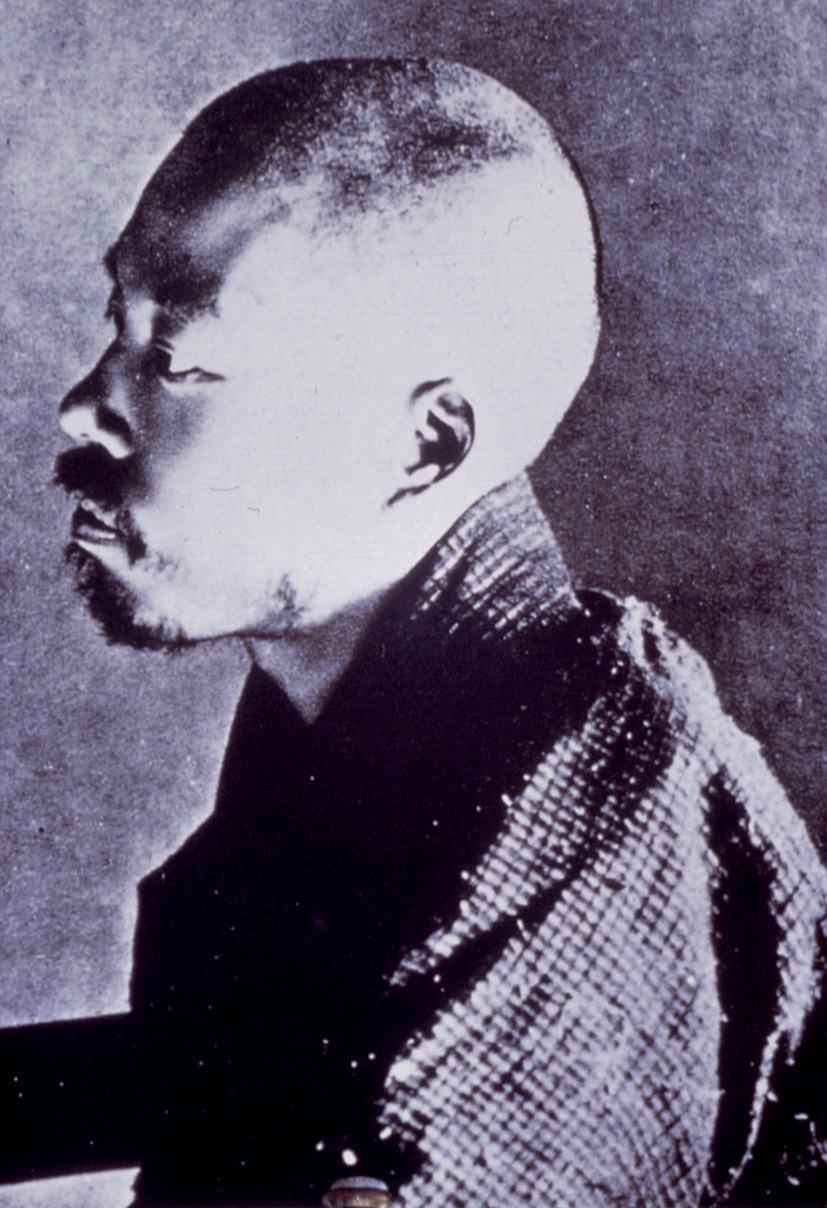
\includegraphics[height=0.9\textheight]{masaoka}\\[1em]
        \large{\FS 作~者~像}
    \end{figure}
\end{center}

\newpage
{\FS
    正冈子规(1867—1902),爱媛县松山市人,本名常规,别号獭祭书屋主人、竹子乡下人等。父隼太是松山藩士,母八重是著名汉学家大原观山之女。子规六岁丧父,由母亲抚养成人,年幼时跟外祖父大原观山和土屋文明学汉籍,奠定了深厚的汉学基础。十二岁写绝句『闻子规』:「一声孤月下,啼血不可闻,关夜空欹枕,故乡万里云。」显示出他的才华。一八八九年五月九日,二十三岁的子规开始咯血,是年取别号子规。他晚年长期卧病,但并不悲伤绝望,能乐观自处,在病床上写了动人的随笔『墨汁一滴』、『仰卧漫录』、『病床六尺』等。病情日渐恶化,逝世时才三十六岁。

    子规的一生虽然短暂,但他以坚韧不拔的努力,在明治时代文学史上留下了不可磨灭的功绩。他主张俳句和短歌应该革新,向江户末期的陈规陋习挑战,写了『獭祭屋俳话』、『俳句分类』、『俳谐大要』、『俳人芜村』等力作,在俳句创作上特别推崇芜村,使人们对芜村作品的艺术价值有了新的认识。

    子规作为俳人,可以说是一位承前启后的人物。他与芭蕉、芜村、一茶相比,因所处的时代、境遇和个人气质不同,俳风也就各异。子规主张「感情的文学,即纯粹的文学」,「美的标准,在于美的感情」。他的俳句,看来并非呕心沥血的苦吟,写景抒情,多为即兴之作。虽然他说过:「比起人事来,我更爱花鸟风月。」但晚年他也写了自以为较难写的人事写生句。可能是因为他在理论上过于强调写生,致使想象力不够丰富,生活又为病床所限,所以笔下的境界不够宽阔。他效法芜村的色彩美,也有汉诗的情调,俳风平易单纯,简洁明快,独树一帜。

    在短歌方面,他于一九〇二年发表『致歌人书』,又组织「根岸短歌会」,提倡短歌的革新,要求以写生法创作短歌,自己也效法『万叶集』的精神作了不少短歌,在歌坛有一定影响。

    附带说一下:我译的芭蕉、芜村、一茶的若干俳句发表以后,对我国友好的日本作家水上勉先生有一次对我说:「是否也译些正冈子规的俳句?」他这么一提,鼓起了我的勇气,我就开始阅读有关正冈子规的资料,并根据『子规全集』(共22卷,讲谈社1975年版)试译了俳句七十八首。译文也许未能传达原作的神韵,请读者指正。
}

\newpage

\section{\FK 新年}

\setcounter{haikucounter}{0}

\begin{haiku}
    {\FH \ruby{初鶏}{はつとり}の、\ruby{枕}{まくら}の上に、うたひける。}

    {\FK 正欲睡眠鸡报晓,岁序转新春。}
\end{haiku}

\begin{haiku}
    {\FH \ruby{梅}{うめ}いけて、\ruby{礼者}{れいしゃ}ことわる、\ruby{病}{やまい}かな。}

    {\FK 瓶插梅花共贺春,谢客只因是病身。}
\end{haiku}

\begin{haiku}
    {\FH \ruby{民}{たみ}の春、\ruby{同胞}{どうほう}三千、九百万。}

    {\FK 同胞三千九百万,共庆过新年。}
\end{haiku}

\section{\FK 春}

\setcounter{haikucounter}{0}

\begin{haiku}
    {\FH 春の山、\ruby{焼}{や}いたあとから、\ruby{笑}{わら}ひけり。}

    {\FK 春山烧后露笑容。}
\end{haiku}

\begin{haiku}
    {\FH あたゝかな、雨がふるなり、\ruby{枯葎}{かれむぐら}。}

    {\FK 温雨纷纷下,蔓草枯干不见芽。}

    {\FT 注:温雨即初春的雨,有暖意。}
\end{haiku}

\begin{haiku}
    {\FH 春雨や、\ruby{唐撫子}{からなでしこ}の、死を\ruby{惜}{おし}む。}

    {\FK 春雨霏霏,哀哉石竹凋萎!\footnote{\FT 此句实为高滨虚子所作。}}
\end{haiku}

\begin{haiku}
    {\FH \ruby{陽炎}{かげろう}や、日本の土に、\ruby{殯}{かりもがり}。}

    {\FK 游丝呀,埋葬东瀛泥土下!}

    {\FT 注:以上两句是哀悼子规的中国弟子苏山人之作。苏山人(1881—1902)姓罗名朝斌,字卧云,号听松,江苏苏州人,父罗庚龄为清朝驻日公使何如璋的译员,母是日本人。苏山人自幼喜爱文学诗歌,后拜正冈子规为师,交游颇广。他的俳句被收在子规编辑的『春夏秋冬』、『明治俳句』专集中。一九〇二年春因病在东京逝世,年仅二十二岁。}
\end{haiku}

\begin{haiku}
    {\FH 島々に、\ruby{灯}{ひ}をともしけり、春の海}

    {\FK 岛岛点起了灯火,春之海啊。}
\end{haiku}

\begin{haiku}
    {\FH \ruby{一桶}{いちおけ}の、\ruby{藍}{あい}\ruby{流}{なが}しけり、春の川。}

    {\FK 春日河川上,正是一桶靛蓝流。}

    {\FT 注:这是子规流畅体。作者把春天河川的水比作一桶流动的蓝颜料,这景象在乡下有染坊的地方可以看到。\footnote{\FT 此句出自『病床六尺』,据子规自注,确实是一桶随波飘荡的蓝色颜料,而不是形容河水被染成蓝色。}}
\end{haiku}

\begin{haiku}
    {\FH 春風に、\ruby{零}{こぼれ}て赤し、\ruby{歯}{はみ}\ruby{磨}{がき}\ruby{粉}{こ}。}

    {\FK 洒落春风牙粉红。}

    {\FT 注:子规早晨刷牙时因咯血而染红了牙粉。此句用红白的色彩感来描写病状,没有悲伤意。}
\end{haiku}

\begin{haiku}
    {\FH 春の日や、\ruby{病床}{びょうしょう}にして、絵の\ruby{稽古}{けいこ}。}

    {\FK 春日病床上,学画来消遣。}

    {\FT 注:子规喜画,但无老师,只把花果放在床边,随笔写生。}
\end{haiku}

\begin{haiku}
    {\FH とろとろと、\ruby{左官}{さかん}眠るや、\ruby{燕}{つばくらめ}。}

    {\FK 泥工打瞌睡,燕子正交飞。}

    {\FT 注:此句写农村的泥工盖新房午休时的情景。}
\end{haiku}

\begin{haiku}
    {\FH ひらひらと、風に流れて、\ruby{蝶}{ちょう}一つ。}

    {\FK 蝴蝶翩翩飞去,风吹又飞回。}
\end{haiku}

\begin{haiku}
    {\FH \ruby{茨}{いばら}にかけし、\ruby{胡蝶}{こちょう}の羽の、\ruby{破}{やぶ}れたる。}

    {\FK 蝴蝶碰荆棘,刺破了翅膀。}

    {\FT 注:美丽的翅膀受了损伤,令人惋惜。}
\end{haiku}

\begin{haiku}
    {\FH \ruby{白魚}{しらうお}や、\ruby{椀}{わん}の中にも、角田川。}

    {\FK 银鱼碗里鲜,联想角田川。}

    {\FT 注:银鱼在日语中叫白鱼,角田川现称隅田川。}
\end{haiku}

\begin{haiku}
    {\FH \ruby{若鮎}{わかあゆ}の、二手になりて、\ruby{上}{のぼ}りけり。}

    {\FK 石手川出合渡}

    {\FK 小香鱼,分两路溯流游去。}

    {\FT 注:石手川出合渡是松山市内的重信川与郊外的石手川合流的渡口,活泼的小香鱼在合流处分二路溯流而上。}
\end{haiku}

\begin{haiku}
    {\FH 茶屋もなく、\ruby{酒屋}{さかや}も見えず、花一木。}

    {\FK 茶楼酒馆无踪迹,唯见娇艳花一枝。}
\end{haiku}

\begin{haiku}
    {\FH 桃梅を、笑へば梅も、桃を笑らふ。}

    {\FK 国会}

    {\FK 桃嘲梅来梅笑桃。}
\end{haiku}

\begin{haiku}
    {\FH 人載せて、牛載せて桃の、渡し哉。}

    {\FK 载人又载牛,喧闹桃渡口。}
\end{haiku}

\begin{haiku}
    {\FH 紅梅の、散りぬ\ruby{淋}{さび}しき、枕元。}

    {\FK 红梅花散落,寂寞枕头边。}
\end{haiku}

\begin{haiku}
    {\FH 夢に美人、来れり\ruby{曰}{いわ}く、梅の精と。}

    {\FK 梦里美人来,说是梅花精。}

    {\FT 注:这是妖艳句,颇有芜村的风格。}
\end{haiku}

\begin{haiku}
    {\FH 僧や俗や、梅活けて\ruby{発句}{はっく}、十五人。}

    {\FK 松山松风会席上}

    {\FK 花瓶插红梅,僧俗俳句十五人。}
\end{haiku}

\begin{haiku}
    {\FH \ruby{鞦韆}{しゅうせん}の、影静かなり、梨花の月。}

    {\FK 秋千影静静,梨花月有阴。}

    {\FT 注:此句意境与苏轼『春宵』中的「花有清香月有阴……秋千院落夜沉沉」略同。}
\end{haiku}

\begin{haiku}
    {\FH 一つ落ちて、二つ落ちたる、\ruby{椿}{つばき}哉。}

    {\FK 山茶花啊,落了一朵,落了两朵。}

    {\FT 注:这三句略似小幅写生画,给人留下鲜明印象,句中有时间的推移,使人仿佛目睹艳丽的景物。}
\end{haiku}

\begin{haiku}
    {\FH 山吹の、雨やガラスの、窓の外。}

    {\FK 玻璃窗外,棠棣花雨飘。}
\end{haiku}

\section{\FK 夏}

\setcounter{haikucounter}{0}

\begin{haiku}
    {\FH 夏嵐、\ruby{机上}{きじょう}の\ruby{白紙}{はくし}、飛び\ruby{尽}{つく}す。}

    {\FK 夏日山风来,桌上白纸尽飞去。}
\end{haiku}

\begin{haiku}
    {\FH 五月雨や、\ruby{けふ}{きょう}も上野を、見てくらす。}

    {\FK 梅雨时节,看厌上野山色。}
\end{haiku}

\begin{haiku}
    {\FH \ruby{陣笠}{じんがさ}を、着た人もある、\ruby{田植}{たうえ}哉。}

    {\FK 插秧农田里,还有戴盔人。}

    {\FT 注:藩士退役归田,从事农耕,插秧时还戴着战盔。此句表示时代已变化,仍留旧迹象。}
\end{haiku}

\begin{haiku}
    {\FH 暁や、白帆過ぎ行く、\ruby{蚊帳}{かや}の外。}

    {\FK 拂晓时分,白帆驶过蚊帐外。}

    {\FT 注:子规在海边须磨疗养院的卧室里,晨曦照在绿色的蚊帐上,此时他意外地看见白帆在海上驶过。}
\end{haiku}

\begin{haiku}
    {\FH \ruby{柳}{やなぎ}伐って、\ruby{翡翠}{かわせみ}\ruby{遂}{つい}に、来ずなりぬ。}

    {\FK 柳树被伐采,终于不见翡翠来。}

    {\FT 注:子规认为梅与莺、竹与雀、杨柳与翡翠的配合,虽是陈旧的程式,但也有其美感。翡翠总是站在水边的柳枝上想啄食水中的游鱼,柳树既被砍掉,翡翠失去立脚点,就到别处去了。}
\end{haiku}

\begin{haiku}
    {\FH \ruby{看}{かん}\ruby{護}{ご}\ruby{婦}{ふ}や、うたゝ寝さめて、\ruby{蝿}{はえ}を打つ。}

    {\FK 看护妇打瞌睡,醒来拍苍蝇。}

    {\FT 注:伺候子规的看护妇瞌睡醒后,不好意思,拿蝇拍打苍蝇,这写出了一种心理状态。}
\end{haiku}

\begin{haiku}
    {\FH 林檎くふて、牡丹の前に、死なん哉。}

    {\FK 饱啖苹果后,死在牡丹前。}

    {\FT 注:一八九六年五月十七日,子规从中国归国的途中,在船上咯血,二十八日进入神户病院。翌年四月五日做了两次手术。一八九九年五月,子规发烧、失眠、腰痛,食欲不振,病势较重,因不堪其苦,故吟此辞世句。}
\end{haiku}

\begin{haiku}
    {\FH \ruby{銀屏}{ぎんびょう}や、\ruby{崩}{くず}れんとする、白牡丹。}

    {\FK 华丽银屏前,烂漫将谢白牡丹。}

    {\FT 注:银屏配白牡丹,那是满屋生辉的景色,但此句只写白牡丹盛开将谢的状态。这是艳丽句体。}
\end{haiku}

\begin{haiku}
    {\FH 土\ruby{一塊}{いっかい}、牡丹いけたる、其下に。}

    {\FK 自题}

    {\FK 牡丹花瓶下,泥土一块。}

    {\FT 注:一九〇二年五月,子规为病情所苦而作此句,题在香取秀真为他塑制的石膏像背面。作者认为自己死之将至,犹如艳丽的牡丹花下的一块泥土。}
\end{haiku}

\begin{haiku}
    {\FH 赤き薔薇、白き薔薇皆、さみだるゝ。}

    {\FK 红蔷薇,白蔷薇,湿润梅雨水。}
\end{haiku}

\begin{haiku}
    {\FH 薔薇を剪る、\ruby{鋏刀}{はさみ}の音や、\ruby{五月}{さつき}\ruby{晴}{ばれ}。}

    {\FK 听得蔷薇剪刀声,正是五月梅雨晴。}
\end{haiku}

\begin{haiku}
    {\FH 朝顔や、紫しぼる、朝の雨。}

    {\FK 牵牛花色艳,染得晨雨亦紫妍。}

    {\FT 注:晨雨接触牵牛花,染上紫艳颜色,染字成为句的主眼,上下全活了。}
\end{haiku}

\begin{haiku}
    {\FH \ruby{蕣}{あさがお}や、君いかめしき、文学士。}

    {\FK 牵牛正值开花时,迎接堂堂文学士。}

    {\FT 注:夏目漱石对文部省授给文学博士的称名,十分讨厌,曾坚决谢绝,但谢绝不了。子规在此句中,用「堂堂」二字,有点打趣。}
\end{haiku}

\begin{haiku}
    {\FH 青梅や、黄梅やうつる、\ruby{軒}{のき}らんぷ。}

    {\FK 檐下油灯明,青梅黄梅相照映。}

    {\FT 注:梅雨季节,梅子未熟的叫青梅,熟的叫黄梅。}
\end{haiku}

\begin{haiku}
    {\FH 若竹や、四五本青き、庭の\ruby{隅}{すみ}。}

    {\FK 一角庭院边,嫩竹青青四五竿。}
\end{haiku}

\begin{haiku}
    {\FH 舟行くや、\ruby{小鬢}{こびん}にさはる、\ruby{蓮}{はす}の花。}

    {\FK 舟行在莲塘,莲花碰触小鬓上。}

    {\FT 注:梁武帝有五言诗:「采莲南塘秋,莲花过人头。」子规把「过」改为「碰」,都是美丽的画面。}
\end{haiku}

\section{\FK 秋}

\setcounter{haikucounter}{0}

\begin{haiku}
    {\FH 天の川、こぼれ落ちたる、星一つ。}

    {\FK 夜凉如水,银河岸畔,星一颗。}
\end{haiku}

\begin{haiku}
    {\FH \ruby{門}{かど}を出て、十歩に秋の、海廣し。}

    {\FK 出门走十步,秋日海天阔。}
\end{haiku}

\begin{haiku}
    {\FH 旅の旅、又その旅の、秋の風。}

    {\FK 旅行又旅行,秋风尽在旅途中。}

    {\FT 注:这是一八九二年所作的俳句,写他在十月间无休止的旅行,又在旅途中感到秋风的寒意,同时也反映他是在人生的道路上。}
\end{haiku}

\begin{haiku}
    {\FH 秋の山、\ruby{御幸寺}{みゆきじ}と申し、天狗住む。}

    {\FK 秋山御幸寺,天狗住其中。}

    {\FT 注:山在松山北郊,人们叫它作御幸寺。山形怪异,相传有天狗在那里,令人恐惧。天狗是想象中的怪物,住在深山中,状如人,红脸高鼻,有翅膀,飞行自如。}
\end{haiku}

\begin{haiku}
    {\FH 長き夜や、孔明死する、三國志。}

    {\FK 长夜览读『三国志』,正到孔明病殁时。}
\end{haiku}

\begin{haiku}
    {\FH 長き夜の、面白きかな、\ruby{水滸傳}{すいこでん}。}

    {\FK 阅读『水浒传』,夜长妙趣多。}

    {\FT 注:子规自少年时代,便爱读军事历史小说之类,『水浒传』、『三国演义』也是他爱读的书。}
\end{haiku}

\begin{haiku}
    {\FH 長き夜や、人灯を取って、庭に行く。}

    {\FK 人提灯火穿院去,夜里依然又静寂。}

    {\FT 注:写静中有动,动后仍归于静,这是着重于听觉的句子。}
\end{haiku}

\begin{haiku}
    {\FH 行く我に、とどまる\ruby{汝}{なれ}に、秋二つ。}

    {\FK 别漱石}

    {\FK 我去你留,两个秋。}

    {\FT 注:子规从松山要去东京,夏目漱石仍旧逗留松山。两人分别,时在秋天,惜别又叹境遇不同,巧妙地用了两个秋。}
\end{haiku}

\begin{haiku}
    {\FH \ruby{芋}{いも}の\ruby{用意}{ようい}、酒の用意や、人遲し。}

    {\FK 煮芋又备酒,宾客何来迟。}

    {\FT 注:一八九七年八月十七日,在上野元光院赏月,又听筑前琵琶。到会者约二十人。此句写月出前的准备工作。}
\end{haiku}

\begin{haiku}
    {\FH あるが中に、\ruby{詩人}{しじん}\ruby{痩}{や}せたり、月の宴。}

    {\FK 赏月雅会里,诗人貌清瘦。}

    {\FT 注:雅会中的诗人,指汉诗人本田种竹山人之辈,子规和他交往,谈论汉诗,曾有汉诗『访种竹君听诗话而还』。}
\end{haiku}

\begin{haiku}
    {\FH ある僧の、月も待たずに、歸りけり。}

    {\FK 旧历八月十七日元光院}

    {\FK 不待明月出,有僧竟自归。}

    {\FT 注:一八九八年相约于中秋后两天赏「立待月」,子规也稍微迟到参加了。但其中释清潭不知何故却早离席。高滨虚子以为此句有弦外之音,说此僧人胸无点墨,不能强为吟咏,故早退席。}
\end{haiku}

\begin{haiku}
    {\FH \ruby{病床}{びょうしょう}の、\ruby{呻}{うめ}きに\ruby{和}{なご}して、秋の蝉。}

    {\FK 病床苦呻吟,秋蝉来唱和。}

    {\FT 注:到了秋天,蝉断断续续衰弱的叫声,跟病者的呻吟声,有点合调。}
\end{haiku}

\begin{haiku}
    {\FH \ruby{木犀}{もくせい}や、母が\ruby{教}{をし}ふる、\ruby{二絃琴}{にげんきん}。}

    {\FK 木樨花正发,母教二弦琴。}
\end{haiku}

\begin{haiku}
    {\FH 月\ruby{落}{おち}て、\ruby{江村}{こうそん}\ruby{蘆}{あし}の、花白し。}

    {\FK 江村月夜芦花白。}
\end{haiku}

\begin{haiku}
    {\FH \ruby{骨}{こ}も見えず、むくろも見えず、草の花。}

    {\FK 吊古战场}

    {\FK 尸骨皆不见,唯有草花妍。}
\end{haiku}

\begin{haiku}
    {\FH \ruby{柿}{かき}食へば、\ruby{鐘}{かね}が鳴るなり、\ruby{法隆寺}{ほうりゅうじ}。}

    {\FK 在法隆寺茶店小憩}

    {\FK 我尝柿子时,钟鸣法隆寺。}

    {\FT 注:吃柿子时听到钟声,两者虽无关联,只因为是同时发生的事,就把它们联系起来。}
\end{haiku}

\begin{haiku}
    {\FH 三千の、俳句を\ruby{閲}{けみ}し、柿二つ。}

    {\FK 俳句检阅三千首,枕边柿子两个。}

    {\FT 注:子规在『日本』报刊上创设俳句栏,是他的革新事业的中心。有一天要夜以继日地看来稿俳句三千首,从中选用,工作颇为繁忙。枕边放着爱吃的两个柿子。「两个」和「三千」是数字的照应。}
\end{haiku}

\begin{haiku}
    {\FH 冬近き、嵐に折れし、\ruby{鷄頭}{けいとう}哉。}

    {\FK 幼嫩鸡冠花,那堪飙风刮?}

    {\FT 注:子规酷爱鸡冠花,以拟人法描写它。}
\end{haiku}

\begin{haiku}
    {\FH 鷄頭の、十本ばかり、百姓家。}

    {\FK 寻常百姓家,将开十蕊鸡冠花。}
\end{haiku}

\begin{haiku}
    {\FH \ruby{案山子}{かかし}物、言て\ruby{猶}{なお}淋しぞ、秋の\ruby{暮}{くれ}。}

    {\FK 稻草人也感寂寞,当此秋之暮。}
\end{haiku}

\begin{haiku}
    {\FH 柳散り、菜\ruby{屑}{くず}流るゝ、小川哉。}

    {\FK 根岸音无川}

    {\FK 柳叶已凋萎,菜屑小川漂。}

    {\FT 注:根岸与日暮里之间有条小川,名叫音无川。秋冬时附近居民在这小川洗净蔬菜。}
\end{haiku}

\begin{haiku}
    {\FH \ruby{白萩}{しろはぎ}の、しきりに露を、こぼしけり。}

    {\FK 风吹白色胡枝子,花露点点滴。}

    {\FT 注:这是写秋天庭院的美,秋风吹拂白萩花露滴落的情景。}
\end{haiku}

\begin{haiku}
    {\FH 驚くや、夕顔落ちし、\ruby{夜半}{よわ}の音。}

    {\FK 夜半惊醒梦,瓠瓜落地声。}

    {\FT 注:某夜深时,有一种声音,使子规从梦中惊醒过来,后来才知道是院子的瓠瓜棚上结的瓠瓜落地的声音。声音微小,子规也这么震动,可见他的身体衰弱。}
\end{haiku}

\begin{haiku}
    {\FH 草花を、畫く日課や、秋に入る。}

    {\FK 入秋时节,绘草描花作日课。}

    {\FT 注:子规好作画,入秋画画,聊以自慰,将盆裁的草花摆到枕边作写生之用。据云最初画的草花是秋海棠。此句是他的生活写照。}
\end{haiku}

\begin{haiku}
    {\FH \ruby{糸瓜}{へちま}\ruby{咲}{さい}て、\ruby{痰}{たん}のつまりし、仏かな。}

    {\FK 丝瓜放蕊时,痰塞成佛去。}
\end{haiku}

\begin{haiku}
    {\FH 痰一斗、糸瓜の水も、間にあはず。}

    {\FK 良药丝瓜水,难治一斗痰。}
\end{haiku}

\begin{haiku}
    {\FH をととひの、糸瓜の水も、取らざりき。}

    {\FK 前日丝瓜水,不曾饮入嘴。}

    {\FT 注:丝瓜是止咳消痰的药材,曾在自己的院子做棚种植\footnote{{\FT 前文有述子规的院子里有瓠瓜棚,瓠瓜和丝瓜不是同一种植物。丝瓜的学名} \emph{Lagenaria siceraria} var. \emph{hispida} {\FT ,和瓠瓜同属葫芦科。}},入药用。}

    {\FT 以上是绝笔的三首俳句。子规的病况,一九〇二年九月十日起,两腿浮肿,一点也不能动弹,但精神却很平稳,意识到死神已经迫近,终于在十九日午前一时逝世。}
\end{haiku}

\section{\FK 冬}

\setcounter{haikucounter}{0}

\begin{haiku}
    {\FH \ruby{小夜}{さよ}\ruby{時雨}{しぐれ}、上野を虚子の、來つゝあらん。}

    {\FK 病中}

    {\FK 夜半时雨降,虚子可从上野来?}

    {\FT 注:子规殷切希望弟子高滨虚子早一点来。}
\end{haiku}

\begin{haiku}
    {\FH いくたびも、雪の深さを、\ruby{尋}{たず}ねけり。}

    {\FK 病中雪}

    {\FK 频频寻问,积雪深几许?}

    {\FT 注:久卧病床的子规,总想接触外界,问了妹妹,又问妈妈,使她们不得不跑出门外看雪,再回答子规。这句写出子规难以抑制挂念积雪的心情,是他的代表作之一。}
\end{haiku}

\begin{haiku}
    {\FH 冬\ruby{籠}{こもり}、日記に梦を、書きつける。}

    {\FK 目记存梦境,闭门严冬静。}
\end{haiku}

\begin{haiku}
    {\FH 雪の跡、木履\ruby{草鞋}{わらじ}の、別れかな。}

    {\FK 雪中送客去,留下草鞋木屐痕。}
\end{haiku}

\begin{haiku}
    {\FH 冬\ruby{枯}{がれ}や、巡査に\ruby{吠}{ほ}える、里の犬。}

    {\FK 荒寒少客行,村犬吠巡警。}
\end{haiku}

\begin{haiku}
    {\FH \ruby{鷹狩}{たかがり}や、豫陽の太守、武を\ruby{好}{この}む。}

    {\FK 尚武豫阳太守,放鹰猎获野兽。}
\end{haiku}

\begin{haiku}
    {\FH しぐるゝや、むれて押しあふ、桶の\ruby{鮒}{ふな}。}

    {\FK 鲫鱼惊阵雨,竞相逃避一桶里。}

    {\FT 注:屋外桶里的鲫鱼,因阵雨滴落,在狭窄的桶里竞相逃避,这是写小景、近景的俳句。}
\end{haiku}

\begin{haiku}
    {\FH \ruby{暖爐}{だんろ}\ruby{焚}{た}くや、\ruby{玻璃}{はり}窓外の、風の松。}

    {\FK 室中炉火盛,玻璃窗外松涛声。}
\end{haiku}

\begin{haiku}
    {\FH 水仙も、處を得たり、庭の隅。}

    {\FK 贺新居}

    {\FK 水仙得其所,庭隅自不俗。}
\end{haiku}

\begin{haiku}
    {\FH 梅活けて、君待つ\ruby{庵}{いお}や、\ruby{大}{おお}\ruby{三十}{みそ}\ruby{日}{か}。}

    {\FK 漱石约来寓}

    {\FK 时逢除夕岁将尽,插就梅花等待君。}
\end{haiku}

\chapter[{\FM 夏目漱石}]{\FM \ruby{夏}{なつ}\ruby{目}{め}\ruby{漱}{そう}\ruby{石}{せき}}

\begin{center}
    \begin{figure}
        \centering
        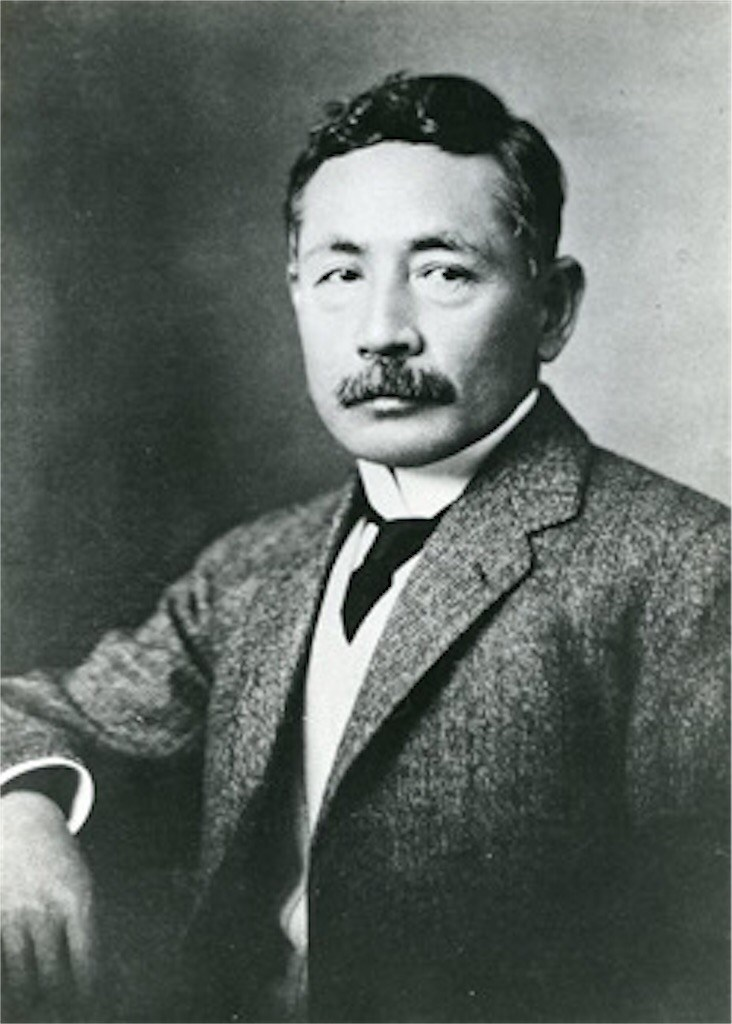
\includegraphics[height=0.9\textheight]{natsume}\\[1em]
        \large{\FS 作~者~像}
    \end{figure}
\end{center}

\newpage

{\FS
    夏目漱石(1867—1916)生于江户牛込马场下横町的一个小官吏的家庭,本名金之助。一八九三年东京帝国大学英文科毕业后,先后在东京专门学校、东京高等师范学校、爱媛县松山中学教英文。一九〇〇年被文部省派往英国伦敦留学,研究英国文学。留学期间,备受冷落,极不愉快。回国后对当时社会非常愤懑。一九〇五年在『杜鸥』杂志上发表『我是猫』(长篇讽刺小说),一九〇六年发表小说『哥儿』,批判教育界不良现象,于是声名大振,同年发表俳句情趣的小说『旅宿』,主人公是一个画家,避开讨厌的世俗,外出旅行,寻求澄清心境的桃源。一九〇七年他辞去教职,任『朝日新闻』文艺栏主编,在该报发表三部曲『三四郎』、『其后』和『门』,反映了知识分子在黑暗社会寻求出路的窘状。他遂成为日本杰出的批判现实主义作家。

    夏目漱石在思想上受了儒学与禅宗的影响。在创作风格上属于「余裕派」,主张以旁观者的立场和悠然自得的态度,吟咏自然、艺术和人生。他特别赏识「读万卷书而为万里游」的名言,一位日本评论家说:「其文雄俊博大,卓然有奇气。」

    夏目漱石少年时代从东京第一中学转入二松学舍学习汉学,并练习写作,也曾想以汉学立身。晚年写很多汉诗,对于格律、平仄、押韵和对仗运用自如。诗虽多无题,而情味甚浓,兹请读其临终前二旬间写的一首七律:
    \begin{center}
        真踪寂寞杳难寻,欲抱虚怀步古今。

        碧水碧山何有我,盖天盖地是无心。

        依稀暮色月离草,错落秋声风在林。

        眼耳双忘身亦失,空中独唱白云吟。
    \end{center}

    他很早就写俳句,一八九五年在松山中学任教时,与正冈子规同住过愚陀佛庵公寓,过从甚密,参加过子规指导的松风会活动。一生所写的俳句约达二四五〇首。在松山写的俳句占三分之一,并用过愚陀佛的笔名。他和子规是同龄人,曾受子规的影响,尊重子规所倡导的写实,但也发展自己浪漫气氛与洒脱畅达的特色。子规曾赞其俳句「雄键,无往而不雄健;真诚,无往而不真诚」。夏目漱石写作俳句的热情后来减退,专事小说创作。一九一五年开始在『朝日新闻』上连载长篇小说『明暗』,但还没写完就因病逝世,终年五十岁。本集中所选四十六首俳句,都是根据『夏目漱石全集』第二十三卷(岩波书店1984年版)翻译的。
}

\newpage

\section{\FK 新年}

\setcounter{haikucounter}{0}

\begin{haiku}
    {\FH \ruby{五斗米}{ごとべい}を、\ruby{餅}{もち}にして喰ふ、春来たり。}

    {\FK 新春已来到,五斗米做饼吃。}
\end{haiku}

\begin{haiku}
    {\FH \ruby{金泥}{きんでい}の、鶴や\ruby{朱塗}{しゅぬり}の、\ruby{屠蘇}{とそ}の\ruby{盆}{ぼに}。}

    {\FK 泥金仙鹤画,涂朱屠苏杯。}
\end{haiku}

\begin{haiku}
    {\FH 温泉や、水\ruby{滑}{なめ}らかに、去年の\ruby{垢}{あか}。}

    {\FK 温泉水滑,洗去旧年油垢。}

    {\FT 注:「温泉水滑」取自白居易『长恨歌』中的「温泉水滑洗凝脂」。}
\end{haiku}

\begin{haiku}
    {\FH \ruby{光琳}{こうりん}の、\ruby{屏風}{びょうぶ}に咲くや、\ruby{福寿草}{ふくじゅそう}。}

    {\FK 福寿草花,开在光琳屏风上。}

    {\FT 注:福寿草即侧金盏花,黄色多瓣,增添新春气氛。光琳即尾形光琳(1658—1716),日本名画家。}
\end{haiku}

\section{\FK 春}

\setcounter{haikucounter}{0}

\begin{haiku}
    {\FH \ruby{馬子唄}{まごうた}や、\ruby{白髪}{しらが}も染めで、暮るゝ春。}

    {\FK 马夫歌声处,白发对暮春。}

    {\FT 注:小说『旅宿』载此句,指山村老太婆难耐凄凉,几经岁月数着过路的马。}
\end{haiku}

\begin{haiku}
    {\FH 春風や、\ruby{惟然}{いぜん}が耳に、馬の鈴。}

    {\FK 惟然耳边声,春风吹马铃。}

    {\FT 注:广漱惟然是江户时代前期俳人芭蕉的门人。句写登山之后,景象寂寥。似以惟然自况。}
\end{haiku}

\begin{haiku}
    {\FH 春寒し、\ruby{墓}{はか}に\ruby{懸}{か}けたる、季子の剣。}

    {\FK 春寒暮树,挂着季子的剑。}

    {\FT 注:春秋吴国季札给逝世的徐君赠剑的故事。}
\end{haiku}

\begin{haiku}
    {\FH 人に死し、鶴に生れて、\ruby{冴返}{さえかえ}る。}

    {\FK 人死转生鹤,高洁又清和。}

    {\FT 注:有的评论家认为此作富于浪漫主义幻想,有着离俗的格调,是个几乎难以企及的秀句。}
\end{haiku}

\begin{haiku}
    {\FH \ruby{腸}{はらわた}に、春\ruby{滴}{したた}るや、\ruby{粥}{かゆ}の味。}

    {\FK 粥味滴滴香,春入肠胃。}

    {\FT 注:作者患胃溃疡,在伊豆修养寺疗养,病情好转,才得进粥食,有苏生的喜悦。}
\end{haiku}

\begin{haiku}
    {\FH 落ちさまに、\ruby{虻}{あぶ}を\ruby{伏}{ふ}せたる、椿哉。}

    {\FK 虻虫藏在茶花里,正将落地时。}

    {\FT 注:此句抓住瞬间的感触,轻小的虻虫,伏在沉甸甸的山茶花蕊上行将落地。}
\end{haiku}

\begin{haiku}
    {\FH 梅の奥に、誰やら住んで、\ruby{幽}{かす}かな灯。}

    {\FK 谁住在梅花丛里,幽幽灯火明。}

    {\FT 注:此句写梦幻的诗境,如见『源氏物语』的画卷,充满着古典美。}
\end{haiku}

\begin{haiku}
    {\FH 梅に対す、\ruby{和靖}{わせい}の\ruby{髭}{ひげ}の、白きかな。}

    {\FK 和靖面对梅花,胡须已经雪白。}
\end{haiku}

\begin{haiku}
    {\FH 木蓮の、花\ruby{許}{ばか}りなる、空を\ruby{瞻}{み}る。}

    {\FK 伫立抬头看,木兰花满天。}

    {\FT 注:这是载于小说『旅宿』的写景句。}
\end{haiku}

\begin{haiku}
    {\FH \ruby{菫}{すみれ}ほどな、小さき人に、生まれたし。}

    {\FK 愿如紫地丁,生为渺小人。}

    {\FT 注:此句是作者内心的表白,含有禅境的人生观。厌弃丑恶的现世,寄情于自然界的小花草。}
\end{haiku}

\begin{haiku}
    {\FH \ruby{萱草}{かんぞう}の、一輪咲きぬ、草の中。}

    {\FK 草丛中,萱花开一朵。}

    {\FT 注:中日都称萱草为忘忧草。}
\end{haiku}

\begin{haiku}
    {\FH 海棠の、精が出てくる、月夜かな。}

    {\FK 朦胧月夜色,浮现海棠精。}

    {\FT 注:此句有芜村的幻想情调,写春宵里海棠变成了妖精。于此联想到陆游『春愁曲』:「蜀姬双鬓娅姹娇,醉看恐是海棠妖。」}
\end{haiku}

\section{\FK 夏}

\setcounter{haikucounter}{0}

\begin{haiku}
    {\FH 雲の\ruby{峰}{みね}、\ruby{雷}{らい}を封じて、\ruby{聳}{そび}えけり。}

    {\FK 云峰耸太空,封闭大雷声。}
\end{haiku}

\begin{haiku}
    {\FH 無人島の、天子とならば、涼しかろ
    。}

    {\FK 无人岛上为天子,定觉清凉吧。}

    {\FT 注:从英国回国后,有苦闷厌世感,想出一个超现实的无人国。句意虽然逃避了现实的重压,还是不能称心。这句意匠崭新,着想奇拔。}
\end{haiku}

\begin{haiku}
    {\FH 灯を\ruby{消}{け}せば、涼しき星や、窓に入る。}

    {\FK 灯火熄灭后,冷星入窗来。}
\end{haiku}

\begin{haiku}
    {\FH 大手より、源氏寄せたり、青嵐。}

    {\FK 青岚中,源氏从正门迫攻。}

    {\FT 注:青岚,夏天吹过万绿丛中的风。写日本源平争霸时,源氏的军事优势,是印象鲜明的咏史句。}
\end{haiku}

\begin{haiku}
    {\FH こうろげの、飛ぶや\ruby{木魚}{もくぎょ}の、声の下。}

    {\FK 黄昏敲响木鱼,吐出白昼蚊虫。}

    {\FT 注:此句写静寂幽暗的佛堂,僧人敲木鱼念经,蚊子从木鱼里飞出也发微弱的叫声,有点轻妙的呼应趣味。}
\end{haiku}

\begin{haiku}
    {\FH ほのぼのと、舟押し出すや、\ruby{蓮}{はす}の中。}

    {\FK 莲花塘里面,隐约推舟出。}

    {\FT 注:此句象一幅绘画,写着隐约的美。}
\end{haiku}

\section{\FK 秋}

\setcounter{haikucounter}{0}

\begin{haiku}
    {\FH 日の入や、\ruby{五重}{いつえ}の塔に、残る秋。}

    {\FK 夕照五重塔,感叹秋已残。}
\end{haiku}

\begin{haiku}
    {\FH \ruby{手}{た}向くべき、\ruby{線}{せん}\ruby{香}{こう}もなくて、暮の秋
。}

{\FK 在伦敦得子规讣闻。}

{\FK 无香可祭奠,那暮秋时节。}
\end{haiku}

\begin{haiku}
    {\FH \ruby{霧黄}{きりき}なる、市に動くや、影法師。}

    {\FK 雾都黄昏时,恍动他身影。}

    {\FT 注:以上二句作于一九〇二年秋。伦敦是名闻世界的雾都。在雾都中仿佛看到子规摇曳的身影。抒写他听到子规去世时沉闷的心情。}
\end{haiku}

\begin{haiku}
    {\FH 枕\ruby{辺}{べ}や、星別れんと、する\ruby{晨}{あした}。}

    {\FK 清晨枕席畔,双星惜别时。}

    {\FT 注:此句写作者与爱妻中根镜子的惜别深情。}
\end{haiku}

\begin{haiku}
    {\FH 別るゝや、夢一\ruby{筋}{すじ}の、天の川。}

    {\FK 离别情难遣,梦隔一天河。}
\end{haiku}

\begin{haiku}
    {\FH 秋の江に、打ち込む\ruby{杭}{くい}の、\ruby{響}{ひびく}かな。}

    {\FK 回响的桩声,打进秋天江中。}

    {\FT 注:这不仅是写生句,而且显示着光与声的生命旋律,表现出单纯的心象风景,桩声即心声。}
\end{haiku}

\begin{haiku}
    {\FH \ruby{藪}{やぶ}影や、魚も動かず、秋の水 。}

    {\FK 秋水竹丛影,鱼也不游动。}
\end{haiku}

\begin{haiku}
    {\FH 草山に、馬\ruby{放}{はな}ちけり、秋の空。}

    {\FK 草山牧马秋空下。}

    {\FT 注:这是写向阿苏山去的即景句,可以想象秋空下草山的辽阔,马群在那儿吃草活动的自然风趣。}
\end{haiku}

\begin{haiku}
    {\FH 逝く人に、\ruby{留}{とど}まる人に、\ruby{来}{きた}る雁。}

    {\FK 雁飞回来,有人逝去有人在。}
\end{haiku}

\begin{haiku}
    {\FH 離れては、寄りては\ruby{菊}{きく}の、蝶一つ。}

    {\FK 时离又时聚,菊旁蝴蝶一只。}
\end{haiku}

\begin{haiku}
    {\FH 有る程の、菊\ruby{抛}{ほ}げ入れよ、棺の中。}

    {\FK 吊楠绪子}

    {\FK 将所有的菊花,投进棺木里去!}

    {\FT 注:楠绪子乃漱石的亲友大塚保治的夫人,闺秀作家,亡年三十六岁,漱石在病床中听此噩耗,写下这深情的哀吊句。}
\end{haiku}

\begin{haiku}
    {\FH 曼珠沙花、\ruby{門前}{もんぜん}の秋風、\ruby{紅}{こう}\ruby{一点}{いってん}。}

    {\FK 秋风门前过,石蒜花开一点红。}
\end{haiku}

\section{\FK 冬}

\setcounter{haikucounter}{0}

\begin{haiku}
    {\FH 初冬や、竹切る山の、\ruby{鉈}{なた}の音。}

    {\FK 初冬伐绿竹,满山迭荡斧头声。}
\end{haiku}

\begin{haiku}
    {\FH \ruby{武蔵}{むさし}\ruby{下総}{しもうさ}、山なき国の、小春哉。}

    {\FK 武藏下总平野阔,和暖小阳春。}

    {\FT 注:武藏与下总均为地名,句作受子规所提倡的写实的影响,有水墨画韵味,也显豪逸情调。}
\end{haiku}

\begin{haiku}
    {\FH 剣寒し、\ruby{闥}{たつ}を\ruby{排}{はい}して、\ruby{樊}{はん}かいが。}

    {\FK 樊哙挤门入,剑光霜气寒。}

    {\FT 注:句写鸿门宴樊哙救主的勇猛气概。}
\end{haiku}

\begin{haiku}
    {\FH \ruby{凩}{こがらし}や、海に夕日を、吹き落す。}

    {\FK 寒冬风猛烈,夕阳吹落海中。}

    {\FT 注:这是写冬天的落日的壮丽,有芜村的风景画情调。}
\end{haiku}

\begin{haiku}
    {\FH 一東の、\ruby{韻}{いん}に時雨るゝ、愚庵かな。}

    {\FK 愚庵咏时雨,韵押一东。}

    {\FT 注:愚庵即漱石别号。时雨是秋冬之间一种急雨,降雨范围窄。旧历十一月称时雨月。}
\end{haiku}

\begin{haiku}
    {\FH \ruby{壇}{だん}築て、北斗祭るや、剣の\ruby{霜}{しも}。}

    {\FK 筑坛祭北斗,挥剑耀霜光。}
\end{haiku}

\begin{haiku}
    {\FH 大雪や、\ruby{壮}{そう}夫\ruby{羆}{ひぐま}を、\ruby{護}{え}て帰る。}

    {\FK 大雪正纷飞,壮士获熊归。}
\end{haiku}

\begin{haiku}
    {\FH 春を待つ、\ruby{下宿}{げしゅく}の人や、書一\ruby{巻}{かん}。}

    {\FK 待春住客馆,手边书一卷。}
\end{haiku}

\begin{haiku}
    {\FH 春を待つ、支那水仙や、\ruby{浅}{あさ}き\ruby{鉢}{はち}。}

    {\FK 中国水仙一浅盆,静穆等待春。}
\end{haiku}

\section{\FK 无季}

\setcounter{haikucounter}{0}

\begin{haiku}
    {\FH 白雲や、山又山を、\ruby{這}{は}ひ回り。}

    {\FK 白云呀,爬过这山又那山。}
\end{haiku}

\begin{haiku}
    {\FH \ruby{西行}{さいぎょう}も、笠ぬいで見る、富士の山。}

    {\FK 西行脱下笠,瞻望富士山。}

    {\FT 注:西行(1118—1190)。日本歌人,著有『山家集』。}
\end{haiku}

\begin{haiku}
    {\FH 墨の香や、奈良の都の、古梅\ruby{園}{ぞの}。}

    {\FK 奈良古梅园,喷发翰墨香。}
\end{haiku}

\chapter[{\FM 河東碧梧桐}]{\FM \ruby{河}{かわ}\ruby{東}{ひがし}\ruby{碧}{へき}\ruby{梧}{ご}\ruby{桐}{とう}}

\begin{center}
    \begin{figure}
        \centering
        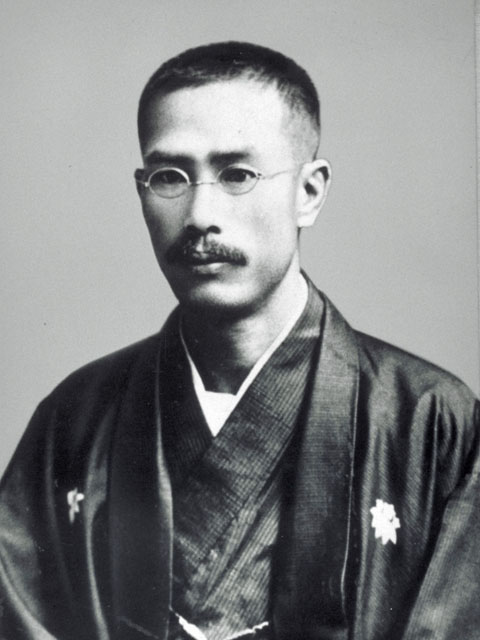
\includegraphics[height=0.9\textheight]{kawahigashi}\\[1em]
        \large{\FS 作~者~像}
    \end{figure}
\end{center}

\newpage

{\FS
    河东碧梧桐(1873—1937),日本爱媛县松山市人,本名秉五郎,又号如月、青桐、桐仙。父亲河东静溪是朱子派学者,在碧梧桐六岁时,就教他读四书五经。碧梧桐于一八八七年入伊予寻常中学,与高滨虚子是同级生。一八九〇年,碧梧桐十八岁时写了俳句集,请正冈子规批改。一八九一年,上东京投考第一高等学校落第。那年夏天,子规回乡省亲,他介绍高滨虚子到子规门下,学作俳句。一八九三年,考入第三高等学校,与虚子同住京都吉田町,宿舍称虚桐庵。次年秋,因学制改革,与虚子转学到仙台第二高等学校,不久与虚子一齐退学,同赴东京,帮助子规提倡俳句革新运动。于是成为子规门下双壁。一八九五年,子规病后,代替子规主持『日本俳句』栏,同年夏,陪子规的母亲去神户探望卧病的子规,并到日本新闻社去工作。翌年,退出日本新闻社,任『新声』杂志的俳句栏主选人。一八九七年,『杜鹃』杂志在松山创刊,负责选句,翌年该杂志移到东京之后,高滨虚子有病,由碧梧桐代替编辑。一九〇二年,搬到子规庵的附近上根岸去住,与子规更亲近,九月子规逝世,继任『日本俳句』的选句人。一九〇三年一月,他再度入日本新闻社,并为『温泉百句』问题,与虚子论战,从这时起,虚子和碧梧桐之间明显地出现了分歧。一九〇五年和一九〇六年,他两度召开「俳三昧」句会,参加者有小泽碧童、大须贺乙字等,专心致意于俳句,切磋琢磨。这时碧派的声势颇大。

    一九〇六年八月六日,经真言宗大谷句佛的资助,开始第一次周游全国。出发前,请高滨虚子接任『日本俳句』的选句工作。他一心渴望此次旅行能有助于使自己的俳境更加深广。翌年在旅次中,他的『新俳句研究谈』出版。一九〇九年四月第二次周游全国,在这一年又进一步阐发新倾向俳句论题。它的特色,可归纳为摆脱羁绊、追求写实、着意心理描写、发挥个性这几点。旅行结束后,他又提出无季自由律,打破俳句的十七音律与季语定型这两个要素,遂变俳句为一般的短诗了。碧梧桐及其对新倾向的俳句的主张,在近代俳句史上打下了划时期的印记,它带着急于开拓的冒进性,脱离了民族文化传统的基础,引起俳界的非议。

    一九二四年碧梧桐建立芜村研究会,为了研究芫村,翌年到与芜村有关的地方旅行,之后,出版了介绍芜村的俳句和绘画的『画人芜村』、『芜村研究』、『芜村新十一部集』、『芜村名句评释』等书。他或许受了赞赏芜村的子规的影响。关于自己的俳句作品和俳论,则有『碧梧桐句集』、『新倾向派俳句的研究』、『三千里』、『续三千里』和『回忆子规』等著作。他的俳风,给人以明快新颖的印象。此外,还编有『续春夏秋冬』、『日本俳句钞』等集子。本集中所选四十五首俳句,都是根据『新订俳句丛书·人与作品』第六卷(樱枫社1980年版)翻译的。
}

\newpage

\section{\FK 春}

\setcounter{haikucounter}{0}

\begin{haiku}
    {\FH ---}

    {\FK 三月三日因病终日闭居}

    {\FK 罗马春雨降,倚窗望天空。\footnote{\FT 未找到此句,碧梧桐文集里,同一标题是另一首俳句「{\FM ミモーザ買はしめて餓ゑて昼眠て}」。}}

    {\FT 注:一九二一年,作者经上海、新加坡,从马赛登陆到意大利罗马等地旅游。六月从巴黎到北欧。十一月到伦敦。十二月渡美,翌年一月回国。}
\end{haiku}

\begin{haiku}
    {\FH \ruby{楠}{くす}の芽に、日のさし風の、光るかな}

    {\FK 日照楠木芽,风吹亦有光。}

    {\FT 注:『楚辞』有「光风」的词儿。}
\end{haiku}

\begin{haiku}
    {\FH 春寒し、水田の上の、\ruby{根}{ね}さし雲。}

    {\FK 早春寒气临,水田上空云无根。}

    {\FT 注:俳人协会故会长大野林火说此句是暗示在悲剧中终了一生的碧梧桐的境涯。句带浪漫味,哀愁美。}
\end{haiku}

\begin{haiku}
    {\FH 曲すみし、\ruby{笛}{ふえ}の\ruby{余音}{よいん}や、春の月。}

    {\FK 横笛一曲终,余音绕春月。}
\end{haiku}

\begin{haiku}
    {\FH 蛇穴を、出でて石\ruby{垣}{がき}の、春の水。}

    {\FK 蛇出洞穴来,石垣春水漾。}

    {\FT 注:句用写生手法,表示敏锐的季节感。}
\end{haiku}

\begin{haiku}
    {\FH \ruby{桐}{きり}の木に、なく\ruby{鶯}{うぐいす}も、茶山哉}

    {\FK 黄莺桐树鸣,茶山多一景。}

    {\FT 注:茶山指春日晴朗时采茶的事,桐树飞来鸣莺,也算多一种景趣。}
\end{haiku}

\begin{haiku}
    {\FH 永き日や、羽\ruby{惜}{おし}む鷹の、嘴使ひ。}

    {\FK 春日迟迟,鹰嘴理毛羽。}

    {\FT 注:作者在此致力于「从平易外观直叙到内面事相与感想具象的描写」。}
\end{haiku}

\begin{haiku}
    {\FH 赤い椿白い椿と落ちにけり。}

    {\FK 红山茶,白山茶,叠地有落花。}

    {\FT 注:此句印象明瞭,如一幅油画,只见地上落下一簇红花,一簇白花,而其场所,使人联想起庭园或山路。这是多被引用、欣赏的名句。}
\end{haiku}

\begin{haiku}
    {\FH 桃咲くや、\ruby{湖}{ご}水のへりの、十個村。}

    {\FK 桃开花似锦,湖水周边十个村。}

    {\FT 注:桃是栽培在农村庭院的花木。此句写桃花开时,瞭望湖边十个村(小村)的艳丽景色。「十个村」用的是汉文。}
\end{haiku}

\section{\FK 夏}

\setcounter{haikucounter}{0}

\begin{haiku}
    {\FH 雪を渡りて、また\ruby{薫風}{くんぷう}の、\ruby{草花}{そうか}\ruby{踏}{ふ}む。}

    {\FK 才行积雪上,又踏熏风草花路。}

    {\FT 注:这里的草花,按『日本的山水』均属于高山植物。句写渡过残雪,又在夏天薰风中踏过花畦,显出爽快明朗、健康的情趣。这是作者在『续三千里』的旅途中,写立山(在富山县西南隅)顶上的即景句。}
\end{haiku}

\begin{haiku}
    {\FH パン屋が出来た、葉櫻の午の、風渡る。}

    {\FK 面包店铺已开业,午问吹渡叶樱风。}

    {\FT 注:叶樱,指樱花开谢后,即长满叶子的樱树。初夏的风一吹,樱树就闪着叶光。此句写郊区商业发达的景象。}
\end{haiku}

\begin{haiku}
    {\FH \ruby{愕然}{がくぜん}として、昼寝さめたる、一人かな。}

    {\FK 愕然昼寝醒,孑立一孤身。}

    {\FT 注:炎夏疲乏,多作午睡。「愕然」用的是汉文。}
\end{haiku}

\begin{haiku}
    {\FH 砲車過ぐる、\ruby{巷}{ちまた}の\ruby{塵}{ごみ}や、日の\ruby{盛}{さか}り。}

    {\FK 炮车驶向巷里过,夏日光中舞沙尘。}

    {\FT 注:此句用新词「炮车」,有时代感。}
\end{haiku}

\begin{haiku}
    {\FH 海楼の、涼しさ\ruby{終}{つ}ひの、別れかな。}

    {\FK 海楼凉气清,惜别此时情。}

    {\FT 注:作者开始「三千里」的旅行,从两国站来到稻毛寄宿于海边松林中的海气馆。门徒乙字、六花、观鱼、碧童等来相送,作此留别句。}
\end{haiku}

\begin{haiku}
    {\FH 馬独り、\ruby{忽}{こつ}と戻りぬ、飛ぶ蛍。}

    {\FK 马儿忽自归,流萤闪烁飞。}
\end{haiku}

\begin{haiku}
    {\FH \ruby{水鶏}{くいな}来し、夜明けて田水、満てるかな。}

    {\FK 水鸡来到黎明前,水淹满田间。}

    {\FT 注:水鸡,身茶褐色、脚长,栖息在芦丛中。黎明前和黄昏时发出象叩门一样的叫声,与「来到」的发音近似。}
\end{haiku}

\begin{haiku}
    {\FH \ruby{温泉}{ゆ}の宿に、馬の子\ruby{飼}{か}へり、\ruby{蠅}{はえ}の声。}

    {\FK 温泉宿舍喂小马,可厌苍蝇声。}

    {\FT 注:小马可爱,蝇声可厌,作者很技巧地把爱与憎凑在一起。}
\end{haiku}

\begin{haiku}
    {\FH 空をはさむ、蟹死にをるや、雲の峰。}

    {\FK 蟹死整钳空,炎天涌云峰。}

    {\FT 注:蟹可能指海蟹。它要钳取什么,终于未能钳着,作者有其寓意。云峰做为死蟹的背景。}
\end{haiku}

\begin{haiku}
    {\FH ---}

    {\FK 西光寺寄宿}

    {\FK 书籍放在桌台上,檐前蔷薇放白光。\footnote{\FT 未找到此句。}}
\end{haiku}

\section{\FK 秋}

\setcounter{haikucounter}{0}

\begin{haiku}
    {\FH 近作を、画室に掛くる、秋日影。}

    {\FK 画室悬近作,秋日光照来。}
\end{haiku}

\begin{haiku}
    {\FH 一軒家も、過ぎ落ちる風の、ままに行く。}

    {\FK 风急吹叶落,陆风过孤屋。}
\end{haiku}

\begin{haiku}
    {\FH 墓と見えて、十字架立つる、秋の山。}

    {\FK 十字架立秋山上,坟墓在望中。}

    {\FT 注:此句用新词「十字架」,带着近代化色彩。}
\end{haiku}

\begin{haiku}
    {\FH 天下知る、\ruby{藏書}{ぞうしょ}見に\ruby{来}{こ}ぬ、秋の晴れ}

    {\FK 藏书名传天下知,来求批览秋晴时。}
\end{haiku}

\begin{haiku}
    {\FH 大風に、傷みし樹々や、渡り鳥。}

    {\FK 大风伤万木,候鸟南归去。}
\end{haiku}

\begin{haiku}
    {\FH 鶴とんで、かえらず池の、水寒。}

    {\FK 萧萧池水寒,鹤飞去不还。}
\end{haiku}

\begin{haiku}
    {\FH 曳かれる牛が、辻でずっと見廻した、秋空だ。}

    {\FK 被牵耕牛停下步,十字路上凝望秋空。}

    {\FT 注:牛被牵走,是到市场呢,还是到屠场?牛也许感到事关自己的命运。此句共计二十三音(7、11、5),破了调,但有季语「秋空」。}
\end{haiku}

\begin{haiku}
    {\FH から松は、淋しき木なり、赤蜻蛉。}

    {\FK 落叶松寂静,红蜻蜓群舞无声。}

    {\FT 注:此句写晚秋萧瑟静寂的景趣。以落叶松为主,红蜻蜓作陪。俳人碧梧桐与诗人北原白秋的『落叶松』诗境,情感相通。}
\end{haiku}

\begin{haiku}
    {\FH 三日月や、この頃萩の、咲きこぼれ。}

    {\FK 新月刚刚出,胡枝子花零落。}
\end{haiku}

\begin{haiku}
    {\FH この道の、富士になり行く、\ruby{芒}{すすき}かな。}

    {\FK 路径向富士,茫茫狗尾草。}
\end{haiku}

\begin{haiku}
    {\FH 夜に入りて、\ruby{蕃椒}{とうがらし}\ruby{煮}{に}る、臺所。}

    {\FK 时已到夜晚,厨房煮辣椒。}

    {\FT 注:写生活琐事,句法平易,并无陈腐气。子规在『俳句』新派的一种倾向中举了这句。}
\end{haiku}

\begin{haiku}
    {\FH \ruby{芙蓉}{ふよう}見て立つうしろ灯るや。}

    {\FK 伫立看芙蓉,背后点亮灯。}

    {\FT 注:芙蓉是栽培在庭院中的花木,早上开花,傍晚凋萎。此时,室内点起了灯。芙蓉结束了一天的工作,灯火却刚刚点亮,此句写微妙的瞬间变化。}
\end{haiku}

\section{\FK 冬}

\setcounter{haikucounter}{0}

\begin{haiku}
    {\FH 火も置かず、独居の人と、夜長かな。}

    {\FK 夜长不备火,清冷独居人。}
\end{haiku}

\begin{haiku}
    {\FH 夜を寒み、人語聞えて、森の寺。}

    {\FK 寒夜闻人语,庵寺在林中。}
\end{haiku}

\begin{haiku}
    {\FH \ruby{我善坊}{がぜんぼう}に、車引き入れ、ふる霰。}

    {\FK 车入我善坊,玉霰落纷纷。}

    {\FT 注:车是明治时代的人力车,我善坊是谷间的一个町(行政区划,位于市、区之下)名。霰即常见于初冬时的雪珠。天一阴沉便一小粒一小粒地降落,又叫米雪。}
\end{haiku}

\begin{haiku}
    {\FH 芒枯れし、池に出づ\ruby{工場}{こうば}、さかる\ruby{音}{ね}を。}

    {\FK 漫步到枯芒池畔,风传来工厂噪声。}

    {\FT 注:枯芒是初冬季语,噪音据云可能是木材厂的锯声。}
\end{haiku}

\begin{haiku}
    {\FH 枯木原に、雪積んで居る、月夜かな。}

    {\FK 朦朦月夜,雪封枯木原野。}
\end{haiku}

\begin{haiku}
    {\FH 後宮の、夜半に雪折、聞えけり。}

    {\FK 雪重折枝声,后宫夜半闻。}
\end{haiku}

\begin{haiku}
    {\FH 軒落ちて、雪\ruby{窮}{きゅう}\ruby{巷}{こう}を、\ruby{塞}{ふさ}ぎけり。}

    {\FK 轩前积落雪,贫巷路不通。}

    {\FT 注:据云此句原文是汉语调,系明治俳句的一种特色。}
\end{haiku}

\begin{haiku}
    {\FH 寒林の、貧寺焼けたり、僧の留守。}

    {\FK 寒林贫寺火神来,僧人不知何处去。}
\end{haiku}

\begin{haiku}
    {\FH \ruby{木}{こ}\ruby{枯}{がらし}や、\ruby{谷}{や}中の道を、塔の下。}

    {\FK 大风吹落木,塔下谷中路。}

    {\FT 注:谷中指东京都台东区、上野公园的北部一带,多墓地、寺院和树林。子规的住地根岸离那儿不远。此句系碧梧桐走过那条风吹寒林、落叶飘飞的路时所作。}
\end{haiku}

\begin{haiku}
    {\FH 極月の、風雪\ruby{熊羆}{いうひ}、叫びけり。}

    {\FK 腊月风雪紧,熊罴吼叫声。}
\end{haiku}

\begin{haiku}
    {\FH 灯あかあかと、\ruby{会}{あわ}すれば、千鳥、鳴くといふ。}

    {\FK 会友华灯下,千鸟发鸣声。}

    {\FT 注:写会到意志相投的友人,感到欢欣,以千鸟叫声,作为伴奏。此句打破俳句五、七、五的定型,用六、五、三、五调。}
\end{haiku}

\section{\FK 无季}

\setcounter{haikucounter}{0}

\begin{haiku}
    {\FH 大戦に、\ruby{死所}{ししょ}を得ず\ruby{哀}{あわ}れ、野はかれて。}

    {\FK 读史}

    {\FK 大战未能得死所,悲叹原野尽荒芜。}
\end{haiku}

\begin{haiku}
    {\FH 故人こゝに、在りし遺物と、\ruby{新酒}{しんしゅ}かな。}

    {\FK 怀子规居士旧事}

    {\FK 往昔故人居此处,遗物新酒惹怀思。}
\end{haiku}

\begin{haiku}
    {\FH \ruby{汐}{しお}のよい\ruby{船}{ふな}\ruby{脚}{あし}を瀬戸の\ruby{鷗}{かもめ}は鷗づれ。}

    {\FK 船行潮水好,濑户鸥群竞逐飞。}
\end{haiku}

\chapter[{\FM 高浜虚子}]{\FM \ruby{高}{たか}\ruby{浜}{はま}\ruby{虚}{きょ}\ruby{子}{し}}

\begin{center}
    \begin{figure}
        \centering
        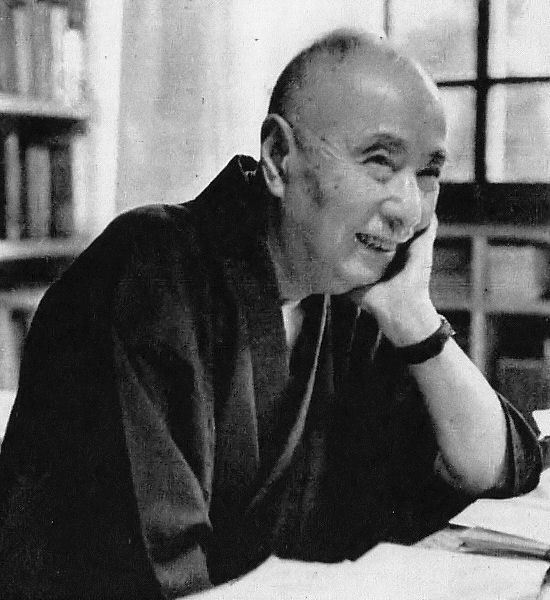
\includegraphics[width=\textwidth]{takahama}\\[1em]
        \large{\FS 作~者~像}
    \end{figure}
\end{center}

\newpage

{\FS
    高滨虚子(1874—1959)生于爱媛县松山市长町新町,本名清。父亲是松山藩士池内庄四郎。废藩设县后,全家搬到风早郡柳原村西下务农。西下家乡风光美好,虚子的童年就在那里度过。父亲爱好谣曲、和歌,母亲也爱好文艺,给虚子很深的影响,从而日后致志于文学工作。八岁时,因四个哥哥均不愿务农,举家又迁回到松山。九岁时,祖母病故,出嗣到祖母家,改姓高滨。一八九一年三月父亲逝世。同年五月伊予寻常中学级友河东碧梧桐(松山人)介绍高滨虚子一起向同乡先辈正冈子规学作俳句。子规以他的本名「清」的谐音,在信里称他为虚子,从此就以虚子作为俳号了。一八九四年虚子与碧梧桐到东京,鼓吹子规所号召的俳句改革主张。翌年冬子规在上野道灌山疗养时,恳请虚子担任俳句革新运动的后继人,但虚子顾虑羁绊太多,婉言辞谢。

    一八九八年一月,『杜鹃』杂志经柳原极堂之手在松山发刊,但因经营不善,由虚子接过来。翌年听子规的建议迁移到东京出版,虚子任发行人,遂面目一新,并培养了不少人才。该刊表现了明治、大正、昭和三代的俳句史的大观。虚子一生的文学活动与『杜鹃』的关系十分密切。子规死后,夏目漱石也给予支持,他的名著『我是猫』,在该刊连载,获得好评。因此刺激了虚子,他也热中于小说的写作,仅一九〇七年一年之内,就在『杜鹃』上发表了『风流忏悔』、『斑鸠故事』、『大内旅馆』等作品。翌年,又将『俳谐师』一作在『国民新闻』上连载。晚年在小诸又写小说『虹』,川端康成给予很高的评价,说虚子是明治以后在艺术上最臻于圆熟的一个人。

    一九〇八年,河东碧梧桐开始提倡俳句新倾向。一九一三年虚子回到俳坛时,写下如下宣言性的俳句:「斗心已抱定,独立丘上迎春风。」他反对新倾向运动,因该运动主张破坏俳句固有的定型,并提倡季题无用论,有发展到无季俳句与自由律的趋势。虚子有自己的俳论,自认为是守旧派。他要维持俳句的结构,说季语不能弃置,与从青年时代就很亲密的碧梧桐对立。在创作方法上,他继承了子规那种客观写生的主张。也就是说,要精细地观察事物,如实地予以描写。题材方面,他主张吟咏花鸟风月,注重自然美。他认为俳句是叙景诗:「俳句的目的,在于吟咏风月。」又说俳句是平俗的诗,俳句是日常的诗……望峻岭、渡大泽,这里有俳句;目见耳闻处,那里有俳句;心感神通处,那里有俳句;太阳出没,寒暑往来,为俳句的根干。他还强调,心情感到悲与喜,应该描写那引起感受的景物。他的注重自然美和日本文艺传统,是有所联系的。他终年八十六,作句又勤,句集浩繁,有独特的风格,有的秀逸轻妙,有的平易纯朴,为广大读者所欢迎。他的文学活动,反映了自己的思想感情,也反映了时代和社会某个角度的情况。由于他多年来在日本俳句等方面的建树,一九五四年十一月获得日本政府颁给的文化勋章。本集中所选一〇八首俳句,都是根据『高滨虚子全集』(共16卷,每日新闻社1974—1975年版)翻译的。
}

\newpage

\section{\FK 新年}

\setcounter{haikucounter}{0}

\begin{haiku}
    {\FH \ruby{去年}{こぞ}\ruby{今年}{ことし}、\ruby{貫}{つらぬ}く棒の、\ruby{如}{ごと}きもの。}

    {\FK 去年与今年,相连如木棍。}

    {\FT 注:这是一九五〇年新年广播的录音句。「去年今年」是俳句的新年季语。作者晚年常说要平凡,他把岁月比作单调的木棍,也可以说是达人达观吧。}
\end{haiku}

\begin{haiku}
    {\FH 手毬唄、悲しきことを、うつくしく。}

    {\FK 悲切手球歌,听来觉得美好。}
\end{haiku}

\begin{haiku}
    {\FH \ruby{琴}{きん}\ruby{棋}{き}\ruby{書}{しょ}\ruby{畫}{が}、松の内なる、遊びかな。}

    {\FK 遣兴松房里,琴棋书画多清趣。}
\end{haiku}

\section{\FK 春}

\setcounter{haikucounter}{0}

\begin{haiku}
    {\FH 春惜む、命惜むに、\ruby{異}{ことな}らず。}

    {\FK 惜春无异惜生命。}

    {\FT 注:一九五〇年作于御苑内霜锦亭举行句会时。}
\end{haiku}

\begin{haiku}
    {\FH 遠ざけて、引寄せもする、春火桶。}

    {\FK 摆出火钵子,春寒闲话时。}
\end{haiku}

\begin{haiku}
    {\FH \ruby{踏}{とう}\ruby{青}{せい}や、古き石\ruby{階}{ばし}、あるばかり。}

    {\FK 踏青呀,只在古旧石阶旁。}

    {\FT 注:踏青是中国的旧俗,三月三日行事,又称踏春,清末梁鼎芬『卜算子』有「只好明年再踏春」之句。}
\end{haiku}

\begin{haiku}
    {\FH 橋に立てば、春水我に、向って来。}

    {\FK 伫立桥头上,春水向我涌来。}
\end{haiku}

\begin{haiku}
    {\FH \ruby{春灯}{しゅんとう}の、下に我あり、\ruby{汝}{いまし}あり。}

    {\FK 华灯春宵里,有我也有你。}
\end{haiku}

\begin{haiku}
    {\FH 春灯、鏡の中の、春灯。}

    {\FK 春灯啊,镜里的春灯。}

    {\FT 注:以反映的手法托出春灯的美。}
\end{haiku}

\begin{haiku}
    {\FH 春潮と、いへば必ず、門司を思ふ。}

    {\FK 提起春潮事,当然想念门司。}

    {\FT 注:春时潮色变作浅蓝,看潮色知道春到来,心情愉快。门司是接联玄海滩与濑户内海的城市,潮景明朗。}
\end{haiku}

\begin{haiku}
    {\FH 春雨に、傘を借りたる、別れかな。}

    {\FK 一八九六年别漱石}

    {\FK 绵绵春雨时,借伞告别离。}
\end{haiku}

\begin{haiku}
    {\FH 思ひ川、渡ればまたも、花の雨。}

    {\FK 渡入思川去,又是花雨天。}

    {\FT 注:思川是地名。}
\end{haiku}

\begin{haiku}
    {\FH 春の山、\ruby{屍}{かばね}を埋めて、\ruby{空}{むな}しかり。}

    {\FK 春山泥土埋尸骨,生前功罪尽虚空。}

    {\FT 注:句意是说春山的草木花鸟仍在,而人的生前是非得失已成一场空。这是凭吊一代之雄源赖朝的。虚子作此句六天后即病逝,也与赖朝一样埋入土中。}
\end{haiku}

\begin{haiku}
    {\FH 独り句の、推敲をして、遅き日を。}

    {\FK 句佛师十七回忌追忆}

    {\FK 春日迟迟,独自推敲句子。}

    {\FT 注:这句是纪念真言宗大谷句佛氏忌辰,写在明信片上的绝笔。}
\end{haiku}

\begin{haiku}
    {\FH 窓外の、風塵春の、行かんとす。}

    {\FK 窗外风尘起,春将归去时。}
\end{haiku}

\begin{haiku}
    {\FH 春風や、\ruby{闘志}{とし}いだきて、丘に立つ。}

    {\FK 斗心已抱定,独立丘上迎春风。}

    {\FT 注:这是一九一三年作者四十岁上回归俳坛时的宣言句。后于一九五〇年又有「斗心尚在见春风」的吟句。}
\end{haiku}

\begin{haiku}
    {\FH ---}

    {\FK 莎士比亚菩提寺}

    {\FK 春日透过花玻璃,照射棺木上。\footnote{\FT 未找到此句。}}
\end{haiku}

\begin{haiku}
    {\FH ---}

    {\FK 漫步庭院里,木屐印春泥。\footnote{\FT 未找到此句。}}
\end{haiku}

\begin{haiku}
    {\FH 楊貴妃、という香水の、ありや無しや}

    {\FK 佳丽杨贵妃,有无点香水?}
\end{haiku}

\begin{haiku}
    {\FH ---}

    {\FK 柏林日本人句会}

    {\FK 主妇脸颊上,小猫脚爪痕。\footnote{\FT 未找到此句。}}
\end{haiku}

\begin{haiku}
    {\FH 鶯の、声の大きく、静かさよ。}

    {\FK 群鸟叫声逐渐高,终于静悄悄。}

    {\FT 注:这也是一种写生法,不用眼睛,而用耳朵。此句是时间艺术的表示。}
\end{haiku}

\begin{haiku}
    {\FH 穴を出る、蛇を見て居る、鴉かな。}

    {\FK 乌鸦看着蛇出洞。}
\end{haiku}

\begin{haiku}
    {\FH 江上の、燕は\ruby{緩}{ゆる}く、ボート\ruby{迅}{はや}し。}

    {\FK 燕子江天缓缓飞,船行何迅速。}
\end{haiku}

\begin{haiku}
    {\FH 鶯や、文字も知らずに、歌心。}

    {\FK 黄莺不识文字,却有歌吟的心。}
\end{haiku}

\begin{haiku}
    {\FH 蝶飛や、蘇山人の魂、遊ぶらん。}

    {\FK 飞蝶悠悠,岂是苏山人魂游。}

    {\FT 注:苏山人是作者的俳友,见正冈子规「春雨霏霏」句的注释。}
\end{haiku}

\begin{haiku}
    {\FH ---}

    {\FK 门前两亩桑,好把蚕来养。\footnote{\FT 未找到此句。}}
\end{haiku}

\begin{haiku}
    {\FH \ruby{海女}{あま}とても、\ruby{陸}{くが}こそよけれ、桃の花。}

    {\FK 渔女登上陆地,恍似桃花艳丽。}

    {\FT 注:一九四八年虚子游览三重县志摩时,看到外海渔女潜水采贝的作业,即作此句。操渔女作业的,多从少女时开始,她们登陆休息时焚火取暖,吃饭笑谈,也有给婴孩喂奶者。作者为渔女表示祝福之意,同时,又产生象桃花报南国之春的美感。}
\end{haiku}

\begin{haiku}
    {\FH 山居杉に、\ruby{親}{した}しめば、\ruby{連翹}{れんぎょう}野に恋し}

    {\FK 山居爱杉树,又恋连翘野原。}
\end{haiku}

\begin{haiku}
    {\FH 花見にと、馬に\ruby{鞍}{くら}置く、心あり。}

    {\FK 马背挂雕鞍,神往到花前。}

    {\FT 注:此句取材谣曲『马挂鞍』。花即樱花。}
\end{haiku}

\begin{haiku}
    {\FH 倫敦の、\ruby{春草}{しゅんそう}を踏む、我が草履。}

    {\FK 我的芒鞋哟,踩着伦敦的春草。}

    {\FT 注:作者旅欧时,穿和服与草鞋,是引人注目的。}
\end{haiku}

\begin{haiku}
    {\FH 初蝶\ruby{来}{く}、何色と\ruby{問}{と}ふ、\ruby{黄}{き}と答ふ。}

    {\FK 蝴蝶翩翩新到来,问何颜色答说黄。}

    {\FT 注:在这首俳句里面,有如闻其声的来、问、答三段对话,黄是三月间的花色。这是虚子作于信州小诸的名句。}
\end{haiku}

\begin{haiku}
    {\FH 一つ根に、離れ\ruby{浮}{う}く葉や、春の水。}

    {\FK 荇藻飘浮春水面,两叶分离根一条。}

    {\FT 注:这是写生的典型手法的例句。}
\end{haiku}

\begin{haiku}
    {\FH 鎌倉の、古き土より、牡丹の\ruby{芽}{め}。}

    {\FK 镰仓故土上,吐出牡丹芽。}
\end{haiku}

\begin{haiku}
    {\FH ---}

    {\FK 伫立花前不见花。\footnote{\FT 未找到此句。}}
\end{haiku}

\begin{haiku}
    {\FH 花散るや、鈍な鴉の、翅あたり。}

    {\FK 樱花瓣飘散,落在乌鸦钝翅膀。}

    {\FT 注:樱花的白瓣和乌鸦的黑翅膀,形成鲜明的对照,显出古典美。使人联想到李商隐的诗句「紫鸾不肯舞,满翅蓬山雪」(见『海上谣』)。描写白雪落在紫鸾的翅膀上,当各有其讽托之意。}
\end{haiku}

\begin{haiku}
    {\FH 散る花を、悼む心も、\ruby{慌}{あわただ}し。}

    {\FK 哀花谢落心零乱。}

    {\FT 注:一九四一年四月二十一日虚子哀悼维子郎逝世句。}
\end{haiku}

\begin{haiku}
    {\FH 此の谷の、梅の\ruby{遅速}{ちそく}を、獨り\ruby{占}{し}む}

    {\FK 不管梅开快与慢,独占此谷间。}
\end{haiku}

\begin{haiku}
    {\FH 金堂の、扉を\ruby{叩}{たた}く、木の芽風。}

    {\FK 树芽风,敲打金堂门。}
\end{haiku}

\begin{haiku}
    {\FH ---}

    {\FK 漂动急湍里,荇菜生机旺。\footnote{\FT 未找到此句。}}
\end{haiku}

\begin{haiku}
    {\FH \ruby{自}{みずか}ら草といい\ruby{芳草}{ほうそう}といわず。}

    {\FK 祝『草』三十五周年纪念}

    {\FK 自云是小草,不愿称瑶香。}
\end{haiku}

\section{\FK 夏}

\setcounter{haikucounter}{0}

\begin{haiku}
    {\FH 虹立ちて、\ruby{忽}{たちま}ち君の、\ruby{在}{あ}る\ruby{如}{ごと}し。}

    {\FK 长虹挂彩,忽想如君在。}
\end{haiku}

\begin{haiku}
    {\FH 虹消えて、忽ち君の、\ruby{無}{な}き如し。}

    {\FK 彩虹淌逝,忽想如君去。}

    {\FT 注:虚子旅居小诸,看见彩虹挂在浅间山顶,一九四四年十一月七日,在明信片上写下这两句给住在福井县的女弟子森田爱子。后用在他的小说『虹』的末尾。}
\end{haiku}

\begin{haiku}
    {\FH 夕立や、ぬれて戻りて、欄に\ruby{倚}{よ}る。}

    {\FK 骤雨身淋湿,归来独倚栏。}

    {\FT 注:此句系陪送正冈子规到须磨疗养院后所作。}
\end{haiku}

\begin{haiku}
    {\FH 夕立や、森を出で来る、馬車一つ。}

    {\FK 黄昏骤雨降,马车一驾出林来。}
\end{haiku}

\begin{haiku}
    {\FH 夏海や一帆の又見え来る。}

    {\FK 长夏海面上,又见风帆一叶来。}
\end{haiku}

\begin{haiku}
    {\FH 晩涼に、池の\ruby{萍}{うきくさ}、皆動く。}

    {\FK 一阵晚凉风,满池萍叶动。}

    {\FT 注:「晚凉」用汉语。白居易有「绿树阴前逐晚凉」句。}
\end{haiku}

\begin{haiku}
    {\FH 夏潮の、今\ruby{退}{そ}く平家、\ruby{亡}{ほろ}ぶ時も。}

    {\FK 夏潮今退去,平家灭亡时。}

    {\FT 注:这是咏史句。源义经在坛浦利用夏潮,指挥军船迫近平家的军船,瞬息之间决定了胜利。现在门司布刈神社有此句碑。}
\end{haiku}

\begin{haiku}
    {\FH 立山の、其連峰の、雪解水。}

    {\FK 悼下村为山}

    {\FK 立山巉岩上,夏雪正消溶。}
\end{haiku}

\begin{haiku}
    {\FH 静に居、\ruby{団扇}{うち}の風も、たまに好し。}

    {\FK 静静听说笑,悠悠团扇摇。}
\end{haiku}

\begin{haiku}
    {\FH ---}

    {\FK 芭蕉洒了水,卷叶冲上天。\footnote{\FT 未找到此句。}}
\end{haiku}

\begin{haiku}
    {\FH 夕嵐、青\ruby{鷺}{さぎ}吹き去って、高楼に灯。}

    {\FK 青鹭已随晚风去,高楼犹有灯火明。}

    {\FT 注:青鹭是大型鹭鸟,背苍灰色,故名。成群地在水边的树上作巢,喜在清凉的水中伫立。}
\end{haiku}

\begin{haiku}
    {\FH 蜘蛛に\ruby{生}{あ}れ、\ruby{網}{あみ}をかけねば、ならぬかな。}

    {\FK 生为蜘蛛,就该结网啊!}

    {\FT 注:这种意识形态,也是一种人生论。}
\end{haiku}

\begin{haiku}
    {\FH 蜘蛛網を、張るが如くに、我もあるか。}

    {\FK 象蜘蛛结网,我也是吗?}

    {\FT 注:一种人生论,在俳句这小体裁单纯地表现出来。}
\end{haiku}

\begin{haiku}
    {\FH 夏の蝶、日かげ日なたと、飛びにけり。}

    {\FK 夏天蝴蝶飞翔,向阴又向阳。}
\end{haiku}

\begin{haiku}
    {\FH 山国の、蝶をあらしと、思はずや。}

    {\FK 真没想到呀,搅乱了山区蝴蝶!}

    {\FT 注:一九四五年五月虚子沿着浅间山斜坡的田野路行走时,看见路两旁开着豌豆花,而蝴蝶群却飞得很慌乱,原来是被美军大轰炸吓的。这是对同行人顺口吟出之句,为代表作之一。}
\end{haiku}

\begin{haiku}
    {\FH 夏蝶の、つと落ち\ruby{来}{きた}り,とび\ruby{翔}{かけ}り。}

    {\FK 嬉戏落花地,蝴蝶追逐蝴蝶。}
\end{haiku}

\begin{haiku}
    {\FH \ruby{金}{こ}\ruby{亀子}{がねむし}、\ruby{擲}{なげう}つ闇の、深さかな。}

    {\FK 扔掉的金龟子,飞入黑暗深处。}

    {\FT 注:金龟子,夏天甲虫,白天藏在草木荫处,夜间出来绕着灯火飞动。}
\end{haiku}

\begin{haiku}
    {\FH ---}

    {\FK 萤火虫受了伤,跌落水面上。\footnote{\FT 未找到此句。}}
\end{haiku}

\begin{haiku}
    {\FH \ruby{主客}{しゅかく}\ruby{閑話}{かんわ}、ででむし竹を、上るなり。}

    {\FK 宾主在谈天,蜗牛爬上竹竿。}
\end{haiku}

\begin{haiku}
    {\FH 我を見て、\ruby{舌}{した}を出したる、大\ruby{蜥蜴}{とかげ}。}

    {\FK 这只大蜥蜴,吐出舌尖看着我。}

    {\FT 注:大蜥蜴吐舌的怪模样,使作者苦笑地对着它。}
\end{haiku}

\begin{haiku}
    {\FH 山を出でて、山に入る月や、蚊帳の外。}

    {\FK 蚊帐外,月儿出山又入山。}
\end{haiku}

\begin{haiku}
    {\FH 蚊帳越しに、\ruby{薬}{やく}煮る母を、かなしみつ。}

    {\FK 掀开蚊帐,愁看煎药的母亲。}
\end{haiku}

\begin{haiku}
    {\FH 薔薇剪って、短き詩をぞ、作りける。}

    {\FK 修剪蔷薇时,兴起吟短诗。}
\end{haiku}

\begin{haiku}
    {\FH \ruby{藻}{も}の花を、かづいて出でし、泳ぎかな。}

    {\FK 戴上水藻花,出去游泳啦。}

    {\FT 注:藻草生在湖泊水底,绿叶蹿出水面。夏天,叶间绽开淡绿、黄、白等色的花。}
\end{haiku}

\begin{haiku}
    {\FH 牡丹の、一弁落ちぬ、俳\ruby{諧}{かい}史。}

    {\FK 俳谐史上,掉落牡丹一瓣。}

    {\FT 注:此句是追悼俳人松本氏的逝世。因松本氏的人品、句品均佳,作者把他比作白牡丹的一瓣。}
\end{haiku}

\begin{haiku}
    {\FH 夕顔の、花に涙を、流すかな。}

    {\FK 子规病笃}

    {\FK 滴滴泪水,落在瓠瓜花蕊。}

    {\FT 注:此句作于一九〇一年二七月。瓠瓜,日本称夕颜,原产于美国\footnote{{\FT 瓠瓜和夕颜实为葫芦,学名} \textit{Lagenaria siceraria}{\FT ,原产于非洲。}}。茎叶有软毛,晚间开白花,翌晨即凋萎。子规院子里,有个作药用的瓠瓜棚,故这么说。}
\end{haiku}

\section{\FK 秋}

\setcounter{haikucounter}{0}

\begin{haiku}
    {\FH 手で顔を、撫づれば鼻の、冷たさよ。}

    {\FK 伸手一摸脸,鼻子好凉呦。}

    {\FT 注:句自然浅白,又稍带幽默感。这是虚子的另一种句式。}
\end{haiku}

\begin{haiku}
    {\FH 秋風や、眼中のもの、皆俳句。}

    {\FK 秋风吹拂凉,眼中万物皆诗章。}
\end{haiku}

\begin{haiku}
    {\FH 霧の中に、蓑の人現れ、又隠れぬ。}

    {\FK 雾里蓑衣人,乍现又乍隐。}
\end{haiku}

\begin{haiku}
    {\FH 百花園、野分の跡を、見に来たり。}

    {\FK 来到百花园里,巡视大风过后痕迹。}
\end{haiku}

\begin{haiku}
    {\FH ---}

    {\FK 银河无踪影,只有月亮和昴星。\footnote{\FT 未找到此句。}}
\end{haiku}

\begin{haiku}
    {\FH 秋の雲、\ruby{太虚}{たいきょ}の風に、乗りにけり。}

    {\FK 秋空一片云,悠闲漫步行。}
\end{haiku}

\begin{haiku}
    {\FH ---}

    {\FK 大圆月,印在门帘上。\footnote{\FT 未找到此句。}}
\end{haiku}

\begin{haiku}
    {\FH これよりは、山陰道の、月暗し。}

    {\FK 悼山本村家}

    {\FK 山阴道上,今后月暗淡。}
\end{haiku}

\begin{haiku}
    {\FH 草の露、三千人の、涙かな。}

    {\FK 子规七七忌追悼句会}

    {\FK 草上露,三千人的泪珠。}
\end{haiku}

\begin{haiku}
    {\FH 虚子一人、銀河と共に、西へ行く。}

    {\FK 虚子单身,随银河西行去。}

    {\FT 注:此句有向往西方净土的佛家思想。作者还有「寝中寂静,唯有银河流水声」的想象句。}
\end{haiku}

\begin{haiku}
    {\FH \ruby{仲麿}{なかまろ}の、舟は波間や、天の川。}

    {\FK 浪里晁衡船,天河腾翻。}

    {\FT 注:此是怀古句。日本晁衡从长安回国途中,在海上遇大风浪,展转折回长安。李白有诗怀念他,}
\end{haiku}

\begin{haiku}
    {\FH 船に乗れば、陸\ruby{情}{なさ}けあり、暮の秋。}

    {\FK 暮秋扬帆去,我念陆地情。}

    {\FT 注:一九一八年十月为纪念亡兄逝世三周年,在回乡的途中所作。虽说客观写生,却是主观抒情句。}
\end{haiku}

\begin{haiku}
    {\FH \ruby{病}{わくら}葉や、大地に何の、病ある。}

    {\FK 大地染何疾?病叶尽飘零。}
\end{haiku}

\begin{haiku}
    {\FH \ruby{爛}{らん}々と、昼の星見え、\ruby{菌}{きの}生え。}

    {\FK 火星何灿烂,蘑菇妖艳生。}

    {\FT 注:原文「昼星」,依山本健吉作「火星」解,故照译。此句写秋空星光灿烂,而地下的蘑菇红黄妖艳,天上地下,不同色彩,形成鲜明对照。}
\end{haiku}

\begin{haiku}
    {\FH \ruby{来}{こ}ん秋を、再び期して、別れけり。}

    {\FK 此刻一为别,来秋期再会。}
\end{haiku}

\begin{haiku}
    {\FH \ruby{落花生}{らっかせい}、喰ひつゝ読むや、罪と罰。}

    {\FK 边吃花生边阅读,『罪与罚』那本书。}
\end{haiku}

\begin{haiku}
    {\FH 彼一語、我一語秋、深みかも。}

    {\FK 他一言,我一语,不觉秋已深。}

    {\FT 注:写在宾主愉快交谈时,室外日己斜,落叶也飘舞了,这是寄喻人生到了秋深的时节。}
\end{haiku}

\begin{haiku}
    {\FH 月を思い、人を思ひて、須磨にあり。}

    {\FK 客居须磨浦,怀月又怀人。}

    {\FT 注:须磨在神户西部南海岸。『源氏物语』的主人公光源氏曾被谪在此,这里的月亮照过历史上多少豪杰。虚子于五十多年前陪送正冈子规到此地疗养,曾一起赏月,不禁引起追怀。}
\end{haiku}

\begin{haiku}
    {\FH 落葉降り、やがて雪降り、霰降り。}

    {\FK 落叶飘下,接着雪飘下,霰飘下。}

    {\FT 注:此句写自然规律,也有人生飘忽之感。}
\end{haiku}

\begin{haiku}
    {\FH \ruby{案}{あん}\ruby{山}{ざん}\ruby{子}{し}、我に向ひて、問答す。}

    {\FK 稻草人向我搭话。}
\end{haiku}

\begin{haiku}
    {\FH ひらひらと、\ruby{釣}{つ}られて淋し、今年\ruby{鯊}{はぜ}。}

    {\FK 江中木桩上,独坐钓鲨鱼\footnote{\FT 这里的鲨鱼实际是虾虎鱼。}。}
\end{haiku}

\begin{haiku}
    {\FH 胸出して、\ruby{鳩}{はと}のぼり來る、落葉坂。}

    {\FK 鸽子胸挺挺,登上落叶坡。}
\end{haiku}

\begin{haiku}
    {\FH わが\ruby{庵}{いお}の、椿に\ruby{鵯}{ひよ}の、来る日課。}

    {\FK 我家山茶树一棵,鹎鸟探花当日课。}

    {\FT 注:鹎系鸣禽类,形似画眉,善飞翔,飞时一上一下波状地向前。}
\end{haiku}

\begin{haiku}
    {\FH この松の、下にたゝすめは、露のわ\ruby{連}{つら}。}

    {\FK 伫立此松下,露之中。}

    {\FT 注:在风早村西下家乡的屋子旁边,有一棵老松树,虚子幼时常在松树下玩耍。隔了三十多年回乡再看时,老松依然耸立,难兔有所追怀。表示人在露中,从露又联想到泪,有点感伤。}
\end{haiku}

\begin{haiku}
    {\FH 桐一葉、日当りながら、落ちにけり。}

    {\FK 桐树日光照,枝梢一叶飘。}

    {\FT 注:写出天地幽玄的信息,一叶落而知秋。虚子名句之一。}
\end{haiku}

\begin{haiku}
    {\FH ---}

    {\FK 大江两岸,芦苇割掉了吗?\footnote{\FT 未找到此句。}}
\end{haiku}

\begin{haiku}
    {\FH ---}

    {\FK 荷残柳败城池在。\footnote{\FT 未找到此句。}}
\end{haiku}

\begin{haiku}
    {\FH ---}

    {\FK 苹果未吃完,放在手册上。\footnote{\FT 未找到此句。}}
\end{haiku}

\begin{haiku}
    {\FH 枯菊の、色\ruby{尚}{なお}\ruby{存}{そん}す、霜の庭。}

    {\FK 菊残色尚美,犹立风霜庭院里。}
\end{haiku}

\section{\FK 冬}

\setcounter{haikucounter}{0}

\begin{haiku}
    {\FH 遠山に、日の当りたる、枯野かな。}

    {\FK 举目远山前,薄日照荒原。}

    {\FT 注:这是早期在虚子庵例上作的俳句。冬天的日光令人感到温暖。此句是作者喜爱的代表作之一。}
\end{haiku}

\begin{haiku}
    {\FH ---}

    {\FK 携伞向前行,枯野听雨声。\footnote{\FT 未找到此句。}}
\end{haiku}

\begin{haiku}
    {\FH ---}

    {\FK 寒夜出当铺,仰观岁暮月。\footnote{\FT 未找到此句。}}
\end{haiku}

\begin{haiku}
    {\FH 眠れねば、いろいろの智慧、夜半の冬。}

    {\FK 醒来冬夜半,慧想起联翩。}
\end{haiku}

\begin{haiku}
    {\FH 二行書き、一行\ruby{消}{け}すや、寒灯下。}

    {\FK 寒灯下,写两行删一行。}
\end{haiku}

\begin{haiku}
    {\FH ---}

    {\FK 就在寒潮里,河豚毒洗去。\footnote{\FT 未找到此句。}}
\end{haiku}

\begin{haiku}
    {\FH \ruby{鳰}{にお}がゐて、鳰の海とは、昔より。}

    {\FK 浮游䴙䴘在,自古便称䴙䴘海。}

    {\FT 注:琵琶湖的湖面有点点的水鸟䴙䴘,故称䴙䴘海。『万叶集』中有柿本人麻吕的短歌:「䴙䴘海波涌,黄昏千鸟鸣,汝鸣吾有感,思古发幽情。」松尾芭蕉有俳句:「四方飘下花雪来,尽归䴙䴘海。」一九三九年秋,虚子在琵琶湖饭店作此句,抒发怀古之情。}
\end{haiku}

\begin{haiku}
    {\FH 鴨の中の、一つの鴨を、見てゐたり。}

    {\FK 在鸭群里,单看着一只。}
\end{haiku}

\begin{haiku}
    {\FH 水鳥の、夜半の羽音や、あまたたび。}

    {\FK 时已到深更,水鸟屡发拍翅声。}

    {\FT 注:写大静中小动的声音,稍显出幽玄感。}
\end{haiku}

\begin{haiku}
    {\FH 鳴くたびに、枝踏みゆるゝ、寒鴉。}

    {\FK 寒鸦鸣叫时,踏跳着树枝。}
\end{haiku}

\begin{haiku}
    {\FH 大根を、\ruby{鷲}{わし}づかみにし、五六本。}

    {\FK 大鹫抓萝卜,五六根。}
\end{haiku}

\begin{haiku}
    {\FH 流れ行く、大根の葉の、早さかな。}

    {\FK 川上萝卜叶,急速漂流去。}

    {\FT 注:作者在小川的桥上,看见水上萝卜叶很快地流去,就照实况吟出那瞬间的情趣。}
\end{haiku}

\begin{haiku}
    {\FH ---}

    {\FK 离离浦岛草,霜中一夜即衰老。\footnote{\FT 未找到此句。}}
\end{haiku}

\chapter[{\FM 水原秋櫻子}]{\FM \ruby{水}{みず}\ruby{原}{はら}\ruby{秋}{しゅう}\ruby{櫻}{おう}\ruby{子}{し}}

\begin{center}
    \begin{figure}
        \centering
        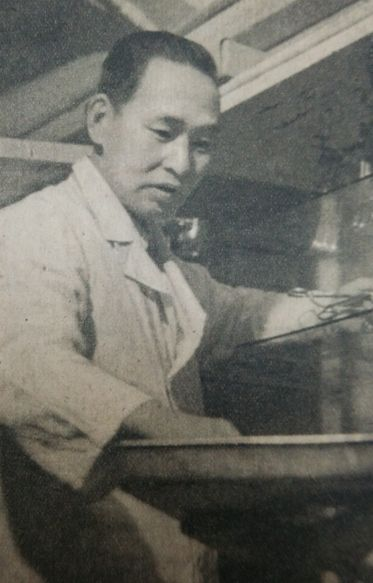
\includegraphics[height=0.9\textheight]{mizuhara}\\[1em]
        \large{\FS 作~者~像}
    \end{figure}
\end{center}

\newpage

{\FS
    水原秋樱子(1892—1982),生于东京神田猿乐町,本名丰,别号喜雨亭。父熊三郎,母治子,秋樱子是长子。学历是东京高师附属小学校、德国学协会中学,二十岁入第一高等学校。这时爱读歌集。一九一八年毕业于东京帝国大学医学部。在校时吟咏短歌。后获得医学博士学位,并任昭和医专教授。他经营过妇产科病院,还在宫内省侍医寮任过职。一九一八年他接触高滨虚子的俳句论文,对俳句发生兴趣,遂购读『杜鹊』杂志。翌年在血清化学教室的先辈绪方春桐的劝告下开始作句,入了树芽会,俳号静夏。因该会领导人南仙卧、野村喜舟等的缘故,出席『涩柿』俳句会,不满意于松根东洋城对写生法的指导,改向『杜鹃』杂志投稿,在例会上初次见高滨虚子。那时期,医学先辈宇都野研办『朝光』歌志,劝秋樱子向窪田空穗学习短歌,作歌入选。一九二二年与山口誓子、日野草城、富安风生、高野素十、山口青邨等建立东大俳句会,给『杜鹃』吹入一股新风。由于秋樱子、誓子、素十、青邨这四个活跃的人物,名字用拉丁文拼出来的话,字头都是S,昭和初期的『杜鹃』杂志遂出现了四S时代。

    一九二二年,秋樱子加入佐佐木绫华主宰的『破魔弓』,被推选为选者。一九二八年七月该杂志改名为『马醉木』,长期由秋樱子主持职务。关东大地震后,秋樱子不再写短歌,致力于俳句,到全国名胜旅游,感兴作句。此后,反对『杜鹃』上的那些陷于烦琐描写的客观写生。一九三一年十月,在『马醉木』发表名文『自然的真与文艺的真』,脱离了『杜鹃』杂志社。他认为自然的真不等于艺术上的真,自然的真不过是一种素材,需要作者琢磨,主观的沉浸,获得艺术的旨趣,而达到自由抒情的目的。他既不赞同作句如实的客观写生,也不愿意停留在花鸟的吟咏上。要求清新活泼,导入短歌抒情表现,树立主观写生。

    对连作俳句的倡导后来引起了新兴俳句运动,环绕着季题存废问题,俳坛上展开了争论。秋樱子批判无季和口语化的倾向,坚持有季,定型,使用文语。一九六二年五月就任俳人协会会长、一九七八年任名誉会长。一九六四年获得日本艺术院奖,一九六六年被推选为日本艺术院会员。

    他的著作甚丰,包括『葛饰』、『新树』、『秋苑』、『浮叶抄』等句集,俳论、随笔、纪行、日记等。为纪念他而建立的句碑约有三十座。本集中所选一一四首俳句,都是根据『水原秋樱子全集』(共21卷,讲谈社1979年版)翻译的。
}

\newpage

\section{\FK 新年}

\setcounter{haikucounter}{0}

\begin{haiku}
    {\FH 獅子舞は、入日の富士に、手をかざす。}

    {\FK 狮子舞到日落西,额手拟欲观富士。}

    {\FT 注:狮子舞是神乐之一种,为驱邪祝福,正月挨门逐户舞蹈。}
\end{haiku}

\begin{haiku}
    {\FH \ruby{元日}{がんじつ}や、鷹がつらぬく、丘の空。}

    {\FK 元旦老鹰飞翔,穿入丘陵云天。}
\end{haiku}

\begin{haiku}
    {\FH 千鳥ゐて、初日の川を、舟行かず。}

    {\FK 元旦川上不行船,千鸟飞于天。}
\end{haiku}

\begin{haiku}
    {\FH 田にゐたる、鴨が初日を、よぎり飛ぶ。}

    {\FK 元日耀晨曦,田间野鸭横飞去。}

    {\FT 注:冰冻的沼田、元日在晨曦映照之下,一只野鸭倏地横飞过去。}
\end{haiku}

\begin{haiku}
    {\FH 一輪の、霜の薔薇より、年\ruby{明}{あ}くる。}

    {\FK 比起一朵霜蔷薇,新岁更芳菲。}
\end{haiku}

\section{\FK 春}

\setcounter{haikucounter}{0}

\begin{haiku}
    {\FH \ruby{万葉}{まんよう}に、東歌あり、\ruby{紀元節}{きげんせつ}。}

    {\FK 纪元佳节日,口诵『万叶·东歌』。}

    {\FT 注:纪元节,即二月十一日,是神武天皇在橿原宫登基的日子。战后一度废除,一九六六年改为建国纪念日。『东歌』为『万叶集』第十四卷的标题,收集和歌二三〇首,素朴地表现古代东部各地人民的生活和别离的痛苦。}
\end{haiku}

\begin{haiku}
    {\FH \ruby{春日野}{かすがの}の、藤を\ruby{華鬘}{けまん}と、なしたまふ。}

    {\FK 伎艺天女}

    {\FK 春日野藤萝,采编做华鬘。}

    {\FT 注:华鬘是印度风俗,以线串花朵,装饰头部或身体。}
\end{haiku}

\begin{haiku}
    {\FH ---}

    {\FK 舳舻风筝绘,布满赤壁峡。\footnote{\FT 未找到此句。}}

    {\FT 注:此句写曹操下江南军容。}
\end{haiku}

\begin{haiku}
    {\FH 朝寝せり、\ruby{孟}{もう}\ruby{浩}{こう}\ruby{然}{ぜん}を、始祖として。}

    {\FK 清晨贪睡眠,始祖乃是孟浩然。}

    {\FT 注:唐诗人孟浩然有「春眠不觉晓」句,故作者奉为始祖,他自己乃是后辈。}
\end{haiku}

\begin{haiku}
    {\FH 残る雪、月黄なる夜を、\ruby{失}{う}せにけり。}

    {\FK 月色朦胧夜,残雪已消去。}

    {\FT 注:这是作者在某夜归迟,见自宅山毛榉下残雪消溶的即景句。}
\end{haiku}

\begin{haiku}
    {\FH ---}

    {\FK 梅影印家门,夜夜月。\footnote{\FT 未找到此句。}}
\end{haiku}

\begin{haiku}
    {\FH 古鏡見る、窓前梅の、さかりなり。}

    {\FK 眼观古镜里,窗前梅盛开。}

    {\FT 注:此句令人喜爱,用的是「返照」手法。作者在陈列室看到古镜,也看到窗外梅花,把它们联系起来描写,并表达愉快的心情。}
\end{haiku}

\begin{haiku}
    {\FH 春一番、武蔵野の池、波あげて。}

    {\FK 春来武藏野,初次吹皱池水。}
\end{haiku}

\begin{haiku}
    {\FH べたべたに、田も菜の花も、照りみだる。}

    {\FK 雨田湿,菜花黄,黏黏糊糊光影乱。}

    {\FT 注:一九五〇年作者往来横滨在小机站,瞭望风光。此句有印象画派那种光色鲜艳的风格。}
\end{haiku}

\begin{haiku}
    {\FH \ruby{渦}{うず}\ruby{群}{む}れて、\ruby{暮春}{ぼしゅん}海景、あらたまる。}

    {\FK 涡潮阵阵,暮春海景更新。}

    {\FT 注:作者到大毛岛看到鸣门的涡潮,以为暮春海景全变了。}
\end{haiku}

\begin{haiku}
    {\FH 行春や、娘\ruby{首}{がしら}の、髪の\ruby{艶}{つや}。}

    {\FK 春将去时,姑娘头发艳丽。}

    {\FT 注:这里姑娘指手托的木偶姑娘,头发染过,看来很美。作者在德岛市木偶师的工作室所见的即景句。}
\end{haiku}

\begin{haiku}
    {\FH 高\ruby{嶺}{ね}星、\ruby{蚕飼}{こがい}の村は、寝しづまり。}

    {\FK 闪烁高岭星,沉睡养蚕村。}
\end{haiku}

\begin{haiku}
    {\FH ---}

    {\FK 疾风吹过来,春禽倒在田界。}

    {\FT 注:春禽即矮鸡,一种供玩赏的小鸡。\footnote{\FT 未找到此句。}}
\end{haiku}

\begin{haiku}
    {\FH 燕来て、山家に鳴けば、春祭。}

    {\FK 燕子飞鸣到山家,正是春祭时节。}
\end{haiku}

\begin{haiku}
    {\FH 春月や、寝鳥のたちし、\ruby{雑}{ぞう}木原。}

    {\FK 春月映照杂树原,宿鸟惊飞起。}

    {\FT 注:这是行吟句。春月夜,作者偕友外出,归途中经过杂树的丘原,脚步声惊醒了睡着的鸟儿,忽然从巢里飞出。}
\end{haiku}

\begin{haiku}
    {\FH 谷深く、うぐいす鳴けり、夕霞。}

    {\FK 深谷莺声美,晚霞照眼明。}
\end{haiku}

\begin{haiku}
    {\FH 鶯や、\ruby{前}{さき}山いよよ、雨の中。}

    {\FK 前山莺鸟啼,濛濛雨中天。}
\end{haiku}

\begin{haiku}
    {\FH \ruby{鴛鴦}{おし}のゐて、波をつくるよ、花の影。}

    {\FK 鸳鸯漫游划波纹,水面樱花影。}

    {\FT 注:此句写四月的景色,一幅华丽的花鸟画。}
\end{haiku}

\begin{haiku}
    {\FH 雨に\ruby{獲}{え}し、白魚の\ruby{嵩}{かさ}、\ruby{哀}{あわ}れなり。}

    {\FK 雨中获白鱼,深沉哀悼意。}

    {\FT 注:旧时德川家康爱白鱼,命家臣从伊势移植到隅田川,取得成功。至今隅田川为白鱼的名所。在春雨迷濛的水天背景中,用网捕到白鱼。作者怜惜眼前的白鱼,并对门徒宫城二郎表示哀悼。这句是作者应二郎的父亲之邀乘船到川上捕白鱼时所作。}
\end{haiku}

\begin{haiku}
    {\FH 菓子買ひに、妻をいざなふ、地虫の夜。}

    {\FK 蛴螬夜鸣时,邀妻买糕饼去。}

    {\FT 注:写晚春之夜,地虫鸣叫时,劝爱妻一道去买洋点心,就势儿散散步。}
\end{haiku}

\begin{haiku}
    {\FH \ruby{蟇}{ひき}ないて、\ruby{唐招提寺}{とうしょうだいじ}、春いづこ。}

    {\FK 蟾蜍鸣叫招提寺,春归何处去?}

    {\FT 注:唐招提寺在奈良五条,寺内有鉴真和尚雕像。作者怀着感慨今昔的心情,不见唐招提寺春天的佳景,只听蟾蜍的叫声,不禁要问春归何处去。}
\end{haiku}

\begin{haiku}
    {\FH 伊豆の\ruby{海}{み}や、\ruby{紅梅}{こうばい}の上に、波ながれ。}

    {\FK 伊豆海,波涌红梅上。}

    {\FT 注:这是在热海所见的即景句,绚丽的红梅背后,青苍的波浪在漂流,看来象在红梅上面。波浪的绿与梅花的红互相照映,显出浓郁的色彩美。}
\end{haiku}

\begin{haiku}
    {\FH \ruby{辛夷}{こぶし}咲き、\ruby{善福寺}{ぜんぷくじ}川、\ruby{縷}{る}の如し。}

    {\FK 辛夷花开时,善福寺川如丝。}

    {\FT 注:辛夷长叶之前,先开白花。作者感到春到来了。西荻窪的家,离善福寺川不远,从那里看见两岸杂草丛生,川窄流细,便赋以美感的吟咏。}
\end{haiku}

\begin{haiku}
    {\FH \ruby{諸葛菜}{しょかつさい}、咲き伏したるに、又\ruby{風雨}{ふうう}。}

    {\FK 芜菁花蕊欲开时,偏遇风和雨。}

    {\FT 注:芜菁又名诸葛菜,原产地中国\footnote{{\FT 芜菁学名} \emph{Brassica rapa} var. \emph{rapa}{\FT ,原产两河流域。}}。叶卵形互生,三月间茎顶开十数个淡紫十字花。}
\end{haiku}

\begin{haiku}
    {\FH 葛\ruby{飾}{しか}や、桃の\ruby{籬}{まがき}も、水田べり。}

    {\FK 葛饰水田旁,桃花开在篱笆上。}

    {\FT 注:葛饰在江户川下流左岸,离千叶县市川市不远。那儿多水田,农民家的篱笆上开着桃花。}
\end{haiku}

\begin{haiku}
    {\FH \ruby{梨}{なし}咲くと、葛飾の野は、との\ruby{曇}{くも}り。}

    {\FK 梨花正盛开,葛饰野原天叆叇。}

    {\FT 注:葛饰自古是产梨的地方。从真间山法弘寺境内南端展望,天空叆叇,显得花色更美。此句作者采用『万叶集』的语调。}
\end{haiku}

\begin{haiku}
    {\FH 龍の角、落ちて\ruby{土筆}{つくし}の、\ruby{生}{お}ひにける。}

    {\FK 龙角寺缘起}

    {\FK 龙角落下来,长出毛头菜。}

    {\FT 注:龙角寺在千叶县安食驿东三公里。传说此地因旱灾,村民求雨,附近的印幡沼,小龙触犯大龙的禁令下了雨,大龙大怒,将小龙撕裂,它的角从空中落地。村民为了报恩,捡起角来,建一座龙角寺供奉。作者听了这寺的缘起后,看到那境内长着毛头菜,形状象龙角,因而吟咏此句。}
\end{haiku}

\begin{haiku}
    {\FH 夜さくらや、城おちいりて、四百年。}

    {\FK 夜樱灿烂,城陷四百年。}

    {\FT 注:此句咏伊那的高远城址,天正十年(1582年)城守将仁科盛信迎击织田信忠的军队,奋战而死。此城现在是樱花的名胜。}
\end{haiku}

\begin{haiku}
    {\FH 陳さんの、処方の験や、牡丹の芽。}

    {\FK 陈大夫处方灵验,院子牡丹发嫩芽。}

    {\FT 注:家人有病,吃了中国陈大夫的处方,病即愈。那时院子里牡丹又发出新芽。此句写出作者喜悦的心情。}
\end{haiku}

\begin{haiku}
    {\FH \ruby{馬酔木}{あせび}より、\ruby{低}{ひく}き門なり、\ruby{浄瑠璃寺}{じょうるりじ}。}

    {\FK 比起梫木花树,净瑠璃寺山门低。}

    {\FT 注:梫木日名马醉木,有毒,马吃了它的叶子会醉。日本野生于本州、九州的山地。『万叶集』有十首歌咏它。净瑠璃寺在奈良北郊约六公里,别名为九体寺。山门旁边有棵颇大的梫木。比山门高,有些夸张,于是感到山野古寺如在眼前。这是一九二九年三月『大和吟句』的首句。句法略似王维的「槛外低秦岭」。}
\end{haiku}

\begin{haiku}
    {\FH 馬酔木咲く、金堂の\ruby{扉}{ひ}に、わが\ruby{触}{ふ}れぬ。}

    {\FK 梫木花开时,我接触金堂门。}

    {\FT 注:作者憧憬奈良古寺而吟的句子。秋篠寺内金堂的前面,稍左有低小的梫木。故将两种事物联系起来。}
\end{haiku}

\begin{haiku}
    {\FH 碧天や、\ruby{喜雨}{きう}亭蒲公英、五百輪。}

    {\FK 碧云天,喜雨亭,五百朵蒲公英。}

    {\FT 注:弟子们听到先生喜爱蒲公英,即从江户川、多摩川将这种花移植过来,栽满在八王子的门前。此句朴素地表现出喜爱蒲公英的心情。}
\end{haiku}

\begin{haiku}
    {\FH \ruby{浮雲}{うきぐも}の、影あまた過ぎ、\ruby{木瓜}{ぼけ}ひらく。}

    {\FK 几度云影过,木瓜花蕊开。}
\end{haiku}

\section{\FK 夏}

\setcounter{haikucounter}{0}

\begin{haiku}
    {\FH 野の虹と、春田の虹と、空に合ふ。}

    {\FK 原野虹,春田虹,相会长空中。}

    {\FT 注:这句乃一九四八年战后之作,忍过战后伤痕的苦痛,作者热情焕发,追求「美和力」。武藏野是全局的远景,春因是局部的近景,把虹一分为二,相会在空中。}
\end{haiku}

\begin{haiku}
    {\FH \ruby{雷鳥}{らいちょう}も、われも吹き来し、霧の中。}

    {\FK 木曾御岳}

    {\FK 雷鸟和我,同在飘来雾中。}

    {\FT 注:雷鸟栖息日本中部二三千米的高山,羽毛冬天变白,夏季则生褐色小横斑,形近鹌鹑。为避猛禽,晴天不出,雷雨来时才活动,故得此名。评论家山本健吉赞赏作者开拓山岳题材,改革表现技巧。}
\end{haiku}

\begin{haiku}
    {\FH \ruby{瀧}{たき}落ちて、\ruby{群青}{ぐんじょう}世界、とどろけり。}

    {\FK 瀑布直下声轰鸣,世界色蓝青。}

    {\FT 注:夏季观瀑可得清凉感。作者在听觉之外,而用西洋艺术家的眼睛观察自然界。}
\end{haiku}

\begin{haiku}
    {\FH 瑠璃\ruby{沼}{ぬま}に、瀧落ちきたり、瑠璃となる。}

    {\FK 瀑布落下琉璃沼,又成一片白琉璃。}

    {\FT 注:这是磐梯的五色沼的吟句,重复琉璃,显示它的色美。}
\end{haiku}

\begin{haiku}
    {\FH \ruby{遠泳}{えんえい}や、高波越ゆる、一の\ruby{列}{つら}。}

    {\FK 海上赛远泳,一队越过高浪去。}

    {\FT 注:远泳为一种体育,在远离陆地的海面纵队前进。}
\end{haiku}

\begin{haiku}
    {\FH 夏霞む、\ruby{灘}{なだ}よりひゞき、\ruby{漁船}{ぎょせん}来る。}

    {\FK 夏霞映海滩,声响渔船来。}
\end{haiku}

\begin{haiku}
    {\FH 浦の舟、\ruby{端午}{たんご}の\ruby{菖蒲}{しょうぶ}、載せて\ruby{漕}{こ}ぐ。}

    {\FK 海滨船只庆端阳,满载菖蒲摇橹去。}
\end{haiku}

\begin{haiku}
    {\FH \ruby{桑}{くわ}の実の、照るに\ruby{堪}{た}へゆく、\ruby{帰省}{きせい}かな。}

    {\FK 烈日高照桑叶时,背包归故里。}

    {\FT 注:此句因东大俳句会的命题『归乡』而作,写归乡青年的姿态。归乡还有「和风吹黍稷,夜夜梦归乡」等数句。作者家在东京,归乡句只是想象。}
\end{haiku}

\begin{haiku}
    {\FH \ruby{薫風}{くんぷう}に、舞ひし陵王の、\ruby{面}{おも}なれや。}

    {\FK 兰陵王带面具,舞动在薰风里。}

    {\FT 注:写严岛神社的神前活动的场面。薰风(夏季语)是想象的。}
\end{haiku}

\begin{haiku}
    {\FH ---}

    {\FK 薰风吹街树,书店楼上有画廊。\footnote{\FT 未找到此句。}}

    {\FT 注:书店指银座的三昧堂书店。作者混在人们里面,欣赏二楼画廊的油画。}
\end{haiku}

\begin{haiku}
    {\FH \ruby{神輿}{みこし}振、雑草の原へ、なだれ入る。}

    {\FK 神舆摇晃晃,倾斜走进杂草原。}
\end{haiku}

\begin{haiku}
    {\FH \ruby{牧}{まき}へゆく、馬に\ruby{従}{したが}ふ、ほととぎす。}

    {\FK 跟马牧场去,莺声随后来。}
\end{haiku}

\begin{haiku}
    {\FH \ruby{若布}{め}\ruby{刈舟}{かりぶね}、出でて\ruby{飛燕}{ひえん}の、\ruby{土}{と}\ruby{佐}{さ}\ruby{泊}{とまり}。}

    {\FK 船出割朝藻,群燕在飞舞。}

    {\FT 注:用竹竿一端系上镰刀去割藻草,割来做肥料用。}
\end{haiku}

\begin{haiku}
    {\FH \ruby{鰹船}{かつおぶね}、かへり大島に、雲\ruby{垂}{た}れたり。}

    {\FK 松鱼船回转,云垂大岛天。}

    {\FT 注:松鱼属硬骨鱼,形体美,肉深红,可做生鱼片。}
\end{haiku}

\begin{haiku}
    {\FH この沢や、いま\ruby{大瑠璃}{おおるり}の、こゑひとつ。}

    {\FK 当此时这沼泽,大琉璃叫一声。}

    {\FT 注:大琉璃属鹟科,小琉璃属鸫科,色如琉璃,总称琉璃鸟。夏季从南方向全国山林地带飞渡,栖息于乔木梢,鸣声婉转好听,与黄莺、知更鸟成三种鸣禽。作者出席探鸟会,在高尾山药王院夜宿时作此句。以叫一声反应出这沼泽的沉寂。}
\end{haiku}

\begin{haiku}
    {\FH \ruby{浜木綿}{はまゆう}や、落ちて飼はるる、\ruby{鳶}{とび}の\ruby{雛}{ひな}。}

    {\FK 文珠兰花旁,落巢鸢雏求哺养。}
\end{haiku}

\begin{haiku}
    {\FH \ruby{筒鳥}{つつどり}を、幽かにすなる、木のふかさ。}

    {\FK 林木何深邃,杜鹃声幽微。}

    {\FT 注:此句似杜甫的「隔叶黄鹂空好音」的意境。}
\end{haiku}

\begin{haiku}
    {\FH 麦秋の、中なるが悲し、聖廃\ruby{墟}{きょ}。}

    {\FK 麦子黄熟时,伤心圣废墟。}
\end{haiku}

\begin{haiku}
    {\FH \ruby{鐘}{しょう}楼落ち、麦秋に鐘を、残しける。}

    {\FK 钟楼毁落地,麦熟剩残钟。}

    {\FT 注:以上两句作于长崎浦上天主堂。天主堂毁于原子弹轰炸,战后利用这空地耕种。在麦熟时节,感到这耕地,曾是圣堂废墟而伤心。作者还有同样题材的句。如「残垣裂碎,蒲公英花絮飞」,「碎片天使像,初夏蝶群飞」等。}
\end{haiku}

\begin{haiku}
    {\FH 薔薇の坂に、きくは浦上の、鐘ならすや。}

    {\FK 侧耳蔷薇坡,不闻浦上钟。}

    {\FT 注:钟也是残钟,故昕不到钟声了。}
\end{haiku}

\begin{haiku}
    {\FH 月いでて、薔薇のたそがれ、なほつづく。}

    {\FK 黄昏时分月儿升,蔷薇渐渐变花容。}

    {\FT 注:月光和花色,各自存在,但黄昏时分,在月光照映下花色逐渐起变化,越发美丽动人。此句表现了时间的流动。}
\end{haiku}

\begin{haiku}
    {\FH \ruby{濯}{すす}ぎ場に、紫陽花うつり、十二\ruby{橋}{きょう}。}

    {\FK 十二桥边洗衣场,八仙花映出倒影。}
\end{haiku}

\begin{haiku}
    {\FH 牧開、白\ruby{樺}{かば}花を、\ruby{了}{おわ}りけり。}

    {\FK 入笠山}

    {\FK 牧场开放时,白桦花事了。}

    {\FT 注:牧场一般在五、六月份开放,这个在山顶上的收场门口,有几棵已开完了花的白桦树。山下村民牵着牛、马登上山来,放入牧场。}
\end{haiku}

\begin{haiku}
    {\FH 白樺の、花の\ruby{塵}{ごみ}かも、温泉を流れ。}

    {\FK 浮在温泉漂去,许是白桦花屑。}
\end{haiku}

\begin{haiku}
    {\FH 台風の、空飛ぶ花や、\ruby{百日紅}{さるすべり}。}

    {\FK 飞在台风上空呀,百日红的花。}

    {\FT 注:百日红是园林树木,夏天在枝头开出桃色的小花。因台风吹到屋顶,又落红满地。}
\end{haiku}

\begin{haiku}
    {\FH やぶれがさ、\ruby{群}{むら}がり生ひぬ、梅雨の月。}

    {\FK 破伞丛生梅雨中。}

    {\FT 注:破伞是野生植物,高近一米,茎直立,叶宽长分披,状如破伞,是一种可活血、除湿、去风的药草。此句以伞与雨呼应。}
\end{haiku}

\begin{haiku}
    {\FH 田にあふれ、白蓮ひとつ、\ruby{畦}{あぜ}に咲く。}

    {\FK 广阔稻田面,白莲开一片。}

    {\FT 注:写青白相映的色美。}
\end{haiku}

\begin{haiku}
    {\FH \ruby{繭}{まゆ}倉に、いまは繭なし、\ruby{燕子草}{かきつばた}。}

    {\FK 茧仓今日已无茧,只余燕子花。}

    {\FT 注:燕子花即杜若,生于水地,叶如剑,花紫色。}
\end{haiku}

\begin{haiku}
    {\FH 壺にして、深山の\ruby{朴}{え}の、花ひらく。}

    {\FK 深山朴花壶里开。}

    {\FT 注:朴花也称厚朴花,产生在山地的落叶乔木,杆高十多米,叶阔大,花黄白色,有香气。作者让朴花开在壶里,也有点山野情趣。}
\end{haiku}

\section{\FK 秋}

\setcounter{haikucounter}{0}

\begin{haiku}
    {\FH \ruby{七夕}{たなばた}の、荒波をわたる、舟ひとつ。}

    {\FK 桧原湖}

    {\FK 七夕一叶舟,渡过大浪头。}
\end{haiku}

\begin{haiku}
    {\FH 秋日照り、\ruby{湖底}{うなそこ}の村に、照りとほる }

    {\FK 秋日光照映,浮现湖底树景。\footnote{\FT 桧原湖底有沉没的村庄,秋樱子听说在枯水时期可以看到村里的杉树。}}

    {\FT 注:湖指桧原湖。}
\end{haiku}

\begin{haiku}
    {\FH \ruby{月}{げつ}明や、\ruby{山彦}{やまびこ}湖を、かへし来る。}

    {\FK 月明夜歌声,回音荡漾湖上来。}
\end{haiku}

\begin{haiku}
    {\FH 白樺に、月照りつゝも、\ruby{馬}{ま}\ruby{柵}{せ}の露。}

    {\FK 赤城山}

    {\FK 月照白桦树,又照马棚雾。}

    {\FT 注:作者晚秋远足登山,途中遇雨,但到山上后天色晴朗了,感到月光映照地面景物,非常之美,于是作句写在明信片上。}
\end{haiku}

\begin{haiku}
    {\FH 大霜の、朝日が染めし、木々の\ruby{蔓}{つる}。}

    {\FK 大霜晨光,染上树群藤蔓。}
\end{haiku}

\begin{haiku}
    {\FH 妻病めり、秋風門を、ひらく音。}

    {\FK 爱妻在卧病,秋风开门声。}

    {\FT 注:在八王子寓居时,作者坐在夫人病床边,听得秋风吹开了小门的声音。此句简洁地传达出作者的倾诉。}
\end{haiku}

\begin{haiku}
    {\FH 夢さめて、おどろく闇や、秋の暮。}

    {\FK 梦醒惊幽暗,秋日正黄昏。}

    {\FT 注:此句写作者卧病梦醒后的感受。}
\end{haiku}

\begin{haiku}
    {\FH 月\ruby{幾世}{いくよ}、照らせし\ruby{鴟尾}{しび}に、今日の月。}

    {\FK 明月相照几千秋,今宵鸱尾光依旧。}

    {\FT 注:唐招提寺每年中秋举办颂佛会。今年今日的鸱尾一如千余年来映着明月光。}
\end{haiku}

\begin{haiku}
    {\FH その墓に、手触れてかなし、\ruby{星月夜}{ほしづきよ}。}

    {\FK 星月夜,手触坟墓情悲切。}

    {\FT 注:墓指平安时代末期的武将权大纳言平时忠(1130—1189)的墓。}
\end{haiku}

\begin{haiku}
    {\FH ---}

    {\FK 秋祭}

    {\FK 神舆驶过来,凤凰衔稻穗。\footnote{\FT 未找到此句。}}

    {\FT 注:神舆上画有凤凰,以示吉祥。}
\end{haiku}

\begin{haiku}
    {\FH 萩の風、何か\ruby{急}{せ}かるる、何ならむ。}

    {\FK 萩花风怎么匆忙,所为何事啊?}

    {\FT 注:萩又名胡枝子,在日本为秋七草之一,花有红白二种。此句有一问再问的真实感。}
\end{haiku}

\begin{haiku}
    {\FH \ruby{鯊}{はせ}\ruby{釣}{つ}りや、\ruby{不}{ふ}\ruby{二}{じ}暮れそめて、手を洗ふ 。}

    {\FK 河口钓鲨船,富士夕阳将落山,洗手收渔竿。}

    {\FT 注:作者想象秋季东京湾钓鲨鱼船的景象。此句作于鹤见川的河口附近,是一幅风景画。}
\end{haiku}

\begin{haiku}
    {\FH 初あらし、鷹を入江に、吹き落す。}

    {\FK 立秋猛烈风,苍鹰吹落入江中。}

    {\FT 注:这句写立秋后风的强烈,可以把老鹰吹到江中去。}
\end{haiku}

\begin{haiku}
    {\FH \ruby{啄木鳥}{きつつき}や、落葉をいそぐ、牧の木々。}

    {\FK 牧场树叶落匆匆,啄木声声秋意浓。}

    {\FT 注:这句是富有光采的晚秋风景画。虽写落叶,却不显出寂寥感。山本健吉评此句道:「开拓了崭新明晰的西洋画风的境地。」}
\end{haiku}

\begin{haiku}
    {\FH 夜の雁や、葛飾の野に、みな落ちぬ。}

    {\FK 夜雁草,落下葛饰野。}
\end{haiku}

\begin{haiku}
    {\FH ---}

    {\FK 哦,好凉啊!狐狸一只只进穴里。\footnote{\FT 未找到此句。}}

    {\FT 注:这是作者在信州富士见的养狐场所见,一只狐狸一个穴,整齐干净。}
\end{haiku}

\begin{haiku}
    {\FH 新涼の、\ruby{淵}{ふち}は影あそぶ、魚もなし。}

    {\FK 新凉渊水清,不见游鱼影。}

    {\FT 注:渊指大鹿渊,在王泷川上的上游一带。这是作者旅游的即景句。}
\end{haiku}

\begin{haiku}
    {\FH 野の落穂、ひとの書斎に、持ちて入りぬ。}

    {\FK 手拾落穗,走入人家书斋。}
\end{haiku}

\begin{haiku}
    {\FH コスモスを、離れし蝶に、谿深し。}

    {\FK 离开波斯菊,蝶向深谷飞。}

    {\FT 注:波斯菊产地墨西哥,野生,生命力强,河边、路旁、墙根等到处开花,花形似樱,故有秋樱的日本名。}
\end{haiku}

\begin{haiku}
    {\FH 秋繭の、車も霧の、\ruby{峠}{とうげ}越。}

    {\FK 在笹子岭}

    {\FK 秋蚕茧车,越过雾山岭。}

    {\FT 注:秋蚕茧质量低劣。}
\end{haiku}

\begin{haiku}
    {\FH 露ながら、一瓣すでに、\ruby{酔芙蓉}{すいふよう}。}

    {\FK 露中醉芙蓉,一瓣已酡红。}
\end{haiku}

\begin{haiku}
    {\FH 酔芙蓉、\ruby{白雨}{はくう}たばしる、中に酔ふ。}

    {\FK 白雨淋漓中,醉芙蓉醉意浓。}

    {\FT 注:醉芙蓉乃观赏植物,属芙蓉科,早晨花色白,午后变淡红,故有此名。}
\end{haiku}

\begin{haiku}
    {\FH 柿落葉、して人径の、\ruby{絶}{た}えにけり。}

    {\FK 白毫寺}

    {\FK 柿叶飘零人径绝。}

    {\FT 注:白毫寺在奈良新药师寺的东南。作者抵该寺时,柿树的落叶把山门的石阶全部覆盖,看不到足迹。「人径」取唐王维访香积寺诗句「古木无人径」的词儿。}
\end{haiku}

\begin{haiku}
    {\FH ---}

    {\FK 今秋柿金黄,装满了篓筐。\footnote{\FT 未找到此句。}}
\end{haiku}

\begin{haiku}
    {\FH 朝霧\ruby{浄土}{じょうど}、夕霧浄土、葛咲ける。}

    {\FK 朝雾净土,夕雾净土,葛花开。}

    {\FT 注:一九六二年冬作者在大阪府箕面市胜尾寺建立的句碑,吟咏当地的气氛。葛是缠绕植物,初秋开红紫蝶形的花,象藤花一样美。}
\end{haiku}

\begin{haiku}
    {\FH 僧堂の、飯の白さよ、新豆腐。}

    {\FK 在永平寺}

    {\FK 僧堂米饭白,又添新豆腐。}
\end{haiku}

\begin{haiku}
    {\FH 重陽や、青柚の香ある、雑煮椀。}

    {\FK 重阳杂煮碗,喷出青柚香。}
\end{haiku}

\section{\FK 冬}

\setcounter{haikucounter}{0}

\begin{haiku}
    {\FH 風ひびき、立冬の不二、\ruby{痩}{や}せて立つ。}

    {\FK 入冬风声响,瘦削富士山耸立。}
\end{haiku}

\begin{haiku}
    {\FH 冬の日の、いま松に落ち、畦に落つ。}

    {\FK 此时冬日光,照落松树上,照落田埂上。}
\end{haiku}

\begin{haiku}
    {\FH 夜半さめて、\ruby{雪崩}{なだれ}をさそふ、風聞けり}

    {\FK 夜半醒来时,听得雪崩风。}
\end{haiku}

\begin{haiku}
    {\FH \ruby{雪渓}{せっけい}を、かなしと見たり、夜もひかる。}

    {\FK 远望雪溪真可爱,夜来闪耀光采。\footnote{\FT 这句的季节应该是夏季,雪溪指的是夏季积雪融化的小溪。}}
\end{haiku}

\begin{haiku}
    {\FH 蜜柑島、めぐる潮の瀬、\ruby{激}{たぎ}ち合ふ。}

    {\FK 早潮绕柑岛,急湍转漩涡。}
\end{haiku}

\begin{haiku}
    {\FH 廃運河、何に波立つ、雪の中。}

    {\FK 废运河,雪中为何扬波?}

    {\FT 注:作者的俳友石田波乡住在东京江东北砂町,离废运河不远。}
\end{haiku}

\begin{haiku}
    {\FH ---}

    {\FK 寒林有小池,清澄映枯影。\footnote{\FT 未找到此句。}}

    {\FT 注:武藏野有个池子,小而浅,但清泉涌现,周围的寒林枯影尽映在水中。}
\end{haiku}

\begin{haiku}
    {\FH \ruby{蕪村忌}{ぶそんき}や、画中酔歩の、李太白。}

    {\FK 芜村忌日,李白画中醉步。}

    {\FT 注:作者在琵琶湖畔已故画家山元春举的别墅,看到芜村所绘醉李白像,回京后参加句会,作此句。}
\end{haiku}

\begin{haiku}
    {\FH \ruby{猟}{りょう}犬を、まつ白樺の、ほとりかな。}

    {\FK 白桦树旁等猎狗。}

    {\FT 注:作者自十一月一日至翌年四月十四日到山野打猎。}
\end{haiku}

\begin{haiku}
    {\FH 冬ざれや、ころろと鳴ける、\ruby{檻}{おり}の鶴。}

    {\FK 萧条冬景象,槛内鹤叫声。}
\end{haiku}

\begin{haiku}
    {\FH 鶴とほく、\ruby{翔}{か}けて返らず、冬椿。}

    {\FK 鹤飞不回来,惟有冬椿在。}

    {\FT 注:这是悼俳人石田波乡句,「鹤」指他主编的杂志,冬椿是他喜爱的花卉。冬椿即冬天开花的山茶花。}
\end{haiku}

\begin{haiku}
    {\FH 啄木鳥や、深雪に立てる、木も\ruby{凍}{こお}り}

    {\FK 树立深雪中,啄木鸟飞来受冻。}
\end{haiku}

\begin{haiku}
    {\FH 夜の雪の、田をしろくしぬ、鴨のこゑ。}

    {\FK 夜雪田中白,听得鸭声鸣。}

    {\FT 注:鸭是作者所爱的禽类,他吟有不少鸭句。如:「鸭飞月下田,又入池沼去。」 「月下鸭飞行,芦荻静无声。」}
\end{haiku}

\begin{haiku}
    {\FH 白魚を、煮る酒の香や、\ruby{細}{ささめ}雪。}

    {\FK 白鱼烹调中,微雪酒香浓。}
\end{haiku}

\begin{haiku}
    {\FH ---}

    {\FK 放下了白鱼,雪暮人离去。\footnote{\FT 未找到此句。}}
\end{haiku}

\begin{haiku}
    {\FH \ruby{寒鯉}{かんごい}を、真白しとみれば、\ruby{鰭}{はた}の藍。}

    {\FK 寒鲤身银白,鳍鱼呈蓝色。}

    {\FT 注:作者在锦鲤观赏会中,对鱼华丽的色彩感兴趣。}
\end{haiku}

\begin{haiku}
    {\FH 竹外の、一\ruby{枝}{え}は霜の、山椿。}

    {\FK 竹外一枝花,霜白染山茶。}

    {\FT 注:花即山茶花。「竹外一枝」用的是汉文。}
\end{haiku}

\begin{haiku}
    {\FH 夜の塔を、風音越ゆる、\ruby{散紅葉}{ちりもみじ}。}

    {\FK 风声吹过夜塔,红叶飘飘下。}
\end{haiku}

\begin{haiku}
    {\FH 梨\ruby{棚}{たな}や、\ruby{潰}{つい}えんとして、返り花。}

    {\FK 梨棚将塌下,又开二度花。}

    {\FT 注:十一月小春日和天气,开着不合时令的花。}
\end{haiku}

\begin{haiku}
    {\FH 蓮枯れて、水に立ったる、矢の如し。}

    {\FK 莲池枯茎突水面,有如利箭一般。}

    {\FT 注:佐藤嗣信(1158—1185)是日本武将,在屋岛与平教经对仗,为了掩护源义经,中箭而死。那个战场被称作「射落畑」,现在它的周边是莲池,池中有很多枯茎突出水面,看来象利箭一样,这是作者的怀古情调。}
\end{haiku}

\chapter{\FS 附录:谈谈日本近代俳论的发展}

{\hfill \FS 林~林}

{\FS
    一九八三年,拙译『日本古典俳句选』一书(选收日本近世俳人松尾芭蕉、与谢芜村和小林一茶三人创作的俳句)由湖南人民出版社出版,引起了日本俳人界的关注。由于俳句是日本特有的一种文学体裁,具有独特的艺术魅力,因此也吸引了我国的读者。于是日本文艺界的朋友和我国文艺界的同志,都曾建议我继续向中国读者介绍日本近代俳人的作品。我虽自感能力不足,但也却之不恭,只得勉力为之。

    已故日本俳人协会会长大野林火,曾认为正冈子规、河东碧梧桐和高滨虚子三人,是日本近代俳坛的三大名家。我认为他的见解十分中肯,便着手选译这三位大师的佳作,同时又添加了夏目漱石和水原秋樱子二人的部分俳句作品。我国读者对夏目漱石比较熟悉,但大都只读过他写的小说。他是子规的亲友,写了不少具有独特风格的俳句,汉诗也写得很好。子规曾赠给他一首汉诗,诗云:「十年读尽五车书,独养天真甘索居,济济世间文学士,推敲俳句自君初。」水原秋樱子自昭和初期开始对高滨虚子的文学主张提出异议,从此脱离虚子主编的『杜鹃』杂志自立门户,他主编的『马醉木』杂志产生了广泛影响。

    在本书的作者简介和俳句的一部分注释里,译者曾零星地谈到上述五位俳人有关俳句创作的某些主张,为了使我国读者能够比较完整地了解他们的论点,现分别介绍如下。
}

\section*{\FS 一 正冈子规的俳句革新}

{\FS
    江户时代(1603—1867)的俳谐史上有过三次革新运动。起初是芭蕉把流于文字游戏的贞门派与流于自由放散的谈林派融为一体,把俳谐提高到具有风雅情趣的地位,使「蕉风」得以确立。第二次是天明时代(1781—1789)的俳谐中兴,当时芜村和其他俳人提倡恢复芭蕉风格,使俳句创作出现了清新的抒情性与唯美的倾向。第三次是明治二十年(1892),子规郑重倡议革新俳句。三次革新虽然时代不同,背景各异,但是其目的都是要促使俳谐、俳句达到纯正的诗歌艺术的境地。

    一八九二年,二十五岁的子规在『日本新闻』社工作。是年他曾在该报连载『獭祭书屋俳话』一文,探讨如何才能把俳谐提高到文学的水平。翌年他又在『芭蕉杂谈』一文中提出,连俳的发句(即首句)可以作为俳句而独立存在,集体创作的连句不是文学,从而确立了俳句作为一种近代文学体裁的地位。概括来说,他的基本理论有以下几点:(一)他认为「俳句是文学的一部分」,「文学的标准即俳句的标准」,「文学也是美术,美术诉诸感情,不诉诸道理」,这是受了西欧近代现实主义的影响。他竭力抨击月例会派堕落的俳风,认为该派笔下的俳句都是文字游戏和陈词滥调。(二)他倡议用清新的写生法来创作俳句,赏识用直叙法、活现法创作的作品和给人以「明确印象」的感情。(三)他推崇芜村的自然句具有优美的诗意,使写实与空想融为一体。他批评旧派把芭蕉奉为偶像,同时又贬低芭蕉的俳句。(四)在用语上,他认为不论是雅语、俗话、汉语还是洋语,只要音律和谐,均可使用。

    在子规周围,出现了一批尊崇他的杰出俳人。可惜子规因患肺病在风华正茂的三十六岁时便离开了人世,但他的文学理论和作品(俳句、短歌、随笔、日记等)却是留给后人的珍贵遗产。
}

\section*{\FS 二 河东碧梧桐与新倾向}

{\FS
    河东碧梧桐与高滨虚子,被世人称作正冈子规门下的双壁。

    子规死后,『日本新闻』俳句栏的编辑工作由碧梧桐继任。一九〇七年一月,碧梧桐创办了『日本及日本人』杂志代替俳句栏,一九〇八年以后,该刊成为「新倾向」运动的舞台,鼓吹一种新的俳风。一九〇八年二月,碧梧桐的门人大须贺乙字发表了『俳句界的新倾向』一文,在俳句的创作方法上,提出以隐约法或暗示法来取代子规以后的直叙法或活现法。他认为俳句不应是单纯的叙述,还要含有余情余韵,并提出季题应是作者心情的象征。同年八月,碧梧桐在『论俳句的新倾向』一文中赞同乙字关于季题应有象征性的论点。一九〇九年五月,他在『日本俳句钞第一集』序文中推崇以实感为主、尊重动态自然的俳句。所谓尊重实感,就是尊重自我,以觉醒的自我来描写动态的自然。这是受当时自然主义思潮影响的结果。

    一九一〇年冬,碧梧桐第二次周游全国,途经冈山玉岛时,看到门下中塚响也的一首俳句:「雨中花野来,长住正房里。」他认为这首俳句是作者信笔写来,没有中心点,于是便提倡俳句无中心论。他说过去的新倾向论不过是外廓的描象论,今天才开始得到某种内容上的目标,好象获得了新倾向的一个归着点。

    当时日本俳坛对于无中心论议论纷纷,热闹非凡,乙字反对无中心论,俳坛以外也有人持批评态度,但作家田山花袋从自然主义的立场出发,对无中心论表示赞成。

    约在一九一四年,新倾向发展到了无季自由律,这一发展过程虽然有点曲折,却是自然的趋势。碧梧桐在周游全国时,深感各地的自然景色和季节变化有不少差异,便认为季题可有可无。此外,一九一九年荻原井泉水曾撰文主张废弃定型与季题,碧梧桐表示赞成。他认为俳句的音律美固然重要,但并没有理由固守十七音律,因此可以废弃季题,变俳句为自由律的短诗。

    对碧梧桐的理论及其为人众说纷纭,有的褒中有贬,有的贬多于褒,但无论如何,在日本近代俳句发展的道路上,他毕竟留下了光辉的足迹。
}

\section*{\FS 三 高滨虚子与花鸟吟咏}

{\FS
    正冈子规曾说:「碧梧桐冷如水,见人犹如见无心的草木;虚子热似火,见草木犹如见有情的人。一个倾向于写实,一个倾向于理想;一个表现空间,一个表现时间;两人完全不同。」虚子回归俳坛之后以守旧派自居,一九一七年他提倡客观写生,严守俳句的形式,把俳句当作吟咏自然景象的写景诗,主张用平易近人的词句来表现俳人通过深入观察自然景象而产生的主观感受,这也可说是主张「情景交融」吧。

    一九二七年,虚子提出「俳句的目的就是吟咏花鸟风月」,「俳句是花鸟吟咏诗」,并说:原来我们祖先对花鸟风月的癖好就很强烈,『万叶集』中吟咏樱花、杜鹃、七夕的诗篇很多。他还认为不妨摆脱人事的纠葛,把爱给予自然,享受自然的爱,并用文艺的形式描绘自然。一九二六年,他在柏林召开的日本学会上说:「作者吟咏春夏秋冬的景象,可以抒发自己的情怀,这是俳句得以存在的最主要的原因。」同年五月,他又在英国举行的一次笔会上强调俳句是季节诗,是日本特有的一种文艺体裁。
}

\section*{\FS 四 水原秋樱子与新兴俳句}

{\FS
    高滨虚子主编『杜鹃』杂志的时候,门下弟子众多,到昭和时代,出现了水原秋樱子、山口誓子、阿波野青亩和高野素十这四名弟子,由于这四名弟子的名字中都有S这个音,故号称「四S」。虚子主张俳句应客观地写生,他曾从这个角度出发评论秋樱子与素十的作品,指出前者的俳句是表现理想即内心欲求之作,后者的俳句可以使人从现实世界看到作者的内心世界。虚子的评价并不只是客观地比较两人的创作倾向,而是对素十的肯定,对秋樱子的否定。由于见解不同,加上其他原因,虚子的弟子们渐渐分化了。

    一九三一年,秋樱子在『马醉木』杂志上发表了『自然的真与文艺上的真』一文,这是日本俳坛上具有历史意义的名篇,是其作者果断地脱离虚子的『杜鹃』杂志而独立的一篇宣言。秋樱子在此文中批驳了写生主义,主张俳句应追求文艺上的真实与创新,探讨如何才能赋予传统的俳句以新的生命,促使俳句朝现代化的方向革新并具有浪漫主义精神。这是新兴俳句的开端,在俳句发展的历史长河中掀起了新的波澜。

    一九三五年四月,山口誓子脱离『杜鹃』加入了『马醉木』,他也反对客观写生,说:「艺术不应是现实的再现,而应是现实内在价值的表现。」还说:「艺术不能服从自然,而应支配自然。」他的俳句多以现代生活为素材,努力开拓新的意境。与此同时,秋樱子采取印象派的画风,用自然题材熏陶俳人的主观情愫,作品清丽委婉,显示出抒情主义的风采。两人合作,各施所长,加速了新兴俳句运动的开展。

    新兴俳句运动要求题材、内容和表现手法的多样化,给俳句创作注入新观念,批判客观写生,反对单纯地吟咏花鸟风月,倾向于以都会风光和市民生活为题材,以社会生活意识为主题。无季论出现后,『马醉木』杂志内部也产生了有季论与无季论的论争。秋樱子固守传统的句型,曾撰写长篇论文批驳无季论者的种种论点和作品。

    以上只是粗略地为一八九二年到一九三一年这四十年间日本俳论的发展勾勒一个轮廓。在这之后,便到了战时和战后两个阶段。由于时代不同,上述各家的俳论各不相同,他们创作的俳句也风格各异。不过他们的俳句创作也未必完全符合他们的俳论。至于他们的俳风,因篇幅所限,未能在此详加探讨,只得恳请读者谅解。

    \hfill 一九八九年
}

%!TEX root = haiku.tex
\book{\LARGE \FK 日本古典俳句选}

\chapter{\FK 序}

 {\FS

  \hfill\parbox{0.5\textwidth}{\FK
      石蒜香中重把晤,殷殷恰似初逢。百千情事莽盘胸。话澜纷涌处,日影暗移中。余事诗人编简在,词坛更策新功。燕飞掠地雨情浓\footnotemark[1]。相期同奋足,青兕振雄风。

      \hfill——~调寄临江仙
  }

  \footnotetext[1]{\FS 此句本林林某词中的意思。}

  \bigskip

  这是林林重新出来工作相见后,我写给他的一首小词。我不是一个广交游的人。这恐怕跟我的性情和职业都有关系。现在我寓所的小客厅里,每天都不断客人的足迹,有时也因之影响了我作文、读书等工作。但是,说句老实话,真正值得「乐与数晨夕」的「素心人」或像现在普通所说的「老朋友」,实在并不多。在这种仅少的朋友里,林林要算是一个。

  回想起来,我跟林林的交往是久历岁月的。

  最初相识,记得是在海外。当时我们同在东京学习,并且还同在一个学校里,尽管分散在不同部门和年级,也没有在校里碰过头。我们开始接触的情形是相当特殊的。因此,多年以来,它还被保留在我本来不济事的记忆里。时间是三十年代前期的末一、二年(一九三四年或三五年)。一天,我照例从那设在九层楼图书馆的研究室里出来,正走在回寓所去的路上,忽然有人从后面赶来。他走到我的面前时,向我介绍了自己。他就是林林。那时他当然很年轻,躯体修长,面目清秀。见了使我自然地联想起拜伦、雪莱那些诗人穿着翻领衬衣的照片来。应该说,他初次给我的这个印象是令人愉快的。至于我们当时的对话,尽管记不太清楚了,但是,有一点我是没有忘记的,我们谈到亨利·海涅的诗,而且是由他先提起的。他当时正是个「海涅迷」。在海外,此后我们好像没有再晤谈过。那大概因为当时我们彼此都很忙。他正在跟朋友办《质文》一类的杂志,当然还有其它革命工作。我呢,正在利用仅有的时间,研习着图腾主义、太步(禁忌)、巫术等原始文化的问题。

  抗日战争的第二年夏天,我们在当时充满战斗气氛的广州市又碰头了。那时,他在夏衍同志领导的救亡日报社工作,我呢,在四战区政治部。因为共同从事救亡文化活动的关系,我们接触多起来,彼此相互间的了解和关心也增进了。但是,没有多久,敌人在惠州大鹏湾登陆,敌机不断加强对市区的轰炸。广州危在旦夕。我和政治部的同志,是乘这个危城的最后开出的一班火车离开那里的。这时救亡日报社的同志,还在尽最后的努力。

  当我们到了那万头攒动,电灯光显得格外辉煌的火车站,夏衍和林林同志等都赶来送我们。这个不平凡的场面,一直鲜明地深印在我的脑子里。几年后,我在粤北中山大学教书时所做的一首怀念夏衍同志的律诗里,一开头就写述了这个送别的场景
  \begin{center}
      当时感极句难搜,

      危驿千灯照别愁。
  \end{center}

  说是「别愁」,其实是不准确的,至少也是不免简单化了。当时充满我们每位同志的心胸的,是悲愤,火样的悲愤!「别愁」的成分即使存在,也是混和着那种悲愤的。

  林林等离开广州后,徒步往西,最后到了桂林,因为《救亡日报》要在那里继续刊行。后来林林去马尼拉。据说,在它沦陷后,他还在菲律宾境内参加华侨游击队的领导工作,太平洋战争发生后,我们再得不到他的消息,即使是间接的。在坪石——中大临时校址所在地——沦陷前,我写了几首怀人绝句。下面这首,就是关于林林的:
  \begin{center}
      海涅斗心原屹屹,子房风貌乃恂恂。

      南溟劫火横飞后,何处沧波问此人?
  \end{center}

  这首小诗,既提到林林的思想、志向和状貌,又抒写了我怀念的心情。它在我的那个诗组里,恐怕算是写得比较成功的一首吧。林林的爱人很喜欢这首小诗,见面时往往提到它。这也许不仅仅因为他们间的感情关系吧。

  解放战争时期,国民党掌权派感到自己的末日快到了。因此那统治也更加残酷起来。在蒋管区内,不但中共人员受残害或驱逐,连一般民主人士也站不住脚了。我就是在那时被接受了上级「指示」的中大当局强行解聘的。我逃到香港,就在党和民主党派合办的达德学院教书。过了些时候,林林也从马尼拉回来了。我们正好同在一个系(文学系)里,见面谈心的时间就更多了。不能忘记,在芳园(学院的校址)的附近,有一间旧茶馆,是我们学院师生经常在那里吃饭喝茶和谈天的地方,有时学习小组会或工作会,也是在那凉棚底下围着简陋的旧桌子开的。此外,我们还常在当地一些进步的文艺或文化活动的集会上见面。有时,我从学院的青山进市区,晚上回不来了,就在他的寓所里共同打地铺。在这段共同海外流亡的时期里,最值得纪念的,是我曾给他所译的海涅诗集《织工歌》写了序文,那恐怕是到那时为止我所写的第一篇长序了。

  全国解放后,我长住北京,林林开始在广州工作,后来又到印度去办理外事。在那时期里,也偶有把晤的机会,主要是当他到北京述职或开会的时候。而见面机会较多的,还是近几年。不但在参加文艺界的集会时要碰头,偶而,也互相过访。更多的当然是书信的来往。我们就这样渐渐成为老朋友了。在这里,起作用的,除了交往时间长,自然加深了解之外,彼此都喜欢诗歌,在诗学上有互相切磋的要求和活动,这不能不说是一个重要原因吧。

  年来,林林对日本俳句感到很大兴趣。他既和两三同志提倡写「汉俳」(中国式的俳句),又利用工余时间,翻译了近世著名俳谐师松尾芭蕉、与谢芜村和小林一茶三人的作品。他的这种活动,不仅因为对于诗歌的喜爱,也还有想促进国际文化交流的因素在内。最近,他把整理完毕的译诗集的稿子,送给我看,并希望我在前面写一篇序言。他当然知道我不是这方面的专门家,尽管我是颇喜欢这种带有余韵的小诗的。因此,他附带说,要我写序的目的,主要是为了纪念我们的友谊。如果译者要求写的是一篇行家的评论,那么,照道理,我是应该爽直地或婉委地推辞的。但是,译者却是这样的想法,那我又怎么能只顾为自己「藏拙」呢?现在,在序文的开头,我就纵笔写了这么一大篇,说的正是我们交往的经过。自然,序文的内容是不能仅仅以此为满足,它只是一曲前奏罢了。下面我得说说对于俳句的理解和其它一些有关的话头。

  \centerline{\hfill$*$\hfill$*$\hfill}

  俳句是日本传统诗歌形式的一种,是其中形体最小的一种——整首只有十七个音,句调是五、七、五。我们古典诗歌里,词体最短的是「竹枝」,单调的每首二句十四字。其次是「归字谣」,每首十六字。诗体最短的是五言绝句,四句二十个字。但是中国语文,往往一个字(音)就是一个词(当然同时还有一词两字或三字的),它与复音的日本语是不同的。日本的俳句,作为一种独立诗体,成立于十五世纪中,到现在已经四百多年了。据说它是从形体较长的「连歌」的「发句」脱离出来的。自它独立、流行以来,已经产生许多优秀作家(俳谐师)和作品。现在,仍与传统形式的短歌和新体诗等在文坛上乃至于一般社会上流行着,似乎比起我们的旧诗词的形式的传统还更为广泛。在新时代的流传中,它的内容乃至形式不能不有一定程度的改变,这也是很容易理解的事。

  这种形体极小的诗形,到底能不能担任起诗歌(就算抒情诗吧)的任务呢?换一句话,它是否能在一定程度上表达作者的思想、情绪,并且有多少感人的艺术能力呢?这虽然像是一个值得提出的问题,但是,实际已经被它所经历的事实正面回答了。它虽然产生在古代,而且有种种限制,但作为一种传统形式,经过必要的改造,并不是不能生存下去的。事实证明,它是具有相当强韧的生命力的。

  我们试进一步探索这种小形体诗歌的特殊性。它的音数、句数有明显的限制,这是它体裁上的特点。由于这种特点,就产生了一系列的内容选择、表达方式等方面的特殊现象。(自然,从体裁发生史的角度说,它的产生,首先是由于存在着那种要求表现的刹那情思。)具体点说,它所表现的事物和情思,必须是极简单的、压缩的。像叙事诗所表现的那些巨大复杂的故事情节、人物形象以及渗透其中的相应的思想、感情,固然无法受容和表出,就是一般抒情诗(特别是西方式的抒情诗)所表现的事象、景物比较复杂或错综的内容和对它的写法,也是无法办到的。它只能极简洁地含蓄地去表现那些片断的、一闪即逝的景象和情思。它像含苞欲放的花朵,那些花瓣和它的色香,都没有怎样展开和放出。我国古代诗歌史上,曾记载着某些一、两句的诗,如「抱鼓不鸣董少年」、「满城风雨近重阳」,以及「风萧萧兮易水寒,壮士一去兮不复还」,「将军三箭定天山,壮士长歌入汉关」等,大都是大家比较熟悉的。至于那些富有诗趣的、被编入古诗集里的谚语就更多了。现代中国北方民歌中,还有两句成章的信天游(陕北)、爬山歌(内蒙一带)等诗体。我国古今这些小诗,虽然跟日本的俳句乃至川柳,自有它们彼此不同的地方,但是,这种小形体的韵文,在我们文艺(包括民间文艺)领域里并不完全陌生,却是事实。

  由于上面所说的那些特点,俳句在对读者的作用上,主要是暗示的或触发的。读者除对这种特殊诗歌,有一定的理解之外,还必须有相当的生活体验(包括对自然界事物的体验),并善于思索和体味。这样,才能通过它的凝缩的表现去领会作品所含蕴的情思。它像我们对经过焙干的茶叶一样,要用开水给它泡开来。这样,不但可以使它那卷缩的叶子展开,色泽也恢复了(如果是绿茶)。更重要的是它那香味也出来了。对于俳句这种小诗,如果读者不具备上述的那些条件,结果恐怕要像俗话所说的「囫囵吞枣」那样,不知它到底是什么味道了。例如下面这首芭蕉的名作:

  \begin{center}
      古池塘呀,青蛙跳入水声响。\footnotemark[1]
  \end{center}

  \footnotetext[1]{\FS 这里的译文,是从这个集子里引用的。以下同此。}

  这里所表现的,是作者对于那种特殊的闲寂境界的会心。如果我们不知道作者的世界观和世界感(他是一个颇耽闲寂的俳人)及他遇到的那种情景——在极幽寂的境界内忽然听到那种因青蛙跃入而响起的水声,以及这种特殊情景所唤起的作者心理体会(南朝诗人的名句:「蝉噪林逾静,鸟鸣山更幽」,所表现写境界,两者正有相似之处),并细加吟味,那么我们又怎么能深刻地理解它、鉴赏它,并且评价它呢?

  从俳句对内容的表现来看,大致上有两种不同的形态。一种,也许是数量上比较多的一种,只集中地凝缩地表现了作者所经验的景物或事象(包括人物的活动、思想等)。在这里,它并不显露地或比较直接地表示出作者的思想情绪。看来像是纯客观的。但是,细细加以考察,在那被写出的物象或事象的背后(或当中)是潜藏着作者一定的看法和感情的(两者又常常互相胶结着,虽然在这种小诗里,理智的成分往往超过情绪的)。我们试看看下列一些例子:
  \begin{quote}
      春风吹绿三笠山,游人语声喧。

      白雪之下,独活呀,冒出浅紫芽。

      \hfill——~以上芭蕉

      暑天月下人声喧,村民引水入干田。

      风雪夜来人,拔刀喊借宿。

      \hfill ——~以上芜村

      青蛙悠然见青山。

      抓着新熟的瓜,睡着的孩子。

      \hfill ——~以上一茶
  \end{quote}

  这些句子,乍看起来,似乎并不使人感觉得到那些俳谐师们的见解和心情。其实不然,里面正存在着这种心理因素(否则,它还能为诗么?)。例如芭蕉的第二句,他对于那在寒冻里冒出芽来的植物的生命力是深深理解并且给以赞美的。又如一茶的第一句,那悠然看着青山的青蛙的态度和当前境况,不是这位诗人心里所羡慕和神往的么?总之,在俳句里,这种占重要位置的手法,看似限于客观事物的表现,实际是隐藏着主观成分在内的。这和过去所称的我国盛唐诗歌的某种表现法有些接近。所谓「不着一字,尽得风流」,大概正是说的这类境界吧。俳句这种小形体诗,更多地采用这种表现法,是有它一定的理由的。

  但是,在俳句里也有另外一种表现法,那就是在作品里比较显示出作者的心理态度的——有的所呈现的理智或情绪,还是具有相当强度的。例如:
  \begin{quote}
      坟墓也震动,我的哭声似秋风。

      命也如是,只有草笠下,稍得些凉意。

      \hfill ——~以上芭蕉

      踩了亡妻梳子,感到闺房凉意。

      我死葬墓旁,亦愿作枯芒。

      \hfill ——~以上芜村

      我这颗星,在何处寄宿啊,银河?

      瘦青蛙,别输掉,这里有我一茶!

      \hfill ——~以上一茶
  \end{quote}

  这些诗句对内容的表现,显然跟前面那一组的例子很不同。在这些诗句里,作者的思想、感情是跃然纸上,使读者一接触到就会受感染的。芭蕉的第一句,是追悼他的弟子小杉一笑的。在这两句里,不是直接地把这位老师对于早死的门人的满腔感情吐露出来了么?何等强力的诗句!它很像一张拉紧的弓!从这些地方,我们可以明白有人以为这种特殊诗体只能表现比较细微纤弱的感情的看法,是不确当的。主要问题,还在于作者思想、情感的强弱和他的艺术观的倾向。一茶俳句里的思想,用我国古人的话来说是「民胞物与」,用现在的话来说便是「人道主义」或「民主精神」。他这首关于瘦青蛙的俳句,不过是许多同类作品的一首罢了。我们看它在那样仅少的字句里,多么强劲地表达出自己同情弱者的心思!从这个角度说,像芭蕉的「寂静蝉声入岩石」或一茶的「筑摩川蝉声贴在天」等句,都是同一性质的表现法,也都是我上面所说道理的有力证明。

  在这些俳句里,还有一种比较特殊的表现法。那就是句里表现不同感觉的「交错」或「汇通」,即注文里所谓的「通感」。例如「比起石山石,秋风色更白」,「海边暮霭色,野鸭声微白」或「牛棚残暑蚊声暗」(都是芭蕉的句子)。熟悉欧洲近代诗学史的同志大都会知道这种通感法,正是象征主义诗人及同时代其它流派的某些作者所主张或采用过的一种表现法。我国古代诗歌中似乎也偶然出现过这类手法。在俗语里也有时用味觉的「甜」字去形容声音或人的境遇。这种表现法,如果用得恰当,给人的感觉,不但新鲜,而且有时也是深刻的。但是,它的使用领域比较受限制。如果用得不合适(勉强),那就不是诗的辞藻,而是梦呓或疯子的话了。

  文艺作品,是反映人们的社会生活的,是表达作者的思想、想象和情绪的。不管怎样特殊的体裁,对于这种原理是很少例外的。在这个集子的作品里,广泛地反映作者们祖国山川气候、风俗人情、历史人物以及草木鸟兽各方面的情形,自然同时也或明或隐地反映了他们相关联的思想、想象和感情。在这里,特别引起我们注意的,是过去日本人民那些风俗习惯,以及当中不少跟我们国家过去所流行的(有的,现在某些地方还多少有它的余留)民俗活动。这是日本民俗史的重要资料,也是东亚比较民俗学的重要资料。前者,例如盂兰盆节的男女集合舞蹈。男女佣人每年正月和七月十六日放假回家,九月十三夜赏月这些大都是日本民族自己的民俗(有的可能有点大陆风俗的影响)。后者如在正月七日的吃七草粥、五月十三日种竹,认为易生,号「竹醉日」,及小孩生后保存脐带的习俗等,这就跟大陆过去的民间风俗、习惯有极亲密的关系了。孔老夫子对于诗歌的作用,除了兴、观、群、怨之外,并指出「多识鸟兽草木之名」。用我们现在的话来说,就是诗歌除了能给人以精神修养,还能够提供人们所需要的某些实际知识(自然的和社会的知识)。这个俳句集,对于我们的作用也正是这样(尽管需要同时去读译者的注释才能充分得到那些知识)。

  \centerline{\hfill$*$\hfill$*$\hfill}

  中国诗歌,大概千年以前就流传到日本了,并且在那里产生了一定的影响。但是,日本的俳句、短歌,比较认真地介绍入中国,却是在「五四」新文化运动之后(虽然现在算起来,也已经六十多年了)。在那前后被介绍过来的还有法国诗人所仿作的俳句(也可以叫做「法俳」吧?)和印度泰戈尔的小诗(《迷途之鸟》等)。这样就出现了许多爱读者和仿作(后者只是仿作小诗的形式和某些表现手法,并没有,也不可能用原来的格律)。不仅在刊物上多看到这种两三行一首的小诗,而且也有人提出应作这种小诗的主张。根据我的记忆,初期的白话诗人如康白清、俞平伯、徐玉诺、汪静之……都作过这种受日本俳句等影响的小诗,而谢冰心更是写得多和出名的。朱自清的《除夜》,不但我当时反复吟咏过,后来也常常记起它。俞平伯《忆游杂诗》里某些章,情形也有近似之处。我自己呢,记得直到抗日战争后期,还写过这种形式的诗。自然,当时小诗的流行,并不是文艺界所有的人都赞同的。记得有的同志就严厉批评过(所谓「诗之防御战」)。由于新诗的进展和格律诗的提倡等原因,这种小诗活动,后来渐渐退潮了。到了现在,文艺界的同志,不是搞这一段时期的诗歌史的,恐怕连知道的人也很少了(尽管在抗日战争时期,又有人把它跟其它日本诗体的作品介绍过)。

  林林这次不但在新的历史条件下,继续「五四」时期介绍俳句这种小诗的活动,而且在所译作品的数量,及对作者的介绍和作品的注释等方面都做了进一步的工作。尽管因为种种关系,这个译本不能说是完美无缺的,但是,在当前情况下,它的出版,不但需要,而且也是确实有益的。不错,这集子里介绍的是日本近世明治以前的文学作品,时代和作者乃至体裁本身等的限制,是不能免除的。但是,只要我们的读者用鉴别的眼光去观察、学习、品赏这种异国诗歌的历史遗产,我想决不会是徒劳的。我们新诗的创立,尽管已有多年的历史,但是在形式上它还在摸索过程中。现在这种译诗,在某些方面(例如表现的节约、精炼)能给我们一点启示也未可知。

  在这序文将要结束的时候,我想附带说说关于翻译这种小诗所用文字和句调的意见。它或者可供今后继续这方面译业同志的一点参考。「五四」后,译日本俳句和短歌,用的是白话自由体(例如周启明的《日本的诗歌》)。后来有人翻译这类诗歌,基本上却采用文言和旧诗词句调(如钱稻孙的《日本诗歌选》)。现在林林的译文,是两种都用的——对芭蕉、芜村用文言、四句调,对一茶则多用白话和自由体。这两种译法,都有一定的道理,也各有长处。但是我个人粗浅的想法,采用口语和散文体,尽管有它的缺点,如不能保持原诗格律化的的特点,其次,是不大符合中国读者对诗歌的传统审美习惯。但是,它却另有两种颇值得注意的好处:

  (一)它可以尽量保存原文所有的那些表示感情的感叹词,如ヤ、カナ等。在这种小形体抒情诗里,这类感叹词的存在是重要的,它往往有着传神的作用。在另一种译法里,这种词一般就被删去了,它不能不是一种损失。

  (二)如果说文言和传统诗词句调的运用,能照顾到读者的审美习惯,但用白话和自由体,却能产生一种异国情调。它原来是一种外国诗呀!我向来不大喜欢那些用中国五、七言古体诗形式去译西洋近代诗人的作品的作法。这也许是个人的偏见,但我想它也有一定的道理。

  最后,我表示一点虔诚的希望:林林同志或其他有条件和兴趣的同志,能够化功夫译出一些日本从明治以来,直到现在所产生的优秀的俳句或短歌。这种文化作业,同样是我们学界所需要的——我个人也愿作它的一个爱读者呢。

  \hfill 钟敬文

  \hfill 一九八二年十二月十一日北京
 }

\chapter[{\FM 松尾芭蕉}]{\FM \ruby[g]{松}{まつ}\ruby[g]{尾}{お}\ruby[g]{芭}{ば}\ruby[g]{蕉}{しょう}}

\begin{center}
    \begin{figure}
        \centering
        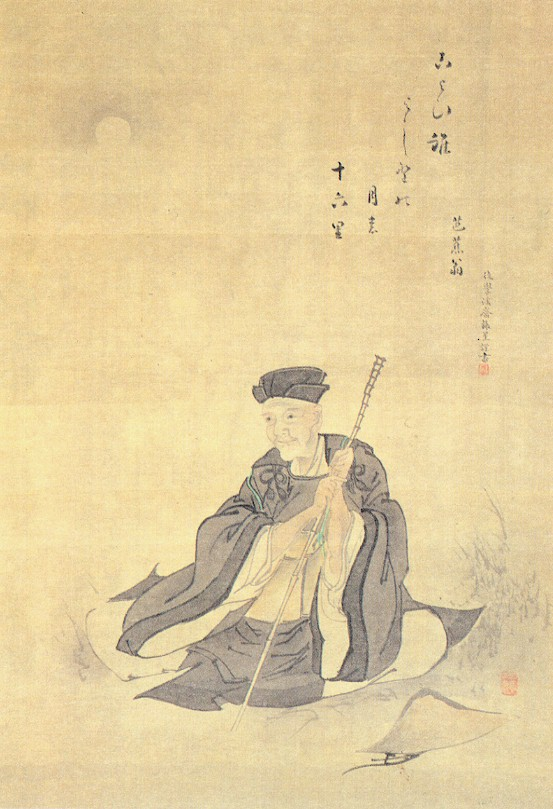
\includegraphics[height=0.9\textheight]{matsuo}\\[1em]
        \large{\FS 松尾芭蕉画像}
    \end{figure}
\end{center}

\newpage

{\FS
    松尾芭蕉(1644—1694)生于伊贺国(今三重县)上野赤坂町下级武士家,原名宗房。幼时陪同藤堂良忠(俳号蝉吟)读书,良忠师事北村季吟,学习贞门俳谐,他对芭蕉有所影响。芭蕉二十三岁时离开家里到京都,向北村季吟学俳谐和古典文学。二十九岁到江户,虽然生活清苦,但努力学俳谐,和当时流行的谈林派俳人交往,也受了影响。三十二岁时,别号桃青,参加西山宗因的俳席。自离开江户城市,过着漂泊的生活,进行艺术的探索,逐渐形成自己的俳风。一六八〇年,三十七岁时,有一批优秀的弟子杉风、卜尺、岚雪、其角等,确立了在俳坛的地位。同年冬,转入隅田川下游东岸的深川六间堀的草庵,以杜甫诗句「门泊东吴万里船」,把草庵称为「泊船堂」,翌年春,在门口种下李下弟子所赠一棵芭蕉,长得茂盛,此庵就叫芭蕉庵,俳号称芭蕉。年底芭蕉庵被别处大火蔓延烧掉,不得不到甲斐国(山梨县)的谷村暂住。一六八三年五月回江户,从此有意过着旅游的生活。一六八四年(四十一岁),开始《野曝纪行》的旅行(又名《甲子行吟》),在名古屋完成第一集《冬日》,奠定了芭蕉风格的基础。翌年四月末回到再建的芭蕉庵,一六八七年八月和弟子曾良、宗波赴常陆国鹿岛旅行写《鹿岛纪行》。十月下旬从江户出发开始《书箱小文》旅行。(《书箱小文》未定稿,后来于一六九一年夏才执笔整理。)归途和弟子越人到信浓国更科,写《更科纪行》。一六八九年三月末带着弟子曾良巡游奥羽北陆,经日光、白河、松岛、平泉、尾花泽、出羽三山、酒田、象潟、出云崎、金泽、福井、敦贺等地,八月下旬至九月初四在大垣停留。全程约二千四百公里,历时六个多月。五年后一六九四年完成《奥州小道》有名的旅行记。他在旅途中,思考诗艺理念问题。一六九〇年,四十七岁,因这次辛苦的旅行,身体不好,移住国分山的幻住庵,出庵前完成《幻住庵记》初稿。一六九一年正月归回故乡伊贺。四五月之间,住在嵯峨落柿舍,留下《嵯峨日记》。九月底离开京都,十月中归回江户,这时已到蕉风的成熟期。芭蕉一生所写的俳谐集有《冬日》、《旷野》、《猿蓑》、《炭包》、《续猿蓑》等七部,这些都是和弟子们一起作的。一六九四年五月又从江户往西旅行,经过奈良,九月末在途中得痢疾,病情恶化,十月八日更深时,给门人支考留下「旅中正卧病,梦绕荒野行」的名句。十月十二日午后在大阪逝世,享年五十一岁。按他的遗嘱,遗体运去葬在膳所的义仲寺内。

    芭蕉经贞门\footnotemark[1]、谈林\footnotemark[2] 两派的俳风,逐步形成自己俳谐的蕉风。到了谈林衰落的后期,他以为作为诗艺的俳谐,当是真诚的,并从传统的继承与发展中,探索新的境界,思考「不易·流行」的艺术观。据研究,所谓「不易」,说的是经越年代还能感人,「流行」说的是随着时代开拓新意境。他认为真诚是俳谐的要素,所谓「不易」与「流行」的作品也是属于同一来源。他要求细致深入地描写对象,钻研美的理念。日本的俳论,一般都称赞他的清寂的代表作「古池塘呀,青蛙跳入响水声」,以一瞬间的小动作的水声,波动了大静的周围,表示作者幽思微情的境界。但是他也写出「坟墓也震动,我的哭声似秋风」那种激情的句子。芭蕉长期旅行接触大自然,写了许多美妙的风光,但也写了一些社会生活,多写自己,也写别人。如「听得猿声悲,秋风又传弃儿啼,谁个最惨凄?」「一年又一年,叫猴戴假面」表现了一定深度的社会性。他常以动物比喻自己,如「离群病雁,落足旅途夜里寒」、「蝴蝶为白罂粟花,撕下翅膀做纪念」等等。

    芭蕉对中国诗文很有素养,他喜爱庄子哲学反俗精神,崇尚杜甫、李白的高逸诗境,这在他的文集句集中反映出来。他把他的处境和心情,写得纯净,富有感人的艺术力。从总体看,他写悲却染有喜色,写喜却含着悲调,晚年要求雅俗浑然融合,创发新意境。他认为平易自然,才是诗艺的妙境。我觉得他晚年许多吟咏秋天情景的作品,饶有这种韵味。

    生活是艺术的源泉,没有旅行,他也就难以写出游记的名作,在游记中闪烁着珠玉般的俳句。他多年漂泊各地,离开城市社会,接触山野人民生活,把深所体会的自然美,升华为艺术美,同时抒写了自己真诚的心灵,创造了独特的艺术风格,也可以说,芭蕉把他的生活沉浸在艺术之中。他的作品,在日本文学史上占有地位,树立了自己的丰碑。他的俳风影响日本俳坛。芭蕉的句碑遍布日本各地,共达三百余座,人们把他尊为「俳圣」。

    \footnotetext[1]{\FS 贞门,松永贞德(1571—1653)拥有一批门徒,倡议不避俗语,但防止过于不雅之词,要求富有生活趣味的诙谐。}

    \footnotetext[2]{\FS 谈林派,以西山宗因(1605—1682)为中心,提倡新风气,倾向市民性,他们的作品的情调较为自由。}
}

\newpage

\section{\FK 新年}

\setcounter{haikucounter}{0}

\begin{haiku}
    {\FH うたがふな、\ruby[g]{潮}{うしお}の花も、浦の春。}

    {\FK 莫疑问,潮头花,亦是滨海春。}
\end{haiku}

\begin{haiku}
    {\FH 元日や、思えばさびし、秋の暮。}

    {\FK 岁旦}

    {\FK 正是年初一,想起暮秋寂寞日。}
\end{haiku}

\begin{haiku}
    {\FH 年々や、猿に着せたる、猿の面。}

    {\FK 一年又一年,叫猴戴假面。}

    {\FT 注:耍猴的,带猴子在肩膀上,挨家逐户打鼓叫猴子跳舞,以求得一点小钱。它和《燕京岁时记》记载的一样,都在新年。此句也有以猴子比喻人的意思。}
\end{haiku}

\begin{haiku}
    {\FH 大津絵の、\ruby[g]{筆}{ふで}のはじめは、何\ruby[g]{仏}{ぼとけ}。}

    {\FK 大津绘,年初落笔是何佛?}

    {\FT 注:大津绘是民间通俗画,元禄年代之前,以佛画居多。岩佐又兵卫擅长佛画,这是作者在人家看到贴着大津绘的即兴句。}
\end{haiku}

\section{\FK 春}

\setcounter{haikucounter}{0}

\begin{haiku}
    {\FH 行く春に、和歌の浦にて、追ひ付きたり。}

    {\FK 和歌浦}

    {\FK 春将归去,追它到和歌浦。}

    {\FT 注:和歌浦在和歌山市南的湾岸一带。}
\end{haiku}

\begin{haiku}
    {\FH 行く春や、鳥啼き魚の、目は泪。}

    {\FK 春将归,鸟啼鱼落泪。}

    {\FT 注:汉诗词常写鱼的自得其乐,宋吴文英《高阳台》却道:「飞红若到西湖底,搅翠澜,总是愁鱼」,适意新颖。芭蕉的鱼落泪,确是不同凡响的佳句。}
\end{haiku}

\begin{haiku}
    {\FH 行く春を、\ruby[g]{近江}{おうみ}の人と、\ruby[g]{惜}{お}しみける。}

    {\FK 望湖水惜春}

    {\FK 我与近江人,同惜春归去。}

    {\FT 注:近江,今滋贺县境内,琵琶湖在这地区。}
\end{haiku}

\begin{haiku}
    {\FH 春なれや、名もなき山の、\ruby[g]{薄}{うす}霞。\footnote{\FT 也有本作《朝霞》。}}

    {\FK 往奈良路上}

    {\FK 春日已来矣,此山何名未得知,薄霭透明媚。}
\end{haiku}

\begin{haiku}
    {\FH 辛崎の、松は花より、\ruby[g]{朧}{おぼろ}にて。}

    {\FK 湖水眺望}

    {\FK 唐崎松比花朦胧。}

    {\FT 注:唐崎,又写作辛崎,在滋贺县大津市琵琶湖的西南岸。在春夜的湖畔,眺望唐崎的松树,为月光映照,浮泛墨绘的景色,看来比那边的樱花更饶朦胧美。}
\end{haiku}

\begin{haiku}
    {\FH 春\ruby[g]{雨}{さめ}や、\ruby[g]{蓬}{よもぎ}をのばす、\ruby[g]{艸}{くさ}の道。}

    {\FK 春雨霏霏芳草径,飞蓬正茂盛。}

    {\FT 注:这句描写春雨,芥川龙之介很赏识它的原句。}
\end{haiku}

\begin{haiku}
    {\FH 春雨や、\ruby[g]{蜂}{はち}の\ruby[g]{巣}{す}つたふ、屋根の\ruby[g]{漏}{も}り。}

    {\FK 屋顶漏春雨,顺着蜂巢点点滴。}

    {\FT 注:屋顶是稻草铺的,芭蕉庵的春雨漏滴声,如在读者心中响着。}
\end{haiku}

\begin{haiku}
    {\FH 水取りや、\ruby[g]{氷}{こおり}の僧の、\ruby[g]{沓}{くつ}の音。}

    {\FK 闲居二月堂}

    {\FK 汲水去,寒僧鞋底声。}

    {\FT 注:奈良东大寺二月堂,二月间有深夜僧众到堂旁若狭井汲水的仪式。僧人穿白衣,举松明,景象十分严肃。}
\end{haiku}

\begin{haiku}
    {\FH 猫の恋、やむとき\ruby[g]{閨}{ねや}の、朧月。}

    {\FK 猫儿叫春停歇时,闺中望见朦胧月。}

    {\FT 注:「猫恋」是俳谐最初季语化的素材。贞门、谈林两派较多吟咏。}
\end{haiku}

\begin{haiku}
    {\FH 鶯や、柳のうしろ、\ruby[g]{薮}{やぶ}の前。}

    {\FK 黄鹂声声啭,听来刚在翠柳后,又在竹林前。}
\end{haiku}

\begin{haiku}
    {\FH 原中や、ものにもつかず、啼く\ruby[g]{雲雀}{ひばり}。}

    {\FK 云雀原野鸣,自由自在一心轻。}
\end{haiku}

\begin{haiku}
    {\FH 雲雀より、空にやすらふ、\ruby[g]{峠}{とうげ}かな。}

    {\FK 脐峠}

    {\FK 小憩于参天峰顶,云雀在下飞鸣。}

    {\FT 注:脐峠今为细峠(奈良县吉野郡吉野町)位于樱井到吉野途中。峠是山巅之意。}
\end{haiku}

\begin{haiku}
    {\FH \ruby[g]{盃}{さかずき}に、\ruby[g]{泥}{どろ}な\ruby[g]{落}{おと}しそ、\ruby[g]{群}{むら}燕。}

    {\FK 楠边}

    {\FK 群燕低飞,碎泥落酒杯。}

    {\FT 注:楠边为朝熊山西麓村落。}
\end{haiku}

\begin{haiku}
    {\FH 古池や、\ruby[g]{蛙}{かわず}飛びこむ、水の音}

    {\FK 古池塘呀,青蛙跳入水声响}

    {\FT 注:这是芭蕉的名作,表示深得清寂幽玄的意境。}
\end{haiku}

\begin{haiku}
    {\FH 蝶よ蝶よ、\ruby[g]{唐土}{もろこし}の、俳諧\ruby[g]{問}{と}はん。}

    {\FK 拜庄周尊像}

    {\FK 蝴蝶哟,蝴蝶,请问何为唐土俳谐。}

    {\FT 注:取庄周梦蝴蝶典故,俳谐含有寓言的意思。}
\end{haiku}

\begin{haiku}
    {\FH 君や蝶、我や\ruby[g]{荘子}{さうじ}が、夢心。}

    {\FK 你哟蝴蝶,我哟庄子,梦之心。}

    {\FT 注:据一六九〇年四月十日书简,芭蕉与怒谁谈论自然之道,十分默契,写此赠句。怒谁和芭蕉都是《庄子》的热心读者。}
\end{haiku}

\begin{haiku}
    {\FH 物好きや、匂はぬ草に、とまる蝶。}

    {\FK 无香杂草里,好奇蝴蝶不离去。}

    {\FT 注:这是作者背离世俗的自喻句。}
\end{haiku}

\begin{haiku}
    {\FH 梅白し、昨日や鶴を、\ruby[g]{盗}{ぬす}まれし。}

    {\FK 梅林}

    {\FK 白梅开正好,白鹤昨天可被盗?}

    {\FT 注:梅林乃京都富豪谈林派俳人三井秋风的别墅。梅鹤风雅,出自林和靖的典故。只见梅不见鹤,以为是被盗了,真煞风景。}
\end{haiku}

\begin{haiku}
    {\FH 忘るなよ、薮の中なる、梅の花。}

    {\FK 莫忘记,梅开在草丛里。}

    {\FT 注:这是赠别句,在草丛里的梅花,喻芭蕉自己。}
\end{haiku}

\begin{haiku}
    {\FH 里の子よ、梅折り残せ、牛の\ruby[g]{鞭}{むち}。}

    {\FK 梅枝作牛鞭,村童哟,请莫折尽。}

    {\FT 注:写村野的情趣。唐朝李群玉咏梅句有「已被儿童苦攀折,更遭风雨损馨香」的诗句。}
\end{haiku}

\begin{haiku}
    {\FH 水鳥の、はしに付たる梅白し。}

    {\FK 水鸟嘴,沾有梅瓣白。}

    {\FT 注:郭沫若以为此作比白居易《春至》诗句「白片落梅浮涧水」更形象化。}
\end{haiku}

\begin{haiku}
    {\FH \ruby[g]{暖簾}{のうれん}の、奥ものふかし、北の梅。}

    {\FK 一有之妻}

    {\FK 暖帘之内,可爱北堂梅。}

    {\FT 注:北堂梅花指一有之妻女俳人斯波园女。园女乃伊势山田秦师贞之女,嫁与同地医师斯波一有为妻,是蕉风门人。}
\end{haiku}

\begin{haiku}
    {\FH 人も見ぬ、春や鏡の、裏の梅。}

    {\FK 无人探春来,镜里梅自开。}

    {\FT 注:镜是古时铜镜。背面铸有梅花,用返照的句法,芭蕉以此自喻。}
\end{haiku}

\begin{haiku}
    {\FH \ruby[g]{数}{かぞ}へ来ぬ、屋敷屋敷の、梅柳。}

    {\FK 缓步}

    {\FK 一路数着来,府邸、府邸之梅柳。}
\end{haiku}

\begin{haiku}
    {\FH 梅が\ruby[g]{香}{か}に、のつと日の出る、山\ruby[g]{路}{じ}哉。}

    {\FK 梅花山路飘香,朝阳猛然出现。}
\end{haiku}

\begin{haiku}
    {\FH 雪\ruby[g]{間}{ま}より、薄紫の、芽\ruby[g]{独活}{うど}哉。}

    {\FK 白雪下,独活呀,冒出浅紫芽。}

    {\FT 注:独活即土当归。此句写白紫对照,新生命的出现。}
\end{haiku}

\begin{haiku}
    {\FH 咲き\ruby[g]{乱}{みだ}す、桃の中より、初櫻。}

    {\FK 桃花丛中见早樱。}
\end{haiku}

\begin{haiku}
    {\FH うち山や、\ruby[g]{外様}{とざま}しらずの、花\ruby[g]{盛}{ざか}り。}

    {\FK 内山花多娇,外人哪知晓。}
\end{haiku}

\begin{haiku}
    {\FH \ruby[g]{鸛}{こふ}の巣に、嵐の\ruby[g]{外}{ほか}の、櫻哉。}

    {\FK 山家}

    {\FK 鹳巢高,山风外樱花闹。}

    {\FT 注:鹳形似鹤,巢筑在高树上。似拟山家主人的口气,讲环境的优越。}
\end{haiku}

\begin{haiku}
    {\FH 木のもとに、\ruby[g]{汁}{しる}も\ruby[g]{膾}{なます}も、桜かな。}

    {\FK 赏花}

    {\FK 树下鱼肉丝、菜汤上,飘落樱花瓣。}

    {\FT 注:记与伊贺人们一起赏樱。历来写樱花很多,这里有鱼肉丝、菜汤的生活气息,显示出平民性。}
\end{haiku}

\begin{haiku}
    {\FH \ruby[g]{阿}{お}蘭\ruby[g]{陀}{だ}も、花に来にけり、馬に\ruby[g]{鞍}{くら}。}

    {\FK 荷兰人,马挂鞍来赏樱。}

    {\FT 注:荷兰驻长崎商馆馆长,每年到江户赏樱,并拜谒江户将军。}
\end{haiku}

\begin{haiku}
    {\FH 京は九万、九千くんじゅの、花見哉。}

    {\FK 京都看花天,群集九万九千。}
\end{haiku}

\begin{haiku}
    {\FH 花にうき世、我が酒白く、飯黒し。}

    {\FK 忧方知酒圣,贫始觉钱神}

    {\FK 对花忧人间,我酒浊饭淡。}

    {\FT 注:题是白居易《江南谪居十韵》的诗句。}
\end{haiku}

\begin{haiku}
    {\FH 花咲きて、七日鶴見る、\ruby[g]{麓}{ふもと}哉。}

    {\FK 三月廿日即兴}

    {\FK 山麓花盛开,七天鹤常在。}

    {\FT 注:比睿山麓,花开春色美好,白鹤在那周内也飞来玩赏。}
\end{haiku}

\begin{haiku}
    {\FH 花の雲、\ruby[g]{鐘}{かね}は上野か、浅草か。}

    {\FK 草庵}

    {\FK 花云缥缈,钟声来自上野,还是浅草?}

    {\FT 注:花云指樱花如轻云。该庵在江户郊外,可以听到上野或浅草的钟声。}
\end{haiku}

\begin{haiku}
    {\FH 何の木の、花とはしらず、匂かな。}

    {\FK 伊势山田}

    {\FK 不知何树花开,香气扑鼻来。}
\end{haiku}

\begin{haiku}
    {\FH しばらくは、花の上なる、月夜かな。}

    {\FK 春月夜,暂且逗留花蕊上。}

    {\FT 注:花即樱花,这是描绘月和花的静美。}
\end{haiku}

\begin{haiku}
    {\FH 四方より、花吹き入れて、鳰の波。}

    {\FK 洒落堂记}

    {\FK 四方飘下花雪来,尽归䴙䴘海。}

    {\FT 注:四方即琵琶湖四周,指唐崎、比睿、比良、三上诸山。䴙䴘是一种水鸟,俗称水葫芦,琵琶湖又称䴙䴘海。这是写从洒落堂(主人是滨田珍夕医师)眺望琵琶湖的春日风光。}
\end{haiku}

\begin{haiku}
    {\FH 年々や、桜を\ruby[g]{肥}{こ}やす、花の\ruby[g]{塵}{ちり}。}

    {\FK 年年樱瓣飞,花屑化作肥。}

    {\FT 注:这是落红化作春泥的意思。}
\end{haiku}

\begin{haiku}
    {\FH わが\ruby[g]{衣}{きぬ}に、\ruby[g]{伏見}{ふし}の桃の、雫せよ。}

    {\FK 伏见西岸寺遇任口上人}

    {\FK 请将伏见桃花露,滴落我衣襟。}

    {\FT 注:伏见为京都市南区一部,一五九四年丰臣秀吉在桃山筑伏见城,该城为桃名所。任口上人在西岸寺任职,芭蕉尊重这位老前辈。}
\end{haiku}

\begin{haiku}
    {\FH \ruby[g]{草臥}{くたぶ}れて、\ruby[g]{宿}{やど}かる頃や、藤の花。}

    {\FK 太和行脚时}

    {\FK 投宿已疲乏,忽又见藤花。}

    {\FT 注:藤花在暮霭中有凋谢状,看了更感困倦。}
\end{haiku}

\begin{haiku}
    {\FH ほろほろと、山吹ちるか、滝の音。}

    {\FK 西河}

    {\FK 棣棠落花簌簌,可是激湍漉漉?}

    {\FT 注:写和歌山县吉野川岸畔的景致。原文有双声的句法。}
\end{haiku}

\begin{haiku}
    {\FH 菜\ruby[g]{畠}{ばたけ}に、花見顔なる、\ruby[g]{雀}{すずめ}哉。}

    {\FK 行吟}

    {\FK 菜花开满园,麻雀赏花颜。}
\end{haiku}

\begin{haiku}
    {\FH \ruby[g]{躑躅}{つつじ}生けて、その陰に\ruby[g]{干鱈}{ひだら}、\ruby[g]{割}{さ}く女。}

    {\FK 坐在茶店午休}

    {\FK 桶内插杜鹃,阴凉里,女佣撕裂鳕鱼干。}

    {\FT 注:写客栈女佣撕鳕鱼,准备客饭,可看出俳谐的生活化、通俗化。}
\end{haiku}

\begin{haiku}
    {\FH 山路来て、何やらゆかし、菫草。}

    {\FK 越过山道,去大津路上}

    {\FK 山路费攀登,竟有可爱紫地丁。}
\end{haiku}

\begin{haiku}
    {\FH よく見れば、\ruby[g]{薺}{なずな}花咲く、\ruby[g]{垣}{かき}根かな。}

    {\FK 细看墙根下,竟然开荠花。}

    {\FT 注:白居易诗句有「惆怅去年墙下地,今春唯有荠花开」。情景相似。}
\end{haiku}

\begin{haiku}
    {\FH \ruby[g]{衰}{おとろ}ひや、歯に喰ひ\ruby[g]{当}{あ}てし、\ruby[g]{海苔}{のり}の砂。}

    {\FK 啮到紫菜砂,感叹老衰牙。}
\end{haiku}

\section{\FK 夏}

\setcounter{haikucounter}{0}

\begin{haiku}
    {\FH 六月や、峰に雲置く、嵐山。}

    {\FK 嵯峨}

    {\FK 六月岚山云遮峰。}

    {\FT 注:六月炎暑,岚山满山苍翠,夏云遮掩山峰。岚山在京都市西部嵯峨地区,在大堰川右岸,自平安朝以来,为红叶与樱花的名所。}
\end{haiku}

\begin{haiku}
    {\FH 秋近き、心の寄るや、四\ruby[g]{畳}{じょう}半。}

    {\FK 元禄七年六月廿一日于大津木节家}

    {\FK 秋近心相连,四席半。}

    {\FT 注:元禄七年一六九四年,芭蕉与各务支考、广濑惟然聚会于望月木节家,在四席半小房间,设有俳谐席。}
\end{haiku}

\begin{haiku}
    {\FH 五月雨に、鳰の浮巣を、見にゆかん。}

    {\FK 致露沾公}

    {\FK 黄梅雨里,看䴙䴘浮巢去}

    {\FT 注:露沾公乃磐城内藤义英,江户俳坛的后援人。}
\end{haiku}

\begin{haiku}
    {\FH 五月雨に、隠れぬものや、瀬田の橋。}

    {\FK 湖景遮掩梅雨中,濑田桥横。}

    {\FT 注:这像一幅浮世绘名家广重的画。濑田桥为日本三大桥之一。}
\end{haiku}

\begin{haiku}
    {\FH 五月雨の、降り残してや、\ruby[g]{光堂}{ひかりどう}。}

    {\FK 梅雨落剩一光堂。}

    {\FT 注:光堂即金色堂。一一八五年为藤原洁衡所建,作为自己死后的坟墓。据记载佛殿内外,施贴金箔,镂嵌螺钿,极尽庄严豪华之美。此句指几百年来年年落梅雨,于今光堂仍辉煌地存在着。}
\end{haiku}

\begin{haiku}
    {\FH 降る音や、耳も\ruby[g]{酸}{す}うなる、梅の雨。}

    {\FK 梅雨声不断,耳朵也发酸。}

    {\FT 注:酸和梅是相关语。这是芭蕉二十三岁时的吟句。}
\end{haiku}

\begin{haiku}
    {\FH 五月雨を、集めて早し、最上川。}

    {\FK 梅雨收集遍,奔流最上川。}

    {\FT 注:最上川在山形县境内,为日本三大急流之一。}
\end{haiku}

\begin{haiku}
    {\FH 松杉を、ほめてや風の、かをる音。}

    {\FK 在小仓山常寂寺}

    {\FK 赞美松杉,薰风声喧。}

    {\FT 注:小仓山在嵯峨里面,松杉翠绿,薰风南来,好似赞美它们一样。}
\end{haiku}

\begin{haiku}
    {\FH このあたり、目に見ゆるものは、皆涼し。}

    {\FK 十八楼记}

    {\FK 望此方,眼底景物皆清凉。}

    {\FT 注:十八楼乃稻叶山麓加岛鸥步(歧阜俳人)的水楼,可以眺望长良川远近的农村渔村和北部的群山诸景。}
\end{haiku}

\begin{haiku}
    {\FH 涼しさを、絵にうつしけり、\ruby[g]{嵯峨}{さが}の竹。}

    {\FK 野明家}

    {\FK 嵯峨竹,清凉入画图。}

    {\FT 注:野明即奥西善六,居嵯峨,称坂井作大夫。嵯峨在京都市西部,多竹。}
\end{haiku}

\begin{haiku}
    {\FH \ruby[g]{蛸壺}{たこつぼ}や、はかなき夢を、夏の月。}

    {\FK 明石夜泊}

    {\FK 夏月夜,章鱼壶中虚幻梦。}

    {\FT 注:明石在兵库县南部,面临播磨滩,那里有陶壶捕章鱼的办法。这是写章鱼已经被捕了,还在做梦。}
\end{haiku}

\begin{haiku}
    {\FH さざれ蟹、足\ruby[g]{這}{は}ひのぼる、清水哉。}

    {\FK 螃蟹小又细,爬上我双足,泉水多清冽。}
\end{haiku}

\begin{haiku}
    {\FH 馬ぼくぼく、我を絵に見る、夏野かな。}

    {\FK 画赞}

    {\FK 马蹄迟迟夏野行,看我身在画图中。}
\end{haiku}

\begin{haiku}
    {\FH \ruby[g]{笈}{おい}も\ruby[g]{太刀}{たち}も、\ruby[g]{五月}{さつき}に飾れ、紙\ruby[g]{幟}{のぼり}。}

    {\FK 大刀与背箱,可同纸旗装饰五月天。}

    {\FT 注:源义经的大刀、弁庆的背箱。源义经(1159—1189)镰仓初期名将,源义朝第九子,扶助其兄源赖朝,讨伐源义仲,又在坛浦击灭平氏。为其兄赖朝所忌,终于被迫自杀。弁庆(?—1189)僧人,义经的从臣,为义经而战死。纸旗画鲤鱼或钟馗等,在端午节前后挂在空中。}
\end{haiku}

\begin{haiku}
    {\FH おもしろうて、やがて悲しき、\ruby[g]{鵜舟}{うぶね}かな。}

    {\FK 鸬鹚船,兴致舒畅,黯然转神伤。}

    {\FT 注:芭蕉在歧阜长良川即景句。捕取鲇鱼的鸬鹚船,先是点燃熊熊的篝火,顺流而下,篝火渐渐消灭,船在黑暗中归去。作者以「欢乐尽而情深」的心理写出。}
\end{haiku}

\begin{haiku}
    {\FH 涼ぬとて、切りぬけにたり、北の窓。}

    {\FK 请纳凉,北墙凿通个小窗。}

    {\FT 注:郭沫若以为此作与汉诗「暑月贫家何所有,客来惟赠北窗风」相近。}
\end{haiku}

\begin{haiku}
    {\FH 雲の峰、いくつ崩れて、月の山。}

    {\FK 几道云峰解散,新月耀辉东土。}

    {\FT 注:《奥州小道》记月山、羽黑山和汤殿山为出羽三山的高峰,句将月山拆开描写。}
\end{haiku}

\begin{haiku}
    {\FH 命なり、わづかの笠の、下涼み。}

    {\FK 佐夜中山}

    {\FK 命也如是,只有草笠下,稍得些凉意。}

    {\FT 注:佐夜中山,今静冈县小笠、榛原二郡之间险峻的山道。当越此山时,一路不见树荫,炎热焦灼,故发此感慨。}
\end{haiku}

\begin{haiku}
    {\FH 降らずとも、竹\ruby[g]{植}{う}うる日は、\ruby[g]{蓑}{みの}と笠。}

    {\FK 竹}

    {\FK 种竹日,不下雨,也要蓑和笠。}

    {\FT 注:种竹日来自中国「竹醉日」即五月十三日,该日种竹易活。因是梅雨时节,故要蓑和笠。}
\end{haiku}

\begin{haiku}
    {\FH \ruby[g]{鹿}{しか}の\ruby[g]{角}{つの}、まづ\ruby[g]{一節}{ひとふし}の、わかれかな。}

    {\FK 奈良别旧友}

    {\FK 鹿角首节先分枝。}

    {\FT 注:旧友指从伊贺故乡来的猿虽、卓袋诸人。最初的鹿角分枝,表示不得不离的意思。这是酬唱之作。}
\end{haiku}

\begin{haiku}
    {\FH ほととぎす、消え行く方や、島一つ。}

    {\FK 杜鹃飞去已无声,那方只余孤岛景。}

    {\FT 注:据纪行《书箱小文》,从铁拐山向海上瞭望的岛,即淡路岛。该岛在神户西部须磨海岸附近。}
\end{haiku}

\begin{haiku}
    {\FH \ruby[g]{一声}{ひとこえ}の、江に横\ruby[g]{たふ}{とう}や、ほととぎす。}

    {\FK 时鸟声横江水上。}

    {\FT 注:「横江」据说来自《前赤壁赋》的「白露横江,水光接天」和《后赤壁赋》的「适有孤鹤,横江东来」。}
\end{haiku}

\begin{haiku}
    {\FH 鶯や、竹の子薮に、\ruby[g]{老}{おい}を鳴く。}

    {\FK 笋竹丛中莺声老。}

    {\FT 注:芭蕉自老莺,看新生笋竹,便感叹起老来。}
\end{haiku}

\begin{haiku}
    {\FH \ruby[g]{閑}{しずけ}さや、\ruby[g]{岩}{いわ}にしみ入る、蝉の声。}

    {\FK 静寂呀,蝉声入岩石。}

    {\FT 注:此句可与王籍诗「蝉噪林愈静,鸟鸣山更幽」比,作此是因蝉噪、鸟鸣才显得环境更幽静。}
\end{haiku}

\begin{haiku}
    {\FH やがて死ぬ、けしきは見えず、蝉の声。}

    {\FK 无常迅速}

    {\FK 知了在叫,不知死期快到。}

    {\FT 注:有庄子《逍遥游》「蝼蛄不知春秋」句意}
\end{haiku}

\begin{haiku}
    {\FH 草の葉を、落つるより飛ぶ、蛍哉。}

    {\FK 萤火虫,刚落下草丛,就从草丛飞升。}

    {\FT 注:这是抓住两个动作的瞬间,微妙地表示萤火虫的形态。}
\end{haiku}

\begin{haiku}
    {\FH \ruby[g]{蚤虱}{のみしらみ}、馬の\ruby[g]{尿}{ばり}する、枕もと。}

    {\FK 蚤虱横行,枕畔又闻马尿声。}

    {\FT 注:《奥州小道》的旅行,记在尿前山区中寄宿农家,人马同室的情景。}
\end{haiku}

\begin{haiku}
    {\FH 若\ruby[g]{葉}{ば}して、\ruby[g]{御目}{おんめ}の雫、ぬぐはばや。}

    {\FK 新叶滴翠,摘来拂拭尊师泪。}

    {\FT 注:这是到奈良唐招提寺,拜谒盲圣鉴真像之句。}
\end{haiku}

\begin{haiku}
    {\FH あらたふと、青葉若葉の、日の光。}

    {\FK 访日光山}

    {\FK 好辉煌,浓淡绿叶映日光。}

    {\FT 注:一六八九年四月一日,参谒日光东照宫时所作。}
\end{haiku}

\begin{haiku}
    {\FH 須磨\ruby[g]{寺}{でら}や、吹かぬ\ruby[g]{笛}{ふえ}聞く、\ruby[g]{木}{こ}下闇。}

    {\FK 须磨寺,树荫暗处,听此不吹笛。}

    {\FT 注:须磨寺在神户市须磨区,即上野山福祥寺。该寺有名贵文物——平敦盛的青叶笛。源平在一谷会战时,平敦盛腰间挂着心爱的笛子。这是芭蕉的幻想句,想象听到昔日的笛声。}
\end{haiku}

\begin{haiku}
    {\FH \ruby[g]{駿}{する}\ruby[g]{河}{が}路や、花橘も、茶の匂ひ。}

    {\FK 入骏河国}

    {\FK 骏河路上,花桔发茶香。}

    {\FT 注:骏河路,在静冈地区,这条路上,到处白橘花盛开。这里又是制茶的地方,橘花香中也有茶香。}
\end{haiku}

\begin{haiku}
    {\FH \ruby[g]{杜若}{かきつばた}、\ruby[g]{語}{かた}るも旅の、ひとつかな。}

    {\FK 在大阪}

    {\FK 杜若作话题,也是一种旅中趣。}

    {\FT 注:杜若,生在水边,初夏开紫花,又名燕子花。这是旅中与门徒小杉一笑交谈的即兴句。}
\end{haiku}

\begin{haiku}
    {\FH \ruby[g]{菖蒲}{あやめ}草、足に\ruby[g]{結}{むすば}ん、\ruby[g]{草履}{わらじ}の緒。}

    {\FK 菖蒲结做草鞋带,绑在行脚上。}

    {\FT 注:端午节挂菖蒲在檐下避邪,现在绑在脚上,为旅行吉利。}
\end{haiku}

\begin{haiku}
    {\FH 白\ruby[g]{芥子}{げし}に、羽もぐ蝶の、形見かな。}

    {\FK 蝴蝶为白罂粟花,撕下翅膀作纪念。}

    {\FT 注:写他与弟子杜国惜别的强烈感情。蝴蝶比自己,白罂粟比杜国。}
\end{haiku}

\begin{haiku}
    {\FH 撫子に、かかる涙や、\ruby[g]{楠}{くす}の露。}

    {\FK 正成之像\\铁肝石心此人之情}

    {\FK 楠露滴落石竹泪。}

    {\FT 注:写楠木正成(1294—1336)父子在樱井驿诀别悲剧(《太平记》卷一六)的画赞,把石竹当作当时十一岁的正行,把楠木叶滴落的露,作力父亲慈爱的泪,泪滴在树荫下开花的石竹上。}
\end{haiku}

\begin{haiku}
    {\FH 世の人の、見付けぬ花や、\ruby[g]{軒}{のき}の\ruby[g]{栗}{くり}。}

    {\FK 不为世人注意,檐下栗花枝。}
\end{haiku}

\begin{haiku}
    {\FH \ruby[g]{象潟}{きさがた}や、雨に\ruby[g]{西施}{せいし}が、\ruby[g]{合歓}{ねぶ}の花。}

    {\FK 象潟合欢,恰似雨中西施。}

    {\FT 注:象潟今秋田县由利郡象潟汀海滨,雨中合欢花像颦眉泪湿的西施。}
\end{haiku}

\begin{haiku}
    {\FH 朝露や、よごれて涼し、\ruby[g]{瓜}{うり}の泥。}

    {\FK 在去来别墅}

    {\FK 朝露湿瓜泥,黑汙而冷冽。}

    {\FT 注:向井去来乃蕉门十哲之一。芭蕉在夏天早晨步入瓜田地,看到露水和泥土的即景句。}
\end{haiku}

\begin{haiku}
    {\FH 夏来ても、ただひとつ葉の、一葉かな。}

    {\FK 虽是夏天来,石苇依然只一叶。}

    {\FT 注:石苇是生于山野的羊齿类,只长强韧的一片长叶,寒冬不枯萎。这含有孤高之意。}
\end{haiku}

\begin{haiku}
    {\FH 清滝や、波に散り込む、青松葉。}

    {\FK 清泷眺望}

    {\FK 松叶青青,散落清泷波心。\footnote{\FT 此为芭蕉去世前三日在大阪所做。}}

    {\FT 注:清泷即清泷川,在京都郊外梅尾高山寺前流入大堰川,流狭水清。落在波心的,是被薰风刮下的青松叶,并非落叶。}
\end{haiku}

\begin{haiku}
    {\FH 夏草や、\ruby[g]{兵}{つわもの}どもが、夢の跡。}

    {\FK 在奥州高馆}

    {\FK 长夏草木深,武士当年梦痕。}

    {\FT 注:高馆是为源义经建筑的城楼。武士指为源义经而战的家臣。}
\end{haiku}

\begin{haiku}
    {\FH 夏草に、富貴を飾れ、蛇の\ruby[g]{衣}{きぬ}。}

    {\FK 繁茂夏草里,装点富贵蛇衣。}

    {\FT 注:这是在幻住庵的吟作。蛇衣外观华丽,故云能装点富贵。}
\end{haiku}

\section{\FK 秋}

\setcounter{haikucounter}{0}

\begin{haiku}
    {\FH 初秋や、海も青田も、一みどり。}

    {\FK 鸣海眺望}

    {\FK 初秋时节,碧海青田一色。}

    {\FT 注:鸣海,今名古屋市绿巴鸣海町,附近海岸称为鸣海湾。}
\end{haiku}

\begin{haiku}
    {\FH 牛部屋に、\ruby[g]{蚊}{か}の声暗き、残暑哉。}

    {\FK 牛棚残暑蚊声暗。}

    {\FT 注:牛棚暗,听蚊声也暗。这与「鸭声白」同是「通感」句法。初稿是「秋声起,牛棚蚊声低。」}
\end{haiku}

\begin{haiku}
    {\FH 野ざらしを、心に風の、しむ身かな。}

    {\FK 此身或将曝荒原,风吹入骨寒。}

    {\FT 注:一六八四年秋,从江户出发长途旅行,此是《野曝纪行》的首句。}
\end{haiku}

\begin{haiku}
    {\FH 枯枝に、\ruby[g]{烏}{からす}のとまりたるや、秋の暮。}

    {\FK 寒鸦宿枯枝,深秋日暮时。}

    {\FT 注:拟汉诗句题材,有古典情趣。使人忆起马致远《天净沙》「枯藤老树昏鸦」句。}
\end{haiku}

\begin{haiku}
    {\FH この道を、行く人なしに、秋の暮。}

    {\FK 所思}

    {\FK 秋日黄昏,此路无行人。}

    {\FT 注:与寒山「古道无人行,秋风动禾黍」句,不无关联。}
\end{haiku}

\begin{haiku}
    {\FH 秋の夜を、打ち崩したる、\ruby[g]{咄}{はなし}かな。}

    {\FK 菊月二十一日潮江车庸家}

    {\FK 谈笑风生,打破秋夜静。}

    {\FT 注:菊月是旧历九月,车庸是蕉门弟子,大阪富裕的市民。}
\end{haiku}

\begin{haiku}
    {\FH \ruby[g]{髭}{ひげ}風を、吹いて\ruby[g]{暮秋}{ぼしゅう}嘆ずるは、誰が子ぞ。}

    {\FK 忆老杜}

    {\FK 西风拂须时,感叹深秋者谁子?}

    {\FT 注:原文老杜即杜甫。此作与杜甫《白帝城最高楼》「杖藜叹世者谁子」句法相似。}
\end{haiku}

\begin{haiku}
    {\FH 松風や、軒をめぐって、秋暮れぬ。}

    {\FK 惜秋}

    {\FK 松风绕屋吹,秋将归。}
\end{haiku}

\begin{haiku}
    {\FH \ruby[g]{蛤}{はまぐり}の、ふたみにわかれ、行秋ぞ。}

    {\FK 蚌壳蚌肉苦分离,秋将归去时。}

    {\FT 注:蚌是二见浦的名产。二见发音与壳身同,有双关意,写出在伊势二见浦辞别亲人的苦痛。这是《奥州小道》里最后的俳句。}
\end{haiku}

\begin{haiku}
    {\FH 行く秋の、なほ頼もしや、青蜜柑。}

    {\FK 晚秋景寂然,赖有青桔装点。
    }

    {\FT 注:晚秋景象萧瑟,幸有青桔金黄色缀景。}
\end{haiku}

\begin{haiku}
    {\FH 荒海や、佐渡によこたふ、天河。}

    {\FK 大海波翻,银河横挂佐渡天。}

    {\FT 注:佐渡,地名,新潟县西的一个岛,宗教家日莲上人,文艺家藤原为兼、世阿弥等曾被流放此地。句意与杜甫的「渭水银河清,横天流不息」不无联系。}
\end{haiku}

\begin{haiku}
    {\FH \ruby[g]{稲妻}{いなづま}を、手にとる闇の、\ruby[g]{紙燭}{しそく}哉。}

    {\FK 寄李下}

    {\FK 闪电在手,黑暗中当烛光。}

    {\FT 注:李下为芭蕉门人,正在探索俳谐新境界,芭蕉以此句赞他。}
\end{haiku}

\begin{haiku}
    {\FH 稲妻や、闇の方行く、五位の声。}

    {\FK 闪电明,暗处苍鳽声。}

    {\FT 注:苍鳽(鹭之一种)夜间一边飞一边叫,声难听,翅膀发光。这是与闪电照应,也带怪异味。\footnote{\FT「五位」,指五位鹭,中文名夜鹭。}}
\end{haiku}

\begin{haiku}
    {\FH 吹き飛ばす、石は浅間の、\ruby[g]{野分}{のわき}かな。}

    {\FK 浅间山大风起,飞沙又走石。}

    {\FT 注:浅间山是在长野、群马两县之间的活火山。}
\end{haiku}

\begin{haiku}
    {\FH 猿を聞人、捨子に秋の、風いかに。}

    {\FK 听得猿声悲,秋风又传弃儿啼,谁个最惨凄?}

    {\FT 注:《野曝纪行》旅中经富士川畔时,听到三岁弃儿悲惨的哭声,便联想唐诗的猿啼,因而作此对比的提问。}
\end{haiku}

\begin{haiku}
    {\FH \ruby[g]{義朝}{よしとも}の、心に似たり、秋の風。}

    {\FK 秋风萧森,宛似义朝心。}

    {\FT 注:源义朝,平安末期的武将。后战败落魄美浓路,在尾张为家臣所杀。}
\end{haiku}

\begin{haiku}
    {\FH 秋風や、薮も\ruby[g]{畠}{はたけ}も、\ruby[g]{不破}{ふわ}の関。}

    {\FK 不破关}

    {\FK 不破关口秋风,吹过田原草丛。}

    {\FT 注:不破关乃古歌吟咏的名所,它在歧阜县不破郡关原町。奈良时代与铃鹿、爱发,称为三关。平安时代被废,成为古关。写它颓残的遗迹。}
\end{haiku}

\begin{haiku}
    {\FH \ruby[g]{塚}{つか}も動け、わが泣く声は、秋の風。}

    {\FK 坟墓也震动,我的哭声似秋风。}

    {\FT 注:芭蕉哭的是门下小杉一笑,在芭蕉到金泽前一年死去,终年三十六岁。句写出强烈的感情。}
\end{haiku}

\begin{haiku}
    {\FH 唐\ruby[g]{破}{は}\ruby[g]{風}{ふ}の、入日や薄き、夕涼み。}

    {\FK 途中吟}

    {\FK 彤彤夕日虽无情,凉爽又秋风。}

    {\FT 注:入金泽途中吟句。说炎夏必将过去,秋天随着到来。}
\end{haiku}

\begin{haiku}
    {\FH 石山の、石より白し、秋の風。}

    {\FK 诣那谷观音}

    {\FK 比起石山石,秋风色更白。}

    {\FT 注:石山指小松市那谷町那谷寺的山岩,比近江石山寺的石更白,对萧瑟的秋风,也有白色感觉的联想。注释者引用中国古有「春青、夏赤、秋白、冬黑」的说法。}
\end{haiku}

\begin{haiku}
    {\FH \ruby[g]{名月}{めいげつ}や、池をめぐりて、夜もすがら。}

    {\FK 秋月明,一夜绕池行。}

    {\FT 注:月是仲秋的月,池是芭蕉庵旁的池。}
\end{haiku}

\begin{haiku}
    {\FH 月見する、座にうつくしき、顔もなし。}

    {\FK 古寺玩月}

    {\FK 明月照座间,不见美容颜。}

    {\FT 注:谣曲《三井寺》有住僧与寺童(留发穿好看衣服的美少年)赏月的场面。此句写从幻想到现实的景象。}
\end{haiku}

\begin{haiku}
    {\FH 芭蕉葉を、\ruby[g]{柱}{はしら}に懸けん、\ruby[g]{庵}{いお}の月。}

    {\FK 移植芭蕉词}

    {\FK 新庵明月,照见柱悬芭蕉叶。}

    {\FT 注:一六九二年五月,门人在深川旧居附近新建芭蕉庵。八月移植芭蕉到新居院子,在柱子悬挂蕉叶是为赏月助兴。}
\end{haiku}

\begin{haiku}
    {\FH 名月や、門にさしくる、潮がしら。}

    {\FK 深川}

    {\FK 月明如昼,门前涌入潮头。}

    {\FT 注:芭蕉庵靠近隅田川的河口,满潮时,月光映照潮头。虽写实景,也感到一种生命力。}
\end{haiku}

\begin{haiku}
    {\FH 三井寺の、\ruby[g]{門}{もん}\ruby[g]{敲}{たた}かばや、今日の月。}

    {\FK 今夜三井寺,月亮来敲门。}

    {\FT 注:此句将贾岛「僧敲月下门」改作,芭蕉等人泛舟赏月,兴余访三井寺的千那、尚白。}
\end{haiku}

\begin{haiku}
    {\FH 月見せよ、玉江の\ruby[g]{芦}{あし}を、\ruby[g]{刈}{か}らぬ先。}

    {\FK 玉江}

    {\FK 赏月哟,玉江芦苇割掉前。}

    {\FT 注:玉江芦苇在古歌中有名。玉江,今福井市足羽郡麻生津的江川。割苇前可欣赏月色如水,苇穗摇曳的景色。}
\end{haiku}

\begin{haiku}
    {\FH \ruby[g]{米}{よね}くるる、友を今宵の、月の客。}

    {\FK 十五夜}

    {\FK 今宵且将赠米人,作为赏月嘉宾。}

    {\FT 注:一六九一年八月十五日在草庵集合门人赏月,其中膳所的门人正秀曾给芭蕉送过二斗米。}
\end{haiku}

\begin{haiku}
    {\FH 月ぞしるべ、こなたへ入せ、旅の宿。}

    {\FK 月亮是老相识,请来这儿住宿。}

    {\FT 注:谣曲《鞍马天狗》有「花儿当向导,请到这儿来!」句,一六六四年芭蕉廿岁时,据此改作。}
\end{haiku}

\begin{haiku}
    {\FH 馬に寝て、\ruby[g]{残夢}{ざんむ}月遠し、茶のけぶり。}

    {\FK 迷蒙马背眠,月随残梦天边远,淡淡起茶烟。}

    {\FT 注:写天未明出发的情景。有杜牧《早行》残梦的意境。又想起苏轼的「马上续残梦,不知朝日升」诗句。}
\end{haiku}

\begin{haiku}
    {\FH 月はやし、\ruby[g]{梢}{こずえ}は雨を、持ちながら。}

    {\FK 月儿移行急,枝梢掩留雨滴。}

    {\FT 注:雨夜还有月亮,乌云移动快,显得月亮也步伐匆忙。}
\end{haiku}

\begin{haiku}
    {\FH あの中に、\ruby[g]{蒔}{まき}絵書きたし、宿の月。}

    {\FK 茅店月,欲往自身绘泥金。}

    {\FT 注:旅宿山中,看月亮的美,想象在月上绘泥金画。}
\end{haiku}

\begin{haiku}
    {\FH \ruby[g]{俤}{おもかげ}や、\ruby[g]{姥}{おば}ひとり泣く、月の友。}

    {\FK 弃老山}

    {\FK 老妪独自泣,愁容赏月友。}

    {\FT 注:弃老山在长野县更植市八幡西部。《太和物语》、《今昔物语》、《谣曲》均有此传说,说住在更科的一个汉子,养活老母,受媳妇的挑唆,竟在中秋明月之夜,将老母抛弃在深山里之后,受良心的谴责,翌晨又带她回家。人们在弃老山赏月,说曾出现老妇的姿影。}
\end{haiku}

\begin{haiku}
    {\FH 月影や、四門四宗も、ただ一つ。}

    {\FK 善光寺}

    {\FK 明月只一轮,普照四宗四门。}

    {\FT 注:普光寺乃长野市元善町的名刹。四宗指显、密、禅、戒,又说是天治、真言、禅、律。四门指发心、修行、菩提、涅槃。此外还有别的解释。}
\end{haiku}

\begin{haiku}
    {\FH 義\ruby[g]{仲}{なか}の、寝覚めの山か、月悲し。}

    {\FK 燧城}

    {\FK 义仲夜半醒,燧山月凄清。}

    {\FT 注:燧城是木曾义仲军为平维盛攻陷的古战场(《平家物语》卷七),在汤尾岭的对侧燧山。这是写败将义仲的心情,乃吊古之作。}
\end{haiku}

\begin{haiku}
    {\FH 月いづく、鐘は沈める、海の\ruby[g]{底}{そこ}。}

    {\FK 吊钟沉海底,明月何处去?}

    {\FT 注:中秋夜在敦贺(今福井县敦贺市),未见明月,想是传说所云,月亮寻找沉钟去了。}
\end{haiku}

\begin{haiku}
    {\FH 川\ruby[g]{上}{かみ}と、この川\ruby[g]{下}{しも}や、月の友。}

    {\FK 泛舟于深川尾五棵松处}

    {\FK 此川上下游,同是月之友。}

    {\FT 注:句中的川,小名叫木川,上游阿武地区有俳人素堂住所,下游六间堀为芭蕉庵,此是芭蕉下游处泛舟赏月的吟咏,也想到上游有人在赏月。}
\end{haiku}

\begin{haiku}
    {\FH 汐越や、鶴\ruby[g]{脛}{はぎ}ぬれて、海涼し。}

    {\FK 秋月明,鹤胫亭亭,远立海滩滨。}
\end{haiku}

\begin{haiku}
    {\FH 夜る\ruby[g]{竊}{ひそか}に、虫は月下の、栗を\ruby[g]{穿}{うが}つ。}

    {\FK 果虫做夜偷,钻进月下栗里头。}

    {\FT 注:《和汉朗咏集》傅温有「夜雨偷穿石上苔」句,芭蕉也用偷字。}
\end{haiku}

\begin{haiku}
    {\FH 西行の、草鞋もかかれ、松の露。}

    {\FK 画赞}

    {\FK 西行上人,草鞋亦沾松露。}

    {\FT 注:西行(1181—1190)是身穿袈裟,云游四方的歌人,著有《山家集》。}
\end{haiku}

\begin{haiku}
    {\FH 霧しぐれ、富士を見ぬ日ぞ、おもしろき。}

    {\FK 过箱根关所时遇雨山云迷漫}

    {\FK 濛濛烟雨,不见富士山姿,另有情趣。}
\end{haiku}

\begin{haiku}
    {\FH 手にとらば、消えん涙ぞ熱き、秋の霜。}

    {\FK 手上捧秋霜,因落热泪而消溶。}

    {\FT 注:一六八四年秋,芭蕉回故乡,拜见亡母的遗发,不禁热泪滚落。他把白发比做秋霜,故会因热泪而溶化。写出对亡母的敬爱深情。}
\end{haiku}

\begin{haiku}
    {\FH \ruby[g]{合歓}{ねむ}の木の、葉越しも\ruby[g]{厭}{いと}へ、星の影。}

    {\FK 七夕}

    {\FK 星之光,厌照合欢树叶间。}

    {\FT 注:七夕牛郎织女双星难得相逢,无心俯视合欢花树荫。}
\end{haiku}

\begin{haiku}
    {\FH 七夕の、\ruby[g]{逢}{あ}はぬ心や、雨中天。}

    {\FK 七夕雨中天,心恨不得重相见。}

    {\FT 注:心指牛郎和织女的心。}
\end{haiku}

\begin{haiku}
    {\FH 家はみな、\ruby[g]{杖}{つえ}に\ruby[g]{白髪}{しらが}の、墓参り。}

    {\FK 亲人皆白发,扶杖扫坟去。}

    {\FT 注:一六九四年,得兄(松尾半左卫门)信,还回故乡,参加盂兰盆会,与亲戚老辈一起扫坟去。}
\end{haiku}

\begin{haiku}
    {\FH 猿引は、猿の\ruby[g]{小袖}{こそで}を、\ruby[g]{砧}{きぬた}哉。}

    {\FK 耍猴的,杵洗猴子小袖衣。}

    {\FT 注:钱起诗曰:「千家砧杵共秋声」,指秋深时,听到家家户户砧杵的声音,洗衣劳动本是妇女干的,耍猴汉子来洗猴子的小袖衣,显得有点滑稽,也有点苦楚。小袖衣是铺入棉絮御寒用的。}
\end{haiku}

\begin{haiku}
    {\FH \ruby[g]{綿弓}{わたゆみ}や、\ruby[g]{琵}{び}\ruby[g]{琶}{わ}に\ruby[g]{慰}{なぐさ}む、竹の奥。}

    {\FK 旅宿竹林中,棉弓听作琵琶声,慰我寂寞情。}
\end{haiku}

\begin{haiku}
    {\FH 武蔵野や、一寸ほどな、鹿の声。}

    {\FK 武藏野,鹿鸣一寸声。}

    {\FT 注:武藏野广大,鹿儿矮小,声只一寸长。谈林派寓言性的手法。}
\end{haiku}

\begin{haiku}
    {\FH びいと啼く、尻声悲し、夜の鹿。}

    {\FK 鹿鸣夜里尾声悲。}

    {\FT 注:芭蕉旅宿奈良,月明之夜,听到鹿哀切的叫声,写出宁静寂寥的心情。}
\end{haiku}

\begin{haiku}
    {\FH 病\ruby[g]{雁}{がん}の、夜寒に落ちて、旅寝哉。}

    {\FK 在坚田}

    {\FK 离群病雁,落足旅途夜里寒。}

    {\FT 注:坚田在滋贺县内,琵琶湖西岸。芭蕉于一六九〇年九月十三日至廿五日停留过。近江十景中,有「坚田落雁」一景。但写病雁是自己在坚田患病时所作,有自喻之意。}
\end{haiku}

\begin{haiku}
    {\FH 桐の木に、\ruby[g]{鶉}{うずら}鳴くなる、\ruby[g]{塀}{へい}の内。}

    {\FK 桐树高挺,墙内鹌鹑鸣。}
\end{haiku}

\begin{haiku}
    {\FH 鷹の目も、今や暮れぬと、鳴く鶉。}

    {\FK 避过锐眼鹰,夕暮鹌鹑草上鸣。}
\end{haiku}

\begin{haiku}
    {\FH \ruby[g]{稲}{いな}雀、茶の木畠や、逃げ処。}

    {\FK 禾花雀,逃入茶园好快活。}
\end{haiku}

\begin{haiku}
    {\FH むざんやな、\ruby[g]{甲}{かぶと}の下の、きりぎりす。}

    {\FK 好凄清,往昔金盔下,今闻蟋蟀声。}

    {\FT 注:芭蕉参拜多田八幡宫(今石川县小松市上本折町),看到名将斋藤实盛的金盔,有感作此。《平家物语》写实盛随平维盛攻打源义仲时,年过古稀,将白发染黑,临阵奋战而死。}
\end{haiku}

\begin{haiku}
    {\FH \ruby[g]{海士}{あま}の屋は、小海老にまじる、\ruby[g]{竈馬}{いとど}哉。}

    {\FK 渔民家,灶马混小虾。}

    {\FT 注:灶马,又名灶鸡,夜间多集在灶头。它脚长须长,背驼起,形似小虾,也混着跳跃。这是描写渔家实景。}
\end{haiku}

\begin{haiku}
    {\FH よるべをいつ、一葉に虫の、旅寝して。}

    {\FK 小虫漂流一叶舟,何时靠岸头。}
\end{haiku}

\begin{haiku}
    {\FH \ruby[g]{漁}{いさ}り火に、\ruby[g]{鰍}{かじか}や浪の、下むせび。}

    {\FK 山中十景:高濑渔火}

    {\FK 渔火下,杜父鱼,在波间抽泣。}
\end{haiku}

\begin{haiku}
    {\FH 萩原や、一夜はやどせ、山の犬。}

    {\FK 萩花满原野,山狗来过夜。}

    {\FT 注:萩原作野猪卧床,《徒然草》和歌有此吟咏。以为因萩花幽美,凶恶的山狗会变得和顺些。}
\end{haiku}

\begin{haiku}
    {\FH 一家に、\ruby[g]{遊女}{ゆうじょ}も寝たり、萩と月。}

    {\FK 竟与妓女同宿一家里,秋月映照胡枝子。}

    {\FT 注:芭蕉在市振(新潟县西颈城郡青梅町)旅宿时,邻屋恰住着可怜的妓女。以秋月比自己,胡枝子比妓女。}
\end{haiku}

\begin{haiku}
    {\FH 波の間や、小貝にまじる、萩の塵。}

    {\FK 浪里小贝壳,夹杂萩花屑。}

    {\FT 注:这是写种滨的景色,萩俗称胡枝子,秋天开红或紫的小花。}
\end{haiku}

\begin{haiku}
    {\FH 山中や、菊は\ruby[g]{手}{た}折らぬ、湯の匂。}

    {\FK 山中不采菊,温泉有香气。}

    {\FT 注:山中温泉,今石川县江沼郡山中町的温泉。传说山路的菊,是延年益寿的灵药,温泉虽无菊花放入,也有香气,在那里沐浴仍有功效。}
\end{haiku}

\begin{haiku}
    {\FH 早く咲け、\ruby[g]{九日}{くにち}も近し、菊の花。}

    {\FK 菊花请快开,重阳就到来。}
\end{haiku}

\begin{haiku}
    {\FH 草の戸や、日暮れてくれし、菊の酒。}

    {\FK 茅舍日将暮,赠来菊花酒。}

    {\FT 注:因到重阳佳节,门人乙州体念老师的心境,捧上一樽菊花酒。}
\end{haiku}

\begin{haiku}
    {\FH 起きあがる、菊ほのかなり、水のあと。}

    {\FK 草庵雨}

    {\FK 雨水淹没后,菊枝轻轻挺立。}

    {\FT 注:秋雨连天,草庵积水,写菊花倒而复起的韧力。}
\end{haiku}

\begin{haiku}
    {\FH 菊の\ruby[g]{後}{のち}、大根の\ruby[g]{外}{ほか}、\ruby[g]{更}{さら}になし。}

    {\FK 菊后无他物,唯有大萝卜。}

    {\FT 注:元稹诗「秋丛绕菊似陶家,遍绕篱边日渐斜。不是花中偏爱菊,此花开后更无花。」古来日本和歌多咏菊,俳谐有平民性,在菊后提出萝卜来。}
\end{haiku}

\begin{haiku}
    {\FH 菊の花、咲くや石屋の、石の間。}

    {\FK 在八町堀}

    {\FK 石屋石缝间,秋菊花自鲜。}

    {\FT 注:八町堀今东京都中央区。那里便于用船运送石材,故多石屋。石屋的院子放置石料,不料在石缝里开出菊花,引人注目,而起感兴。}
\end{haiku}

\begin{haiku}
    {\FH 菊の香や、奈良には古き、仏たち。}

    {\FK 奈良古佛前,菊花香。}

    {\FT 注:昨日来到故都奈良,拜了古佛像。今天正是重阳,菊花节日,家家户户摆着菊花,发出香气。芭蕉把菊香和佛像联结起来。}
\end{haiku}

\begin{haiku}
    {\FH 撫子の、暑さ忘るる、野菊かな。}

    {\FK 题野菊图}

    {\FK 野菊开花,忘却天竹炎夏。}
\end{haiku}

\begin{haiku}
    {\FH 道のべの、\ruby[g]{木槿}{むくげ}は馬に、食はれけり。}

    {\FK 眼前}

    {\FK 路旁木槿花,马儿一口吃掉它。}

    {\FT 注:木槿从夏到秋开白、紫的花。陶渊明有「晨耀其华,夕已丧之」,白居易有「槿花一日自为荣」,李义山有「可怜荣落在朝昏」句,表示此花生命的短暂。}
\end{haiku}

\begin{haiku}
    {\FH 蘭の香や、蝶の\ruby[g]{翅}{つばさ}に、\ruby[g]{薫}{たき}物す。}

    {\FK 秋兰芬芳,薰香蝴蝶翅膀。}
\end{haiku}

\begin{haiku}
    {\FH 門に入れば、蘇鉄に蘭の、にほひ哉。}

    {\FK 守荣院}

    {\FK 步入山门,凤尾松边,兰花吐芳馨。}

    {\FT 注:守荣院在伊势市浦口町,是净土宗的寺院。}
\end{haiku}

\begin{haiku}
    {\FH \ruby[g]{秋海棠}{しゅうかいどう}、西瓜の色に、咲きにけり。}

    {\FK 秋海棠,花开西瓜色。}

    {\FT 注:记初秋的凉爽感。秋海棠、西瓜先后从中国传入长崎。据云在此句之前,日本无人咏过秋海棠。}
\end{haiku}

\begin{haiku}
    {\FH 芭蕉野分して、\ruby[g]{盥}{たらい}に雨を、聞く夜かな。}

    {\FK 茅舍有感}

    {\FK 风摇芭蕉叶,听雨落盆夜。}

    {\FT 注:一六八一年作。茅舍即草庵,就是深川的芭蕉庵。}
\end{haiku}

\begin{haiku}
    {\FH 鶏頭や、雁の来る時、なほ赤し。}

    {\FK 鸡冠花,雁来时节,还是红烨烨。}

    {\FT 注:鸡冠花是雁来红的异名,古典名作《枕草子》也曾提到。《本草纲目·雁来红》:「茎叶穗子并与鸡冠同。」}
\end{haiku}

\begin{haiku}
    {\FH \ruby[g]{蔦}{つた}植ゑて、竹四五本の、嵐かな。}

    {\FK 访闲居人茅舍}

    {\FK 庭种常青藤,四五竿竹枝风。}

    {\FT 注:闲居人指伊势俳人卢牧。有竹是风雅的。苏东坡说:「无竹令人俗。」}
\end{haiku}

\begin{haiku}
    {\FH 秋\ruby[g]{十年}{ととせ}、\ruby[g]{却}{かへ}って江戸を、\ruby[g]{指}{さ}す\ruby[g]{故郷}{こきょう}。}

    {\FK 秋杂}

    {\FK 江户客居已十霜,便指是故乡。}

    {\FT 注:贾岛《渡桑乾》有「客舍并州已十霜……却望并州是故乡」句,芭蕉用相似的手法。}
\end{haiku}

\begin{haiku}
    {\FH 刈りかけし、\ruby[g]{田面}{たづら}の鶴や、里の秋。}

    {\FK 田家}

    {\FK 鹤来稻田收割后,乡村之秋。}
\end{haiku}

\begin{haiku}
    {\FH 寂しさや、須磨に勝ちたる、浜の秋。}

    {\FK 寂寥胜似须磨浦,种浜之秋。}

    {\FT 注:须磨在神户西面的南海岸。《源氏物语》有写源公子被谪到须磨寂寞的情景。种浜在敦贺湾的西北海岸。}
\end{haiku}

\begin{haiku}
    {\FH この秋は、何で年寄る、雲に鳥。}

    {\FK 旅怀}

    {\FK 今秋为何添霜鬓,飞鸟入流云。}

    {\FT 注:作者感叹自己多年漂泊的生活。}
\end{haiku}

\begin{haiku}
    {\FH 秋深き、隣は何を、する人ぞ。}

    {\FK 秋深矣!不知邻人作何事?}

    {\FT 注:宿晚秋,邻人寂然,不知何人作何事,寂寥之情,难以排遣。}
\end{haiku}

\section{\FK 冬}

\setcounter{haikucounter}{0}

\begin{haiku}
    {\FH 塩\ruby[g]{鯛}{だい}の、歯ぐきも寒し、魚の\ruby[g]{店}{たな}。}

    {\FK 鱼店里,咸家鲫,露出寒白齿。}

    {\FT 注:吃咸鱼干多在冬天,故感到寒意。}
\end{haiku}

\begin{haiku}
    {\FH 雁さわぐ、鳥羽の田面や、\ruby[g]{寒}{かん}の雨。}

    {\FK 鸟羽沼田上,雨冷雁声喧。}

    {\FT 注:鸟羽在京都之南,该处是雁的名所。}
\end{haiku}

\begin{haiku}
    {\FH 年暮れぬ、笠きて草鞋、はきながら。}

    {\FK 岁暮未能歇,仍须戴笠穿草鞋。}

    {\FT 注:《野曝纪行》记旅人初期的实感岁暮吟。}
\end{haiku}

\begin{haiku}
    {\FH 旧里や、\ruby[g]{臍}{ほぞ}の緒に泣く、年の暮。}

    {\FK 岁暮归故里,凝视脐带泣。}

    {\FT 注:当时他的故乡有保存脐带的风俗,看到自己的脐带、想起死去的母亲而落泪。}
\end{haiku}

\begin{haiku}
    {\FH 初時雨、猿も小\ruby[g]{蓑}{みの}を、欲しげなり。}

    {\FK 初寒降雨,猿也想小蓑衣。}

    {\FT 注:一六八九年九月末,伊势、伊贺间的途中吟,为《猿蓑》卷头句。}
\end{haiku}

\begin{haiku}
    {\FH いづく時雨、傘を手に\ruby[g]{提}{さ}げて、帰る僧。}

    {\FK 何处落时雨,僧人提伞归。}

    {\FT 注:时雨即初冬之雨。}
\end{haiku}

\begin{haiku}
    {\FH 草枕、犬も\ruby[g]{時雨}{しぐ}るるか、夜の声。}

    {\FK 旅宿不堪夜雨情,犹闻狗叫声。}
\end{haiku}

\begin{haiku}
    {\FH 貧山の、\ruby[g]{釜}{かま}霜に鳴く、声寒し。}

    {\FK 贫山釜,霜中响声寒。}

    {\FT 注:贫山即贫寺之意。典出《山海经》的「(丰山)有九钟焉,是知霜鸣。」把钟换为釜。}
\end{haiku}

\begin{haiku}
    {\FH 霜を着て、風を敷き寝の、捨子哉。}

    {\FK 遗弃儿,霜为衣,风为被。}

    {\FT 注:写于三十四岁,谈林派寓言性的吟句。}
\end{haiku}

\begin{haiku}
    {\FH 夜着は重し、\ruby[g]{呉天}{ごてん}に雪を、見るあらん。}

    {\FK 夜来衣着重,想见吴天雪。}

    {\FT 注:吴天见《诗人玉屑》宋僧可士诗句「笠重吴天雪。」}
\end{haiku}

\begin{haiku}
    {\FH 酒のめば、いとど寝られぬ、夜の雪。}

    {\FK 深川雪夜}

    {\FK 独酌更难眠,夜来风雪天。}
\end{haiku}

\begin{haiku}
    {\FH 箱根こす、人も有るらし、今朝の雪。}

    {\FK 今朝雪纷纷,许是有人过箱根。}

    {\FT 注:箱根有险阻山路,旅人为雪所苦。芭蕉曾经走过箱根那条路。}
\end{haiku}

\begin{haiku}
    {\FH 初雪に、兎の皮の、\ruby[g]{髭}{ひげ}作れ。}

    {\FK 在山中与儿童玩耍}

    {\FK 初雪地里,玩耍兔皮须。}

    {\FT 注:写芭蕉在故乡时的童心。兔皮须是一种玩具。}
\end{haiku}

\begin{haiku}
    {\FH 庭\ruby[g]{掃}{は}きて、雪を忘るる、\ruby[g]{帚}{ほうき}かな。}

    {\FK 拿起笤帚要扫雪,忘却扫雪。}

    {\FT 注:这是写自己画寒山扫雪的句。画他拿着笤帚向后斜的姿势。表现禅宗忘我的境界。}
\end{haiku}

\begin{haiku}
    {\FH 比良三上、雪さしわたせ、\ruby[g]{鷺}{さぎ}の橋。}

    {\FK 比良三上两山雪,架起白鹭桥。}

    {\FT 注:比良山在琵琶湖西,三上山在琵琶湖东南,银雪盖顶,白鹭空中架成一条桥,是从鹊桥联想来的。}
\end{haiku}

\begin{haiku}
    {\FH 霰聞くや、この身はもとの、古\ruby[g]{柏}{がしわ}。}

    {\FK 二度建置芭蕉庵}

    {\FK 耳听落雪珠,此身本是古柏树。}
\end{haiku}

\begin{haiku}
    {\FH 琵琶行の、夜や三味線の、音霰。}

    {\FK 夜闻琵琶行,拨弦恰似雪珠声。}

    {\FT 注:《琵琶行》有「大弦嘈嘈如急雨」句,雪珠与急雨声相近。}
\end{haiku}

\begin{haiku}
    {\FH 雑水に、琵琶聴く軒の、霰かな。}

    {\FK 啜粥听琶琶,犹如粒雪敲檐声。}

    {\FT 注:粥是加入碎切野菜的粥,日本叫「杂炊」。}
\end{haiku}

\begin{haiku}
    {\FH \ruby[g]{艪}{ろ}の声、波を打って\ruby[g]{腸}{はらわた}凍る、夜や涙。}

    {\FK 深川冬夜有感}

    {\FK 舟橹打浪声,冰凝愁肠寒夜泪。}

    {\FT 注:深川是在东京都江东区的芭蕉庵地名。}
\end{haiku}

\begin{haiku}
    {\FH 氷\ruby[g]{苦}{にが}く、\ruby[g]{偃鼠}{えんそ}が喉を、うるほせり。}

    {\FK 茅舍买水}

    {\FK 偃鼠喉润冰苦水。}

    {\FT 注:买水,指深川虽近隅田川,但缺饮用水,必须买用水船运来的水。偃鼠见《庄子·逍遥游》:「鹪鹩巢于深林,不过一枝;偃鼠饮河,不过满腹。」芭蕉以偃鼠自喻,这表示寡欲清贫的生活。}
\end{haiku}

\begin{haiku}
    {\FH 金屏の、松の古さよ、冬籠り。}

    {\FK 野马四吟}

    {\FK 金屏画古松,蛰居过冬。}

    {\FT 注:野马即志田野坡的号,《炭包》的作者。四吟是四人的联句。}
\end{haiku}

\begin{haiku}
    {\FH \ruby[g]{炉}{ろ}開きや、左官老い行く、\ruby[g]{鬢}{びん}の霜。}

    {\FK 开炉时,瓦匠渐老鬓霜白。}

    {\FT 注:炉子是家用取暖的,每年一修。今年忽觉瓦匠见老了。}
\end{haiku}

\begin{haiku}
    {\FH \ruby[g]{埋}{うずみ}火も、消ゆや涙の、烹ゆる音。}

    {\FK 为某人祈冥福}

    {\FK 泪滴发烫声,埋火将消冷。}

    {\FT 注:某人可能指岐阜的落梧。描写他终日挨着火钵追悼死去的人,泪水不断滴落炭灰埋下的炭火上。这里可以从泪水烫声,推想到落泪人的悲愁。手法十分形象和生动。}
\end{haiku}

\begin{haiku}
    {\FH \ruby[g]{煤}{すす}掃は、\ruby[g]{己}{おの}が\ruby[g]{棚}{たな}つる、\ruby[g]{大工}{だいく}かな。}

    {\FK 乘此扫除日,木工修理自家棚。}

    {\FT 注:江户时代定十二月三日为迎新年的大扫除日。}
\end{haiku}

\begin{haiku}
    {\FH 月\ruby[g]{代}{しろ}や、\ruby[g]{晦日}{みそか}に近き、餅の音。}

    {\FK 残月除夕近,闻捣年糕声。}

    {\FT 注:从远处传来准备迎新年的捣年糕声。}
\end{haiku}

\begin{haiku}
    {\FH 魚鳥の、心は知らず、年忘れ。}

    {\FK 不知鱼鸟心,乐我忘年吟。}

    {\FT 注:在深川素堂家会岚兰、支考作忘年吟。《方丈记》有名句「鱼不厌水,若非鱼,不知鱼心;鸟喜投林,若非鸟,不知鸟心。」}
\end{haiku}

\begin{haiku}
    {\FH 鷹一つ、見付けてうれし、伊良湖崎。}

    {\FK 伊良湖崎,喜见雄鹰一只。}

    {\FT 注:伊良湖崎在渥美半岛南端,保美村附近(今爱知县渥美郡境)。这是见到得意门生杜国的即兴句。}
\end{haiku}

\begin{haiku}
    {\FH 海暮れて、鴨の声、ほのかに白し。}

    {\FK 海边日暮}

    {\FK 海边暮霭色,野鸭声微白。}

    {\FT 注:视觉与听觉相通,称为「通感」。李世熊《寒支初集》卷一《剑浦陆发次林守一》诗句:「月凉梦破鸡声白,枫霁烟醒鸟话红。」一个用「鸭声白」,一个用「鸡声白」,真是偶合。原句是破调句,改五、七、五为五、五、七。}
\end{haiku}

\begin{haiku}
    {\FH 雪の朝、独り\ruby[g]{干鮭}{からざけ}を、噛み得たり。}

    {\FK 富家食肌肉,丈夫吃菜根,我贫。}

    {\FK 雪朝寒,自啮鲑鱼干。}

    {\FT 注:丈夫吃菜根,出自《菜根谭》。}
\end{haiku}

\begin{haiku}
    {\FH 三尺の、山も嵐の、木の葉哉。}

    {\FK 在大津}

    {\FK 三尺山,山风吹落木。}

    {\FT 注:大津今滋贺县大津市。句记山低落叶多。}
\end{haiku}

\begin{haiku}
    {\FH 寒菊や、\ruby[g]{粉糠}{こぬか}のかかる、\ruby[g]{臼}{うす}の\ruby[g]{端}{はた}。}

    {\FK 舂米糠,飞洒臼旁寒菊瓣。}

    {\FT 注:这是写农家的冬景。寒菊,又名冬菊、霜菊,据记载是四国九州野生植物,可栽在庭院,冬天开黄白的小花。}
\end{haiku}

\begin{haiku}
    {\FH 冬庭や、月もいとなる、虫の\ruby[g]{吟}{ぎん}。}

    {\FK 冬杂}

    {\FK 冬天院子里,虫吟纤月细如丝。}
\end{haiku}

\begin{haiku}
    {\FH 物ほしや、袋のうちの、月と花。}

    {\FK 布袋僧画赞}

    {\FK 求施舍,袋里之花和月。}

    {\FT 注:布袋和尚(?—917)是中国后梁时代的禅僧,名契此、长汀子。大肚皮,以杖挑一布袋化缘。袋里的月和花,是作者当做诗囊的想象。}
\end{haiku}

\begin{haiku}
    {\FH 旅に病で、夢は枯野を、かけ廻る。}

    {\FK 病中吟}

    {\FK 旅中正卧病,梦绕荒野行。}

    {\FT 注:芭蕉五十一岁,死于旅途中的大阪,临终前,还「切望于风雅」,留下这最后的名句。}
\end{haiku}

\chapter[{\FM 与謝蕪村}]{\FM \ruby[g]{与}{よ}\ruby[g]{謝}{さ}\ruby[g]{蕪}{ぶ}\ruby[g]{村}{そん}}

\begin{center}
    \begin{figure}
        \centering
        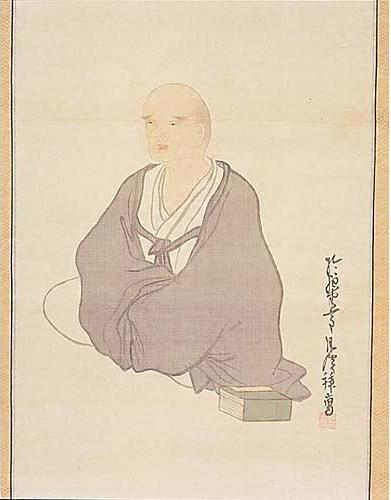
\includegraphics[height=0.9\textheight]{yosa}\\[1em]
        \large{\FS 与谢芜村自画像}
    \end{figure}
\end{center}

\newpage

{\FS
    与谢芜村(1716—1783),本姓谷口,名长庚,字春星,别号宰鸟、夜半翁等。生于摄津国东域郡毛马村(现大阪市都岛区毛马町)富裕的农家。二十岁起,就学俳谐,同时也学绘画。二十九岁时,用「芜村」名(来自陶渊明《归去来辞》的「田园将芜」)。编撰的著作有《玉藻集》、《夜半乐》、《新花摘》等。后期关于俳谐的奥义,曾对他的门人答问说:「用俗语而离俗好,离俗而用俗,离俗法最高。」这与芭蕉的「高悟心而归俗」是相通的。他所谓离俗,是离名利之地,「啸月赏花,游于尘寰之外。」又说「舍风雅而得风雅」,「得句贵在自然」。这些见解是高超的。

    芜村是俳人,也是画家(画南画,笔名子汉,四明,谢寅等)。句中有画,画中有句,崇尚王维。他的俳句,显出浓淡相宜的色彩美,又奇妙地把幻想世界具体化。著名俳人正冈子规对他有很高的评价。他有汉诗的修养,在其名作《春风马堤》\footnotemark[1] 十八首里面,四首用汉诗五言绝句体,所作俳句,也多带有汉诗的格调。作家上田秋成说他是用假名写汉诗的诗人,指出了他的作品的特点。我们可以看到他的诗,有中国的古典作品情趣。

    看来芜村的精神状态,较为乐观畅达,俳句的意境宽阔,而且潇洒华丽,富有浪漫主义色彩,与芭蕉的清寂、细致、质朴无华的现实主义风格,有所差别。他对芭蕉很崇敬,为的是着眼于复兴和提高俳句的艺术性。
}
\footnotetext[1]{\FS 此作乃是寄托归乡途中的女子,怀念久别母亲的心情。}

\newpage

\section{\FK 春}

\setcounter{haikucounter}{0}

\begin{haiku}
    {\FH \ruby[g]{公達}{きんだち}に、\ruby[g]{狐}{きつね}化けたり、\ruby[g]{宵}{よい}の春。}

    {\FK 狐狸变作公子身,灯夜乐游春。}

    {\FT 注:这是怪异俳句。}
\end{haiku}

\begin{haiku}
    {\FH 春の暮、家路に遠き、人ばかり。}

    {\FK 春日黄昏时,尽是远别归家人。}

    {\FT 注:诗人萩原朔太郎说芜村是个乡愁诗人。他写了不少怀乡俳句。}
\end{haiku}

\begin{haiku}
    {\FH ゆく春や、\ruby[g]{逡}{しゆん}\ruby[g]{巡}{じゆん}として、遅ざくら。}

    {\FK 暮春}

    {\FK 春将归去,樱花逡巡而开迟。}

    {\FT 注:原作「逡巡」用汉语。}
\end{haiku}

\begin{haiku}
    {\FH ゆく春や、横河へのぼる、いもの神。}

    {\FK 春将终,天花神,向横河塔攀登。}

    {\FT 注:江户时代,天花流行。母亲们为心爱的儿女担忧。横河塔为比睿山三塔之一。}
\end{haiku}

\begin{haiku}
    {\FH 春\ruby[g]{雨}{さめ}や、\ruby[g]{同車}{どうしゃ}の君が、さざめごと。}

    {\FK 春将归去,与汝同车,低声细语。}

    {\FT 注:汝是女性,典出《史记·孔子世家》卫灵公与夫人同车。}
\end{haiku}

\begin{haiku}
    {\FH \ruby[g]{瀟湘}{しょうしょう}の、雁のなみだや、\ruby[g]{朧}{おぼろ}月。}

    {\FK 春夜闻琴}

    {\FK 潇湘雁落泪,朦胧月色微。}

    {\FT 注:题意出自钱起《归雁》诗:「潇湘何事等闲回?水碧沙明两岸苔。二十五弦弹夜月,不胜清怨却飞来。」}
\end{haiku}

\begin{haiku}
    {\FH 女\ruby[g]{倶}{ぐ}して、\ruby[g]{内裏}{だいり}\ruby[g]{拝}{おが}まん、おぼろ月。}

    {\FK 朦胧月伴美女,同去瞻仰皇居。}

    {\FT 注:写春月的朦胧美,以及艳丽的美女和豪华的皇居。}
\end{haiku}

\begin{haiku}
    {\FH ぬはな\ruby[g]{生}{お}ふ、池の水かさや、春の雨。}

    {\FK 莼菜浮池面,春雨点点。}
\end{haiku}

\begin{haiku}
    {\FH 春雨や、小\ruby[g]{磯}{いそ}の小貝、ぬるるほど。}

    {\FK 春雨细细落,润湿沙滩小贝壳。}
\end{haiku}

\begin{haiku}
    {\FH 滝口に、燈を呼ぶ声や、春の雨。}

    {\FK 春夜雨濛濛,泷口所中,连呼快点灯。}

    {\FT 注:泷口在清凉殿东北,是宫中护卫武士值班所在,这表示发生了什么事故的不安感。}
\end{haiku}

\begin{haiku}
    {\FH 春雨や、ものかたりゆく、蓑と笠。}

    {\FK 春雨里,步行作恳谈,蓑与伞。}

    {\FT 注:蓑指农夫,伞指城市女人,二种身份,竟在春雨中边走边谈,饶有俳画情趣。}
\end{haiku}

\begin{haiku}
    {\FH \ruby[g]{高}{こ}\ruby[g]{麗}{ま}\ruby[g]{舟}{ぶね}の、よらで過ゆく、霞かな。}

    {\FK 高丽船,不靠岸,驶向彩霞天。}
\end{haiku}

\begin{haiku}
    {\FH 指南車を、\ruby[g]{胡}{こ}地に\ruby[g]{引}{ひき}\ruby[g]{去}{さ}る、霞哉。}

    {\FK 指南车入胡地,霞霭里,渐远去。}

    {\FT 注:指南车,中国古代指示方向的车,随后有长驱的大军。《宋史·舆服志》有记载。这句富有异国情调。}
\end{haiku}

\begin{haiku}
    {\FH 春の水、山なき国を、流れけり。}

    {\FK 春水流荡大平原。}

    {\FT 注:此句境界宽阔,气势雄伟。}
\end{haiku}

\begin{haiku}
    {\FH 春の海、\ruby[g]{終日}{ひねもす}のたり、のたり哉。}

    {\FK 春之海,整天荡去漂来。}

    {\FT 注:表示翻复单调的意思,这名句有淡远味。}
\end{haiku}

\begin{haiku}
    {\FH \ruby[g]{藪}{やぶ}入の、夢や\ruby[g]{小豆}{あづき}の、煮えるうち。}

    {\FK 年假省亲梦,就在小豆炊煮中。}

    {\FT 注:此作有《邯郸梦》的味道。}
\end{haiku}

\begin{haiku}
    {\FH \ruby[g]{雉}{きじ}啼や、草の武蔵の、八平氏。}

    {\FK 雉鸟声声啼,武藏野原深草地。想见八平氏。}

    {\FT 注:武藏八平氏,乃武威赫赫的豪族,也不过是一场繁华梦。这和芭蕉的俳句:「长夏草木深,武士当年梦痕」有一样的感慨。}
\end{haiku}

\begin{haiku}
    {\FH 歸る雁、田ごとの月の、曇る夜に。}

    {\FK 归来雁,映田春月朦胧夜。}
\end{haiku}

\begin{haiku}
    {\FH よく聞けば、桶に音を鳴く、田\ruby[g]{螺}{にし}哉。}

    {\FK 若是细细听,桶里田螺有叫声。}
\end{haiku}

\begin{haiku}
    {\FH \ruby[g]{伏勢}{ふくぜい}の、\ruby[g]{錣}{しころ}にとまる、胡蝶かな。}

    {\FK 蝴蝶翩翩,栖息伏兵盔帘上。}

    {\FT 注:蝴蝶飞来,在春野草丛的伏兵头盔上停留。伏兵即伊势平家武士,典出《平家物语》。盔帘日语作「錣」字,即头盔遮住脖子左右和后面的部分。}
\end{haiku}

\begin{haiku}
    {\FH \ruby[g]{釣鐘}{つりがね}に、とまりてねむる、こてふ哉。}

    {\FK 黄蝶停息于吊钟,安然进入梦中。}
\end{haiku}

\begin{haiku}
    {\FH 舟よせて、塩魚買ふや、\ruby[g]{岸}{きし}の梅。}

    {\FK 泊船买盐鱼,梅开满江堤。}
\end{haiku}

\begin{haiku}
    {\FH 白梅に、明くる夜ばかりと、なりにけり。}

    {\FK 初春}

    {\FK 白梅正初开,破晓只为看花来。}

    {\FT 注:写晚年沉浸美的境界和平静清闲的心情,正如许有壬《寻梅》诗所云:「何以慰我衰?梅花秀发时。」这是芜村临终前所吟三句的最后一句。}
\end{haiku}

\begin{haiku}
    {\FH 梅\ruby[g]{遠近}{おちこ}、\ruby[g]{南}{みんなみ}すべく、北すべく。}

    {\FK 远近梅花灿烂,我往北又往南。}
\end{haiku}

\begin{haiku}
    {\FH 白梅や、墨\ruby[g]{芳}{かんば}しき、\ruby[g]{鴻臚館}{こうろくわん}。}

    {\FK 鸿胪馆,白梅翰墨香。}

    {\FT 注:写在鸿胪馆与唐使吟诗作文的交欢。}
\end{haiku}

\begin{haiku}
    {\FH 不二\ruby[g]{颪}{おろし}、十三州の、やなぎかな。}

    {\FK 富士山风飘,十三州里柳枝摇。}

    {\FT 注:十三州指望得见富士山的十三个州。}
\end{haiku}

\begin{haiku}
    {\FH 花の香や、嵯峨のともし火、消る時。}

    {\FK 题花}

    {\FK 嵯峨灯光消失时,犹闻香花气。}
\end{haiku}

\begin{haiku}
    {\FH \ruby[g]{祇}{ぎ}や\ruby[g]{鑑}{かん}や、髭に落花を、\ruby[g]{捻}{ひねり}けり。}

    {\FK 花下联句惜春}

    {\FK 宗祇、宗鉴,捻动须上落花瓣。}

    {\FT 注:宗祇是连歌师,其须有名,山崎宗鉴是俳谐创始人,著有《犬筑波集》。}
\end{haiku}

\begin{haiku}
    {\FH 木の下が、\ruby[g]{蹄}{ひづめ}のかぜや、散さくら。}

    {\FK 风入马蹄轻}

    {\FK 风入蹄轻,树下落樱。}

    {\FT 注:「风入马蹄轻」来自杜甫《房兵曹胡马》「风入四蹄轻」句。}
\end{haiku}

\begin{haiku}
    {\FH 菜の花や、風月は東に、日は西に。}

    {\FK 春景}

    {\FK 一片菜花黄,东有新月,西有夕阳。}

    {\FT 注:写四月菜花盛开的春景。东西的描写,据说来源自陶渊明的「白日沦西河,素月出东岭。遥遥万里辉,荡荡空中景。」}
\end{haiku}

\begin{haiku}
    {\FH 菜の花や、鯨もよらず、海暮ぬ。}

    {\FK 菜花黄似金,鲸鱼离岸不靠近,海上正黄昏。}
\end{haiku}

\section{\FK 夏}

\setcounter{haikucounter}{0}

\begin{haiku}
    {\FH さみだれや、大河を前に、家二軒。}

    {\FK 梅雨不停下,面对大河两户人家。}

    {\FT 注:作者关心百姓人家的生活。}
\end{haiku}

\begin{haiku}
    {\FH ゆふだちや、筆もかはかず、一千言。}

    {\FK 双林寺独吟千句}

    {\FK 骤雨笔酣畅,挥写一千言。}
\end{haiku}

\begin{haiku}
    {\FH 夕だちや、草葉をつかむ、むら雀。}

    {\FK 骤雨蓦然下,群雀猛抓草叶。}
\end{haiku}

\begin{haiku}
    {\FH 夜水とる、里人の声や、夏の月。}

    {\FK 暑天月下人声喧,村民引水入干田。}
\end{haiku}

\begin{haiku}
    {\FH ぬけがけの、浅瀬わたるや、夏の月。}

    {\FK 夏月在天,先骑渡浅滩。}
\end{haiku}

\begin{haiku}
    {\FH 遠浅に、\ruby[g]{兵}{つはもの}舟や、夏の月。}

    {\FK 兵船停海面,夏月挂中天。}

    {\FT 注:白天作战,夜间休息。海上的兵船和空中的月亮,光波交映。}
\end{haiku}

\begin{haiku}
    {\FH \ruby[g]{河童}{かはたろ}の、恋する宿や、夏の月。}

    {\FK 夏天月下,河童钟情人家。}

    {\FT 注:河童是传说中的水怪,嘴尖面如虎。}
\end{haiku}

\begin{haiku}
    {\FH \ruby[g]{揚州}{ようしゅう}の、津も見えそめて、雲の峯。}

    {\FK 初见扬州港,云峰立在天。}

    {\FT 注:这是想象遣唐使到达中国的情景。}
\end{haiku}

\begin{haiku}
    {\FH \ruby[g]{離}{さ}\ruby[g]{別}{ら}れたる、身を\ruby[g]{蹈込}{ふんごん}で、田植哉。}

    {\FK 此身被休离,还是下田插秧去。}

    {\FT 注:写不幸的农村妇女被休后,时值农忙,还是下田,用体力劳动排遣精神上的悲哀。}
\end{haiku}

\begin{haiku}
    {\FH 夕風や、水\ruby[g]{青鷺}{あおさぎ}の、\ruby[g]{脛}{はぎ}をうつ。}

    {\FK 晚风轻轻,波触青鹭胫。}
\end{haiku}

\begin{haiku}
    {\FH \ruby[g]{鮎}{あゆ}くれて、よらで過行、夜半の門。}

    {\FK 留赠我香鱼,夜半悄悄过门去。}

    {\FT 注:鲇,夏季淡水鱼,能吐香气,又名香鱼。钓鲇鱼人为芜村好友,只留赠鲇鱼,过门不入。}
\end{haiku}

\begin{haiku}
    {\FH \ruby[g]{鮒}{ふな}ずしや、\ruby[g]{彦根}{ひこね}が\ruby[g]{城}{しろ}に、雲かかる。}

    {\FK 鲫鱼寿司味好,云绕彦根城堡。}

    {\FT 注:鲫鱼肉发酵后有酸味,将其夹在米饭中的食品,称为鲫鱼寿司,是江州的名产。彦根城是在琵琶湖边山腹的井伊家的城堡。}
\end{haiku}

\begin{haiku}
    {\FH 蚊の声す、\ruby[g]{忍冬}{にんどう}の花の、散るたびに。}

    {\FK 蚊子声细细,正是忍冬花落时。}

    {\FT 注:忍冬,一种蔓草,夏天开花,花色从白变黄,也称金银花。}
\end{haiku}

\begin{haiku}
    {\FH 谷路、行人は小き、若葉哉。}

    {\FK 新叶繁茂,峡谷路上行人少。}
\end{haiku}

\begin{haiku}
    {\FH 浅間山、煙の中の、若葉かな。}

    {\FK 浅间山,弥漫烟中嫩叶鲜。}
\end{haiku}

\begin{haiku}
    {\FH 不二ひとつ、\ruby[g]{埋}{うづ}み残して、わかばかな。}

    {\FK 新绿叶丛淹没中,只余富士一孤峰。}
\end{haiku}

\begin{haiku}
    {\FH 牡丹散りて、打かさなりぬ、二三\ruby[g]{片}{ぺん}。}

    {\FK 牡丹花散,叠地两三片。}
\end{haiku}

\begin{haiku}
    {\FH \ruby[g]{金屏}{きんびょう}の、かくやくとして、牡丹哉。}

    {\FK 金屏风上,牡丹花灿烂。}
\end{haiku}

\begin{haiku}
    {\FH 山\ruby[g]{蟻}{あり}の、あからさま\ruby[g]{也}{なり}、白牡丹。}

    {\FK 一只黑蚂蚁,忽然爬上白牡丹。}

    {\FT 注:一黑一白,色彩鲜明。}
\end{haiku}

\begin{haiku}
    {\FH \ruby[g]{蟻}{ぎ}王宮、朱門を開く、牡丹哉。}

    {\FK 蚁塚}

    {\FK 蚁王宫,牡丹花发朱门红。}

    {\FT 注:取材自李公佐《南柯记》的典故,写出荣华梦景。}
\end{haiku}

\begin{haiku}
    {\FH \ruby[g]{閻王}{えんおう}の、口や牡丹を、\ruby[g]{吐}{ぬ}かんとす。}

    {\FK 波翻舌本吐红莲}

    {\FK 阎王舌片,吐成红牡丹。}

    {\FT 注:标题出典未详。据云《阿弥陀经》有「舌相生红莲」的句子。}
\end{haiku}

\begin{haiku}
    {\FH 花いばら、故郷の路に、似たる哉。}

    {\FK 登东皋}

    {\FK 蔷薇花开处处,恰似故乡路。}

    {\FT 注:作者读陶渊明《归去来兮辞》「登东皋而舒啸,临清流而赋诗」句涌起自己的怀乡情。皋是岸边。蔷薇花的枝干多刺。}
\end{haiku}

\begin{haiku}
    {\FH \ruby[g]{愁}{うれ}ひつつ、岡にのぼれば、花いばら。}

    {\FK 怀愁登古丘,山路野薇幽。}
\end{haiku}

\begin{haiku}
    {\FH 水深く、\ruby[g]{利鎌}{ききかま}鳴らす、眞\ruby[g]{菰}{こも}刈。}

    {\FK 深水割菰蒲,锐利镰刀声。}

    {\FT 注:写爽快的情景。}
\end{haiku}

\begin{haiku}
    {\FH 水桶に、うなづきあふや、\ruby[g]{瓜}{うり}\ruby[g]{茄子}{なすび}。}

    {\FK 香瓜和茄子,相会点头水桶里。}

    {\FT 注:指碰到熟人时的幽默句。}
\end{haiku}

\section{\FK 秋}

\setcounter{haikucounter}{0}

\begin{haiku}
    {\FH 身にしむや、\ruby[g]{亡妻}{なきつま}の\ruby[g]{櫛}{くし}を、\ruby[g]{閨}{ねや}に踏。}

    {\FK 踩了亡妻梳子,感到闺房凉意。}
\end{haiku}

\begin{haiku}
    {\FH 猿どのの、夜寒\ruby[g]{訪}{とひ}ゆく、兎かな。}

    {\FK 秋凉夜,野兔拜访猴爷。}

    {\FT 注:芜村山居,拟鸟羽僧正的鸟兽戏画图作句,富有童话味。}
\end{haiku}

\begin{haiku}
    {\FH 去年より、又さびしいぞ、秋の暮。}

    {\FK 老怀}

    {\FK 又比去年更寂寞,秋之暮。}
\end{haiku}

\begin{haiku}
    {\FH 山鳥の、枝踏みかゆる、夜長哉。}

    {\FK 山鸟踏枝来又去,漫漫长夜里。}
\end{haiku}

\begin{haiku}
    {\FH 月天心、\ruby[g]{貧}{まず}しき町を、通りけり。}

    {\FK 月到天心,人过穷市镇。}

    {\FT 注:北宋邵雍《清夜吟》有「月到天心处」句。穷市镇白天不清洁,夜来被月洗净,欣赏此夜月景。}
\end{haiku}

\begin{haiku}
    {\FH 五六\ruby[g]{升}{しょう}、\ruby[g]{芋}{いも}煮る坊の、月夜哉。}

    {\FK 和尚煮芋五六升,只为今宵赏月明。}

    {\FT 注:一日升,合营造库平制一点七四一升。此是冒充风雅的幽默句。}
\end{haiku}

\begin{haiku}
    {\FH 四五人に、月落ちかかる、おどり哉。}

    {\FK 明月已西沉,舞蹈还有四五人。}

    {\FT 注:盂兰盆节之夜,家家男女集合跳舞,此是看名画家英一蝶(1652—1724)风俗画有感而作。}
\end{haiku}

\begin{haiku}
    {\FH 唐人よ、此花過て、のちの月。}

    {\FK 唐代诗人哟,此花开后还有月。}

    {\FT 注:元稹诗句:「不是花中偏爱菊,此花开尽更无花。」此花指重阳的菊,月指旧历九月十三日夜的月。日人赏月有八月十五仲秋夜,还有九月十三夜。}
\end{haiku}

\begin{haiku}
    {\FH \ruby[g]{唐黍}{とうきび}の、おどろきやすし、秋の風。}

    {\FK 萧簌吹秋风,黍叶易惊动。}

    {\FT 注:此作有汉诗的情趣,南唐李中有「门巷凉秋至,高梧一叶惊」诗句。}
\end{haiku}

\begin{haiku}
    {\FH \ruby[g]{秋風}{しうふう}や、\ruby[g]{酒肆}{しゅし}に\ruby[g]{詩}{し}うたふ、\ruby[g]{漁者}{ぎょしゃ}\ruby[g]{樵者}{せうしゃ}。}

    {\FK 秋风寂寥,酒肆吟诗有渔樵。}
\end{haiku}

\begin{haiku}
    {\FH 鳥羽殿へ、五\ruby[g]{六騎}{ろっき}いそぐ、野分哉。}

    {\FK 落木风天,五六骑,奔向鸟羽殿。}

    {\FT 注:鸟羽殿是鸟羽天皇的离宫。此种情景,表示宫廷将有事变发生。}
\end{haiku}

\begin{haiku}
    {\FH 白露や、茨の\ruby[g]{刺}{はり}に、ひとつづつ。}

    {\FK 荆棘多刺芒,根根闪耀白露光。}
\end{haiku}

\begin{haiku}
    {\FH いなづまや、\ruby[g]{堅田}{かたた}泊りの、宵の空。}

    {\FK 旅宿坚田,电光闪夜天。}

    {\FT 注:坚田在琵琶湖西岸,秋天多电光。}
\end{haiku}

\begin{haiku}
    {\FH いな妻や、佐渡なつかしき、舟便り。}

    {\FK 闪电光中望佐渡,盼船上捎来消息。}
\end{haiku}

\begin{haiku}
    {\FH \ruby[g]{負}{まく}まじき、\ruby[g]{角力}{すまひ}を寝もの、がたり哉。}

    {\FK 角力竞赛输,床上怨内助。}

    {\FT 注:这是写角力者在床上对妻罗唆着他的摔法和不该输掉的道理。相扑到芜村时,在大阪、京都、江户(东京)专业力士定于七月比赛。故相扑成为秋的季语。}
\end{haiku}

\begin{haiku}
    {\FH 鹿寒し、角も身に添ふ、枯木哉。}

    {\FK 角如枯木鹿身寒。}
\end{haiku}

\begin{haiku}
    {\FH 一行の、雁や\ruby[g]{端}{は}山に、月を\ruby[g]{印}{しる}す。}

    {\FK 探题雁字}

    {\FK 雁一行,月印端山上。}
\end{haiku}

\begin{haiku}
    {\FH 釣\ruby[g]{上}{のぼ}し、\ruby[g]{鱸}{すずき}の\ruby[g]{巨}{きょ}口、玉や\ruby[g]{吐}{はく}。}

    {\FK 钓上一尾鲈,巨口吐珍珠。}
\end{haiku}

\begin{haiku}
    {\FH \ruby[g]{沙魚}{はぜ}釣の、小舟\ruby[g]{漕}{こ}ぐなる、窓の前。}

    {\FK 小船钓虾虎,凭窗见摇橹。}

    {\FT 注:虾虎栖在河海之间,秋后钓它。这是在大阪的大川口、隅田川的河口等处水亭上所见的景象。}
\end{haiku}

\begin{haiku}
    {\FH 柳散り、\ruby[g]{清}{し}水\ruby[g]{涸}{かれ}石、\ruby[g]{処々}{ところどころ}。}

    {\FK 柳丝落下水枯涸,河石处处出。}

    {\FT 注:作者爱读苏轼《后赤壁赋》,赏识「山高月小,水落石出」句,奥羽(陆奥、出羽合称,是日本东北六县地区)旅行,写三景并列。}
\end{haiku}

\begin{haiku}
    {\FH 白菊や、呉山の雪を、笠の下。}

    {\FK 旧笠盖菊图}

    {\FK 白菊有如吴山雪,开在草笠下。}

    {\FT 注:宋僧可士句「笠重吴天雪」,「吴天」也用「吴山」。}
\end{haiku}

\begin{haiku}
    {\FH 朝がほや、一輪深き、\ruby[g]{淵}{ふち}のいろ。}

    {\FK 涧水湛如蓝}

    {\FK 牵牛花,一朵深渊色。}

    {\FT 注:标题是宋僧《碧岩录》的句子。}
\end{haiku}

\begin{haiku}
    {\FH 山は暮れて、野は\ruby[g]{黄昏}{たそがれ}の、\ruby[g]{薄}{すすき}哉。}

    {\FK 远山暮霭罩,原野苍茫落日照,蒙蒙狗尾草。}

    {\FT 注:这是芜村名句,为着表现它的境界,试用五、七、五句调译出。}
\end{haiku}

\begin{haiku}
    {\FH 落穂\ruby[g]{拾}{ひろ}ひ、日あたる方へ、あゆみ行。}

    {\FK 对着秋阳,拾穗人步步拾去。}

    {\FT 注:这俳句,正如法国米勒的田园风景画。}
\end{haiku}

\begin{haiku}
    {\FH 秋の燈や、ゆかしき奈良の、道具\ruby[g]{市}{いち}。}

    {\FK 秋夜街灯,奈良可亲旧货市。}
\end{haiku}

\section{\FK 冬}

\setcounter{haikucounter}{0}

\begin{haiku}
    {\FH 水鳥も、見えぬ江わたる、寒さ哉。}

    {\FK 不见浮禽渡江寒。}
\end{haiku}

\begin{haiku}
    {\FH うぐひすの、啼や\ruby[g]{師走}{しわす}の、羅生門。}

    {\FK 莺啼岁暮罗生门。}

    {\FT 注:罗生门为平城京及平安京的正门。平安京的罗生门址在东寺西。这里表示王朝情调的寂静气氛。}
\end{haiku}

\begin{haiku}
    {\FH 寒月や、枯木の中の、竹三竿。}

    {\FK 冬夜月光寒,枯树中间竹三竿。}

    {\FT 注:荒凉的枯树中,还有三枝翠竹映着寒夜月光。}
\end{haiku}

\begin{haiku}
    {\FH 寒月や、\ruby[g]{衆}{しゅ}徒の群議の、過て後。}

    {\FK 寒月映山头,僧兵议战后。}

    {\FT 注:这写属于《太平记》、《平家物语》的世界,比睿山三井寺僧兵在议论明天战事之后。}
\end{haiku}

\begin{haiku}
    {\FH 初雪の、\ruby[g]{底}{そこ}を\ruby[g]{叩}{たたけ}ば、竹の月。}

    {\FK 初雪倾盆落,竹林月色薄。}
\end{haiku}

\begin{haiku}
    {\FH 古池に、\ruby[g]{草履}{ぞうり}沈みて、みぞれ哉。}

    {\FK 古池沉草鞋,雨雪飘飘下。}
\end{haiku}

\begin{haiku}
    {\FH 大雪と、成けり関の、\ruby[g]{鎖}{とざ}し\ruby[g]{時}{ごろ}。}

    {\FK 大雪不停止,关所之门掩闭时。}

    {\FT 注:关所之门为大雪所封闭的情景,使人如见广重的浮世绘。}
\end{haiku}

\begin{haiku}
    {\FH 宿かせと、刀\ruby[g]{投}{なげ}\ruby[g]{出}{だ}す、吹雪哉。}

    {\FK 风雪夜来人,拔刀喊借宿。}

    {\FT 注:写浪人无赖的形象,带有戏剧性。}
\end{haiku}

\begin{haiku}
    {\FH \ruby[g]{凩}{こがらし}や、何に世わたる、家五軒。}

    {\FK 寒风吹得紧,谋生之道何处寻?此地五家人。}

    {\FT 注:写实景,同情穷人。}
\end{haiku}

\begin{haiku}
    {\FH 木枯や、鐘に小石を、吹あてる。}

    {\FK 飕飕寒风,吹起小石碰了钟。}
\end{haiku}

\begin{haiku}
    {\FH 水鳥や、舟に菜を洗ふ、女\ruby[g]{有}{あり}。}

    {\FK 冬川小舟浮,有女洗菜蔬。}
\end{haiku}

\begin{haiku}
    {\FH \ruby[g]{松明}{まつ}ふりて、舟橋わたる、夜の霜。}

    {\FK 松明晃过舟桥,夜霜耀。}
\end{haiku}

\begin{haiku}
    {\FH \ruby[g]{蕭條}{しょうじょう}として、石に日の入、枯野かな。}

    {\FK 荒野萧条不堪,夕阳沉没山石间。}

    {\FT 注:班固有「原野萧条」句,杜甫《望野》诗有「不堪人事日萧条」句,据云为芜村用「萧条」的来源。}
\end{haiku}

\begin{haiku}
    {\FH \ruby[g]{桃源}{とうげん}の、\ruby[g]{路次}{ろし}の細さよ、冬ごもり。}

    {\FK 题诗石上过荒野。}

    {\FK 冬天蛰居,正在桃源路深处。}
\end{haiku}

\begin{haiku}
    {\FH くすり\ruby[g]{喰}{ぐい}、人に\ruby[g]{語}{かた}るな、\ruby[g]{鹿ヶ}{ししが}谷。}

    {\FK 鹿谷吃药事,勿与人提起。}

    {\FT 注:鹿谷在京都左京区,大文字山的西麓。那里有俊宽僧都的山庄。治承元年(1177 年)藤原成亲、康赖等聚集商议讨伐平家而被捕。他们是以吃药食为名义到鹿谷的。药食是指平常嫌它不干净的鹿肉猪肉,冬寒时以为吃了能滋补身体。}
\end{haiku}

\begin{haiku}
    {\FH 枇杷の花、鳥もすさめず、日くれたり。}

    {\FK 日暮枇杷花儿艳,难与鸟儿消遣。}
\end{haiku}

\begin{haiku}
    {\FH \ruby[g]{寒梅}{かんばい}を、手折響や、老が\ruby[g]{肘}{ひじ}。}

    {\FK 寒梅折枝响,联想老胳臂。}

    {\FT 注:把寒瘠的梅枝与老瘦的胳臂作比。}
\end{haiku}

\begin{haiku}
    {\FH 斧入て、香におどろくや、冬\ruby[g]{木立}{こだち}。}

    {\FK 举斧砍枯木,惊异吐香气。}
\end{haiku}

\begin{haiku}
    {\FH 水仙に、狐遊ぶや、宵月夜。}

    {\FK 古丘}

    {\FK 狐狸取乐水仙旁,清冷月夜光。}

    {\FT 注:这是怪异俳句。}
\end{haiku}

\begin{haiku}
    {\FH \ruby[g]{葱}{ねぎ}\ruby[g]{買}{かう}て、枯木の中を、帰りけり。}

    {\FK 买了一把葱,枯林归路中。}

    {\FT 注:冬天菜蔬极少,能够买到新鲜青葱,心情愉快,通过枯木林路回家。青葱与枯木做对比。}
\end{haiku}

\begin{haiku}
    {\FH 我も死して、\ruby[g]{碑}{ひ}に\ruby[g]{辺}{ほとり}せむ、枯尾花。}

    {\FK 芭蕉翁墓前}

    {\FK 我死葬墓旁,亦愿作枯芒。}

    {\FT 注:在京都金福寺谒芭蕉墓后述怀之作。}
\end{haiku}

\chapter[{\FM 小林一茶}]{\FM \ruby[g]{小林}{こばやし}\ruby[g]{一茶}{いっさ}}

\begin{center}
    \begin{figure}
        \centering
        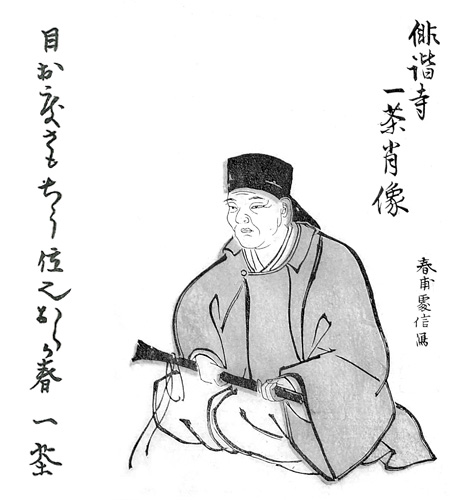
\includegraphics[width=\textwidth]{kobayashi}\\[1em]
        \large{\FS 小林一茶}
    \end{figure}
\end{center}

\newpage

{\FS
    小林一茶(1763—1827),本名弥太郎,生于信浓国水内郡柏原村(今长野县上水内郡信浓町柏原)农民家,三岁母亲去世,八岁来了继母,十岁有了异母弟,他受了虐待。廿五岁到江户,拜二六庵竹阿为师,开始学写俳谐。随后过着流浪生活,离开江户,从京都、大阪赴四国、九州旅行。后来往还于江户与故乡之间。他五十二岁才结婚,所生的三个男孩和一个女孩,均早夭折。六十一岁时,妻死去。六十二岁再娶,不到三个月离婚。六十四岁第三次结婚,留下遗腹女。家乡柏原大火,一茶的家也给烧光,他只好居住在幸存的贮藏室里面。这一年冬天,一茶就在这贮藏室里面逝世。

    一茶的俳句,由于他自己的经历,而形成了他自己的风格。他不大吟风弄月,只吟咏自己及其周围的平凡而不幸的生活,写庄重的句,也写幽默的句,总含点苦味。有人评论一茶,说「自嘲自笑,不是乐天,不是厌世,逸气超然。」他也抒写怀乡之情,他对故乡既有怀念,也有嫌恶的两种感情。他自我暴露,表示卑下无力,但也抒写不平事,却常用幽默和讽刺的手法。他特别慈爱,反对强者,同情弱者,喜爱小动物,对它们好像是好朋友一般亲切。我推测也许和他可悲的童年有关,他得不到家庭的温暖,就亲近乡间的小动物,成为物我一体。这在后来的俳句中充分表现出来。

    另一个是用语的特点,常运用俗语、方言、拟态语、拟声语等,看来像素描画一样。他的学生模仿他的俳风,他却告诫学生说,「我的俳风不可学。」其实没有他的素养和生活感受,也是学不来的。
}

\newpage

\section{\FK 新年}

\setcounter{haikucounter}{0}

\begin{haiku}
    {\FH 元日や、我のみならぬ、巣なし鳥。}

    {\FK 元旦寂寥,不止我是无巢鸟。}
\end{haiku}

\begin{haiku}
    {\FH 元日や、上々\ruby[g]{吉}{きち}の、浅\ruby[g]{黄}{ぎ}空。}

    {\FK 元旦日,大吉大利,浅黄晴空色。}
\end{haiku}

\begin{haiku}
    {\FH \ruby[g]{這}{は}へ笑へ、二つになるぞ、けさからは。}

    {\FK 对两岁的小孩说}

    {\FK 爬吧,笑吧,从今朝起两岁啦!}
\end{haiku}

\begin{haiku}
    {\FH 藪入や、墓の松風、うしろ吹。}

    {\FK 假日回家,坟墓松风身后吹。}

    {\FT 注:假日回家,指男女佣人每年于正月和七月的十六日放假回家。}
\end{haiku}

\begin{haiku}
    {\FH \ruby[g]{逃}{のが}しなや、水祝はるゝ、五十\ruby[g]{聟}{むこ}。}

    {\FK 别让他逃开,被水祝的半百新郎。}

    {\FT 注:水祝,新年亲友到前年结婚的男方家里,泼水祝贺。}
\end{haiku}

\begin{haiku}
    {\FH 舞\ruby[g]{扇}{おうぎ}、猿の涙の、かゝる哉。}

    {\FK 猴子泪水湿舞扇。}

    {\FT 注:作者同情被迫卖艺的猴子。}
\end{haiku}

\begin{haiku}
    {\FH \ruby[g]{垢爪}{あかつめ}や、\ruby[g]{薺}{なずな}の前も、はづかしき。}

    {\FK 人日}

    {\FK 不干净的指甲,在荠菜前,也感到羞惭啊!}

    {\FT 注:人日,中国古时从元旦到正月八日,分为鸡、狗、猪、羊、牛、马、人、谷的日子。正月七日为人日。荠菜,十字花科,春日开花,花小色白,它的嫩茎嫩叶,可供食用,《诗经·邶风·谷风》,有「其甘如荠」句。日本旧俗在人日吃七草粥,内有荠、芹、母子草、佛座、繁缕、芜菁、萝卜七种,以为可除百病,《荆楚岁时记》有记载。荠在人日是吉祥物,指甲沾着荠汁而切荠菜,被认为不干净,故对荠有羞惭之意。\footnote{\FT 日本「春の七草」,用来制作「七草粥」的七种植物,分别是:水芹(芹,せり)、荠菜(荠,なずな)、鼠曲草(古称:御形,ごぎょう;今名:母子草,ははこぐさ)、繁缕(繁缕,古音:はこべら,今音:はこべ),稻槎菜(古名:仏の座,ほとけのざ;今名:小鬼田平子,こおにたびらこ)、芜菁(古名:菘,すずな:今名:芜,かぶ)、萝卜(古名:萝卜,すずしろ;今名:大根,だいこん)。}}
\end{haiku}

\section{\FK 春}

\setcounter{haikucounter}{0}

\begin{haiku}
    {\FH 春雨や、\ruby[g]{喰}{くわ}れ残りの、鴨が鳴。}

    {\FK 春雨纷纷落,吃剩的鸭子叫着。}

    {\FT 注:冬天捕到的野鸭,大多已经吃掉,有的留到春来时还在叫着,被认为是吃剩的。}
\end{haiku}

\begin{haiku}
    {\FH 春めくや、藪ありて雪、ありて雪。}

    {\FK 春意温和,竹林还有积雪,还有积雪。}
\end{haiku}

\begin{haiku}
    {\FH 三\ruby[g]{文}{もん}が、霞見にけり、遠眼鏡。}

    {\FK 白日登汤台}

    {\FK 三文钱租望远镜,望望春霞景。}

    {\FT 注:白日登汤岛天神境内的高台。}
\end{haiku}

\begin{haiku}
    {\FH 西山や、おのれがのるは、どのかすみ。}

    {\FK 西山啊!哪朵云霞乘了我?}

    {\FT 注:经由专明寺主持调停,一茶与异母弟仙六取得和解。于一八一三年春(五十岁)定居故乡,作此喜悦的幽默句。}
\end{haiku}

\begin{haiku}
    {\FH 横乗の、馬のつゞくや、夕がすみ。}

    {\FK 晚霞里,横骑马儿何处去?}

    {\FT 注:写农民忙了一天,在晚霞下,横坐马背上归家。}
\end{haiku}

\begin{haiku}
    {\FH かすむ日や、夕山かげの、\ruby[g]{飴}{あめ}の笛。}

    {\FK 暮色苍茫,山那方,吹笛卖饴糖。}
\end{haiku}

\begin{haiku}
    {\FH \ruby[g]{我庵}{わがいお}や、貧乏がくしの、雪とける。}

    {\FK 掩盖我贫家的雪,已经融解。}

    {\FT 注:信浓雪大,一片白茫茫的雪,盖着房屋,分不清谁是富家,谁是穷家。}
\end{haiku}

\begin{haiku}
    {\FH \ruby[g]{米}{こめ}\ruby[g]{蒔}{ま}くも、罪ぞよ鶏が、けあふぞよ。}

    {\FK 撒把米也是罪过啊!让鸡斗起来。}

    {\FT 注:此句富有理趣,无季语。}
\end{haiku}

\begin{haiku}
    {\FH 亡き母や、海見る\ruby[g]{度}{たび}に、見るたびに。}

    {\FK 想念去世的母亲,当看到海时,看到海时。}

    {\FT 注:五十岁时春三月到千叶富津后,看到大海,感叹自己的流浪,便怀念去世的母亲。此句无季语。}
\end{haiku}

\begin{haiku}
    {\FH 春日のや、あくたれ鹿も、\ruby[g]{角}{つの}落る。}

    {\FK 春日野,鹿角给恶作剧地锯掉。}

    {\FT 注:鹿是奈良春日野神的使者,每年春因防伤人被锯掉。}
\end{haiku}

\begin{haiku}
    {\FH 其夜から、雨に\ruby[g]{逢}{あい}けり、巣立鳥。}

    {\FK 出巢鸟从那一夜起,就碰到落雨。}
\end{haiku}

\begin{haiku}
    {\FH 雀の子、そこのけそこのけ、\ruby[g]{御馬}{おんま}が通る。}

    {\FK 小麻雀,躲开,躲开,马儿就要过来。}
\end{haiku}

\begin{haiku}
    {\FH 我と来て、あそぶや親の、ない雀。}

    {\FK 到我这里来玩哟!没有爹娘的麻雀。}

    {\FT 注:一茶三岁时母亲去世,这是回忆六岁时的吟句,一茶的代表作之一。我觉得文言的译法「孤雀勿哀,与我嬉来」不如用白话表现得更情真意切。}
\end{haiku}

\begin{haiku}
    {\FH 夕燕、我には翌の、あてはなき。}

    {\FK 黄昏燕子有归巢,我没有明天的目标。}

    {\FT 注:这是一茶四十五岁时作,那时居无定所,辗转于上总、下总、常陆之间,故有此感慨。}
\end{haiku}

\begin{haiku}
    {\FH 柳さす、我をさみする、烏哉。}

    {\FK 绿柳枝斜,漠然栖着一乌鸦。}
\end{haiku}

\begin{haiku}
    {\FH \ruby[g]{近江}{おうみ}のや、雁のかへりも、松の月。}

    {\FK 近江归雁松月明。}
\end{haiku}

\begin{haiku}
    {\FH 帰雁、浅間のけぶり、いく度見る。}

    {\FK 归来的雁,见过几回浅间山云烟?}
\end{haiku}

\begin{haiku}
    {\FH \ruby[g]{痩蛙}{やせがえる}、まけるな一茶、\ruby[g]{是}{これ}に有り。}

    {\FK 观斗蛙,四月二十日}

    {\FK 瘦青蛙,别输掉,这里有我一茶!}

    {\FT 注:旧时有斗蛙的习俗。一茶于武藏国(今东京都足立区)竹冢看斗蛙,表示支援弱者。这是一茶的代表作之一。}
\end{haiku}

\begin{haiku}
    {\FH \ruby[g]{悠然}{ゆうぜん}として、山を見る、蛙哉。}

    {\FK 青蛙悠然见南山。}

    {\FT 注:「悠然」是原作用汉语的词儿。}
\end{haiku}

\begin{haiku}
    {\FH とぶ蝶の、人をうるさく、思ふらめ。}

    {\FK 蝴蝶飞远,似不企望这人间。}
\end{haiku}

\begin{haiku}
    {\FH 人\ruby[g]{並}{なみ}に、棚の\ruby[g]{蚕}{かいこ}も、昼寝哉。}

    {\FK 像人一样,棚里的蚕也午睡了。}
\end{haiku}

\begin{haiku}
    {\FH 夕月や、鍋の中にて、鳴田にし。}

    {\FK 黄昏月升时,田螺在锅里啼泣。}
\end{haiku}

\begin{haiku}
    {\FH \ruby[g]{蛤}{はまぐり}の、\ruby[g]{芥}{ごみ}を\ruby[g]{吐}{はか}する、月夜かな。}

    {\FK 月夜里,蚌吐泥。}
\end{haiku}

\begin{haiku}
    {\FH おらが世や、そこらの草も、餅になる。}

    {\FK 生我故乡地,那儿的草,可以做饼哩!}
\end{haiku}

\begin{haiku}
    {\FH 餅になる、草が青むぞ、青むぞよ。}

    {\FK 做饼的草,长青了哩,长青了哩!}

    {\FT 注:可以看到天真的童心,发出惊奇的声调。}
\end{haiku}

\begin{haiku}
    {\FH 梅\ruby[g]{一枝}{ひとえ}、とる人を待、ゆふべ哉。}

    {\FK 黄昏时,等待折梅一枝的人儿。}
\end{haiku}

\begin{haiku}
    {\FH 梅がゝや、どなたが来ても、\ruby[g]{欠}{かけ}茶碗。}

    {\FK 人家去赏香梅,我却谁来也是破茶杯。}
\end{haiku}

\begin{haiku}
    {\FH ゆうゆうと、茨のおくの、野梅哉。}

    {\FK 野薇丛里,野梅悠然开。}
\end{haiku}

\begin{haiku}
    {\FH 茶の煙、柳と共に、そよぐ\ruby[g]{也}{なり}。}

    {\FK 柳枝与茶烟,随风荡漾。}
\end{haiku}

\section{\FK 夏}

\setcounter{haikucounter}{0}

\begin{haiku}
    {\FH 大の字に、寝て涼しさよ、淋しさよ。}

    {\FK 像「大」字一样躺着,又凉爽又无聊。}
\end{haiku}

\begin{haiku}
    {\FH 涼風の、\ruby[g]{曲}{まが}りくねって、来たりけり。}

    {\FK 住里屋}

    {\FK 凉风吹进来,曲折而迂回。}
\end{haiku}

\begin{haiku}
    {\FH \ruby[g]{帰去来}{いざいなん}、江戸は涼みも、むつかしき。}

    {\FK 回家去吧,江户乘凉也难呀!}
\end{haiku}

\begin{haiku}
    {\FH 涼風に、月をも添て、五文哉。}

    {\FK 清风加朗月,五文钱。}

    {\FT 注:是从李白《襄阳歌》「清风朗月不用一钱买」变化来的,李白不用一钱买,一茶却给五文钱。}
\end{haiku}

\begin{haiku}
    {\FH 橋涼し、張良たのむ、此\ruby[g]{沓}{くつ}を。}

    {\FK 桥上凉风吹,张良捡取这鞋来。}

    {\FT 注:典出黄石公在圯上叫张良取鞋的故事。李白有诗《经下邳圯桥怀张子房》。}
\end{haiku}

\begin{haiku}
    {\FH 涼風の、\ruby[g]{浄土}{じょうど}\ruby[g]{則}{すなはち}、我家哉。}

    {\FK 风凉的净土,就是我的房屋。}
\end{haiku}

\begin{haiku}
    {\FH もたいなや、昼寝して聞、田うへ唄。}

    {\FK 粒粒皆辛苦}

    {\FK 万不该啊!午睡时,听唱插秧歌。}

    {\FT 注:标题引用唐李绅《古风》诗句。}
\end{haiku}

\begin{haiku}
    {\FH 五十\ruby[g]{聟}{むこ}、\ruby[g]{天窓}{あたま}をかくす、扇かな。}

    {\FK 五十做新郎,白发扇遮挡。}

    {\FT 注:一茶做新郎时,实是五十二岁,娶二十八岁的菊女为妻。扇为婚礼用品。此作是自我嘲弄。}
\end{haiku}

\begin{haiku}
    {\FH 寝せつけし、子のせんたくや、夏の月。}

    {\FK 孩子已入眠,离屋为他洗尿片,夏月挂天边。}
\end{haiku}

\begin{haiku}
    {\FH 湖水から、\ruby[g]{出現}{しゅつげん}したり、雲の峯。}

    {\FK 真谧静,湖水底下云峰影。}
\end{haiku}

\begin{haiku}
    {\FH \ruby[g]{蝸牛}{かたつむり}、ともども不二へ、上る\ruby[g]{也}{なり}。}

    {\FK 蜗牛一块儿,爬上富士山去也。}

    {\FT 注:写小动物与大高山的对照。比喻集体团结,去完成理想的力量。}
\end{haiku}

\begin{haiku}
    {\FH はらはらと、汗の玉ちる、稲葉哉。}

    {\FK 哗啦哗啦地,汗珠滴落的稻叶。}
\end{haiku}

\begin{haiku}
    {\FH 白雲を、\ruby[g]{袂}{たもと}に入て、\ruby[g]{袷}{あわせ}かな。}

    {\FK 夹袄两袖装白云。}

    {\FT 注:这句从「两袖清风」转化过来的,更饶情趣。}
\end{haiku}

\begin{haiku}
    {\FH 鹿の背に、くすくす鳥の、昼寝哉。}

    {\FK 在奈良}

    {\FK 鹿背上,笑嬉嬉的鸟儿,午睡入梦乡了。}
\end{haiku}

\begin{haiku}
    {\FH 時鳥、何を忘て、引返す。}

    {\FK 布谷鸟,忘记了什么,又转回来?}
\end{haiku}

\begin{haiku}
    {\FH 江戸へいざ、江戸へいざと、時鳥。}

    {\FK 足下也到江户去么?布谷鸟。}
\end{haiku}

\begin{haiku}
    {\FH 前の世の、おれがいとこか、\ruby[g]{閑古鳥}{かんこどり}。}

    {\FK 前生我们是堂兄弟么?布谷鸟。}
\end{haiku}

\begin{haiku}
    {\FH 鳰の巣の、一本草を、たのみ哉。}

    {\FK 䴙䴘的巢,全靠一根草。}

    {\FT 注:巢用芦苇梢端拗折交错而成,浮在水面,也有用零碎的芦苇做成,把巢系在杂草或灯芯草的茎上。}
\end{haiku}

\begin{haiku}
    {\FH 娘見よ、身を\ruby[g]{売}{うら}れつゝ、行蛍。}

    {\FK 女儿看啊,正被卖身去的萤火虫。}

    {\FT 注:夏天有钱人买萤火虫,装在纱袋里,悬在室内,或放在院子里飞翔,以供玩乐。}
\end{haiku}

\begin{haiku}
    {\FH けふの日も、\ruby[g]{棒}{ぼう}ふり虫よ、翌も又。}

    {\FK 日日懈怠,不惜寸阴}

    {\FK 今天是这样,像孑孓游游荡荡,明天也这样。}

    {\FT 注:题用汉文。孑孓是蚊的幼虫。}
\end{haiku}

\begin{haiku}
    {\FH 昼の蚊を、後にかくす、仏かな。}

    {\FK 佛陀将白天的蚊虫,藏在背后。}
\end{haiku}

\begin{haiku}
    {\FH 古郷は、蠅すら人を、さしにけり。}

    {\FK 心所思}

    {\FK 故乡哟,连苍蝇也螫人。}
\end{haiku}

\begin{haiku}
    {\FH やれ打な、蠅が手をすり、足をする。}

    {\FK 别拍打呀,苍蝇手揖脚跪啦!}
\end{haiku}

\begin{haiku}
    {\FH \ruby[g]{蚤}{のみ}の迹、かぞへながらに、添\ruby[g]{乳}{ぢ}哉。}

    {\FK 在喂奶时,又数跳蚤的痕迹。}
\end{haiku}

\begin{haiku}
    {\FH やけ土の、ほかりほかりや、蚤さわぐ。}

    {\FK 火烧场,跳蚤哄哄地乱嚷。}
\end{haiku}

\begin{haiku}
    {\FH 蝉鳴や、空にひつゝく、最上川。}

    {\FK 最上川,蝉声贴在天。}
\end{haiku}

\begin{haiku}
    {\FH 朝やけが、よろこばしいか、蝸牛。}

    {\FK 朝霞红艳艳,蜗牛啊,你可喜欢?}
\end{haiku}

\begin{haiku}
    {\FH 麦秋や、子を\ruby[g]{負}{おひ}ながら、いはし売。}

    {\FK 哀旅贩越后女}

    {\FK 麦秋时节,背着孩子,外出贩卖沙丁鱼。}

    {\FT 注:写越后(今新潟县)妇女的艰苦生活,沙丁鱼是用盐腌的。}
\end{haiku}

\begin{haiku}
    {\FH \ruby[g]{蕗}{ふき}の葉に、いはしを\ruby[g]{配}{くば}る、田植哉。}

    {\FK 每人发一份,款冬叶包沙丁鱼,插秧农忙时。}

    {\FT 注:款冬叶包沙丁鱼,写农村生活的情趣。农忙时,每人分发一份表示慰劳。}
\end{haiku}

\begin{haiku}
    {\FH 初瓜を、引とらまいて、寝た子哉。}

    {\FK 抓着新熟的瓜,睡着的孩子。}
\end{haiku}

\begin{haiku}
    {\FH 塔ばかり、見へて東寺は、夏木立。}

    {\FK 只见五重塔,东寺夏荫遮。}
\end{haiku}

\begin{haiku}
    {\FH 古郷や、よるも\ruby[g]{障}{さは}るも、\ruby[g]{茨}{ばら}の花。}

    {\FK 故乡呀,挨着碰着,都是带刺的花。}
\end{haiku}

\begin{haiku}
    {\FH 昼顔や、ぽっぽと燃る、石ころへ。}

    {\FK 烧热岩石中,旋花欣向荣。}

    {\FT 注:炎夏访喷火后的浅间山麓,赞扬小小花草的生命力。旋花为野生植物,初夏起开淡红色的花,状如牵牛花,午间时盛开,故在日本称昼颜。}
\end{haiku}

\section{\FK 秋}

\setcounter{haikucounter}{0}

\begin{haiku}
    {\FH 秋立や、身はならはしの、よ\ruby[g]{所}{そ}の窓。}

    {\FK 立秋了,站惯别人的窗口外。}
\end{haiku}

\begin{haiku}
    {\FH うそ寒や、\ruby[g]{蚯蚓}{みみず}の唄も、一夜づゝ。}

    {\FK 微寒夜夜里,蚯蚓在唱歌哩。}

    {\FT 注:蚯蚓无发音器官,但作者想象它会唱歌。}
\end{haiku}

\begin{haiku}
    {\FH 秋の夜や、旅の男の、針仕事。}

    {\FK 旅中秋夜里,男人做针线活。}

    {\FT 注:一茶漂泊三十六年,尤其是一七九五年的大旅行,当会有这生活的实感。}
\end{haiku}

\begin{haiku}
    {\FH 我星は、どこに旅寝や、天の川。}

    {\FK 我这颗星,何处寄宿啊?银河。}
\end{haiku}

\begin{haiku}
    {\FH 秋の夜や、窓の小穴が、笛を吹。}

    {\FK 秋夜间,纸窗小破口,吹起笛子响。}
\end{haiku}

\begin{haiku}
    {\FH うつくしや、せうじの穴の、天の川。}

    {\FK 病中}

    {\FK 多美啊!透过纸窗破洞看银河。}
\end{haiku}

\begin{haiku}
    {\FH 木曽山に、\ruby[g]{流}{ながれ}\ruby[g]{入}{いり}けり、天の川。}

    {\FK 银河倾泻木曾山。}

    {\FT 注:木曾山可能在一茶故乡信浓境内,指木曾诸山。木曾在今长野县西南部,木曾川上游山谷地乃桧木产地。此句写沉郁静美的夜空。}
\end{haiku}

\begin{haiku}
    {\FH 又人に、かけ\ruby[g]{抜}{ぬか}れけり、秋の暮。}

    {\FK 秋日黄昏行脚里,后面有人赶前去。}
\end{haiku}

\begin{haiku}
    {\FH たまに来た、古郷の月は、曇りけり。}

    {\FK 偶尔回家转,故乡的月色暗淡。}
\end{haiku}

\begin{haiku}
    {\FH 名月を、さしてかまはぬ、草家哉。}

    {\FK 如明月之所见,我的破家园。}
\end{haiku}

\begin{haiku}
    {\FH あの月を、とってくれろと、泣子哉。}

    {\FK 小孩哭着嚷,要取那月亮。}
\end{haiku}

\begin{haiku}
    {\FH 名月や、けふはあなたも、いそがしき。}

    {\FK 明月呀,今天你也贵忙。}

    {\FT 注:用「你」使人感觉亲切,想到月亮移行很快。}
\end{haiku}

\begin{haiku}
    {\FH \ruby[g]{義経}{よしつね}は、松の月さへ、ひいき哉。}

    {\FK 源义经,松月也对他表同情。}

    {\FT 注:源义经战功显赫,终为其兄源赖朝所不容,此句写出松月对义经也寄写同情。}
\end{haiku}

\begin{haiku}
    {\FH 同じ年の、顔の\ruby[g]{皺}{しわ}見ゆる、灯籠哉。}

    {\FK 灯笼啊,照见同年人的皱容。}
\end{haiku}

\begin{haiku}
    {\FH 案山子にも、うしろ向かれし、\ruby[g]{栖}{すみか}哉。}

    {\FK 我的家呀,稻草人也不理睬。}

    {\FT 注:写回乡后不顺心。稻草人是秋的季语。}
\end{haiku}

\begin{haiku}
    {\FH 馬の子の、故郷はなるゝ、秋の雨。}

    {\FK 秋雨绵绵,小马卖出离故乡。}
\end{haiku}

\begin{haiku}
    {\FH なくな雁、けふから我も、旅人ぞ。}

    {\FK 雁别叫了,从今天起,我也是漂泊者啊!}
\end{haiku}

\begin{haiku}
    {\FH 田の雁や、里の人数は、けふもへる。}

    {\FK 田里雁声叫,村中人见少。}

    {\FT 注:人见少,指信浓的旧俗,从晚秋到春天,壮年人出外谋生。}
\end{haiku}

\begin{haiku}
    {\FH 秋風に、歩行て逃る、蛍哉。}

    {\FK 萤火虫,步行潜逃避秋风。}

    {\FT 注:秋来了,萤火虫已经衰弱无力,以步行来表现它。作者自况。}
\end{haiku}

\begin{haiku}
    {\FH \ruby[g]{仰}{あう}のけに、寝て鳴にけり、秋の蝉。}

    {\FK 秋天的知了,仰卧地上向天叫。}
\end{haiku}

\begin{haiku}
    {\FH 秋風や、むしりたがりし、赤い花。}

    {\FK 长女莎托墓前}

    {\FK 秋风呀,小红花,要被撕碎了的!}

    {\FT 注:一茶的长女生于一八一八年五月四日,翌年患痘疮,于六月二十一日死。}
\end{haiku}

\begin{haiku}
    {\FH 蟷螂が、不二の\ruby[g]{麓}{ふもと}に、かゝる哉。}

    {\FK 螳螂爬到富士山麓。}
\end{haiku}

\begin{haiku}
    {\FH 人をとる、茸はたして、うつくしき。}

    {\FK 毒蘑菇}

    {\FK 害人的蘑菇,果然很娇妩。}
\end{haiku}

\begin{haiku}
    {\FH 夕暮に、むしろちれちれ、菊の花。}

    {\FK 夕阳落脚下,地上野菊花。}
\end{haiku}

\section{\FK 冬}

\setcounter{haikucounter}{0}

\begin{haiku}
    {\FH \ruby[g]{椋}{むく}鳥と、人に呼るゝ、寒哉。}

    {\FK 往东国途中}

    {\FK 人们呼唤白头翁,感到寒气重。}

    {\FT 注:东国指关东地区。信浓的白头翁鸟出现在寒冬时节。一茶五十岁时在《七番日记》中说自己是白头翁,这里人与鸟是相关的。}
\end{haiku}

\begin{haiku}
    {\FH 次の間の、灯で飯を喰ふ、夜寒哉。}

    {\FK 孤身旅行}

    {\FK 隔壁自进餐,灯暗风又寒。}
\end{haiku}

\begin{haiku}
    {\FH \ruby[g]{朝晴}{あさばれ}に、ぱちぱち\ruby[g]{炭}{すみ}の、きげん哉。}

    {\FK 早晨晴朗,火炭毕毕剥剥好舒畅。}
\end{haiku}

\begin{haiku}
    {\FH 行としや、空の青さに、守\ruby[g]{谷}{や}迄。}

    {\FK 廿三日入西林寺}

    {\FK 辞岁青空下,步行到守谷。}

    {\FT 注:一茶于一八一〇年十二月入守谷西林寺。守谷今茨城县北相马郡守谷町。}
\end{haiku}

\begin{haiku}
    {\FH 人並に、正月を待つ、灯影かな。}

    {\FK 像普通人,灯火期待新春。}
\end{haiku}

\begin{haiku}
    {\FH \ruby[g]{業}{ごう}の鳥、罠を巡るや、むら時雨。}

    {\FK 强盗藏在我的故乡被捕}

    {\FK 村间雨落,作孽的鸟,陷入圈套。}
\end{haiku}

\begin{haiku}
    {\FH しぐるゝや、芭蕉\ruby[g]{翁}{おきな}の、塚まはり。}

    {\FK 冬天的雨呀,绕着芭蕉翁的墓地。}
\end{haiku}

\begin{haiku}
    {\FH 木がらしや、\ruby[g]{地}{じ}びたに暮るゝ、辻\ruby[g]{諷}{うた}ひ。}

    {\FK 人生道路比山川还艰险}

    {\FK 寒风飘摇日将暮,有人卖唱十字路。}
\end{haiku}

\begin{haiku}
    {\FH 行人を、\ruby[g]{皿}{さら}でまねくや、薬喰。}

    {\FK 用碟子招呼行人,尝尝药食品。}

    {\FT 注:药食品是由鹿肉配药材煮成的。}
\end{haiku}

\begin{haiku}
    {\FH あゝまゝよ、年が暮よと、くれまいと。}

    {\FK 在此年关下,不管是好还是歹,任凭你安排。}
\end{haiku}

\begin{haiku}
    {\FH 心から、\ruby[g]{信濃}{しなの}の雪に、降られけり。}

    {\FK 信浓的雪,从心头落下。}

    {\FT 注:指家乡的人情淡薄,这里的雪成为袭击生活的东西,与风雅咏雪,全然异趣。}
\end{haiku}

\begin{haiku}
    {\FH うまさふな、雪やふふはり、ふふはりと。}

    {\FK 许是好吃的雪花,乱纷纷地飘下。}
\end{haiku}

\begin{haiku}
    {\FH 是がまあ、つひの栖か、雪五尺。}

    {\FK 十二月廿四日入故乡}

    {\FK 这终老住居地,哦,雪五尺!}

    {\FT 注:《八番日记》记每年要开支一笔扫雪费。一茶住这雪国,据统计写雪俳句有四百多首。此句是一八一二年(五十岁)写的。}
\end{haiku}

\begin{haiku}
    {\FH 真直な、小便穴や、門の雪。}

    {\FK 门前雪,小便洞真直}

    {\FT 注:这句有点卑俗,是生活的实感。蕉门其角也有这么个句子:「初雪里,这小便是哪个小子的?」}
\end{haiku}

\begin{haiku}
    {\FH 野仏の、御鼻の先の、\ruby[g]{氷柱}{つらら}哉。}

    {\FK 野佛鼻梁挂冰柱。}
\end{haiku}

\begin{haiku}
    {\FH 母親を、霜よけにして、寝た子哉。}

    {\FK 睡着的孩子,将母亲当防霜帘子}
\end{haiku}

\begin{haiku}
    {\FH 冬籠る、蛇の隣や、鼠穴。}

    {\FK 蛇蛰居过冬,邻家便是老鼠洞。}
\end{haiku}

\begin{haiku}
    {\FH \ruby[g]{象潟}{きさかた}の、欠をかぞへて、鳴千鳥。}

    {\FK 鸟海山埋海里,千满寺入地底}

    {\FK 象潟的千鸟,抓着破片啼叫。}

    {\FT 注:鸟海山,羽前羽后之间的名山,又称出羽富士。千满寺,即象潟的千满珠寺。千鸟是候鸟,嘴尖体小,背黑腹白,尾短腿长,冬天群集河、海上。千鸟,冬的季语。象潟曾于一八〇四年遭过地震,标题写出了地震的毁灭力。芭蕉《奥川小道》说游过此地。一茶不知何时到奥羽旅行,写下这真实的印象。}
\end{haiku}

\begin{haiku}
    {\FH 大根引、大根で道を、教へけり。}

    {\FK 拔萝卜的,拿着萝卜指路。}

    {\FT 注:写朴素的田园风景,活现指路人形象,还可想见有个问路人。}
\end{haiku}

\begin{haiku}
    {\FH \ruby[g]{焚}{た}くほどは、風がくれたる、おち葉哉。}

    {\FK 燃料够了,风送来的落叶。}

    {\FT 注:这是名作。}
\end{haiku}

\begin{haiku}
    {\FH こやし\ruby[g]{積}{つむ}、夕山\ruby[g]{畠}{ばた}や、散紅葉。}

    {\FK 粪肥堆叠,夕暮山田散红叶。}

    {\FT 注:红叶经晚秋、初冬的风雨而凋落,称散红叶或残红叶,属冬红叶一类。}
\end{haiku}

\begin{haiku}
    {\FH 家ありて、そして水仙、畠かな。}

    {\FK 有个家,再建个水仙园吧。}
\end{haiku}

\chapter[{\FS 寻钟声的余韵(代跋)}]{\FS 寻钟声的余韵(代跋)\\\hspace{2em}——俳句学习笔记}

 {\FS
  中日两国是近邻,自古就有诗文的交流。虽说是同文,但日本的语文,与中国的语文,仍有差别。学习这种日本特有短诗体俳句(HAIKU),我的理解,却是个中国人的门外俳谈。

  对于俳句,引起我的注意和兴趣的,说来有三点原因:一,它在日本文学史占有重要位置;二,直到现代仍然拥有广泛的群众基础;三,在国际诗歌界,也有它的影响。我明知研究俳句,有很大的难度,也硬着头皮去学习它,琢磨它。我谈不上有什么心得,总是觉得俳句那么短,却能够写景、抒情等,有它的表现力。短是它的特点。如所周知,越短的诗体,就越难写,它贵含蓄、重暗示,要有言外之意,弦外之音,留有余韵,能给读者吟味。「情融乎内而深且长,景耀乎外而远且大」。(方东树《昭昧詹言》)要求如《文心雕龙·神思篇》所说:「寂然凝虑,思接千载,悄焉动容,视通万里」,做到作品短小,而境界时空长远。

  关于俳句的艺术感染力,小泉八云氏曾有恰好的比喻,他以为最好的短诗,正如寺钟的一击,使缕缕的幽玄的余韵,在听者的心中永续地波动。我们欣赏秀逸的俳句,也就是像在寻求钟声悠长的妙韵。

  \section*{\FS 季语的理解}

  关于四季的景物,陶渊明写道:「春水满四泽,夏云多奇峰,秋月扬明晖,冬岭秀孤松。」四时景物,不断变化,人的心情也受到感染。于是,陆机《文赋》把情思和四季景物交融时,写道:「遵四时以叹逝,瞻万物而思纷。悲落叶于劲秋,喜柔条(柳)于芳春,心懔懔以怀霜,志渺渺而临云。」陆机的说明,与弘法大师《文镜秘府论·论文意》说:「春夏秋冬气色,随时立意。」和芭蕉所说:「乾坤的变化,乃风雅的种子。」(《三册子·赤》)「随顺造化,与四时为友」,(《书箱小文》)有着近似点。

  季语是俳句结构的要素,俳句有季语,增加句的姿色美,成为审美的传统习惯。从这里看到日本人对岁时季节的敏感,这也许与岛国的天文、地理和农渔业有关。
  季语,大体可以分为二类:一是自然现象,即时令,风月云雪,鸟兽鱼虫和花木草等,二是社会现象,如宗教、人事(忌日纪念)等。随着社会生活的演变,人事季语也会增加季语在句中的作用,有的是成为主题的配景,有的表现为主要的直接的主题,作者从这主客观关系中抒发感情。

  从古典俳句中,粗略分析一下,看来写自然的多,写社会的少;写景的多,抒情的少。当然也不可机械地分开,大量主要的俳句,写得情景交融难分,其中也有的含着一种理趣。

  季语,广义地说也是景语(这个词儿,《文镜秘府论》用过),景语与情语不免会发生接触,即从自然界及社会上的客观景象和作者主观感情的交融,从各种感观通到心灵,触景生情;或是移情入景,即作者选择适合抒情的景物,以至化无情的景物为有情,使客观的景物,变为主观思想感情加工了的景物。

  \section*{\FS 意境}

  从季语使我想到意境。

  《文镜秘府论·论文意》写道:「夫置意作诗,即须凝心目击其物,便以心击之,深穿其境。」这就早已说明意与境的联系。意境论在诗学是重要的课题。松尾芭蕉曾谈到「写松学松,写竹学竹」的话,意思也有要求作者的情意渗入松竹的意味。到后来竟达到「物我一如」的境界,说「物我分为二,其情即不真诚。」(见《三册子·赤》)这种精辟的俳论,和我国王国维《人间词话》所说:「能写真景物,真感情者,谓之有境界。」袁枚的「性灵论」,也有对诗要求真实情感的见解,中日诗家关于意境的观点,多么地吻合。

  关于意境的表现形态,是主客观的相互融合,主要可分两类;一是触景生情,一是移情入景,后一类发展到物我一如。请让我举些例子说明吧:

  触景生情,表示由景影响情,《文心雕龙·物色篇》说:「春秋代序,阴阳惨舒,物色之动,心亦摇焉。」如王昌龄《闺怨》:「忽见陌头杨柳色,悔教夫婿觅封侯。」又如《渡易水歌》:「风萧萧兮易水寒,壮士一去兮不复还。」

  下列的俳句,是同样作法:

  \begin{quote}
      听得猿声悲,秋风又传弃儿啼,谁个最惨凄?\hfill 芭蕉

      长夏草木深,武士当年梦痕。\hfill 芭蕉

      踩了亡妻梳子,感到闺房凉意。\hfill 芜村

      黄昏燕子有归巢,我没有明天的目标。\hfill 一茶
  \end{quote}

  移情入景,诗人把自己真实、深沉的感情,注入景物中而抒发出来「情哀则景哀,情乐则景乐。」这是诗人不仅写景,也是造景,所谓季语,属于景语,也变为情语了。如杜甫《春望》「感时花溅泪,恨别鸟惊心。」诗人笔下的花鸟在这里化为溅泪的花和惊心的鸟了。

  \begin{quote}
      蚌壳蚌肉苦分离,秋将归去时。\hfill 芭蕉
  \end{quote}

  芭蕉把别离亲人的苦痛,以蚌的壳和肉体分开来表现。

  \begin{quote}
      寒风吹得紧,谋生之道何处寻?此地五家人。\hfill 芜村

      梅雨不停下,面对大河两户人家。\hfill 芜村
  \end{quote}

  这后句,可说并非单纯写景,在梅雨淋漓,大河激流汹涌时,作者与前句关心五家人一样,对着岸畔小小两户人家,倾注关切之情。

  \begin{quote}
      瘦青蛙,别输掉,这里有我一茶!\hfill 一茶
  \end{quote}

  移情入景,是情景相生形成深度,达到物我一如的境地,看来彼此亲密无间,成为一体了。试看下列作者与禽鸟关系的句子。李白《奔亡道中》:「谁忍子规鸟,连声向我啼」的诗句,和芭蕉下面的句子也有近似之处。

  \begin{quote}
      让忧郁的我寂寞吧,子规鸟!\hfill 芭蕉
  \end{quote}

  此外还有:
  \begin{quote}
      到我这里来玩哟!没有爹娘的麻雀。\hfill 一茶
  \end{quote}

  南宋词人辛弃疾,要和鸥鹭结盟,他在《水调歌头·盟鸥》中写道:「凡我同盟鸥鹭,今日既盟之后,来往莫相猜。白鹤去何处,尝试与偕来。」

  李白还有这类境界的诗句,他不止一次要和海鸥同游,《赠王判官时余归隐居庐山屏风叠》:「明朝拂衣去,永与海鸥群。」辛弃疾说:「谪仙人,鸥鸟伴,两忘机。」杜甫《春水生》也有「鸬鹚鸂鶒莫漫喜,吾与汝曹俱眼明。」

  \section*{\FS 虚实}

  虚实也是一种写法,实中有虚、虚中有实;实非实,虚非虚等形式,大体上实指景物,虚指情思,也指有形物与无形物之别。在汉语中,有一种化实为虚,写法有变化,境界就觉得宽些,余味觉得长些,例如刘长卿《新年作》,有「岭猿(实)同旦暮(虚),江柳(实)共风烟(虚)。」李白的「桃花潭水深千尺(实),不及汪伦送我情(虚)。」芭蕉也有实中有虚的句,如:

  \begin{quote}
      时鸟声横江水上。\hfill 芭蕉

      夏月夜,章鱼壶中虚幻梦。\hfill 芭蕉

      举斧砍枯木,惊异吐香气。\hfill 芜村
  \end{quote}

  与此相反,是变虚为实的句法,如白居易《夜筝》的「别有深情(虚)千万重(实)。」张旭《山中留客》的「纵使晴明无雨色(虚),入云深处亦沾衣(实)。」在古典俳句中,也有虚中有实的句子。如:

  \begin{quote}
      静寂,蝉声入岩石。\hfill 芭蕉
  \end{quote}

  无形的蝉声,渗入有形的岩石,使人想象那种境界,惊叹他写出静寂到如此的深度。

  \begin{quote}
      年假省亲梦,就在小豆炊煮中。\hfill 芜村
  \end{quote}

  这与《黄梁梦》的情节近似,从虚到实,醒来一场空,也能使人回味。

  \begin{quote}
      元旦寂寥,不止我是无巢鸟。\hfill 一茶
  \end{quote}

  元旦的漂泊的苦情,用无巢鸟来作比,更具体生动。

  在俳句与汉诗的写法上,从实到实的作品很多,因写实是基本的创作方法。从虚到虚就较少见。至于实非实,则近乎虚;虚非虚,则近乎实,两者是有瓜葛的。要寻句例,一时只想到有以下句子:

  \begin{quote}
      最上川,蝉声贴在天。\hfill 一茶
  \end{quote}

  蝉声是有声无形,天有形而虚空,说它实却非实,说它虚却非虚。这种句,还是有它的味道的。景语中的季语,看来是实。实与虚,如景物与情思交融,可以转化。这全靠作者的功力,要有丰富的想象力,有鲜明的形象感,巧妙的排比组合,使作品成为令人寻味的意境。

  芜村那些怪异的俳句,如以狐狸为题材的俳句,使我想到我们名作《聊斋》中的故事,虽属虚构,读来形象是逼真的,它带有浪漫主义的色彩。

  \section*{\FS 时间}

  因为俳句形体短小,容易产生内容(写景或抒情)是一瞬间的事,的确,有这样的句,而且不少是名句。如

  \begin{quote}
      古池塘呀,青蛙跳入水声响。\hfill 芭蕉
  \end{quote}

  这句的时间,只在跳入的一瞬间。

  \begin{quote}
      菜花一片黄,东有新月,西有夕阳。\hfill 芜村
  \end{quote}

  这也是抓住地球转动,日月相见的那个短时间。又如前引的「瘦青蛙,别输掉,这里有我一茶」(一茶)也是抓住斗蛙那个时间内对瘦青蛙的感情。

  我们不能抓住这一点,不管其他,便加以论断。俳句中写长时间的句,比比皆是。我们可以举例证说明

  \begin{quote}
      长夏草木深,武士当年梦痕。\hfill 芭蕉
  \end{quote}

  感慨历史的事件,时间是较长的,芜村也有不少相类似的句子。

  \begin{quote}
      春之海,整天荡去又飘来。\hfill 芜村
  \end{quote}

  写荡去飘来海的形象,是整个春天的长时间。

  \begin{quote}
      这终老住居地,哦,雪五尺!\hfill 一茶
  \end{quote}

  写终老地的五尺厚的雪,概括相当长的冬天。

  俳句内容时间的一瞬,与作者凭灵感作句的一瞬,范畴不同。时间的短暂与时间的持续,犹如点与线的关系。于此间,又产生时间与空间联系的问题,没有时间的空间,没有空间的时间,是不存在的。

  拿上面的例子说,「古池塘呀,青蛙跳入水声响。」空间是古池塘,比较狭窄。而「菜花一片黄,东有新月,西有夕阳。」空间就十分辽阔。

  中国诗词的句子,在同一个时间内,空间却排列多种景象。这两个例子,没有谓语,以清晨的景象表达作者的情思。
  \begin{quote}
      温庭筠《商山早行》「鸡声茅店月,人迹板桥霜。」

      柳永《雨霖铃》「杨柳岸,晓风残月。」
  \end{quote}

  中日诗歌一样,有的句子,先说时后说空;有的句先说空后说时,时空难以划清界线。如:

  \begin{quote}
      江户客居已十霜,便指是故乡。\hfill 芭蕉

      牛棚残暑蚊声暗。\hfill 芭蕉
  \end{quote}

  岑参《馆中作》的「今夜不知何处宿,平沙万里绝人烟」,这是先时后空;《首秋轮台》的「轮台万里地,无事历三年」,这是先空后时。

  由于岁月流逝,一去不回,「俯仰之间,即成陈迹」,不免感慨系之。芭蕉也曾引用李白的「天地者万物之逆旅,光阴者百代之过客」的观点。在他的吟咏中,有的是感伤,用拟人法。如:

  \begin{quote}
      春将归,鸟啼鱼落泪。

      一年又一年,叫猴戴假面。
  \end{quote}

  有的表示佛家无常观,如:

  \begin{quote}
      知了在叫,不知死期已到。

      路旁木槿花,马儿一口吃掉它。
  \end{quote}

  一茶因自己的妻子和女儿的病亡,感伤和无常观表现得更明显。

  汉诗中,如陈子昂《登幽州台歌》,吊古伤今,慷慨悲歌,富有感染力,抄之如下:

  \begin{center}
      前不见古人,

      后不见来者,

      念天地之悠悠,

      独怆然而涕下。
  \end{center}

  至于含有无常观的,如白居易的偈语似的佛理诗,其中就有这种味道。芭蕉的马吃掉木槿花句和白居易的「木槿一日自为荣」,李义山的「可怜荣落在朝昏」,是有牵联的。

  \section*{\FS 通感}

  在诗歌中,有一种表现的手法或修辞,就是在视觉、听觉、嗅觉、触觉和味觉中,把两个感官相通了,叫做「通感」。

  我读芭蕉的俳句集,就接触到一些通感的句子。例如:

  \begin{quote}
      松风落叶水声凉。

      海边暮霭色,野鸭声微白。

      比起石山石,秋风色更白。

      残暑牛棚蚊声暗。
  \end{quote}

  芭蕉写出鸭声白,中国诗人叫作「听声类形」,如李世熊《寒支初集卷一·剑浦陆发次林守一》诗句,有「月凉梦破鸡声白」,这也可说是一种偶合吧。其他中国诗人也有通感的表现手法,如李白写雪发出香气的诗句「瑶台雪花数千点,片片吹落春风香。」杜甫写竹发出香气的诗句「雨洗涓涓净,风吹细细香」,都是把视觉和嗅觉沟通起来,对不香的东西,说它香。诗笔补了自然景物之不足,使自然景物更加美好。西欧诗人也有这种通感的表现法。初看起来,是颇费解的。

  \section*{\FS 关于俳句试译}

  松尾芭蕉、与谢芜村、小林一茶这三位俳人在日本文学史上享有声誉。因为俳句难懂,也就难译,即使看得懂,也难译得好,所以历来极少翻译,因此中国读者对俳句,不大了解。从文化交流看来,彼此介绍对方国家的名作,也是重要的工作。

  承蒙日本俳人朋友赠送关于俳句的书籍,我学习之后,才有初步的理会,竟不量力,动起试译的念头。在翻译工作过程中,必然感到有许多困难。上述三位古典俳人,作品很多,不免要经过一番选择。凭我的偏见,就按以下三个标准:一,意境别致,感情真挚,艺术手法较高的;二,能够反映社会生活,并有一定情调和理趣的;三,可以看到和汉诗的某种联系的。至于宗教气味浓厚或人情风俗及其事物,不容易为我们读者所领会的,怕注释一多,读来乏味,只好割爱。

  日语是复音,汉语是单音,语言还有各自的特点,如樱在日语是三个音,莺是四个音,所以十七音的俳句,不能按五、七、五三行的办法来译,因为这样容易增加原作所无的许多字面,致使有「说尽」或「说过头」的毛病。除非有些俳句,如不增加点字面,不能使俳句所写的事物联系起来,影响达意传神,才不得已添加一些。

  \begin{quote}
      黄鹂声声啭,听来刚在翠柳后,又在竹枝前。\hfill 芭蕉
  \end{quote}

  原句是侧重听觉的,这不算增加什么东西吧。有的俳句,实际上用七个字,似乎也就可以表达原意,不必「画蛇添足」。例如:

  \begin{quote}
      角如枯木鹿身寒。\hfill 芜村
  \end{quote}

  但这里产生一个值得研究的问题。就是单独一句七言诗,不能成为一首诗。即使是脍炙人口的名句也只能当作断句。这从音调上说来,七音比十七音,可能单调促迫些。如「山雨欲来风满楼」,从意境说来,它是能够展开去的,不必用别句帮助,但也不能成为一首诗。此外,还有由于民族、时代的不同,读者的审美观不同,在日本公认是佳句,未必能译得好,纵然译得不错,也未必能引起读者的同感叫好。

  上述三位俳人的俳句,有各自的风格,非加注意不可,芭蕉、芜村,还可以用文言翻译,而一茶的很多作品是和小动物对话,则非用白话不可。翻译诗歌,贵在神似,借体投魂,非常困难。「信达雅」,那是努力的目的,我想如能以简炼字面,和谐句调,传出原作的神情,那就算可取的了。把日本俳句的格调汉诗化,这不是思想上的民族自大,而是艺术上照顾读者的审美习惯。

  译法问题,是个难题,不仅要有好理论做指导,还要译作实践跟上去,这是值得深入研究讨论的问题。

  \section*{\FS 关于汉俳试作}

  朋友们曾询问过我,为什么写起汉俳(中国式俳句)来?我一时回答不出来,不过想了一下,觉得我学习写诗,已经多年,由于读过俳句,和俳人往来,就引起了兴趣。既然有诗人学西欧商籁体,写十四行诗,我们也可以学日本俳句,写三行诗。这是文学交流的产品,也是「以文会友」之道。

  欧美的诗人,也早就试写俳句体的三行诗,至今仍有人在写。我国当前的诗坛,有人评论说诗有越写越长(并非叙事诗)的倾向,重量不重质。这是个问题,有必要要求诗写得短些好些。那么,汉俳只是三行诗,也可以试作。在我看来,抓住一时感兴,写出三行,比写四行的绝句,更自由些。一九八一年就把赵朴初、钟敬文、公木、陈大远、袁鹰等同志和我写的,编集在《诗刊》、《人民日报》发表,算是汉俳的幼苗从此出土和读者初次见面了。

  既然叫做汉俳,当然与俳句有关,不能只按形式上五、七、五音节,同时也须注意俳句的艺术特点。因为汉语是单音,日语是复音,中国的十七音比日本的十七音,内容意思就多了,这就得照顾我国读者对汉语三行诗审美的习惯。如果把三行汉俳译成俳句,那就不是一首俳句所能容纳的。两者之间,还有所差异。

  俳句有「季语」,它被用在上五或下五,也有用在中七的;汉俳也就不能不关照这点。但每首汉俳,都要有「季语」,也不是容易的事。

  我有一种护短的观点,与其把季语,当作起兴,或作配景,不能集中抒情,或写出情调或理趣来,似乎也可以不必硬用。下面一茶这理趣式的俳句,就没有季语:

  \begin{quote}
      撒把米也是罪过啊,让鸡斗起来。
  \end{quote}

  日本川柳也和俳句一样十七音,它用俗语,歌咏讥讽世俗人情,却不用季语。我想,如果写的社会性生活题材越多,使用季语也会越难的吧?

  从俳句产生汉俳,使中日诗歌界人士,由于同好,更加亲切,并扩大了影响。使我难忘的是一九八一年春,我和袁鹰同志应日本俳人协会的邀请,曾在京都平安神宫观赏樱花时,俳人协会会长大野林火先生以樱花命题,要各自写一首俳句或汉俳,名俳人山口誓子写下了如下的俳句:

  \begin{center}
      樱花凝红艳,

      胜过楼阁朱丹。
  \end{center}

  我为樱花的美所迷醉,于是写了如下的汉俳:

  \begin{center}
      花色满天春,

      但愿剪得一片云,

      裁作锦衣裙。
  \end{center}

  大野林火先生为这首汉俳,在报刊作了介绍和解释,至今我仍怀谢意。

  日本俳句虽然不像汉语存在平仄、押韵的问题,但也要求顺口的音乐性,因此大多汉俳押韵、或押相近的韵。其实也可以用白话,不押韵。钟敬文教授用口语写的汉俳,根本不押韵,只用季语因有俳句的异国情调,读来也有味,就抄一首在这里吧,题是《错过》:

  \begin{center}
      花事到荼蘼,

      又错过赏春时节,

      且待来年罢。
  \end{center}

  汉俳是中日文化交流中新的短诗体,仍在试作中,关心的同志日益增多,我们盼望这个队伍逐步扩大起来。

  \bigskip

  附记:这篇俳句学习笔记,是应日本《俳句》杂志之约写的。

  \hfill 一九八二年七月初
 }

%!TEX root = haiku.tex
\book{\LARGE \FK 山头火俳句集}

\begin{figure}
    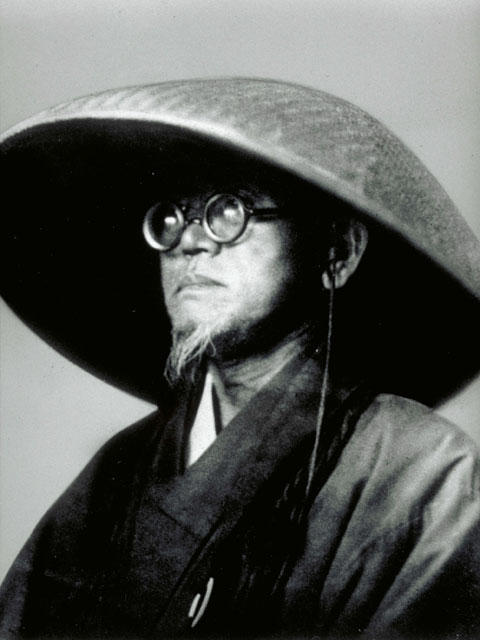
\includegraphics[width=\textwidth]{santoka}
\end{figure}

\chapter{\FK 献给祖父山头火}

{\FS

    \hfill 种田美奈子\footnotemark[1]

    \bigskip

    岁月流逝,在您逝世五十周年的时候,发生了一件难得而可喜的事情,这就是您的俳句被译成了中文。此刻我希望您的作品,能在同中国文化相结合的方面起到一定作用。

    回想起来,您走过了遥远的路程。一个人的足迹,竟然会同如此众多的人有着联系,您曾经这么问过自己吗?

    除了您走过的道路,没有能够找到维持生活的方法。您走过了自己认为无可奈何的道路。您得到了谅解您的人们的恩惠,才能够自始至终贯彻了创作自由律俳句\footnotemark[2]的意愿。这当然是您一生的憧憬。然而,您这样做,使我父亲陷入了孤独和苦恼的深渊\footnotemark[3]。说来,我已经到了时时感叹人生无常的年龄。我将凝眸等待您的作品的中文译本在中国出版,看它究意是什么样的面貌。最后,列出我所喜爱的您的俳句:

    \begin{quote}
        杜宇声声,明朝攀越彼山行。\\
        烈日炎炎,铁路笔直伸向前。
    \end{quote}

    \hfill 合掌

    \footnotetext[1]{\FS 本文作者是种田山头火的孙女,现住日本巧栖市。本文是她为日本版《山头火的世界·山头火秀句汉译集》撰写的前言。上梓前有所补充。本文为李芒译注。}
    \footnotetext[2]{\FS 传统俳句有五、七、五句式等格律,冲破格律,不拘音数句式等,即称自由律俳句。}
    \footnotetext[3]{\FS 山头火于一九二〇年、三十八岁时,与妻子协商离婚,由妻子扶养独生子健。尔后出家,继而开始托钵云游的生涯,并深入进句创作。因而,在生活上为亲友妻儿带来很多麻烦。}
}

\chapter{\FK 李芒先生为山头火增新辉}

{\FS

    \hfill 富永鸠山\footnotemark[1]

    \footnotetext[1]{\FS 本文作者是山头火研究会会长、著名书法家,本文是他为日本版《山头火的世界·山头火秀句汉译集》撰写的前言。本文为李芒译注。}

    \bigskip

    是俳句,还是痛苦\footnotemark[2],一开头,我就想这样写下去。山头火的生活道路和俳句创作,实际上都是在削割着自己的肉体,这也正是使得我非这样写下去不可的原因。

    \footnotetext[2]{\FS 俳句在日本也简称句(ku),ku和苦同音。}

    看上去,山头火象是在愚鲁中生活过来,也像随着罪孽的潮流漂泊不定。或者说,两者交错着,纠缠着,高迈和庸俗,美和丑,矜持和自嘲,安乐和悲哀,等等,只顾在思维和宿命的峡谷中,坚持不懈地摇橹行船。这样,山头火千真万确地生活了一个时代。他背负着一切,在创立一个世界,在自由律俳句创作方面,做出了历史上无与伦比的贡献。

    至今,关于山头火,发表过很多分析文章,应该说评价都是正确的。只是,我在同他唯一的儿子健先生一起旅行,询及山头火在味取观音堂的生活,然后又离开观音堂走上流浪行乞的旅途等经历,健先生只回答了一句话:「那是孤独的地狱。」这话在我听来最为鲜明,当时便反复想到到底是健先生直接同山头火接触过,话里充满真实的感情,而能打动听者的心弦。同时,也感觉到健先生自身的感情似乎是这样的。那么,在山头火心目中盘旋着的东西究竟是什么呢?也许连山头火本人也无法做出明确的回答,这只要看看山头火的生活、生平和俳句创作,也就会得到证明。

    山头火确实有着一种什么东西,能够使读者、研究者深思、沉醉和倾慕。观察一下他的句碑吧。山头火的句碑,当今在日本全国已建立了一百几十座。据说,要建的计划还很多,其中由个人建立的也达到相当的数目。这说明对山头火的倾慕达到了什么程度。

    铁钵会剧团上演的以山头火为主题的戏剧,把观众引进感动的热潮中去了。

    山头火的生平还被改编成电视剧和歌曲。真可以说,山头火已经使各个领域的人们感到了陶醉。

    一九八一年,山头火迎来了诞生一百周年纪念。当时,人们在收集资料的过程中,对山头火的评价分歧颇多。于是我想如若尽可能完整地把所有的山头火观收集起来,或许也是接近山头火的真实形象的一个手段。无论遭到怎样的歪曲,只要那形象活动在人们心目中,人们就会感受到一种真实,宝贵的真实,而这种真实又无疑是山头火所给与的影象。

    美国的乔·斯蒂文思先生出版了山头火的英译本,他通过对禅的研究发表了自己的研究论文和俳句的英译,为山头火文学增添了一个侧面,使人们看到更深一层的内含和扩展。

    我以书法为专业,是私塾的老师。因此,举行过三次日中友好书法展览。一九八五年,一个偶然的机会结识了当时在重庆市四川外语学院任教的宫本博子先生。她原是想把中国书法家介绍给我的。谈话中提到有位中国著名文学家正在研究山头火,收集资料,我就给这位先生寄去了一些。很快就收到回信,并附上墨书的山头火俳句和译文。汉字所固有的多样而深邃的表现力立刻就把我吸引住了。

    比如:
    \begin{quote}
        茕茕背影,缓步暮秋冷雨中。
    \end{quote}

    「茕茕」一词,辞典上说的是孤独无依,这种简洁而美妙的表现,赋与原作以生动的解释。

    这位译者就是中国社会科学院的李芒先生。我把自己受到的感动告诉了李芒先生,从此开始交往,曾经一度在东京做了彻夜长谈。山头火俳句集的中文译本在日本的出版,就这样迈开了第一步。

    这里,也出现了一位为山头火增新辉的人。

    于是,我们就是这样走近了山头火,山头火也展现出千姿百态。
    李芒先生不断地对译文进行推敲。他既注意到日中文化的差异,又苦心于确立自己的文学和山头火观。在中国,首次将日本的自由律俳句译成中文,这是一件需要决心和勇气的工作。

    中国,在翻译日本的定型俳句方面,已经在从事种种实验,还出现了「汉俳」这种形式,也就是说,用五、七、五句式把汉字排列在一起的形式。这种方法更接近俳句,正在得到普及。

    然而,现在是李芒先生向山头火的自由律俳句挑战,无疑这是具有历史意义的伟大挑战。看来,他的这种挑战已经在中国引起巨大的反响。大家知道,中国自古就有优秀的汉诗,它的形式已经在悠久的历史长河中固定下来。因此,如若没有相当的勇气和探索精神,是无法做到这一步的。我必须告诉读者,李芒先生倾注在山头火俳句翻译工作中的热情,是令人惊叹的!

    山头火俳句集日本版的出版,已经得到拥有版权的山头火家的慨允,也得到春阳堂出版社的支持。

    中国驻日大使馆一等秘书张光佩女士给以细致周到的指导和支持,也使我深受鼓舞,谨致衷心谢忱。

    另外,我最好的朋友肖宏先生始终同我合作,给予协助,亦借此机会致谢。

    山口县立图书馆的上野美代子女士、远藤制版绘图研究所的远藤夫妇、宇部高等学校的鹤田哲人先生以及防府彩色图片社的河合祥一先生等都给予大力支持,亦应致谢。

    这里,刊载了日本和中国书法家的作品,中国的有中国书法家协会理事费新我先生、北京篆刻家郑怀宝先生,日本的有书宗院院长、东宫书法进讲桑原翠邦先生等杰作,满足了我们和李芒先生的共同希望,使我们感到分外的光荣。

    最后,还要提出的是春阳堂书店和田欣之介社长、责任编辑永安浩美先生均曾给以无微不至的关怀。

    恰好在纪念山头火逝世五十周年的时候,我们遇到了这么多好人,得以使本书问世,确实是令人感激不尽的。

    在执笔撰写本文的过程中,有一种感想突然涌现在心头……

    这就是在这个不毛而又悖理的时代,要想跟山头火打交道,确实要怀有一颗求道而蕴含哲理的心。否则,是无法接近山头火的。

    这个山头火俳句的中文译本,如若能够加深日中两国的理解,有助于友好的文化交流,实为至幸。

    期待着李芒先生更加活跃。

    \bigskip

    \hfill 合掌
}

\chapter{\FK 喜读山头火佳句并赋汉俳六首}

{\FS \hfill 邹荻帆

    \begin{quote}
        岁暮读佳诗\\
        废寝忘餐人笑痴\\
        喜摘梅一枝

        细玩奇世珍\\
        一章一句一乾坤\\
        译作两传神

        斗笠落蜻蜓\\
        千秋独吟一俳人\\
        余晖青山青

        托钵寻诗行\\
        流水落花皆文章\\
        自有春芬芳

        蟋蟀曾伴眠\\
        俳人诗思能感天\\
        乡梦配管弦

        武士跛脚归\\
        曷若华章白鸽飞\\
        海外留心碑
    \end{quote}
}

\chapter{\FK 一个人的世界}

{\FS \hfill 李瑛

    种田山头火,这是一个陌生的日本诗人的名字,也正由于对这一陌生诗人的发现,使我们又得以认识了一个新的世界而感到兴奋和喜悦。

    世界,历史,人生和艺术,是多么真实而复杂的存在。属于它们的种种现象和生活在其中的人们的思想行为、甚或某些际遇,是美学家、哲学家研究探索的课题。

    山头火是这样一个人:他出生在日本大地主家庭,上过大学文学系,经过商,但辗转求业总不能持久,离婚后嗜酒参禅,曾因痛苦而自杀未遂,后被一和尚收留看守寺院,又因难以孤处,便一钵一笠漂泊乞讨。就这样,他走过了自己艰苦曲折的一生。在他所处的广阔背景下,他心灵深处的种种复杂思绪:欢乐,痛苦,感触和顿悟,凝成了数万首极富特色、独具个性的俳句,这是他人生阅历与体验的结晶,是他心灵自白的长卷。他在人生旅途的求索中,不断地发现着自己,寻找着自己,而我们则通过他的作品认识了一个人的世界。

    如今,他留下的这些俳句,同日本八世纪编成的古典诗歌总集二十卷的《万叶集》及其以后众多的日本和歌、俳句诗人所创作的卷帙浩繁的作品一样,巳成为日本人民诗歌宝库中重要的组成部分,受到人民的称誉,并越过大洋,在国外产生了很大影响。

    日本文学与中国文学有着源远流长的关系,特别是古典诗歌,尽管由于两国诗人所生活的地理、历史、政治、社会、思想、文化等多方面的原因,使之在思想倾向、人生态度和艺术见解等方面不尽一致,但却也有许多共同的方面,他们都在各自的限制中寻找充分袒露自己内心世界的自由。

    日本自《万叶集》问世以来,和歌在内容上,多为宫廷官吏和上层僧侣等应制与即兴咏怀之作,和人民现实生活距离较远,所咏对象也多是山川草木、自然景色,常常是触景生情,借以抒怀;虽然也有些表现个人贫困和民间习俗、民族风情的作品,但其接触领域和感情范围也不以广阔为尚;艺术上,则在传统规律的严格限制中,力求韵味含蓄、风格淡雅,由于篇幅短小,所以对语言文字的精练简约,要求很高。一般说来,从短歌派生出来的俳谐及其起句的独立形式俳句,除了将和歌这种崇尚高雅的艺术转到庶民手中,并增加了诙谐成分以外,基本上也是如此。而山头火的诗作,却打破了传统俳句定型格律的某些约束,追求自然淳朴,并强化语言的选择。他常常努力使作品负载更大的容量和产生高度的艺术表现力。通过自己的真挚感受,采取以小见大的手法,或隐喻,或暗示,使作品蕴含着深邃动人的感情。由于他不凡的经历,特别在他漂泊乞讨的生活中,行经各处,自然界的山山水水和各种物象,自然便成为他观察思考和表现的对象,他眼里的大自然也就全然不同于任何别人眼里的大自然。他通过自己饱尝人间酸甜苦辣和历经动荡之苦的观察感受,追求着一种意蕴和兴寄,借以抒发自己的情怀。

    在他一九二六年开始浪迹四方的乞讨生活之后几年,曾经历了十年侵略战争的年代,直到他一九四〇年去世。他既不从事物质生产,也不参加侵略战争,他既不笃信佛教的生死轮回,也不愿接近唯物的马克思主义;作为一个贫苦行僧,他只怀着满腔天真淳朴的感情,希望人与人不要互相残杀,而对人间疾苦、战乱死伤则表现了深挚的同情,任何人也不能不受历史的局限和制约。山头火就是这样一个人。译者李芒先生对他做了准确的研究和分析。是的,他就是这样一个人,一个具体存在的人,一个企望遁世却又不能与世隔绝的人,一个活生生的单纯而又复杂的人,他只相信「我在创造」,他是怀着一片诚挚的心「作我独自的真诚的诗」的。

    在他所经历的复杂感情与体验中,不少诗表现了他对勃勃生机的大自然的执着和由衷的爱。

    \begin{quote}
        几番晴日几番雨,稻苗青满畦。\\
        烟霞袅袅重重山,山是我家园。
    \end{quote}

    这里,通过稻田中满眼青青的禾苗和重峦间缭绕的烟霞,表现出作者何等强烈的对生活的赞美和眷恋情怀!有些还明显的融进了他睿智的哲学思考。

    在他放浪四方的空茫与孤寂中,在他低沉痛苦的行脚生涯中,自然会时时怀念离去的故里:

    \begin{quote}
        故乡归路遐,春树绽新芽。\\
        涛声只不断,故里巳遥远。\\
        皓月频招唤,故乡节庆酣。
    \end{quote}

    仿佛是一步一回首的深沉思念,联及此时此刻,此情此景,仔细玩味,字里行间渗透出浓重的难以名状的隐衷和复杂的感情。

    尽管他内心和境遇苦难重重,却始终未因困厄而绝望,他的不少诗虽难免染就孤凄悲凉的色调和一种虚幻的宗教感情,但更为深沉的是,从他的诗句中,传达出他对人世深层的慨叹和感喟,对人生忧患的某种彻悟,并且仍能从中发掘出美来。一只蜻蜓,一匹蟋蟀,远山近水,春花秋树,头上的云霞冷雨,脚下的碧草青禾,甚至屋檐融雪的滴水声,都蕴含着他无限真挚的思绪,成为一种美,一种宁静高洁的美、一种纯净的尊严美、一种能够撼动人们心灵的力量。

    说来奇怪,我在每每阅读日本短歌、俳句时,总觉得许多日本诗人都很善于运用绘画中的「留白」技法,使之以无胜有,以虚寓实。在作品中,虽然只作极少的细致的点染,而留出极富魅力的「艺术空白」,成为读者驰骋想象的天地,极大地丰富和补充了作品的意境和气氛,从而产生深长的韵味和强烈的艺术效果。

    \begin{quote}
        月色清明舟自横,且睡其中。
    \end{quote}

    这里山头火只写了月色皎洁,无以为家,在一只小舟中睡去,而读者读后得到的,除此之外,却兴起了更多的联想,诸如:一天长途跋涉行乞的劳顿,长空下月光照着寂寥的旷野、荒僻的河畔,也许是行经野渡,发现一只无人小舟,便进去睡了的野趣;在这里,读者不仅可以想象出作者此时的心境和神态,还仿佛可以看见河中的月光倒影,听见四野的虫鸣、水声,甚至可以闻见岸边潮湿里野艾蔓草的浓重气息……这种读者感觉中联想的景物的美,比起直观表达的景物的美,似乎更丰富,更强烈,更含蓄,因而也更耐人寻味。这种精心处理的「艺术空白」,大大拓展了人们的想象力,直接丰富了人们生命的容量,从而有助于人们的感情陶冶和心灵建设。

    作为一个特定时代的日本诗人的心灵经历,山头火对于我们确实是一片深沉广阔的大陆,一个奇异的世界。我想,中国读者对于他所袒露的自己不同寻常的真诚和单纯的心史,会是完全可以理解并热爱的。

    俳句在日本人民中间有广泛的群众基础,深受日本人民的喜爱。据说在日本,专业和业余的俳句作者至少有三百多万;他们有专门研究讨论俳句创作和活动的组织,有专门编辑出版俳句的刊物。俳句这种体制短小、极富民族特色的诗歌形式的创作,在日本正在得到日益繁荣和发展,在国外也正在产生越来越大的影响。

    李芒先生华生致力于日本文学研究和译著,是我国文学界十分熟悉的著名学者和翻译家。他不仅熟谙日本文学,而且对中国文学特别古典诗词也有很深的造诣。他译著颇丰,只就和歌和俳句的汉译问题,就曾写过多篇学术长文,引起国内和日本学者、专家的兴趣和重视。现在,又为我们介绍了一位早应结识的俳句诗人。俳句比起日本现代诗和短歌来,因其体制更短,语言的回旋余地更小,而各国文字又各有不同的规律和特点,所以翻译的难度更大,要求更高;李芒先生以其严肃认真的态度,力求最大限度地把原作的神韵和境界准确地表现出来,他对原作者的深刻研究和对译作的反复推敲,精益求精的严谨治学精神,是使人钦佩的。如今,他把鲜为我国读者所知的山头火的俳句在纪念诗人逝世五十周年的今天第一次介绍给我们,不仅有助于我们欣赏和借鉴他的诗作,进一步认识日本文学和日本诗歌的发展,也为增强中日两国文化交流、促进两国人民和诗人之间的友谊和了解作出了新的贡献,为此,我们应该衷心地感谢他。

    \bigskip

    \hfill 一九八九年二月十六日于北京
}

\chapter{\FK 山头火与自由律俳句}
{\FS

    \hfill 刘德有

    \bigskip

    在中国,把种田山头火这位日本俳人和他的俳句介绍给读者的,大概要算李芒同志是第一位了。我在《日语学习与研究》杂志(一九八六年第六期)上看到李芒同志发表的《论山头火并佳句选译》时,真有一种难以言状的喜悦。我佩服他的眼力,他的学识,他的胆量,更为他那一颗火一样的探求心所感动。

    李芒同志的论文,使我想起了一件事。那是一九八六年十一月,日本著名剧作家宫田三先生来北京,我们见面时他送我一本书,名叫《{\FM うしろ姿のしぐれていくか}》(茕然背影,缓步暮秋冷雨中\footnotemark[1])。翻开阅读,方知是一部剧本,写的是一位漂泊行乞的俳人种田山头火。「{\FM うしろ姿のしぐれていくか}」,既是剧名,也是这位俳人的代表作。

    \footnotetext[1]{\FS 本人引用的山头火俳句的译文,除注明者外,均出自李芒同志之手。}

    山头火这个名字,当时对于我是陌生的。不消说,他的俳句我也是第一次接触。读了山头火的俳句,使我感到新鲜、活泼、开阔、舒展,就像一个长年屈居斗室的人,突然看见了碧蓝的大海。

    俳句是日本韵文学的一种传统形式,也是世界上最短的格律诗。但,山头火向传统挑战,冲破格律,创作了上万首「自由律俳句」。他不受三节十七字(五、七、五)的束缚,他无视季题,也很少使用「切れ字」(断句的助词或助动词)。我们知道,在俳句史上,确有一些名家偶然也违背俳句禁律写一些灵动有致的句作。同时我们也知道,写「自由律俳句」也并非自山头火始。但应该说,山头火是向俳句传统进行挑战最为彻底的一个。

    诗,应该迸发生命的火花,发露诗人的情感。俳句也不例外。俳句要在被规定了音数的短句中表现诗人的世界。但是,仅仅音数齐整,做到了五、七、五,也未必就是俳句。例如「{\FM とびだすな車は急に止まれない}」,就不是俳句,而只是一条宣传交通规则的标语而巳。其次,即使合乎格律,音数齐整,含有季题,也未必就是一首好俳句。因为它虽然有外在的韵律美,但如果是「无病呻吟」,没有唱出作者的心声,就不是诗,因而就不能打动人。

    而山头火呢?他的俳句虽然不注重外在的韵律美,但它们着意奇拔,句句闪动着作者的灵感,句句具有神韵,句句是诗,因而不能不感人,不能不引起强烈共鸣。请看他的几首俳句。
    \begin{quote}
        {\FM 分け入つても分け入つても青い山}\\
        (拨草行行复行行,此身犹在青山中。)

        {\FM 朝の橋をわたるより乞いはじめる}\\
        (清晨过此桥,开始行乞讨。)

        {\FM 鉄鉢の中へも霰}\\
        (铁钵铮铮鸣,亦闻落霰声。)

        {\FM だまつて今日の草鞋穿く}\\
        (默默无言,且将今日草鞋穿。)

        {\FM こころわびしくひとりまた火を焚く}\\
        (胸怀寂然,独自又将炊火燃。)

        {\FM 笠にとんぼをとまらせてあるく}\\
        (且凭斗笠落蜻蜓,伴吾一路行。)

        {\FM 咳がやまない背中をたたく手がない}\\
        (连连咳嗽,却无为我捶背手。)

        {\FM 酔うてこほろぎと寝ていたよ}\\
        (陶然吃酒醉,蟋蟀曾同睡。)

        {\FM 寝ころべば枯草の春匂ふ}\\
        (躺一躺,但闻枯草散春芳。)
    \end{quote}

    山头火正是通过这些「自由律」俳句迸发出他的生命火花,表达了他的强烈情感。

    我这样说,丝毫也没有要贬低传统俳句的意思,相反地,我酷爱传统俳句。那些优美典雅,或风格清新,或情景交融,或触思抒怀的传统俳句,我认为只要它们是真正的诗,就具有艺术的魅力,就会感染读者,就能拨动人们的心弦。迄今为止,日本留下了那么多脍炙人口的传世名句,便是明证。然而,在山头火来说,他如果墨守格律,不采取自由律,也许是写不出那样生动活泼、清新泼辣的惊人之句的。山头火之所以要打破格律束缚,去追求自由律,我以为恐怕跟他的身世、经历、思想和艺术观有密不可分的关系。

    山头火(一八八二—一九四〇)是山口县防府市人,十一岁时母亲跳井自杀,使他精神上受到很大打击。他在早稻田大学文学系二年级就学时因患神经衰弱症中途退学返乡,跟父亲共同开办酿酒厂而宣告破产。后迁居熊本,三十九岁时与妻子离婚,并转赴东京谋生,但未获成功。他痛苦失望,生活放荡,进一步嗜酒,后返回熊本当了和尚,开始了「一钵千家饭」的行脚讨乞生涯。山头火生活的年代正是日本资本主义兴起发展,对外频频发动战争,国内各种矛盾日益激化的年代。这些都决定了他复杂的世界观:他叹息人生无常,感到寂寥、孤寒,但他热爱生活,热爱大自然;他是一个不折不扣的人道主义者,他不希望人与人互相残杀,但无法洞察战争的本质。激烈动荡的社会,无情地拨弄着他的命运,但他一心希望能成为一个诚实的人,努力进行他的俳句创作。山头火写道:「天不灭我,叫我作诗;我活着作诗,作我独自的真诚的诗。」我们可以说,恰恰是山头火的生活内容,决定了他采用自由律的形式写俳句;而自由律俳句又最好地最生动地表现了他的生活、他的思想和情感。

    也许有人会说,「写自由律俳句,不是无异于写短句的自由诗吗?」「格律和季语是俳句的生命,否定了它们,不就是否定俳句本身吗?」「既要写俳句,又要打破格律,山头火不是自相矛盾吗?」是的,山头火选择的,正是一条矛盾的路。诚然,他冲破了俳句的格律,但他没有放弃俳句。他在坚持俳句的过程中,去反抗被视为俳句生命的各种格律的束缚,给俳句注入了新的生命。艺术从来贵在创新,艺术要求个性。从这个意义上说,山头火的俳句打破格律,完全符合艺术的规律,它本身就是艺术,或者说它反映了山头火的艺术观。

    我们知道,传统俳句有季语,是日本风土培育出来的日本人的美意识的反映,它同日本美丽的大自然和四季的更换以及生活在这一自然环境中的日本人的异常细腻而反应十分灵敏的情感、心态等有着密不可分的关系。山头火同样也生活在这样的大自然和环境之中。他虽然不受季语的束缚,但也不是绝对不使用季语。上述「{\FM うしろ姿のしぐれていくか}」「{\FM 鉄鉢の中へも霰}」句中的「{\FM しぐれ}」、「{\FM 霰}」就是季语。但山头火不是把它们作为季语,而是作为映入他眼中的自然景物写进了俳句之中。这就是说,山头火尽管反对格律,不受季语束缚,不去有意识地歌唱季节,但他也终于不能摆脱季节,不能脱离开俳句本身。

    按习惯,日本的短歌和俳句常常在句前加题,或附以小序,以便有助于读者加深对这些短歌或俳句的理解,而不使人们感到唐突。但山头火的俳句却极少加题或附以小序。即使这样,也不使人感到唐突而能够很好地理解它,这是因为读他的俳句的人一般都了解他的生活经历的缘故。从某种意义上说,山头火的生活和他的云游本身就是他的俳句的序。而这同时也是他的自由律得以成立的最大因素。山头火的自由律俳句,乍一看似乎是随便写写,不经推敲,写完了事。但实际上,他无论走到哪里,总是带着笔记本和一支钢笔,不知疲倦地写,不断地修改,不断地推敲。由此可见,他的创作态度是严肃的。

    \begin{quote}
        {\FM 雨ふるふるさとははだしであるく}\\
        (故乡冷雨中,托钵归来赤脚行。)
    \end{quote}

    读了这首俳句,无需多加说明,在我们眼前浮现的是这样一幅景象:头戴斗笠,手持铁钵,身披黑袍的山头火来到山口县旧居门前。如今他巳成为行乞的僧人,他不愿被熟人认出他来,便故意把斗笠戴得很深,在雨中赤脚匆匆走过。

    还有,据说山头火在旅行时腰间总是缠着一个包裹,里面包的是自杀了的母亲的牌位。他一生中写了许多怀念母亲的俳句,可见他对母亲有着深厚的感情。他在母亲忌日那一天,创作了这样的俳句:

    \begin{quote}
        {\FM うどん供えて、母よ、わたくしもいただきまする}\\
        (面条供灵前,母亲哟,儿与您老同吃面。\footnotemark[1])
    \end{quote}

    \footnotetext[1]{\FS 此句为笔者所译。}

    山头火的诗句虽没有气魄宏大、苍茫深沉的风格,但有寄托感慨、意境深远的铺述手法。他的俳句,语言简明平易,但表现出深邃的内涵,具有艺术的魅力和美学价值。

    山头火在运用语言和造句方面,确实是独具匠心的。在日语中,五音和七音的句子读起来,琅琅上口,节奏感很强。这是「五、七、五、七、七」的短歌和「五、七、五」的俳句得以广泛流传的重要条件。为什么山头火的那些打破这一格律的自由律俳句也能使人读起来感到优美和谐、铿锵有力呢?我想,这是因为山头火虽然写的是不规则句子,但仍注意节奏感的缘故,例如「{\FM うしろ姿のしぐれていくか}」(音数为两节,七、七音),「{\FM 月がまねくふるさとはおまつり}」(三节,六、五、四),「{\FM 炎天をいただいて乞い歩く}」(三节,五、五、五),「{\FM 水のうまさを蛙鳴く}」(二节,七、五),「{\FM わがままきままな旅の雨にぬれてゆく}」(三节,八、六、五),「{\FM 落葉しつくしたる木の実の赤く}」(二节,九、六)。从以上的分析来看,这些句子中有许多五音和七音。这一现象是饶有兴趣的。这也表明山头火自由律俳句的语言,通过运用节奏感很强的五、七音加强了艺术效果。

    俳句,从它的发生和发展来看,走过了不断革新的道路。我们完全有理由说,随着时代的变迁,那种严守格律的传统俳句,今后也将在不断创新中继续发展。而自由律俳句,作为俳句发展中的一个流派,自有它产生的客观条件。自由律俳句的兴起,使传统俳句也吸收了有生命力的因素。而山身火对传统的反抗和挑战,实际上在客观上也起了使传统俳句以某种形式得到加强的作用。这大概就是事物的辨证法吧。

    山头火,是他的家乡山口县防府市的骄傲。

    最近,听说山口县防府市要把李芒同志的论文连同他翻译的山头火的俳句汇编成册,付梓出版,这是令人十分高兴的事。我对此表示衷心祝贺。我认为该书的出版一定能在中日两国人民、两国文学家的心灵与心灵中间架起一座友谊和相互了解的桥梁。

    李芒同志是我的挚友,我与他最早相识,是一九六一年春在东京举行亚非作家紧急会议时。那时我们作为代表团的成员第一次合作,他给我留下了深刻的印象。李芒同志为人诚挚、谦和、热情、朴实,具有长者风度。他知识渊博,特别是对日本文学有很深的造诣。当我知道他在中专读了一年书后便参加工作,年轻时做过火车司炉,而他的渊博的学识和高水平的日语是后来全靠自学掌握的时候,更加钦佩和尊敬他。

    李芒同志曾翻译过许多日本小说,也写过不少关于日本文学的评介。最近几年,他花费大量的精力和时间翻译介绍和歌、俳句。他在和歌与俳句的翻译实践方面有很多大胆的尝试和创新,丰富了我国翻译日本韵文的实践。不仅如此,更加可贵的是,李芒同志把他在翻译和歌俳句方面获得的经验上升为理论,提出了一些重要的独到的见解。我们知道,韵文的翻译是极为困难的。翻译和歌、俳句也是如此。李芒同志主张译者要「深入体会原诗的思想感情和艺术特点,与诗人打成一片」。他认为,原作与译文「都是『创作』,但却是两种不同的创作」。译者在把诗人的艺术品译成另外一种文字时,要「在力争将原作的内容与形式最大限度忠实地翻译出来方面进行创作,并努力使译文成为基本上与原作相同的艺术品。」他认为,「短歌和俳句内容各异,形式不一,从而译文也应主要从内容出发,注重神韵、风格和节奏的表现,兼顾形式的其他方面。」「总的精神是在釆取灵活多样的形式和方法的基础上,逐步增多地釆取适当的定型化的译法。」他主张,在「语言方面,一方面采取古典诗歌的格调,尽可能照顾到平仄规律」,「实在译不成者也在适当照顾到平仄规律的前提下译成古诗、长短句等。一方面既釆取古典诗歌的形式,又照顾到便于今人阅读,适当采用较之原歌原句稍微平易的词语,避免过分古雅难懂。」我认为,这些意见都是颇值得倾听的。李芒同志这次翻译山头火的自由律俳句,就采取了古诗的格律,尽量使用平易语言,即口语古调的方法。正是李芒同志基于这一原则的辛勤劳动,今天使更多的中国读者和日本文学爱好者读到了山头火的作品。

    当然,翻译和歌、俳句,完全可以有各种不同的方法。有关日本传统韵文的翻译理论研究尚待进一步深化,同时理论创造也允许有不同的见解和主张。我们在科学和学术领域里实行「百家争鸣」,无疑有利于促进我国的科学学术事业的不断发展。我期望在和歌、俳句的汉译方面能出现一个互相展开意译、「百花齐放」,「百家争鸣」的繁荣局面。

    李芒同志作为日本文学研究会副会长、中国外国文学学会常任理事、中国翻译工作者协会理事,为译介日本文学作品已经作出了很大贡献。希望他今后继续奋起健笔,在这一方面取得更丰硕的成果。我想,这绝不只是我一个人的愿望吧。

    作为一个日本文学爱好者的后辈,我不揣冒昧写了这一些不成熟的想法,是为序。
}

\chapter{\FK 本文}
\setcounter{haikucounter}{0}

\begin{haiku}
    {\FH 松風に明け暮れの鐘\ruby[g]{撞}{つ}いて。}

    {\FK 飒飒松风,撞罢晨钟又暮钟。}
\end{haiku}

\begin{haiku}
    {\FH ひさしぶりに掃く\ruby[g]{垣根}{かきね}の花が咲いてゐる。}

    {\FK 久疏持帚来,欲扫篱笆花正开。}
\end{haiku}

\begin{haiku}
    {\FH 分け入つても分け入つても青い山。}

    {\FK 拨草行行复行行,此身犹在青山中。}

    {\FS 此句前言为「大正十五年(一九二六)四月,背负着无法解决的迷惑、走上行乞流浪的旅途」,表现了找不到出路的情绪。}
\end{haiku}

\begin{haiku}
    {\FH しとどに濡れてこれは道しるべの石。}

    {\FK 雨淋精湿,却是一枚指路石。}
\end{haiku}

\begin{haiku}
    {\FH 炎天をいただいて\ruby[g]{乞}{こ}ひ歩く。}

    {\FK 头顶烈炎天,化缘走向前。}
\end{haiku}

\begin{haiku}
    {\FH 鴉啼いてわたしも一人。}

    {\FK 孤鸦一声鸣,吾亦一人行。}
\end{haiku}

\begin{haiku}
    {\FH 生死の中の雪ふりしきる。}

    {\FK 生死轮回中,霏霏白雪积重重。}

    {\FS 此句前言为「认清生死乃佛家一大事之因缘也」。}
\end{haiku}

\begin{haiku}
    {\FH 木の葉散る歩きつめる。}

    {\FK 树叶正飘零,云游步不停。}
\end{haiku}

\begin{haiku}
    {\FH 張りかへた\ruby[g]{障子}{しょうじ}のなかの一人。}

    {\FK 格子拉门新糊过,室中只我一人坐。}
\end{haiku}

\begin{haiku}
    {\FH 踏みわける萩よすすきよ。}

    {\FK 芒草胡枝子,拨开踏倒步迟迟。}

    {\FS 此句前言为「昭和二、三年(一九二七、八),毫无目标地徘徊在山阳道、山阴道和四国九州一带」。}
\end{haiku}

\begin{haiku}
    {\FH この旅、果もない旅のつくつくぼうし。}

    {\FK 此次云游,寒蝉孤飞无尽头。}
\end{haiku}

\begin{haiku}
    {\FH へうへうとして水を\ruby[g]{味}{あじわ}ふ。}

    {\FK 悠然独享,且将清水味道尝。}
\end{haiku}

\begin{haiku}
    {\FH 落ちかかる月を観てゐるに一人。}

    {\FK 月亮正西沉,遥望只一人。}
\end{haiku}

\begin{haiku}
    {\FH \ruby[g]{投}{な}げだしてまだ陽のある脚。}

    {\FK 坐地伸双腿,脚上悠然尚落晖。}
\end{haiku}

\begin{haiku}
    {\FH 山の奥から繭負うて来た。}

    {\FK 人自深山外,遥遥负茧来。}
\end{haiku}

\begin{haiku}
    {\FH 笠にとんぼをとまらせてあるく。}

    {\FK 且凭斗笠落蜻蜓,伴吾一路行。}
\end{haiku}

\begin{haiku}
    {\FH 歩きつづける彼岸花咲きつづける。}

    {\FK 行走不停步,曼珠沙华开一路。}

    {\FS「曼珠沙华」据说原意为红色,日本称彼岸花、天涯花、死人花、幽灵花、舍子花等。曼珠沙华是日本的梵文译音。它有毒而多生于墓地,一般认为是不吉利的花,然而秋季一枝能开多朵嫣红的花,很美。中国称石蒜、龙爪花、蟑螂花等。}
\end{haiku}

\begin{haiku}
    {\FH まつすぐな道でさみしい。}

    {\FK 只有笔直路一条,行来更寂寥。}
\end{haiku}

\begin{haiku}
    {\FH だまつて今日の草鞋\ruby[g]{穿}{は}く。}

    {\FK 默默无言,且将今日草鞋穿。}
\end{haiku}

\begin{haiku}
    {\FH ほろほろ酔うて木の葉ふる。}

    {\FK 树叶落翩翩,犹如酒醉飘飘然。}
\end{haiku}

\begin{haiku}
    {\FH しぐるるや死なないでゐる。}

    {\FK 冬初雨凄凄,人犹未死去。}
\end{haiku}

\begin{haiku}
    {\FH 水に影ある旅人である。}

    {\FK 水中投影有吾身,吾本一旅人。}
\end{haiku}

\begin{haiku}
    {\FH しぐるるやしぐるる山へ歩み入る。}

    {\FK 冬初雨凄凄,雨中走进深山去。}
\end{haiku}

\begin{haiku}
    {\FH 生き残つたからだ\ruby[g]{掻}{か}いてゐる。}

    {\FK 此身得以活下来,搔痒怡心怀。}
\end{haiku}

\begin{haiku}
    {\FH また見ることもない山が遠ざかる。}

    {\FK 相识无缘又一山,离吾渐渐远。}
\end{haiku}

\begin{haiku}
    {\FH どうしようもないわたしが歩いてゐる。}

    {\FK 心怀无可奈何情,独自向前行。}
\end{haiku}

\begin{haiku}
    {\FH 分け入れば水音。}

    {\FK 拨草走进深山中,且闻流水声。}
\end{haiku}

\begin{haiku}
    {\FH すべつてころんで山がひつそり。}

    {\FK 滑倒又跌倒,山岭静悄悄。}
\end{haiku}

\begin{haiku}
    {\FH すつかり枯れて豆となつてゐる。}

    {\FK 枝叶尽干枯,却有豆成熟。}
\end{haiku}

\begin{haiku}
    {\FH 捨てきれない荷物のおもさまへうしろ。}

    {\FK 家什不肯丢,沉重背前后。}
\end{haiku}

\begin{haiku}
    {\FH あの雲がおとした雨にぬれてゐる。}

    {\FK 我身淋湿雨纷纷,降自中天那片云。}
\end{haiku}

\begin{haiku}
    {\FH 年とれば故郷こひしいつくつくぼうし。}

    {\FK 人到老年,萦怀故里一秋蝉。}
\end{haiku}

\begin{haiku}
    {\FH 水音といつしよに里へ下りて来た。}

    {\FK 水声作伴,下山来到小村前。}
\end{haiku}

\begin{haiku}
    {\FH まつたく雲がない笠をぬぎ。}

    {\FK 长空闲静无云翼,摘下斗笠。}
\end{haiku}

\begin{haiku}
    {\FH 墓がならんでそこまで波がおしよせて。}

    {\FK 坟墓并排一座座,涌向前来有海波。}
\end{haiku}

\begin{haiku}
    {\FH 酔うてこほろぎと寝てゐたよ。}

    {\FK 陶然吃酒醉,蟋蟀曾同睡。}
\end{haiku}

\begin{haiku}
    {\FH 雨だれの音も年とつた。}

    {\FK 茅檐滴雨声,竟亦临衰境。}
\end{haiku}

\begin{haiku}
    {\FH 物乞ふ家もなくなり山には雲。}

    {\FK 再乞食巳无人家,且眺望山上云霞。}
\end{haiku}

\begin{haiku}
    {\FH 笠も\ruby[g]{漏}{も}りだしたか。}

    {\FK 侬一斗笠,亦漏潇潇雨。}
\end{haiku}

\begin{haiku}
    {\FH 霜夜の\ruby[g]{寝床}{ねどこ}がどこかにあらう。}

    {\FK 霜夜沉沉,总有一处可安身。}
\end{haiku}

\begin{haiku}
    {\FH うしろすがたのしぐれてゆくか。}

    {\FK 茕然背影,缓步暮秋冷雨中。}

    {\FS 此句标题为「自嘲」,并有前言说:昭和六年(一九三一),本想在熊本市落脚,但终未成功,只好继续云游四方,别无良策。}
\end{haiku}

\begin{haiku}
    {\FH \ruby[g]{鉄鉢}{てつぱつ}の中へも霰。}

    {\FK 铁钵铮铮鸣,亦闻落霰声。}
\end{haiku}

\begin{haiku}
    {\FH ふるさとは遠くして木の芽。}

    {\FK 故乡归路遐,春树绽新芽。}
\end{haiku}

\begin{haiku}
    {\FH 笠へぽつとり椿だつた。}

    {\FK 忽闻斗笠响一声,却是山茶正落英。}
\end{haiku}

\begin{haiku}
    {\FH 今日の道のたんぽぽ咲いた。}

    {\FK 今日行小径,着花喜见蒲公英。}
\end{haiku}

\begin{haiku}
    {\FH 雨ふるふるさとははだしであるく。}

    {\FK 故乡冷雨中,托钵归来赤脚行。}
\end{haiku}

\begin{haiku}
    {\FH うつりきてお彼岸花の花ざかり。}

    {\FK 方始迁来,曼珠沙华正盛开。}
\end{haiku}

\begin{haiku}
    {\FH 草の\ruby[g]{実}{さね}の露のおちつかうとする。}

    {\FK 草籽宿露珠,似欲且长住。}
\end{haiku}

\begin{haiku}
    {\FH ゆふ空から柚子の一つをもらふ。}

    {\FK 遥对晚霞如锦绣,且来索取一颗柚。}
\end{haiku}

\begin{haiku}
    {\FH 月が昇つて何を待つでもなく。}

    {\FK 皓月东升入碧穹,并非怀有待何情。}
\end{haiku}

\begin{haiku}
    {\FH ひとりの火の燃えさかりゆくを。}

    {\FK 独将炊火燃,愈旺愈开颜。}
\end{haiku}

\begin{haiku}
    {\FH 誰か来さうな空が曇つてゐる枇杷の花。}

    {\FK 似有谁人来我家,阴天喜绽枇杷花。}
\end{haiku}

\begin{haiku}
    {\FH 音は朝から木の実をたべに来た鳥か。}

    {\FK 何物枝头闹?必是啄食树籽声,小鸟飞来早。}
\end{haiku}

\begin{haiku}
    {\FH ぬいてもぬいても草の\ruby[g]{執着}{しゅうじゃく}をぬく。}

    {\FK 拔来又拔去,拔不尽青草执着意。}
\end{haiku}

\begin{haiku}
    {\FH もう明けさうな窓あけて青葉。}

    {\FK 似近黎明,推窗唯见叶青青。}
\end{haiku}

\begin{haiku}
    {\FH すつばだかへとんぼとまらうとするか。}

    {\FK 试问蜻蜓,欲在赤光身上停?}
\end{haiku}

\begin{haiku}
    {\FH かさりこそり音させて鳴かぬ虫が来た。}

    {\FK 窸窸窣窣发轻声,虫豸爬来却不鸣。}
\end{haiku}

\begin{haiku}
    {\FH 花いばら、ここの土とならうよ。}

    {\FK 野薇开簇簇,吾身欲作此处土。}
\end{haiku}

\begin{haiku}
    {\FH 山のいちにち蟻もあるいてゐる。}

    {\FK 一日山中方独步,却知蚂蚁犹行路。}
\end{haiku}

\begin{haiku}
    {\FH 雲がいそいでよい月にする。}

    {\FK 只为月亮更清丽,白云迅飞去。}
\end{haiku}

\begin{haiku}
    {\FH けふはおわかれの\ruby[g]{糸瓜}{へちま}がぶらり。}

    {\FK 今日将分手,丝瓜亦垂头。}
\end{haiku}

\begin{haiku}
    {\FH かすんでかさなつて山がふるさと。}

    {\FK 烟霞缥渺重重山,山是我家园。}
\end{haiku}

\begin{haiku}
    {\FH 春風の鉢の子一つ。}

    {\FK 春风和煦,铁钵伴我云游去。}
\end{haiku}

\begin{haiku}
    {\FH ひさびさもどれば\ruby[g]{筍}{たかんな}によきによき。}

    {\FK 久别归庵望,竹笋正呈祥。}
\end{haiku}

\begin{haiku}
    {\FH 家を持たない秋がふかうなるばかり。}

    {\FK 无家可归宿,唯有清秋暮。}
\end{haiku}

\begin{haiku}
    {\FH わがままきままな旅の雨にはぬれてゆく。}

    {\FK 咨情行旅处,一路雨淋湿漉漉。}
\end{haiku}

\begin{haiku}
    {\FH びつしょり濡れて代掻く馬は叱られてばかり。}

    {\FK 耙田耕马尽淋湿,却总受呵叱。}
\end{haiku}

\begin{haiku}
    {\FH はれたりふつたり青田になつた。}

    {\FK 几番晴日几番雨,稻苗青满畦。}
\end{haiku}

\begin{haiku}
    {\FH 草しげるそこは死人を焼くところ。}

    {\FK 碧草萋萋,此处原为火葬地。}
\end{haiku}

\begin{haiku}
    {\FH 炎天かくすところなく水のながれくる。}

    {\FK 炎天无处藏身影,清流却送水泠泠。}
\end{haiku}

\begin{haiku}
    {\FH 日ざかりのお地蔵さまの顔がにこにこ。}

    {\FK 阳光照耀,地藏菩萨面含笑。}
\end{haiku}

\begin{haiku}
    {\FH 待つでも待たぬでもない雑草の月あかり。}

    {\FK 似等非等自多情,杂草莹莹皓月明。}
\end{haiku}

\begin{haiku}
    {\FH 蚊帳へまともな月かげも誰か来さうな。}

    {\FK 蚊帐清明笼月影,似有谁来慰孤零。}
\end{haiku}

\begin{haiku}
    {\FH 散るは柿の葉咲くは茶の花ざかり。}

    {\FK 柿叶方凋残,茶花正竞妍。}
\end{haiku}

\begin{haiku}
    {\FH 空のふかさは落葉しづんでゐる水。}

    {\FK 欲度天空深几许,且观落叶沉水底。}
\end{haiku}

\begin{haiku}
    {\FH うしろから月のかげする水をわたる。}

    {\FK 月光来背后,踏影渡河流。}
\end{haiku}

\begin{haiku}
    {\FH とぼしいくらしの屋根の雪とけてしたたる。}

    {\FK 家贫屋顶雪莹莹,春日且闻滴水声。}
\end{haiku}

\begin{haiku}
    {\FH 焚くだけの枯木はひろへた山が晴れてゐる。}

    {\FK 拾得干柴足烧饭,晴光一片照山峦。}
\end{haiku}

\begin{haiku}
    {\FH よびかけられてふりかへつたが落葉林。}

    {\FK 忽闻呼唤方回首,却是林中落叶稠。}
\end{haiku}

\begin{haiku}
    {\FH 雪のあかるさが家いつぱいのしづけさ。}

    {\FK 瑞雪莹莹,室内清光一片静。}
\end{haiku}

\begin{haiku}
    {\FH ふくろうはふくろうでわたしはわたしでねむれない。}

    {\FK 我自幽居枭自鸣,长夜梦难成。}
\end{haiku}

\begin{haiku}
    {\FH けさは水音も、よいたよりでもありさうな。}

    {\FK 今朝水声亦含情,似有佳音慰茕茕。}
\end{haiku}

\begin{haiku}
    {\FH 生えて伸びて咲いてゐる幸福。}

    {\FK 发芽生长又开花,幸福应无涯。}
\end{haiku}

\begin{haiku}
    {\FH 閉めて一人の障子を虫が来てたたく。}

    {\FK 一人独处闭拉门,却闻虫豸叩频频。}
\end{haiku}

\begin{haiku}
    {\FH 山から山がのぞいて梅雨晴れ。}

    {\FK 此山望彼山,梅雨方停晴满天。}
\end{haiku}

\begin{haiku}
    {\FH 食べる物はあつて酔ふ物もあつて雑草の雨。}

    {\FK 有物可食有酒醉,杂草雨霏霏。}
\end{haiku}

\begin{haiku}
    {\FH いつでも死ねる草が咲いたり実つたり。}

    {\FK 草花开放又结实,观此随时均可死。}
\end{haiku}

\begin{haiku}
    {\FH 日ざかり落ちる葉のいちまい。}

    {\FK 烈日炎炎,落叶孑然只一片。}
\end{haiku}

\begin{haiku}
    {\FH ふるさとの水をのみ水をあび。}

    {\FK 故里水粼粼,润喉又洗身。}
\end{haiku}

\begin{haiku}
    {\FH お彼岸のお彼岸花をみほとけに。}

    {\FK 曼珠沙华春分摘,献与佛爷免祸灾。}
\end{haiku}

\begin{haiku}
    {\FH 彼岸花さくふるさとはお墓のあるばかり。}

    {\FK 曼珠沙华开簇簇,故乡处处皆坟墓。}
\end{haiku}

\begin{haiku}
    {\FH 重荷を負うてめくらである。}

    {\FK 背负重荷行,双目已失明。}
\end{haiku}

\begin{haiku}
    {\FH 月も水底に旅空がある。}

    {\FK 羁旅青空沉水底,且看皓月为佳侣。}
\end{haiku}

\begin{haiku}
    {\FH 昼寝さめてどちらを見ても山。}

    {\FK 午睡方睁眼,望去周遭尽是山。}
\end{haiku}

\begin{haiku}
    {\FH よい宿でどちらも山で前は酒屋で。}

    {\FK 好旅宿,四面青山对门是酒铺。}
\end{haiku}

\begin{haiku}
    {\FH ここで寝るとする草の実のこぼれる。}

    {\FK 草籽频频飞,便于此处睡。}
\end{haiku}

\begin{haiku}
    {\FH うらに木が四五本あればつくつくぼうし。}

    {\FK 房后有树四五株,必有秋蝉鸣不住。}
\end{haiku}

\begin{haiku}
    {\FH よい道がよい建物へ、焼場です。}

    {\FK 好路直通上好房,却是火葬场。}
\end{haiku}

\begin{haiku}
    {\FH 春が来た水音の行けるところまで。}

    {\FK 春风来顾,要赴水声流到处。}
\end{haiku}

\begin{haiku}
    {\FH この道しかない春の雪ふる。}

    {\FK 只此一条路,霏霏春雪轻移步。}
\end{haiku}

\begin{haiku}
    {\FH いつとなくさくらが咲いて逢うてはわかれる。}

    {\FK 春樱不觉绽繁英,相逢又叙惜别情。}
\end{haiku}

\begin{haiku}
    {\FH 燕とびかふ旅から旅へ草鞋を穿く。}

    {\FK 燕子频飞旋,云游此处又彼处,均把草鞋穿。}
\end{haiku}

\begin{haiku}
    {\FH 山ふかく\ruby[g]{蕗}{ふき}のとうなら咲いてゐる。}

    {\FK 山深若问有何花,总有款冬慰咱家。}
\end{haiku}

\begin{haiku}
    {\FH 日かげいつか月かげとなり木のかげ。}

    {\FK 日影何时成月影,皆为树影。}
\end{haiku}

\begin{haiku}
    {\FH 誰も来ないとうがらし赤うなる。}

    {\FK 无人来访,辣椒径自放红光。}
\end{haiku}

\begin{haiku}
    {\FH 枯れゆく草のうつくしさにすわる。}

    {\FK 草渐枯黄方显美,召吾坐下歇歇腿。}
\end{haiku}

\begin{haiku}
    {\FH 霽れて元日の水がたたへていつぱい。}

    {\FK 光风霁日迎元旦,桶中存水清又满。}
\end{haiku}

\begin{haiku}
    {\FH しぐれつつうつくしい草が身のまはり。}

    {\FK 遍体淋湿雨潇潇,周遭翠美深秋草。}
\end{haiku}

\begin{haiku}
    {\FH 人声のちかづいてくる木の芽あかるく。}

    {\FK 人声走近来,树芽放异彩。}
\end{haiku}

\begin{haiku}
    {\FH 草のそよげば何となく人を待つ。}

    {\FK 野草频摇摆,自是待人来。}
\end{haiku}

\begin{haiku}
    {\FH 何を求める風の中ゆく。}

    {\FK 此身何所求,迎风向前走。}
\end{haiku}

\begin{haiku}
    {\FH 草を咲かせてそしててふちよをあそばせて。}

    {\FK 着草开繁花,着蝶来玩耍。}
\end{haiku}

\begin{haiku}
    {\FH 青葉の奥へなほ径があつて墓。}

    {\FK 绿叶幽深犹有路,通向坟墓。}
\end{haiku}

\begin{haiku}
    {\FH 木かげは風がある旅人どうし。}

    {\FK 树荫吹清风,旅人喜共同。}
\end{haiku}

\begin{haiku}
    {\FH 月のあかるさがうらもおもてもきりぎりす。}

    {\FK 月光莹莹,庵前庵后蟋蟀声。}
\end{haiku}

\begin{haiku}
    {\FH あんたが来てくれさうなころの風鈴。}

    {\FK 君似将来临,风铃已报信。}

    {\FS 此句前言为「给树明君」。树明是作者朋友。}
\end{haiku}

\begin{haiku}
    {\FH こころむなしくあらなみのよせてはかへし。}

    {\FK 心境空空,激浪扑来又回腾。}
\end{haiku}

\begin{haiku}
    {\FH 水音とほくちかくおのれをあゆます。}

    {\FK 水声远处又近处,召我不停步。}
\end{haiku}

\begin{haiku}
    {\FH てふてふひらひらいらかをこえた。}

    {\FK 孤蝶翩翩,飞过屋甍舞碧天。}
\end{haiku}

\begin{haiku}
    {\FH 今日の足音のいちはやく橋をわたりくる。}

    {\FK 今日足音何其早,行人已渡桥。}
\end{haiku}

\begin{haiku}
    {\FH からむものがない\ruby[g]{蔓草}{つるくさ}の枯れてゐる。}

    {\FK 无物可缠绕,野径枯蔓草。}
\end{haiku}

\begin{haiku}
    {\FH 立ちどまると水音のする方へ道。}

    {\FK 行行又站定,水声来处有蹊径。}
\end{haiku}

\begin{haiku}
    {\FH 冬木の月あかり寝るとする。}

    {\FK 明月透光冬树间,就此且安眠。}
\end{haiku}

\begin{haiku}
    {\FH やつぱり一人はさみしい枯草。}

    {\FK 独自一人仍寂寥,默然对枯草。}
\end{haiku}

\begin{haiku}
    {\FH 落葉してさらにしたしくおとなりの灯の。}

    {\FK 落叶纷纷,邻家灯火倍相亲。}
\end{haiku}

\begin{haiku}
    {\FH ぼろ着て着ぶくれておめでたい顔で。}

    {\FK 褴褛一身臃肿相,唯有面孔喜洋洋。}
\end{haiku}

\begin{haiku}
    {\FH みぞるる朝のよう燃える木に木をかさね。}

    {\FK 清晨堆木一重重,雨雪交加火更浓。}
\end{haiku}

\begin{haiku}
    {\FH しみじみ生かされてゐることがほころび\ruby[g]{縫}{ぬ}ふとき。}

    {\FK 破衣缝补一针针,得以生存感慨深。}
\end{haiku}

\begin{haiku}
    {\FH 日ざかりの千人針の一針づつ。}

    {\FK 烈日炎炎一片心,街上千人各一针。}

    {\FS 以下十二句,附有总标题「后方」,写于一九三七年日军发动全面侵华战争以后。在这一组句作前面,有这样的序诗:「天不灭我,令我作诗。我活在世上,就要作诗,作我自己真诚的诗。」此句标题为「街头所见」,是客观的写生。「千人针」是日本妇女为保佑日军「武运长久」和亲人平安归来,请街头过路妇女用红线在白布上毎人缝一个结。据信达到千人千结后,便有效应。}
\end{haiku}

\begin{haiku}
    {\FH 月のあかるさはどこを爆撃してゐることか。}

    {\FK 月光朗朗,不知又在炸何方?}
\end{haiku}

\begin{haiku}
    {\FH しぐれて雲のちぎれゆく支那をおもふ。}

    {\FK 冷雨凄凄,思中国,云碎西飘去。}

    {\FS 原文中「支那」一词,据称是「秦」的梵文译音的汉字写法,日本从江户时代(一六〇三—一八六七)中期已通用。后来,逐渐有了蔑称我国的含义,第二次大战后,不再使用。山头火这里只是一般袭用。「云碎西飘去」一句,可能是暗示日军的覆灭。}
\end{haiku}

\begin{haiku}
    {\FH ひつそりとして八つ手花咲く。}

    {\FK 未闻人语,八角金盘花寂寂。}

    {\FS 此句标题为「战死者之家」。八角金盘初冬开球状白花、叶分八至九片,张开很像人掌。此句在「寂寂」一词中,表现了一家的悲痛。}
\end{haiku}

\begin{haiku}
    {\FH しぐれつつしづかにも六百五十\ruby[g]{柱}{はしら}。}

    {\FK 冷雨凄凄静寂处,恭迎遗骨六百五。}

    {\FS 此句标题为「迎接遗骨」,遗骨即在侵略战争中战死士兵的骨灰。}
\end{haiku}

\begin{haiku}
    {\FH 山\ruby[g]{裾}{すそ}あたたかなここにうづめます。}

    {\FK 将君遗骨,埋在山根温暖处。}
\end{haiku}

\begin{haiku}
    {\FH 街はおまつりお骨となつて帰られたか。}

    {\FK 街道上节庆方酣,君归来白骨片片。}
\end{haiku}

\begin{haiku}
    {\FH ぽろぽろしたたる汗がましろな\ruby[g]{函}{はこ}に。}

    {\FK 双手抱汗珠直落,濡湿了遗骨白盒。}

    {\FS 此句标题为「手抱遗骨归乡的父亲」,表现的是儿子战死,父亲的悲伤。}
\end{haiku}

\begin{haiku}
    {\FH その一片はふるさとの土となる秋。}

    {\FK 一片白骨,秋来化作故乡土。}
\end{haiku}

\begin{haiku}
    {\FH 馬も\ruby[g]{召}{め}されておぢいさんおばあさん。}

    {\FK 一匹马亦被征用,老夫妇何以为耕。}
\end{haiku}

\begin{haiku}
    {\FH これが最後の日本の御飯を食べてゐる、汗。}

    {\FK 最后一餐日本饭,簌簌直冒汗。}

    {\FS 此句标题为「欢送」。表现的是被征入伍后难以重归的士兵,受到「欢送」,强忍着心的悲痛,只能流汗而不能流泪。}
\end{haiku}

\begin{haiku}
    {\FH ぢつと瞳が瞳に喰ひ入る瞳。}

    {\FK 双眸紧钉,钉进对方双眸中。}

    {\FS 此句标题也是「欢送」,描写的是一对情人难以割舍的惨别情景。}
\end{haiku}

\begin{haiku}
    {\FH 足は手は支那に残してふたたび日本に。}

    {\FK 手和脚留给中国,回日本重睹山河。}

    {\FS 此句标题是「伤兵」,表现一般士兵参加侵略战争的悲慘下场。}
\end{haiku}

\begin{haiku}
    {\FH 窓にしたしく竹の子竹になる明け暮れ。}

    {\FK 窗下殷勤笋变竹,朝朝暮暮。}
\end{haiku}

\begin{haiku}
    {\FH \ruby[g]{播}{ま}きをへるとよい雨になる山のいろ。}

    {\FK 嘉种播完逢喜雨,山色弥苍郁。}
\end{haiku}

\begin{haiku}
    {\FH 死はひややかな空とほく雲のゆく。}

    {\FK 死为何物,冷漠长空云去处。}
\end{haiku}

\begin{haiku}
    {\FH 死のしづけさは晴れて葉のない木。}

    {\FK 死之静穆,晴朗苍穹无叶树。}
\end{haiku}

\begin{haiku}
    {\FH 草の実が\ruby[g]{袖}{そで}にも裾にもあたたかな。}

    {\FK 草籽粘满袖与襟,一片喜温馨。}
\end{haiku}

\begin{haiku}
    {\FH 枯すすき枯れつくしたる雪のふりつもる。}

    {\FK 枯芒已枯尽,白雪纷纷积益深。}
\end{haiku}

\begin{haiku}
    {\FH うどん\ruby[g]{供}{そな}へて、母よ、わたくしもいただきまする。}

    {\FK 供上面条一大碗,尊声母亲同进餐。}
\end{haiku}

\begin{haiku}
    {\FH \ruby[g]{咳}{せき}がやまない背中をたたく手がない。}

    {\FK 连连咳嗽,为我却无捶背手。}
\end{haiku}

\begin{haiku}
    {\FH 窓あけて窓いつぱいの春。}

    {\FK 推开一望,一片青青春满窗。}
\end{haiku}

\begin{haiku}
    {\FH 初孫がうまれたさうな風鈴の鳴る。}

    {\FK 疑是孙孙庆初生,风铃报信铮铮鸣。}

    {\FS 此句标题为「自嘲」。}
\end{haiku}

\begin{haiku}
    {\FH 水をへだててをとことをなごと話が尽きない。}

    {\FK 隔水相攀谈,男女话儿说不完。}
\end{haiku}

\begin{haiku}
    {\FH 水のうまさを蛙鳴く。}

    {\FK 青蛙频叫,似言此水好味道。}
\end{haiku}

\begin{haiku}
    {\FH 寝床まで月を入れ寝るとする。}

    {\FK 月光引上旅中床,且入梦乡。}
\end{haiku}

\begin{haiku}
    {\FH 働らいても働らいてもすすきツ穂。}

    {\FK 劳动再劳动,唯有芒穗作收成。}

    {\FS 此句与下句标题为「贫农生活」。}
\end{haiku}

\begin{haiku}
    {\FH 刈るより掘るより播いてゐる。}

    {\FK 收割挖掘均少见,唯有播种永没完。}
\end{haiku}

\begin{haiku}
    {\FH ながれがここでおちあふ音の山ざくら。}

    {\FK 清流汇合声欢腾,岸上绽山樱。}
\end{haiku}

\begin{haiku}
    {\FH 朝の土をもくもくもたげてもぐらもち。}

    {\FK 清晨拱起一堆土,钻出头来是鼹鼠。}
\end{haiku}

\begin{haiku}
    {\FH 鳥とほくとほく雲に入るゆくへ見おくる。}

    {\FK 凝眸伫送,遥天髙鸟入云中。}
\end{haiku}

\begin{haiku}
    {\FH 波の音たえずしてふる郷遠し。}

    {\FK 涛声只不断,故里已遥远。}
\end{haiku}

\begin{haiku}
    {\FH ふる郷の言葉となつた街にきた。}

    {\FK 云游临此街,乡音入耳来。}
\end{haiku}

\begin{haiku}
    {\FH 寝るところがみつからないふるさとの空。}

    {\FK 无从觅宿处,故里长空频入目。}
\end{haiku}

\begin{haiku}
    {\FH 月がまねくふるさとはおまつり。}

    {\FK 皓月频招唤,故乡节庆酣。}
\end{haiku}

\begin{haiku}
    {\FH 音もなつかしいながれをわたる。}

    {\FK 水声亦慰云游客,渡过故乡一条河。}
\end{haiku}

\begin{haiku}
    {\FH ふるさとの学校のからたちの花。}

    {\FK 故乡学校,着花枸橘正妖娆。}
\end{haiku}

\begin{haiku}
    {\FH 朝露しつとり行きたい方へ行く。}

    {\FK 朝露湿漉漉,指向欲行处。}
\end{haiku}

\begin{haiku}
    {\FH ほととぎすあすはあの山こえて行かう。}

    {\FK 杜鹃声声,明朝攀越彼山行。}
\end{haiku}

\begin{haiku}
    {\FH 笠をぬぎしみじみとぬれ。}

    {\FK 摘下斗笠,淋湿全身犹惬意。}
\end{haiku}

\begin{haiku}
    {\FH 家を持たない秋がふかうなるばかり。}

    {\FK 无家可归宿,唯有清秋暮。}
\end{haiku}

\begin{haiku}
    {\FH 曼珠沙華咲いてここがわたしの寝るところ。}

    {\FK 曼珠沙华开簇簇,正是吾身安睡处。}
\end{haiku}

\begin{haiku}
    {\FH 山のふかさはくちづけでのむ水で。}

    {\FK 欲忖青山深几许,且浸涸唇饮涟漪。}
\end{haiku}

\begin{haiku}
    {\FH うまれた家はあとかたもないほうたる。}

    {\FK 生我之家已失踪,萤火憧憧。}
\end{haiku}

\begin{haiku}
    {\FH 草の青さよはだしでもどる。}

    {\FK 一路青青草,归来打赤脚。}
\end{haiku}

\begin{haiku}
    {\FH 落葉しつくしたる木の実の赤く。}

    {\FK 树叶方落尽,嘉果泛红晕。}
\end{haiku}

\begin{haiku}
    {\FH 山のけはしさ流れくる水のれいろう。}

    {\FK 青山虽险耸,流水却玲珑。}
\end{haiku}

\begin{haiku}
    {\FH 泊めてくれない折からの月が行手に。}

    {\FK 不肯借宿,适有月光照去路。}
\end{haiku}

\begin{haiku}
    {\FH 水にそうていちにちだまつてゆく。}

    {\FK 水声相伴,行来一日竟无言。}
\end{haiku}

\begin{haiku}
    {\FH 月夜あかるい舟がありその中で寝る。}

    {\FK 月色清明舟自横,且睡其中。}
\end{haiku}

\begin{haiku}
    {\FH \ruby[g]{濁}{にご}れる水の流れつつ澄む。}

    {\FK 浊水变清澄,尽在自流中。}
\end{haiku}

\begin{haiku}
    {\FH 水あり飲めばおいしく洗ふによろしく。}

    {\FK 一泓清泉,漱洗怡然饮亦甜。}
\end{haiku}

\begin{haiku}
    {\FH 朝の橋をわたるより乞ひはじめる。}

    {\FK 清晨过此桥,开始行乞讨。}
\end{haiku}

\begin{haiku}
    {\FH おちついて死ねさうな草枯るる。}

    {\FK 秋草枯黄,可作从容死后床。}

    {\FS 此句后记为「老来不能不深切地想到死比生还要难」。}
\end{haiku}

\begin{haiku}
    {\FH 寝ても覚めても夜が長い瀬の音。}

    {\FK 睡着醒来觉夜长,流水送清响。}
\end{haiku}

\begin{haiku}
    {\FH 一りん咲けばまた一りんのお正月。}

    {\FK 机上水仙一朵开,一朵又迎新岁来。}
\end{haiku}

\begin{haiku}
    {\FH かへりはひとりの月があるいつぽんみち。}

    {\FK 孤身归去有月照,路却只一条。}
\end{haiku}

\begin{haiku}
    {\FH 寝ころべば枯草の春匂ふ。}

    {\FK 躺一躺,但闻枯草散春芳。}
\end{haiku}

\begin{haiku}
    {\FH 開いてしづかに、ぽとりと落ちた。}

    {\FK 鲜花开过,沉静毅然又凋落。}
\end{haiku}

\begin{haiku}
    {\FH けふはよいたよりがありさうな障子あけとく。}

    {\FK 今朝似有佳音来,且把门窗尽打开。}
\end{haiku}

\begin{haiku}
    {\FH 名もない草のいちはやく咲いてむらさき。}

    {\FK 无名花草早开放,姹紫泛晴光。}
\end{haiku}

\begin{haiku}
    {\FH ふるさとへ冬の海すこしはゆれて。}

    {\FK 走向故乡,冬日海洋腾细浪。}
\end{haiku}

\begin{haiku}
    {\FH 蝿を打ち蚊を打ち我を打つ。}

    {\FK 打蝇又打蚊,实则打自身。}
\end{haiku}

\begin{haiku}
    {\FH 雷遠く雨をこぼしてゐる草の葉。}

    {\FK 雷声方远去,草叶迸飞雨。}
\end{haiku}

\begin{haiku}
    {\FH こころさびしくひとりまた火を焚く。}

    {\FK 胸怀寂然,独自又将炊火燃。}
\end{haiku}

\begin{haiku}
    {\FH 掃きよせて焚くけむり朝のひろびろ。}

    {\FK 扫拢燃叶火,青烟晨起散寥廓。}
\end{haiku}

\begin{haiku}
    {\FH しぐれて柿の葉のいよいようつくしく。}

    {\FK 暮秋淋冷雨,柿叶更清丽。}
\end{haiku}

\begin{haiku}
    {\FH おたたも或る日は来てくれる山を秋ふかく。}

    {\FK 山中秋已暮。喜迎稀客卖鱼妇。}
\end{haiku}

\begin{haiku}
    {\FH 落葉するこれから水がうまくなる。}

    {\FK 落叶翩翩,从今水味更清甜。}
\end{haiku}

\begin{haiku}
    {\FH 朝は澄みきつておだやかな流れひとすじ 。}

    {\FK 朝来清澈能见底,渡过缓流一小溪。}
\end{haiku}

\begin{haiku}
    {\FH 焼かれて死ぬる虫のにほいのかんばしく。}

    {\FK 虫豸烧身亡,气味更芳香。}
\end{haiku}

\begin{haiku}
    {\FH 音はしぐれか。}

    {\FK 淅淅沥沥,原是潇潇入冬雨。}
\end{haiku}

\begin{haiku}
    {\FH 空へ若竹のなやみなし。}

    {\FK 嫩竹冲长天,无忧亦无烦。}
\end{haiku}

\begin{haiku}
    {\FH 風の中声はりあげて南無観世音菩薩。}

    {\FK 风中高颂惠无涯,南无观世音菩萨。}
\end{haiku}

\begin{haiku}
    {\FH 晴れて\ruby[g]{鋭}{するど}い故郷の山を見直す。}

    {\FK 晴空险峻故乡山,纵目从头瞻。}
\end{haiku}

\begin{haiku}
    {\FH 冴えかへる月のふくらうとわたくし。}

    {\FK 月光清炯,鸱鸺与我情相应。}
\end{haiku}

\begin{haiku}
    {\FH 春の夜のふくろうとして二声三声は啼いて 。}

    {\FK 春夜鸱鸺鸣,三声又两声。}
\end{haiku}

\begin{haiku}
    {\FH ゆふ雲のうつくしさはかなかなないて。}

    {\FK 暮云多灿烂,悦目又闻蝉。}
\end{haiku}

\chapter{\FK 后记}

{\FS
    邂逅,这个词写起来并不觉得会引起更多的感触,实际上遇到这种境况时,就会泛起种种联想了。大概是五六年前,笔者从一本书上读到一首(日本人称一句)俳句,顿时被吸引住了,这首俳句是:

    拨草行行复行行,此身犹在青山中。

    这当然是人和俳句的邂逅,也可以说是人(读者)和人(作者)的邂逅。后来,笔者应邀赴重庆四川外语学院参加硕士研究生毕业论文的答辩,又在那里结识了宫本博子先生。她正在那里的日语系任教,当然这又是一个邂逅。谈起了俳句,笔者称赞山头火这首俳句写得好,不料想使得她非常高兴,因为她和山头火是同乡,都是山口县防府市人。之后,又由她把笔者介绍给住在那里的山头火研究会会长,著名书法家富永鸠山先生,并收到他寄来的山头火全集等大量宝贵资料。这个邂逅又把笔者深入地引进山头火俳句艺术的宝库中去了。结果是由笔者先译出山头火佳句一百二十首,在《日语学习与研究》发表,后又由日本春阳堂书店发行日本版《山头火秀句汉译集》(一九八九),共收句作二百首。笔者还应邀参加了主要在防府市举行的山头火逝世五十周年纪念活动。这一切,又都是在富永和宫本两位先生指导和关怀下进行的。

    三个邂逅,带来了笔者同宫本和富永两位先生的交谊,由笔者把山头火的杰作译成中文,先后在日本和中国出版。这样做,既使日本读者更多地了解山头火的作品,并得知中国文人对它的赞扬;又使中国读者第一次享受山头火艺术的飨宴:从而加深了中日两国人民的友谊。

    说到这里,笔者又想起另一次富有意义的邂逅。时间是在一九八八年十二月,笔者应邀参加东京的一个学术会议。中间休息的时候,应一些我国留学生的要求,随便谈到俳句及其翻译问题,并将前面列举的那首俳句作为实验,请大家用中文译出,然后交来由大家评论。这当然是一种文化游戏,能否译得出来并不打紧,主要是大家一起体验一下翻译的甘苦。这时,一位在日本淑德短期大学任教的大平铃子先生插话问道:「山头火的俳句究竟好在什么地方?」笔者突然给这么一问,一时难以做出具体的回答,只笼统地说:「山头火的俳句,无论在艺术方面,还是在思想方面,都是出色的。」笔者回到北京之后,意外地收到大平先生寄来几位学者评论山头火的文章,并在来信中说,由于笔者的鼓吹,她也开始喜欢山头火了。这真是令人感动的事情。这件事说明,只要接触山头火的俳句,多数人都会感到喜欢。为本书创作序诗的邹荻帆同志和撰写序言的李瑛、刘德有两位同志,也是第一次读到山头火的俳句就给予很高评价的。

    诗人邹荻帆同志在序诗汉俳中说:「细玩奇世珍,一章一句一乾坤。」诗人李瑛同志指出,由于发现了这位陌生的诗人,「使我们又得以认识了一个新的世界而感到兴奋和喜悦」。日本学学者刘德有同志则认为,「读了山头火的俳句,使我感到新鲜、活泼、开扩、舒展,就像一个长年屈居斗室的人,突然看见了碧蓝的大海」。作家马寻同志肯定山头火「艺术表现的境界的深邃性」,指出「其精致超群,为读者所倾慕」。

    在山头火的祖国日本,山头火受到的赞扬,更是为数众多。远在一九三〇年就有人把他同江户时代(一六〇三—一九六七)的俳圣松尾芭蕉(一六四四—一六九四)相提并论,称之为当代的芭蕉。
    \begin{quote}
        茕然背影,缓步暮秋冷雨中。\\
        试问蜻蜓,要在赤光身上停?
    \end{quote}

    日语大辞典《广辞苑》主编新村出列举这样的作品说,吟诵这样的佳句,使「老来的情绪不胜愉快」,指出,无论它们的「自然性和清纯性还是朴素性」,「作为吟咏冷雨的俳人,真想把山头火同宗祗\footnotemark[1]和芭蕉相提并论」。著名歌人土岐善麿指出,山头火的句作「已经形成新的韵律」。著名作家水上勉声称喜爱其「思念故乡,吟咏云游的句作」。发扬防府文化之会前会长、防府市前市长原田孝三仿佛概括上列各家的意见,指出山头火的作品「能够唤起当代人的共鸣」。

    \footnotetext[1]{\FS 宗祗(一四二一—一五〇二),日本室町时代(一三九二—一四七匕)著名联歌(联句)作家。}

    在日本,山头火的著作,出版过多种全集和有关评论集等,建立句碑百余座,并在迅速增加。而且,差不多每十年就掀起一次山头火热,读者之多不难想象。

    在国际上,前有美国的乔·斯蒂文思将其句作译成英文,继由笔者译成中文,都受到欢迎。应该说,山头火巳经走向世界。

    那么,具体地说,山头火的俳句究竟有什么特色呢?下面,谈谈笔者的体会。

    第一、是关于山头火的艺术观及其艺术的特色;第二、是山头火艺术的社会性、思想性的意义。

    先说第一个问题。一九〇九年前后,山头火在他的老师、著名俳人荻原井泉水(一八八四—一九七六)主编的俳句杂志《层云》发表文章,声称「艺术要从世界中的一个人出发,抵达一个人的世界。」\footnotemark[2]也就是说,「如果作品没有个性,那就没有力量,也不会发光。」\footnotemark[3]他在后来的作品中,确是创造了个性很强的「一个人的世界」,这从前面介绍的李瑛同志的分析中,也可以窥见一斑。

    \footnotetext[2]{\FS 《层云》一九一五年三月号。}
    \footnotetext[3]{\FS 山头火一九一五年三月十七日给荻原井泉水的信。}

    其次,山头火采取的艺术手法,乃是象征化。据他自己说,也就是「我早已不能单单靠印象——把印象只作为印象加以表现,得到满足了。我相信,必须根据印象,探索印象的深层,而把深潜在那里的东西暗示出来。然后,才能产生作为象征诗的俳句。」\footnotemark[4]简言之,所谓「象征诗」,不外是在艺术创作上采取象征手法,以锐敏的感觉探索深邃的境界,从中攫取具体的形象,努力运用精确的语言来表现——暗示作者的思想感情。

    \footnotetext[4]{\FS 《草上句评(二)》,原载《层云》一九一五年七月号。}

    \begin{quote}        浊水变清澄,全在自流中。
    \end{quote}

    山头火生前好友高桥一洵称赞说:「从这一句中,可以千真万确地看得出山头火的本领」\footnotemark[5]。那么说,这句的「一个人的世界」和所「暗示」的「东西」究竟是什么呢?山头火说过这样的话:

    \footnotetext[5]{\FS 《一草庵的晚年》,《山头火研究与资料》,春阳堂一九八六年版第二五四页。}

    「在我的内部有两个我,不,应该说我被分割为两个我:有时清澄,有时混浊。」他还写道:「一天不走路,就感到寂寞。」只要走路,就能吟咏俳句,心田就会清澄\footnotemark[6]。这些话,都阐明了这首俳句在探索印象的深层,暗示深潜着的思想方面放射出的光辉。

    \footnotetext[6]{\FS 一九三六年给木村绿平的信,《如果寂寞了·书简集》,春阳堂一九八四年版第一二五页。}

    特别是在这首俳句前面,还有下面这样一首,引起读者的联想。

    \begin{quote}
        欲忖青山深几许,且浸涸唇饮连漪。
    \end{quote}

    此句不外是主张,一股泉水从深山里流了出来,可以用那水的清度和凉度来估量流程的长短,从而也可测知青山的深度。同时,似在暗示人的精神内蕴的深度,也得以用亲身的接触加以观测。

    说来有趣,我国秦代(前二二一—前二〇六)的《吕氏春秋》一书中也有「流水不腐,户枢不蠹」这样的警句,它和山头火的俳句的内涵,在某些方面有着暗合之妙。

    另外,山头火晚年又这么说过:「流动的东西都是美的,请看流水和行云。」流程越长,青山越是深远,人的内涵也越深邃,清澄的程度也就越鲜明。

    中国现代杰出画家齐白石(一八六三—一九五七)有一幅名画《蛙声十里出山泉》,是他九十一岁时的杰作。据说,这是杰出作家老舍出示这句诗,请求画师以此做一幅画,他思索良久,终于在画面上画出两侧峭壁高耸,一道清溪缓缓从中间流出,里面漂浮着几只蝌蚪,巧妙地表现了画面上难以描摹的蛙声。这也就是利用从蝌蚪展开的联想来暗示它们的双亲及其叫声。「青蛙频叫,似言此水好味道。」如将山头火此句一同吟味,将是盎然有致的。

    对于一种事物,不予直述,而借一、两个具体形象来加以暗示。从艺术手法来看,山头火的两首俳句,同白石画师的杰作,可谓具有「异曲同工」之妙。

    \begin{quote}
        茕茕背影,缓步暮秋冷雨中。
    \end{quote}

    山头火研究家村上护先生指出,「自己的背影本来是无法看到的,然而却有另外一个自己,在观望着它。这里的确存在着矛盾,我们也只能更多地注意到这种矛盾同他的内心矛盾有着直接的联系。」村上护接着说:「这里,作者引进了诸如自己观看和他人观望的对立观念和他人的眼睛,也就是说自己的眼睛冷漠地看到了被他人观望着的自己的背影」\footnotemark[7]。

    \footnotetext[7]{\FS 《山头火的境遇和俳句》,昭和出版一九八二年版第一二六页。}

    山头火的一生,应该说大半是在托钵云游、流浪乞讨中渡过的。他于一八八二年出生于一个大地主家庭,一九四〇年逝世。一九〇四年(二十三岁)早稻田大学文科肄业,二十八岁结婚,生一男孩。他在青年时代,一度同其父经营酒厂,未几破产。又经营文具店,但觉得亦非终生事业。一九二〇年与妻子协商离婚,又赴东京辗转于图书馆员等职业。一九二三年九月东京发生关东大地震,一度回到熊本市妻子身边,处处碰壁。一九二四年(四十三岁)试图卧轨自杀,得救后出家为僧,但又不堪独守寺院的孤寂生活,从一九二六年(四十五岁)开始流浪乞讨,长达七年之久。后来,到去世为止,曾三度受到俳句友人援助,定居于草庵,但也未能安下心来,实际上是继续在友人和亲人资助下,以草庵为一时的落脚点,云游四方,耽于俳句创作。

    山头火于一九三一年十二月二十日又一次云游,三十一日除夕创作了这首悱句。此句的标题是《自嘲》,序言:「一九三一年曾努力争取在熊本市落脚,却终于未获成功,只得再次走上没有尽头的云游之路。」他在这一天还写道:「我的一生已经结束。是的,从明年开始,我要作为新的人开始新的生活。」\footnotemark[8]然而,他在翌年的六月二十四日,也就是半年以后,依然没有过上「新的生活」,作为「一天行乞路上的偶感」写道:「背影是鬼,转过身来是佛。」\footnotemark[9]而且就在这时,面对「你不从事生产,所以才不成」的指责,他义正词严地反驳说:「俺却是在从事创作!」如若我们参照这些言论,可知山头火在此句中所暗示的,依然是被称为「鬼」的混浊的「背影」,而且,这「背影」虽然被社会的眼睛盯视着,被社会的指头指斥着,却报之以强烈的反感。一句话,这首俳句似乎是表现了自我意识和他人意识——「自嘲」和「他嘲」的混合情绪。

    \footnotetext[8]{\FS 《临死之前的行走。行乞记(二)》,春阳堂一九八六年版第八页。}
    \footnotetext[9]{\FS 《临死之前的行走。行乞记(二)》,一九三六年六月十四日的日记,春阳堂一九八六年版第一七六页。}

    此外,他的名句:
    \begin{quote}
        生死轮回中,霏霏白雪积重重。\\
        陶然吃酒醉,蟋蟀曾同睡。\\
        故乡冷雨中,托钵归来赤脚行。\\
        一块石头歇歇腿,原来是墓碑。
    \end{quote}
    同前面引述的名句一起,作为象征诗,都在放射着耀眼的光辉。

    前面,我们列举中国的绘画,同山头火的佳句做了某些方面的比较。如若同中国的古诗作些比较,也能在一些方面发现相似之处。这里,试以唐代诗人柳宗元的《江雪》为例。

    \begin{quote}
        千山鸟飞绝,万径人踪灭;\\
        孤舟蓑笠翁,独钓寒江雪。
    \end{quote}

    这首诗,表面看来,只是以人踪绝灭的雪中山河为背景,描写了凄寒境界。中国和日本的某些研究者就只是做了这样的解释。然而,假若用山头火的象征化的手法,探索一下它所暗示的东西,就不难发现是有所寄托的。柳宗元当时在政治斗争中遭到失败,被贬谪到边远地区,做了地方官。但是,他依然坚持自己的主张,决心贯彻自己的理想。这首诗,就是在一个雪中渔父身上寄托了自己的高洁情致的。所谓「托物寄情」的手法,就是把自己矢志不渝的感情托于山头火那种孤寒的境界,即所谓「物」——自然景观。因此,可以说,山头火的一些俳句和柳宗元的一部分诗,在艺术手法上具有某些相似之处。

    回顾起来,日本现代俳句的发展,粗略地说,可分为两大流派。一个是正冈子规(一八六七—一九〇二)所提倡的「写生」论,由高浜虚子(一八七四—一九五九)提倡的「花鸟讽咏」所继承:他们的基本态度实际上都是所谓「客观写生」。水原秋樱子(一八九二—一九八一)的「主观写生」论也属于这个固守传统的流派。另外,荻原井泉水受到河东碧梧桐(一八七三—一九三七)的新倾向律俳句运动(主要是在自然主义文学影响下,提倡俳句吟咏生活和心理方茴的实感等)的刺激,提倡打破传统格律的自由律俳句。他主张创造「自然、自己和自由三位一体的意境」,并努力不使俳句成为「盆景式的玩物」,的确也创作了一些不同于前人的佳句,诸如「樱花一绽,百朵千枝同竞繁」、「心想残花尚有无,出门却见正扶疏」等等,意境清新,充满朝气,给人以奋发向上的鼓舞。然而,严格地说,他依然未能超脱盆景艺术的境界。在这方面,真正有所突破的应该是他的弟子种田山头火。从前面引用的作品中,即可明显地看出,无论在格调上还是气质上,抑或是主观感情的抒发上,山头火都表现了自已的独创糈神,表现了鲜明的个性,从传统俳句的境界前进了一大步。特别是他在一九三八年以后吟咏日本帝国主义侵华战争的佳句,更是前无古人、后启来者的精品。人们一般对于俳句,在认识上往往并不全面,盆景艺术仿佛成了俳句的固定评价模式。从总的方面看,这种评价应该说不无道理,但未必全面。这也就是说,除了盆景艺术以外,还有吟咏人生的重要一面。江户时代的大俳句家松尾芭蕉、小林一茶(一七六三—一八二七)等人就写过同情战死的勇士、荒原的弃儿、衰老的瓦工、瘦弱的青蛙和悲叹自身衰老与贫穷等咏叹人生的佳句。历史驶入近代以后,提倡写生论的正冈子规,在日俄战争中,对于出征的青年也发出过「虽云生命如朝露,君须重踏故乡土」的慨叹和祈愿;第二次世界大战刚刚结束,著名俳句家安住敦就不无感慨地吟咏过「异色瓢虫入目时,身为一兵犹未死」。然而,这些名句在整个俳句的汪洋大海中确实只是几颗闪光的贝壳,到了山头火笔下,这类贝壳就显著地增加,那颜色也更为浓烈,更加鲜明了。

    现在,再来谈谈第二个问题:山头火俳句的社会性和思想性的意义。

    一九三七年七月日本帝国主义悍然发动全面侵华战争,在我国进行大屠杀,在日本加紧镇压,中日两国人民深受其害。在这个世界性的灾难中,每个人都要经受时代的考验。这时期,山头火的处境也愈发艰苦,处处能够听到「不事生产」和「非国民」的责骂。这使他的心灵受到莫大冲击和严重创伤。

    日本当代杰出俳句家、现代俳句协会会长金子兜太(一九一九年生),著有《流浪行乞·山头火百二十句》一书,对山头火的主要句作做了全面阐述,特别对于山头火在这次大战期间的表现和句作以及吟咏中国人的句作做了实事求是的分析,给人以启发。
    \begin{quote}
        酒醉则卑鄙可怜,清醒又寂寞堪叹。
    \end{quote}

    这是山头火一九三七年十二月十一日的句作。当年七月七日发生「芦沟桥事变」,七月十日山头火就在日记中写道:「华北形势不稳,我不禁暗自忧虑」,对于战争的扩大逐渐敏感起来。翌年七月七日,他又写道:「日中事变一周年,跟着正午的汽笛声进行默祷\footnotemark[10],啊……啊!」金子兜太在引用了这些心境的记述以后,指出,毫无疑问,战争对于山头火这种「寄食者」来说,是非常严峻的。「卑鄙可怜」一词,山头火从未用过,如今用来,与其说是在自己观察自己,不如说是意识到社会对自己的看法,「寂寞堪叹」也表现了山头火对社会的反应。「山头火的感觉纤细而锐敏,一听到战争就会战栗」,「大屠杀的现实是他难以经受的」,同时「战争也会把他摈弃并加以指斥」。于是,他觉得自己不能「说三道四」,而必须「顺应时局,改进自己」的生活态度。这首俳句的前言:「南京陷落,痛感欢喜和悲愁」一句,「就表现了反抗却又不能不像一般人那样欢喜的复杂感情」。「因此,他接着写道:‘阴部的两面性意义’:‘排泄和交媾,接着是快感!’」思想感情「更加错乱,也更含有讽刺的味道了」。

    \footnotetext[10]{\FS 日本军国主义政府在侵略战争期间,命令全国人民每天都要定时进行「默祷」,不外是祈愿所谓「武运长久」和「节节胜利」等。}

    \begin{quote}
        今朝且喜得佳音,小鸟歌声脆入云。
    \end{quote}

    这是一九三八年一月二十六日创作的佳句,写的是儿子健来信,报告山头火得了第一个孙子。金子兜太指出,在这首俳句前后,山头火曾有下列记述,引人注目。

    「我歌唱,我和小鸟一起歌唱。」

    「请不要打小鸟,手持气枪的青年们啊!请不。要恫吓小鸟,请让小鸟歌唱吧!」

    「同太阳在一起,同小鸟在一起!」

    金子兜太认为:「一看便知,里面包含着对战争的批判。」

    此外,金子兜太还列举了山头火关于战争的其他言论,诸如「战争、贫穷、孤独」,「战争——悲惨的事实——存在的必然——生物的悲剧」等等,都反映了山头火对战争的态度。

    早在一九三一年二月,山头火就在《谈我》\footnotemark[12]的一篇短文中说过:当今「乃是征服的世界、斗争的时代。人想征服自然。人和人之间流血搏斗。不是敌人,就是同伙;不胜利,就会失败;不杀人,必将被杀:白云即便飘游在峰顶,也不会容许在草庵中悠然打坐吧。况且,我,无能无力的我,持有时代的错误性格的我,又没有站在巷口吹喇叭的意欲和力量。于是,我只有蛰居于我之中,沉潜到时代错误的生活中去。」他还表示,自己的第一个愿望就是「尽可能在有生之年不伪装自己的感情」。于是,他在侵略战争开始扩大的一九三八年,又把一组吟咏后方悲惨生活的俳句集中起来发表,后来收载于自选俳句集《草木塔》(一九四〇年四月)。并且,在这组俳句之前发表了一首序诗,表明创作这组俳句的态度。

    \footnotetext[12]{\FS 原载《三八九集》第一集,一九三一年二月二日发行。后来,收载于《山头火的书》第十三集《白色的路·随笔集》,春阳堂一九八五年版第九七—九九页。}

    \begin{quote}
        天不灭我,叫我作诗,\\
        我活着,就要作诗,\\
        作我自己的诚实的诗。
    \end{quote}

    山头火感到自己对于这个错误的时代无能为力,只有坚持作「诗」,来表示自己的意志。实际上,发表在这里的一组俳句的确表现了他对日本后方人民悲惨遭遇的怜悯和同情,起到了反对战争的作用。
    \begin{quote}
        最后一餐日本饭,簌簌直冒汗。\\
        双眸紧盯,盯进对方双眸中。
    \end{quote}

    这是为被征开赴前线的儿子饯别以及入伍士兵跟情人告别的悲惨场面。「为国捐躯」不能伤悲,强忍着只能冒大汗,跟情人生离死别,彼此使劲地看上几眼吧!

    \begin{quote}
        月光朗朗,不知轰炸是何方。\\
        冷雨凄凄,思中国,云碎西飘去。
    \end{quote}

    一个云游四方的落魄俳句家,即便被人们责骂,视为无用的人,依然想着侵略战争为中国造成的灾难和人与人厮杀的悲惨情景。山头火在第二首俳句后面接着写道:「读罢战争新闻,悲从中来,但又不能不读,这是矛盾的。活着就是痛苦哇!」这说明,战争使这位无以为生的云游客忧心忡忡,苦不堪言。对于战争前途也怀有不吉的预感,「云碎西飘去」一句,似乎暗合着日军前去送死的寓意,事实上确是如此。

    \begin{quote}
        冷雨霏霏静寂处,遗骨恭迎六百五。\\
        双手抱汗珠直落,濡湿了遗骨白盒。\\
        街道上节庆方酣,君归来白骨片片。\\
        一片白骨,秋来化作故乡土。\\
        将君遗骨,埋在山根温暖处。\\
        未闻人语,八角金盘花寂寂。(此句标题为《战死者之家》)
    \end{quote}

    这一系列作品,很容易使人联想到「醉卧沙场君莫笑」之类的诗句。这些无端送死的青年人原本是被迫走上死亡之路的,然而,即便作了炮灰,已经曝尸沙场,很多时候送别时曾经「双眸紧盯」过的年轻妻子或情人,还当他们依然活在世上,仍然翘盼他们早日还乡,那惨象真不啻是「可怜无定河边骨,犹是春闺梦里人」。「几年生死两茫茫」的惨境,是最最令人肠断天涯,难以忍受的。当然,在他们最后得知确实失去亲人的消息时,那悲痛欲绝的感情,可以说,被山头火的寥寥几首俳句表现得十分深沉了。不难看出,山头火对于这些无端送死,又给生者留下无限痛苦的青年及其亲人,怀有深挚的同情心。这种同情心愈是深挚,就会使读者更加深切地感到侵略战争的罪恶,从而唤起人们的厌战情绪。

    有的人即便有幸保住了性命,却负了伤,变成残废。那么,让他们怎样去见自己的亲人,甚至自己的情人呢!

    \begin{quote}
        胳膊腿留给中国,归来看故里山河。
    \end{quote}

    从某种意义上说,这种不计其数的伤兵,他们的处境更加悲惨,漫长的余生将使他倍尝艰辛,受尽屈辱和穷困之苦。

    \begin{quote}
        一匹马亦被征用,老夫妇何以为耕!
    \end{quote}

    这又是一幅后方劳动人民的悲惨处境图,如若把此句同「双手抱汗珠直落,濡湿了遗骨白盒」、「胳膊腿留给中国,归来看故里山河」等句联系起来读,这对老夫妇或是刚刚失去了唯一的儿子又被征去了马,或是儿子有幸回来了,却变成了残废,那么,他们将如何度过孤苦凄凉的晚年!这一系列的、或者更多更多的联想正是山头火俳句的象征化的魅力所在,蕴含着征服读者的力量。这是读过其作品的人们的共同感受吧?这些作品,被作者的朋友大山噔太先生称之为「冒死之作」,并肯定「将留传后世」,人们「在和平时代也还要重读」\footnotemark[13],应该说是中肯的评价了。

    \footnotetext[13]{\FS 《俳人山头火的生涯》,弥生书房一九七一年版第一六二页。}

    一九三七年前后,山头火不断地为自己和人生的矛盾而感到痛苦,并找不到解决办法。因此,他对待战争和国家的态度也是矛盾的。他作为「自誓」,曾不只一次地要自己「守愚」\footnotemark[14],写道:「我们不能不受时势和环境的影响,然而,我们心里必须有坚定的信念,一方面要顺应时代和周围的环境,同时要走自己的路。这就是所谓动而不动的心。」\footnotemark[15]为此,山头火也写了少数所谓顺应时代的俳句。诸如「必须得胜,大地嫩芽齐放青」和「众人全出征,故里青山青更青」等,看来那态度俨然是「认真」\footnotemark[16]的。然而,他究竟未像当时的个别俳句家那样,在作品中狂叫「要斩尽杀绝而后快」\footnotemark[17]。

    \footnotetext[14]{\FS 《草木塔》(一九四〇年出版的自选俳句集)第一七六页。}
    \footnotetext[15]{\FS 山头火一九三九年八月二十七日的日记,见《风来居日记》,春阳堂一九八四年版第一七一页。}
    \footnotetext[16]{\FS 村上护:《山头火的境遇和俳句》,昭和出版一九八二年版第五七页。}
    \footnotetext[17]{\FS 同注\footnotemark[13]第一五九页。}

    这里应该指出,山头火在句作中吟咏中国人时,表现了友好和同情的态度。金子兜太在自己的前列著作中,专辟一节加以论述。诸如「中国儿童耍杂技,向晚也遭寒气袭」,「又得喜相逢,中国大叔可安宁?」等等不下六、七首。

    此外,山头火对劳动人民也怀有亲切的感情,有些俳句就是吟咏劳动的。比如「人自深山外,遥遥负茧来」,「春樱凋落,跛腿走来负重荷」,「山势险峻,整日山中割草人」,「收割挖掘均少见,唯有播种永没完」等等,足以说明山头火的思想感情,和一般的俳句家是有显著不同的。

    说来,战争愈是扩大,社会气氛愈趋紧张,物资愈加匮乏,一般人民的生活窘迫,山头火更是举步维艰,难以为生。他之所以对战争有抵触情绪,同情战死战伤的人们,乃是他这种阶级地位——社会处境所决定了的。同时,也可以说,他的生活方式本身就是同战争格格不入的。他的云游俳句所表现的孤寒境界,也同战争造成的后方那种紧张阴森的气氛很不谐和,颇有抵触,不为当局和社会舆论所容,被视为异端,而时时遭到责难,实属必然。凡此种种,就不能不在山头火的创作中有所反映,这就使山头火冲出了「盆景艺术」的藩篱,成了俳坛的一代风流人物。

    总而言之,山头火在艺术方面,苦攻自由律俳句,并创作了独具个性的精品。吟咏战争的一组俳句,表现了他对人类生死问题的关心;他用自己的作品为中日两国人民的和平友好,直至世界和平建立了光彩夺目的纪念碑。

    山头火用自己的俳句艺术从「世界的一个人」出发创造了「一个人的世界」,表现了从个人生活直到战争的社会问题,感动了众多读者,唤起了强烈的共鸣。尽管众多的日本人并没有山头火那种托钵云游、流浪乞讨的生活体验,但山头火所表现的孤寒境界和寂寥感觉,以及对待时势和对待自己的矛盾心理,同当时一般日本人民的情绪却不无暗合之处。因此,山头火俳句艺术的「一个人的世界」,同「千万人」息息相通。山头火的「一个人的世界」,就是「千万人的世界」,唯有这样,才表现了「一个人的世界」的重要意义。

    世界性的伟大俳句家山头火,顺利地实现了自己切盼的「突然死去」(脑溢血)巳经五十年了。如今中日两国人民正在康庄大道上,朝着子子孙孙世世代代友好下去的方向前进。假如山头火有灵,自当含笑九泉了。

    最后,谨向山头火献诗一首:
    \begin{center}
        战云西去碎纷纷,托钵漫游耽苦吟。

        冷雨凄凄成妙咏,烟霞渺渺慕乡音。

        青山青草青溪水,孤雪孤霜孤月魂。

        醉眼丹心临逆境,风骚待领百年春。
    \end{center}

    {\Large 附记}

    一九八九年九月,笔者曾应邀赴防府市、山口市和德山市,以《一个人的世界——千万人的世界·一中国文人的山头火观》为题,做了讲演。本文就是当时的讲演稿,付梓时考虑到对象有别,略有补充和删改。

    山头火俳句汉译集,一九八九年曾由日本东京春阳堂出版,春阳堂和田欣之介社长、责任编辑永安浩美氏曾大力协助。

    这次由浙江文艺出版社出版《山头火俳句集》,山头火研究会会长富永鸠山先生大力支持,亲自征得日本有志之士的资助,并为本书题写书名,慨允刊载其书法作品。日本书宗院院长、东宫书法进讲桑原翠邦先生特为本书挥毫,都应致以深厚谢忱。

    富永鸠山先生除担任本书日本版的设计和编集并为中国版担任顾问之外,还为出版本书付出了大量精力,盛情令人感动。

    浙江文艺出版社外国文学编辑室主任李醒东同志亲自袒任责任编辑,王海明同志担任封面设计,一并致谢。
}

%!TEX root = haiku.tex
\book{\LARGE \FK 日本俳句史}

\newpage

\chapter{\FK 古今俳句佳作一千首}

\setcounter{haikucounter}{0}

\begin{haiku}
    {\FH 風さむし破れ\ruby[g]{障子}{しょうじ}の\ruby[g]{神無月}{かんなづき}}\hfill{\FH 宗鑑}

    {\FK 十月纸窗破遂识金风寒}
\end{haiku}

\begin{haiku}
    {\FH 月に\ruby[g]{柄}{え}をさしたらばよき\ruby[g]{団扇}{うちわ}かな}\hfill{\FH 同}

    {\FK 良月若安柄绝似佳团扇}
\end{haiku}

\begin{haiku}
    {\FH \ruby[g]{青柳}{あおやぎ}の眉かく岸のひたひかな}\hfill{\FH 守武}

    {\FK 河岸似前额青柳写双眉}
\end{haiku}

\begin{haiku}
    {\FH 落花枝にかえるとみれば胡蝶かな}\hfill{\FH 同}

    {\FK 蝴蝶翩翩舞落花疑返枝}
\end{haiku}

\begin{haiku}
    {\FH 蝶々のように梢に舞う落花}\hfill{\FH 同}

    {\FK 翻飞似蛱蝶落花舞梢头}
\end{haiku}

\begin{haiku}
    {\FH 春と夏と秋と今日とのしぐれかな}\hfill{\FH 貞德}

    {\FK 今日又时雨还同春夏秋}
\end{haiku}

\begin{haiku}
    {\FH 月影を\ruby[g]{汲}{く}みこぼしけり\ruby[g]{手水鉢}{ちょうずばち}}\hfill{\FH 立圃}

    {\FK 月影今满溢小钵汲水来}
\end{haiku}

\begin{haiku}
    {\FH 海棠もつれてる睡る蝴蝶かな}\hfill{\FH 同}

    {\FK 而今共入梦蝴蝶偕海棠}
\end{haiku}

\begin{haiku}
    {\FH そちは何をなげきの森の夜の声}\hfill{\FH 貞室}

    {\FK 何物感怀今叹惋彼处森林夜作声}
\end{haiku}

\begin{haiku}
    {\FH うぐいすや\ruby[g]{国栖}{くず}の翁の笛の弟子}\hfill{\FH 同}

    {\FK 国栖老翁正课徒教渠吹笛莺声中}
\end{haiku}

\begin{haiku}
    {\FH 夏痩とこたえて後は涙かな}\hfill{\FH 季吟}

    {\FK 人因炎夏瘦答后双泪流}
\end{haiku}

\begin{haiku}
    {\FH まざまざと\ruby[g]{在}{いま}すが如し魂まつり}\hfill{\FH 同}

    {\FK 历历人如在亡魂祭奠中}
\end{haiku}

\begin{haiku}
    {\FH 年玉に梅折る小野の翁かな}\hfill{\FH 言水}

    {\FK 折梅为年礼野居一老翁}
\end{haiku}

\begin{haiku}
    {\FH \ruby[g]{阿蘭陀}{おらんだ}の文字か橫たふ\ruby[g]{天津}{あまつ}雁}\hfill{\FH 宗因}

    {\FK 有如荷兰字候雁书长空}
\end{haiku}

\begin{haiku}
    {\FH \ruby[g]{秀}{ひい}でたる詞の花はこれや蘭}\hfill{\FH 同}

    {\FK 幽兰竟何似秀丽称词花}
\end{haiku}

\begin{haiku}
    {\FH 書初や行年七十摂州の住}\hfill{\FH 同}

    {\FK 新岁挥毫初书字行年七十住摄州}
\end{haiku}

\begin{haiku}
    {\FH 河上や宮前の楊柳眼前の花}\hfill{\FH 同}

    {\FK 河上风光一望好宫前杨柳眼前花}
\end{haiku}

\begin{haiku}
    {\FH 古池や蛙とびこむ水の音}\hfill{\FH 芭蕉}

    {\FK 蛙跃古池内静潴传清响}
\end{haiku}

\begin{haiku}
    {\FH 枯枝に烏とまりけり秋のくれ}\hfill{\FH 同}

    {\FK 秋日今向暮枯枝有乌栖}
\end{haiku}

\begin{haiku}
    {\FH 夏草やつわものどもが夢のあと}\hfill{\FH 同}

    {\FK 大藩歌舞地曾作修罗场今看夏草盛功名等黄粱}
\end{haiku}

\begin{haiku}
    {\FH 五月雨をあつめて早し最上川}\hfill{\FH 同}

    {\FK 齐集五月雨奔腾最上川}
\end{haiku}

\begin{haiku}
    {\FH 川舟やよい茶よい酒よい月夜}\hfill{\FH 同}

    {\FK 中流荡舟寄逸兴茶甘酒美月有情}
\end{haiku}

\begin{haiku}
    {\FH 病雁の夜寒に落ちてたびねかな}\hfill{\FH 同}

    {\FK 长空病雁落旅宿觉夜寒}
\end{haiku}

\begin{haiku}
    {\FH ふるさとや臍の緒に泣く年のくれ}\hfill{\FH 同}

    {\FK 云游返故里睹吾旧脐带况复岁云暮泪下吞声哀}
\end{haiku}

\begin{haiku}
    {\FH 物言えば唇さむし秋の風}\hfill{\FH 同}

    {\FK 张口欲有诉秋风吹唇寒}
\end{haiku}

\begin{haiku}
    {\FH つかもうごけ我泣く声は秋の風}\hfill{\FH 同}

    {\FK 悼一笑}

    {\FK 恍惚疑塚动哭君秋风中}
\end{haiku}

\begin{haiku}
    {\FH この道や行く人なしに秋の暮}\hfill{\FH 同}

    {\FK 无人行此道凉秋暮色中}
\end{haiku}

\begin{haiku}
    {\FH 降らずとも竹植うる日は蓑と笠}\hfill{\FH 同}

    {\FK 此日种竹去五月幽兴多夏雨纵不降戴笠复被蓑}
\end{haiku}

\begin{haiku}
    {\FH 埋火やかべには客の影法師}\hfill{\FH 同}

    {\FK 炭火埋灰里客影壁上游}
\end{haiku}

\begin{haiku}
    {\FH 荒海や佐渡によこたう天の川}\hfill{\FH 同}

    {\FK 海涛正汹涌银汉横佐渡}
\end{haiku}

\begin{haiku}
    {\FH ありがたやいただいてふむ橋の霜}\hfill{\FH 同}

    {\FK 祝深川大桥落成}

    {\FK 践踏夜霜过感激度此桥}
\end{haiku}

\begin{haiku}
    {\FH 我が宿は蚊の小さきを馳走かな}\hfill{\FH 同}

    {\FK 陋室无长物小蚊款嘉宾}
\end{haiku}

\begin{haiku}
    {\FH 埋火も消ゆや涙の烹る音}\hfill{\FH 同}

    {\FK 唁人丧子}

    {\FK 炭火亦已熄煎熬热泪声}
\end{haiku}

\begin{haiku}
    {\FH 一声の江に横たふやほととぎす}\hfill{\FH 同}

    {\FK 四月时鸟鸣横江传一声}
\end{haiku}

\begin{haiku}
    {\FH 名月や池をめぐりて夜もすがら}\hfill{\FH 同}

    {\FK 中秋明月好终宵绕池行}
\end{haiku}

\begin{haiku}
    {\FH 春なれや名もなき山の朝かすみ}\hfill{\FH 同}

    {\FK 春回大地气象改无名山丘笼曙霞}
\end{haiku}

\begin{haiku}
    {\FH 雲雀より空にやすらふ峠かな}\hfill{\FH 同}

    {\FK 小憩绝顶上俯视云雀低}
\end{haiku}

\begin{haiku}
    {\FH 草の葉を落つるより飛ぶ蛍かな}\hfill{\FH 同}

    {\FK 流萤翩翩舞起落草叶间}
\end{haiku}

\begin{haiku}
    {\FH うぐいすや柳の後やぶの前}\hfill{\FH 同}

    {\FK 啼莺在何处柳后或薮前}
\end{haiku}

\begin{haiku}
    {\FH 清滝や波に散り込む青松葉}\hfill{\FH 同}

    {\FK 黛色松叶落随波散清泷}
\end{haiku}

\begin{haiku}
    {\FH 声すみて北斗にひびく\ruby[g]{砧}{きぬた}かな}\hfill{\FH 同}

    {\FK 清澄冲北斗秋夜砧杵声}
\end{haiku}

\begin{haiku}
    {\FH 汐越や鶴脛ぬれて海涼し}\hfill{\FH 同}

    {\FK 波澜湿鹤胫凉生海水中}
\end{haiku}

\begin{haiku}
    {\FH 送られつ送りつはては木曾の秋}\hfill{\FH 同}

    {\FK 君送我兮我送君往来木曾秋气深}
\end{haiku}

\begin{haiku}
    {\FH ちる柳あるじも我も鐘をきく}\hfill{\FH 同}

    {\FK 微风吹得轻柳散主客皆闻远钟声}
\end{haiku}

\begin{haiku}
    {\FH 年くれぬ笠着て草鞋\ruby[g]{穿}{は}きながら}\hfill{\FH 同}

    {\FK 星回斗转岁云暮竹笠芒鞋尚异乡}
\end{haiku}

\begin{haiku}
    {\FH 鷹一つ見つけてうれし\ruby[g]{伊良}{いら}\ruby[g]{古崎}{ござき}}\hfill{\FH 同}

    {\FK 伊良古崎今日到喜见只鹰击长空}
\end{haiku}

\begin{haiku}
    {\FH さまざまの事思い出す桜かな}\hfill{\FH 同}

    {\FK 流眄樱花思悠悠万千往事上心头}
\end{haiku}

\begin{haiku}
    {\FH 菊の香や奈良には古き仏たち}\hfill{\FH 同}

    {\FK 重九奈良风光好古佛长伴菊花香}
\end{haiku}

\begin{haiku}
    {\FH 金屏の松の古さよ冬籠り}\hfill{\FH 同}

    {\FK 金屏风上绘松古冬日守舍寂寥中}
\end{haiku}

\begin{haiku}
    {\FH 旅に病んで夢は枯野をかけ廻る}\hfill{\FH 同}

    {\FK 卧病天涯人事绝梦魂长绕枯野旋}
\end{haiku}

\begin{haiku}
    {\FH 稲妻や昨日は東今日は西}\hfill{\FH 其角}

    {\FK 电光讵有定昨东今在西}
\end{haiku}

\begin{haiku}
    {\FH 子規一二の橋の夜明かな}\hfill{\FH 同}

    {\FK 桥畔天欲曙一二子规啼}
\end{haiku}

\begin{haiku}
    {\FH 声かれて猿の歯白し峰の月}\hfill{\FH 同}

    {\FK 一轮月出高峰上啼猿齿白鸣声哀}
\end{haiku}

\begin{haiku}
    {\FH 三人の声に答えよ秋の声}\hfill{\FH 同}

    {\FK 三人哭君请答语泉台寂寥闻秋声}
\end{haiku}

\begin{haiku}
    {\FH 昨日会し人や隣の魂祭}\hfill{\FH 同}

    {\FK 悼邻人}

    {\FK 昨日犹睹伊人面今看邻家奠亡魂}
\end{haiku}

\begin{haiku}
    {\FH 夢にくる母をかえすか郭公}\hfill{\FH 同}

    {\FK 亡母而今入我梦杜鹃似催高堂归}
\end{haiku}

\begin{haiku}
    {\FH 二星恨む隣のむすめ年十五}\hfill{\FH 同}

    {\FK 邻家少艾年十五遥看二星幽恨生}
\end{haiku}

\begin{haiku}
    {\FH \ruby[g]{簾}{れん}に入って美人\ruby[g]{馴}{な}るる燕かな}\hfill{\FH 嵐雪}

    {\FK 已经美人驯飞燕入帘来}
\end{haiku}

\begin{haiku}
    {\FH 鴨鳴くや弓矢を捨てて十余年}\hfill{\FH 去来}

    {\FK 凫鸭相呼成感慨弓矢释手十五年}
\end{haiku}

\begin{haiku}
    {\FH 光り合う二つの山の\ruby[g]{茂}{しげ}りかな}\hfill{\FH 同}

    {\FK 两山绿树茂相映翠光浮}
\end{haiku}

\begin{haiku}
    {\FH いそがしや\ruby[g]{沖}{おき}の時雨の真帆片帆}\hfill{\FH 同}

    {\FK 海上时雨疾征帆相背开}
\end{haiku}

\begin{haiku}
    {\FH 凩の地まで落さぬ時雨かな\footnote{\FT 此为去来原句,芭蕉将其改为「凩の地にも落さぬ時雨かな」。}}\hfill{\FH 同}

    {\FK 时雨不坠地为有疾风吹}
\end{haiku}

\begin{haiku}
    {\FH 木も石も\ruby[g]{眼}{まなこ}に光るあつさかな}\hfill{\FH 同}

    {\FK 木石烈日下映目俱生光}
\end{haiku}

\begin{haiku}
    {\FH かゝる夜の月も見にけり\ruby[g]{野辺送}{のべおくり}}\hfill{\FH 同}

    {\FK 中秋夜葬送猶子}

    {\FK 如此夜月下送尔赴郊原}
\end{haiku}

\begin{haiku}
    {\FH 秋風や白木の弓に弦はらん}\hfill{\FH 同}

    {\FK 白木弓弦思满引三秋金风今吹来}
\end{haiku}

\begin{haiku}
    {\FH 千貫の\ruby[g]{剣}{つるぎ}埋めけり\ruby[g]{苔}{こけ}の露}\hfill{\FH 同}

    {\FK 岚兰追悼}

    {\FK 沉埋名剑值千贯凉秋碧苔清露滋}
\end{haiku}

\begin{haiku}
    {\FH \ruby[g]{幾人}{いくたり}か時雨かけぬく瀬田の橋}\hfill{\FH 丈草}

    {\FK 几人避时雨疾行濑田桥}
\end{haiku}

\begin{haiku}
    {\FH 百姓の尻からげして\ruby[g]{喜雨}{きう}の\ruby[g]{野路}{のじ}}\hfill{\FH 同}

    {\FK 百姓撩后襟喜雨野路中}
\end{haiku}

\begin{haiku}
    {\FH 虫の音の中に咳出す寝覚めかな}\hfill{\FH 同}

    {\FK 病中}

    {\FK 咳嗽梦惊觉人在虫声中}
\end{haiku}

\begin{haiku}
    {\FH 友ずれの舟にねつかぬ夜寒かな}\hfill{\FH 同}

    {\FK 晚泊舟相系无眠觉夜寒}
\end{haiku}

\begin{haiku}
    {\FH 野も山も雪にとられて何にもなし}\hfill{\FH 同}

    {\FK 一望无他物山野尽雪封}
\end{haiku}

\begin{haiku}
    {\FH ふりあぐる鍬の光や春の野良}\hfill{\FH 杉風}

    {\FK 阳春到田畴扬锹生光芒}
\end{haiku}

\begin{haiku}
    {\FH 管絃や落花みだるる\ruby[g]{幕}{まく}の内}\hfill{\FH 越人}

    {\FK 幕中落花乱弦管发清音}
\end{haiku}

\begin{haiku}
    {\FH 春風に\ruby[g]{帯}{おび}ゆるみたる寐貌哉}\hfill{\FH 同}

    {\FK 杨贵妃}

    {\FK 衣帯自弛缓人卧春风中}
\end{haiku}

\begin{haiku}
    {\FH 奈良は鹿の鳴かざるを見て戻りけり}\hfill{\FH 同}

    {\FK 呦呦未闻曾睹鹿人游奈良今归来}
\end{haiku}

\begin{haiku}
    {\FH 行く年や親に白髪を隠しけり}\hfill{\FH 同}

    {\FK 岁月东流马齿长掩藏白发长亲前}
\end{haiku}

\begin{haiku}
    {\FH 横雲の\ruby[g]{千切}{ちぎ}れてとぶや今朝の秋}\hfill{\FH 北枝}

    {\FK 秋肃临天下横云零乱飞}
\end{haiku}

\begin{haiku}
    {\FH 夜寒さや舟の底する砂の音}\hfill{\FH 同}

    {\FK 舟底漱砂水声凉逼夜寒}
\end{haiku}

\begin{haiku}
    {\FH 欄干にのぼるや菊の影法師}\hfill{\FH 許六}

    {\FK 扶疏上栏杆黄花影动摇}
\end{haiku}

\begin{haiku}
    {\FH 清水の上から出たり春の月}\hfill{\FH 同}

    {\FK 出自清水上冉冉春月升}
\end{haiku}

\begin{haiku}
    {\FH 長き夜やいろいろに聞く虫の声}\hfill{\FH 同}

    {\FK 聆听长夜里虫声何其多}
\end{haiku}

\begin{haiku}
    {\FH \ruby[g]{髪剃}{かみそり}や一夜に\ruby[g]{錆}{さ}びて五月雨}\hfill{\FH 凡兆}

    {\FK 五月剃发后一夜头生锈}
\end{haiku}

\begin{haiku}
    {\FH 市中は物のにほひや夏の月}\hfill{\FH 同}

    {\FK 夏夜现明月市中物生香}
\end{haiku}

\begin{haiku}
    {\FH 朝露や\ruby[g]{鬱金}{うこん}畠の秋の風}\hfill{\FH 同}

    {\FK 秋来遂觉朝露重凉风拂过郁金田}
\end{haiku}

\begin{haiku}
    {\FH 鷲の巣の\ruby[g]{樟}{くす}の枯枝に日は入るぬ}\hfill{\FH 同}

    {\FK 鹫鸟营巢樟树上日影透入枯枝间}
\end{haiku}

\begin{haiku}
    {\FH 上ゆくと下来る雲や秋の天}\hfill{\FH 同}

    {\FK 秋日天高云自在上行下驰任纵横}
\end{haiku}

\begin{haiku}
    {\FH ひだるさに馴れてよく寝る霜夜かな}\hfill{\FH 惟然}

    {\FK 断炊久成习霜夜梦方酣}
\end{haiku}

\begin{haiku}
    {\FH 別るるや柿食ひながら坂の上}\hfill{\FH 同}

    {\FK 送別芭蕉翁}

    {\FK 人于此处分两道共啖涩柿上坡来}
\end{haiku}

\begin{haiku}
    {\FH 大佛のうしろに花のさかりかな}\hfill{\FH 路通}

    {\FK 樱花何烂漫大佛身后开}
\end{haiku}

\begin{haiku}
    {\FH 親もたぬ身は年々の寒さかな}\hfill{\FH 同}

    {\FK 亲朋凋零尽年年觉沍寒}
\end{haiku}

\begin{haiku}
    {\FH \ruby[g]{去}{い}ね去ねと人に言われつ年の暮}\hfill{\FH 同}

    {\FK 凛凛岁已暮去去被人催}
\end{haiku}

\begin{haiku}
    {\FH 大切に雲こそ\ruby[g]{包}{ぐる}め今日の月}\hfill{\FH 同}

    {\FK 珍重今宵月行云重重遮}
\end{haiku}

\begin{haiku}
    {\FH 五月闇星を見つけて\ruby[g]{拝}{おが}みけり}\hfill{\FH 同}

    {\FK 五月梅雨沉沉暗凝望夜星参拜中}
\end{haiku}

\begin{haiku}
    {\FH 小家つづき垣根垣根の黄菊かな}\hfill{\FH 牧童}

    {\FK 茅舍相连续黄花遍墙根}
\end{haiku}

\begin{haiku}
    {\FH すいと行く水\ruby[g]{際}{きわ}涼し飛ぶ蛍}\hfill{\FH 同}

    {\FK 流萤疾飞去水上凉意生}
\end{haiku}

\begin{haiku}
    {\FH 朝顔や昨日は五つ今日は三つ}\hfill{\FH 同}

    {\FK 牵牛入秋放昨五今成三}
\end{haiku}

\begin{haiku}
    {\FH 凩やいづこを鳴らす琵琶の湖}\hfill{\FH 同}

    {\FK 怒号声发知何处寒风吹过琵琶湖}
\end{haiku}

\begin{haiku}
    {\FH 瀬の音の二三度かはる夜寒かな}\hfill{\FH 浪化上人}

    {\FK 声变二三度濑音送夜寒}
\end{haiku}

\begin{haiku}
    {\FH 初雪や\ruby[g]{形}{なり}さまざまの煙出し}\hfill{\FH 同}

    {\FK 轻烟姿各别大雪初纷飞}
\end{haiku}

\begin{haiku}
    {\FH ふんばりて峠を越ゆる野分哉}\hfill{\FH 同}

    {\FK 野风自迅疾翻山越岭来}
\end{haiku}

\begin{haiku}
    {\FH 子は裸父はてゝれで早苗舟}\hfill{\FH 利牛}

    {\FK 子裸父着禈棹舟植稻秧}
\end{haiku}

\begin{haiku}
    {\FH 一いろも動く物なき霜夜かな}\hfill{\FH 野水}

    {\FK 万物寂不动霜夜一色中}
\end{haiku}

\begin{haiku}
    {\FH 酒買に舟漕もどす月夜かな}\hfill{\FH 正秀}

    {\FK 回舟因沾酒良夜月无俦}
\end{haiku}

\begin{haiku}
    {\FH \ruby[g]{終夜}{よもすがら}秋風きくや裏の山}\hfill{\FH 曾良}

    {\FK 借宿深山里终夜闻秋风}
\end{haiku}

\begin{haiku}
    {\FH 一つ葉や一葉一葉の今朝の霜}\hfill{\FH 支考}

    {\FK 一叶复一叶叶叶今朝霜}
\end{haiku}

\begin{haiku}
    {\FH 若竹や雪の重みはまだ知らず}\hfill{\FH 乙由}

    {\FK 新竹吾怜汝未解积雪威}
\end{haiku}

\begin{haiku}
    {\FH 朝顔やつるべ取られてもらい水}\hfill{\FH 千代}

    {\FK 钓桶已缠牵牛上汲井还须乞四邻}
\end{haiku}

\begin{haiku}
    {\FH 涼しさやことに\ruby[g]{八十年}{やそぢ}の松の声}\hfill{\FH 同}

    {\FK 秋来诚觉新凉重八十年来听松声}
\end{haiku}

\begin{haiku}
    {\FH 起きてみつ寝てみつ蚊帳の広さかな\footnote{\FT 此句有说认为是元禄时代的妓女浮桥所做,但从同时代的一首川柳「お千代さん蚊帳が広けりゃ入ろうか」来看,至少千代女时代就已经把这句归于千代女了。}}\hfill{\FH 同}

    {\FK 良人已逝守孤衾起卧唯觉蚊帐宽}
\end{haiku}

\begin{haiku}
    {\FH この秋はひざに子のない月見かな}\hfill{\FH 鬼貫}

    {\FK 悼子}

    {\FK 今秋仰明月绕膝子已空}
\end{haiku}

\begin{haiku}
    {\FH 水無月や風に吹かれに故郷へ}\hfill{\FH 同}

    {\FK 吹我还故里且乘七月风}
\end{haiku}

\begin{haiku}
    {\FH 人に遁げ人に馴るるや雀の子}\hfill{\FH 同}

    {\FK 幼雀诚可喜避人复依人}
\end{haiku}

\begin{haiku}
    {\FH 遠う来る鐘のあゆみや春霞}\hfill{\FH 同}

    {\FK 初春宿石町,闻上野远钟}

    {\FK 春日彩霞起散策闻远钟}
\end{haiku}

\begin{haiku}
    {\FH 涼風や\ruby[g]{虚空}{こくう}に満ちて松の声}\hfill{\FH 同}

    {\FK 乔松涛声发凉风满虚空}
\end{haiku}

\begin{haiku}
    {\FH 春の水所々に見ゆるかな}\hfill{\FH 同}

    {\FK 随处皆可见悠然春水长}
\end{haiku}

\begin{haiku}
    {\FH 朝も秋ゆうべも秋の暑さかな}\hfill{\FH 同}

    {\FK 残暑未敛炎威烈秋朝秋夕畏骄阳}
\end{haiku}

\begin{haiku}
    {\FH 行く水や竹に蝉鳴く\ruby[g]{相國寺}{しょうこくじ}}\hfill{\FH 同}

    {\FK 相国寺里竹蝉鸣无根行水自悠悠}
\end{haiku}

\begin{haiku}
    {\FH おとなしき時雨をきくや高野山}\hfill{\FH 同}

    {\FK 时雨恬然落闻声高野山}
\end{haiku}

\begin{haiku}
    {\FH 樹の奥に滝の音して花や咲く}\hfill{\FH 同}

    {\FK 树丛深处景色佳悬瀑作声樱花开}
\end{haiku}

\begin{haiku}
    {\FH 去年も咲き今年も咲くや桜の木}\hfill{\FH 同}

    {\FK 樱树梢头花已著去年曾放今又开}
\end{haiku}

\begin{haiku}
    {\FH 幾秋かなぐさめかねつ母一人}\hfill{\FH 来山}

    {\FK 母孤少慰藉不知经几秋}
\end{haiku}

\begin{haiku}
    {\FH 春風や\ruby[g]{堤}{つつみ}ごしなる牛の声}\hfill{\FH 同}

    {\FK 和煦春风至牛声越堤来}
\end{haiku}

\begin{haiku}
    {\FH 眠る蝶それともに散る牡丹かな}\hfill{\FH 同}

    {\FK 眠蝶同坠落牡丹飞散中}
\end{haiku}

\begin{haiku}
    {\FH われをつれて我影帰る月夜かな}\hfill{\FH 素堂}

    {\FK 月色皎洁夜身影伴吾归}
\end{haiku}

\begin{haiku}
    {\FH 亡き魂やたずねてくもに唱く雲雀}\hfill{\FH 也有}

    {\FK 为寻亡魂去云雀唱九霄}
\end{haiku}

\begin{haiku}
    {\FH 酒買いにやる\ruby[g]{慈童}{じどう}あり今日の菊}\hfill{\FH 同}

    {\FK 今日菊花好沽酒托侍童}
\end{haiku}

\begin{haiku}
    {\FH 山寺に斧の\ruby[g]{谺}{こだま}や夏木立}\hfill{\FH 同}

    {\FK 仲夏树丛凉荫密山寺斧斤传回声}
\end{haiku}

\begin{haiku}
    {\FH 山寺の春や仏に水仙花}\hfill{\FH 同}

    {\FK 阳春冉冉临山寺佛前清供水仙花}
\end{haiku}

\begin{haiku}
    {\FH 行く春や逡巡として遅桜}\hfill{\FH 蕪村}

    {\FK 绰约樱花晚徘徊暮春时}
\end{haiku}

\begin{haiku}
    {\FH 去年より又さびしいぞ秋の暮}\hfill{\FH 同}

    {\FK 秋来又夕暮萧条胜旧年}
\end{haiku}

\begin{haiku}
    {\FH 鹿鳴くや宵の雨暁の月}\hfill{\FH 同}

    {\FK 夜雨复晓月长闻鹿呦呦}
\end{haiku}

\begin{haiku}
    {\FH 柳ちり清水かれ石ところどころ}\hfill{\FH 同}

    {\FK 清水已涸竭柳散顽石浮}
\end{haiku}

\begin{haiku}
    {\FH 寒月や枯木の中の竹三竿}\hfill{\FH 同}

    {\FK 寒月照枯木三杆竹影明}
\end{haiku}

\begin{haiku}
    {\FH 椿おちて昨日の雨こぼしけり}\hfill{\FH 同}

    {\FK 山茶承宿雨花落水亦坠}
\end{haiku}

\begin{haiku}
    {\FH 我庵は東鶯西月夜}\hfill{\FH 同}

    {\FK 吾庐脱尘俗最宜幽人栖西望月色好东闻流莺啼}
\end{haiku}

\begin{haiku}
    {\FH 花茨故郷の道に似たるかな}\hfill{\FH 同}

    {\FK 翻疑故乡径花茨一望开}
\end{haiku}

\begin{haiku}
    {\FH 村百戸菊なき門も見えぬかな}\hfill{\FH 同}

    {\FK 小村虽百户家家绕菊丛}
\end{haiku}

\begin{haiku}
    {\FH 君行くや柳緑に道遠し}\hfill{\FH 同}

    {\FK 送君赴前途柳翠道路长}
\end{haiku}

\begin{haiku}
    {\FH 西吹けば東にたまる落葉かな}\hfill{\FH 同}

    {\FK 寒风自西至落叶齐聚东}
\end{haiku}

\begin{haiku}
    {\FH \ruby[g]{路辺}{みちのべ}の\ruby[g]{刈藻}{かるも}花さく宵の雨}\hfill{\FH 同}

    {\FK 刈藻经夜雨参差路边开}
\end{haiku}

\begin{haiku}
    {\FH 春風や堤長うして家遠し}\hfill{\FH 同}

    {\FK 路远家难到长堤步春风}
\end{haiku}

\begin{haiku}
    {\FH 小舟にて\ruby[g]{僧都}{そうず}送るや春の水}\hfill{\FH 同}

    {\FK 随缘送僧正小舟春水中}
\end{haiku}

\begin{haiku}
    {\FH 二もとの梅に遅速を愛すかな}\hfill{\FH 同}

    {\FK 迟速各有致心爱两株梅}
\end{haiku}

\begin{haiku}
    {\FH 真\ruby[g]{金}{がね}\ruby[g]{食}{は}む鼠の\ruby[g]{牙}{きば}の音さむし}\hfill{\FH 同}

    {\FK 饥鼠食坚铁铮铮牙音寒}
\end{haiku}

\begin{haiku}
    {\FH 手燭して色\ruby[g]{失}{うしな}へる黄菊かな}\hfill{\FH 同}

    {\FK 黄菊失颜色烛台蜡炬明}
\end{haiku}

\begin{haiku}
    {\FH 蘆の花\ruby[g]{漁翁}{むらぎみ}が宿の煙飛ぶ}\hfill{\FH 同}

    {\FK 渔家炊烟起汀洲芦花深}
\end{haiku}

\begin{haiku}
    {\FH 三径の十歩に尽きて\ruby[g]{蓼}{たで}の花}\hfill{\FH 同}

    {\FK 三径十步尽㛹娟蓼花中}
\end{haiku}

\begin{haiku}
    {\FH 葛の葉のうらみ顔なる\ruby[g]{細雨}{さいう}かな}\hfill{\FH 同}

    {\FK 葛叶蒙细雨花容恨怎休}
\end{haiku}

\begin{haiku}
    {\FH 父が着てわが着て古りし秋袷}\hfill{\FH 同}

    {\FK 父子同衣此秋袷岁月多}
\end{haiku}

\begin{haiku}
    {\FH \ruby[g]{耕}{たがやし}や鳥さへ啼かぬ山陰に}\hfill{\FH 同}

    {\FK 山阴躬耕处竟无野鸟啼}
\end{haiku}

\begin{haiku}
    {\FH 僧とめてうれしと蚊帳も高くつる}\hfill{\FH 同}

    {\FK 欢喜留僧住悬挂蚊帐高}
\end{haiku}

\begin{haiku}
    {\FH 涼しさや鐘をはなるる鐘のこえ}\hfill{\FH 同}

    {\FK 秋日生凉意金声离钟飞}
\end{haiku}

\begin{haiku}
    {\FH 行き行きてここに行き行く夏野かな}\hfill{\FH 同}

    {\FK 行行重行行行行复行行此处步夏日原野无穷尽}
\end{haiku}

\begin{haiku}
    {\FH 河豚の面世上の人を\ruby[g]{白眼}{にらむ}哉}\hfill{\FH 同}

    {\FK 河豚翻白眼冷然观世人}
\end{haiku}

\begin{haiku}
    {\FH 秋風の動かして行く案山子かな}\hfill{\FH 同}

    {\FK 草人失怙恃动摇随秋风}
\end{haiku}

\begin{haiku}
    {\FH 笠とれて面目もなき案山子かな}\hfill{\FH 同}

    {\FK 萆人除斗笠面目俱已非}
\end{haiku}

\begin{haiku}
    {\FH 行春や白き花みゆ垣のひま}\hfill{\FH 同}

    {\FK 四月春归去垣隙见白花}
\end{haiku}

\begin{haiku}
    {\FH 不二\ruby[g]{颪}{おろし}十三州の柳かな}\hfill{\FH 同}

    {\FK 不二山风下柳翠十三州}
\end{haiku}

\begin{haiku}
    {\FH 嵯峨へ帰る人はいづこの花に暮し}\hfill{\FH 同}

    {\FK 随处樱花暮行人返嵯峨}
\end{haiku}

\begin{haiku}
    {\FH 青梅に眉あつめたる美人かな}\hfill{\FH 同}

    {\FK 双弯蛾眉颦美人食青梅}
\end{haiku}

\begin{haiku}
    {\FH 月天心貧しき町を通りけり}\hfill{\FH 同}

    {\FK 行过穷巷里良月似天心}
\end{haiku}

\begin{haiku}
    {\FH 春雨やゆるい\ruby[g]{下駄}{げた}借す奈良の宿}\hfill{\FH 同}

    {\FK 借得宽木屐春雨宿奈良}
\end{haiku}

\begin{haiku}
    {\FH 蛇の衣吹かれ出でたる\ruby[g]{籬}{まがき}かな}\hfill{\FH 同}

    {\FK 随风飘篱外六月蛇蜕衣}
\end{haiku}

\begin{haiku}
    {\FH 仮寝する\ruby[g]{暇}{いとま}を花の主かな}\hfill{\FH 同}

    {\FK 身为名花主得暇假寝中}
\end{haiku}

\begin{haiku}
    {\FH 水仙やさむき都の\ruby[g]{此処}{ここ}\ruby[g]{彼処}{かしこ}}\hfill{\FH 同}

    {\FK 京中寒威重水仙处处开}
\end{haiku}

\begin{haiku}
    {\FH 古井戸や蚊にとぶ魚の音くらし}\hfill{\FH 同}

    {\FK 古井音响暗跃鱼扑飞蚊}
\end{haiku}

\begin{haiku}
    {\FH 牡丹散りて打ち重なりぬ二三片}\hfill{\FH 同}

    {\FK 重叠两三片牡丹飞散中}
\end{haiku}

\begin{haiku}
    {\FH 行く春は重き琵琶の抱ぎこころ}\hfill{\FH 同}

    {\FK 琵琶觉沉重残春怀抱中}
\end{haiku}

\begin{haiku}
    {\FH 春の水山なき国を流れけり}\hfill{\FH 同}

    {\FK 此乡无冈峦阳春行水流}
\end{haiku}

\begin{haiku}
    {\FH 客僧の二階下り来る野分かな}\hfill{\FH 同}

    {\FK 凉秋烈风至客僧下二楼}
\end{haiku}

\begin{haiku}
    {\FH 野路の秋我が後ろより人や来る}\hfill{\FH 同}

    {\FK 人自身后至我行野路秋}
\end{haiku}

\begin{haiku}
    {\FH \ruby[g]{寂}{せき}として客の\ruby[g]{絶間}{たえま}の牡丹かな}\hfill{\FH 同}

    {\FK 宾客绝过往牢落牡丹花}
\end{haiku}

\begin{haiku}
    {\FH 寒梅や火の\ruby[g]{迸}{ほとばし}る\ruby[g]{鐵}{まがね}より}\hfill{\FH 同}

    {\FK 炽铁迸烈火寒梅色更红}
\end{haiku}

\begin{haiku}
    {\FH \ruby[g]{石工}{いしきり}の\ruby[g]{鑿}{のみ}\ruby[g]{冷}{ひや}したる清水かな}\hfill{\FH 同}

    {\FK 石工斧凿冷炎夏泉水清}
\end{haiku}

\begin{haiku}
    {\FH 菊作り汝は菊の\ruby[g]{奴}{やっこ}かな}\hfill{\FH 同}

    {\FK 寒菊细护理汝为黄花奴}
\end{haiku}

\begin{haiku}
    {\FH 川狩や帰去来という声すなり}\hfill{\FH 同}

    {\FK 捕鱼河川上声如归去来}
\end{haiku}

\begin{haiku}
    {\FH \ruby[g]{鋸}{のこぎり}の音貧しさよ夜半の冬}\hfill{\FH 同}

    {\FK 隆冬值夜半锯音识贫寒}
\end{haiku}

\begin{haiku}
    {\FH 小鳥来る音うれしさよ\ruby[g]{板庇}{いたびさし}}\hfill{\FH 同}

    {\FK 清音诚可喜小鸟来板窗}
\end{haiku}

\begin{haiku}
    {\FH 玉人の\ruby[g]{座右}{ざゆう}に開く椿かな}\hfill{\FH 同}

    {\FK 山茶正吐艳玉人座右开}
\end{haiku}

\begin{haiku}
    {\FH 雨にとまる玉水の宿の蝸牛}\hfill{\FH 同}

    {\FK 雨水频滴落蜗牛宿积潦}
\end{haiku}

\begin{haiku}
    {\FH 滝口に灯を呼ぶ声や春の雨}\hfill{\FH 同}

    {\FK 瀑口呼灯火闻声春雨中}
\end{haiku}

\begin{haiku}
    {\FH 五月雨や\ruby[g]{滄海}{あおうみ}を\ruby[g]{衝}{つ}く\ruby[g]{濁水}{にごりみず}}\hfill{\FH 同}

    {\FK 浊水冲沧海五月梅雨赊}
\end{haiku}

\begin{haiku}
    {\FH 枕上秋の夜をまもる刀かな}\hfill{\FH 同}

    {\FK 霜锋守秋夜枕上撗宝刀}
\end{haiku}

\begin{haiku}
    {\FH 水際もなくて古江の時雨かな}\hfill{\FH 同}

    {\FK 辽阔无边际时雨洒古江}
\end{haiku}

\begin{haiku}
    {\FH 山を越す人に別れてかれ野かな}\hfill{\FH 同}

    {\FK 行人越山去枯野话分携}
\end{haiku}

\begin{haiku}
    {\FH 斧入れて香におどろくや冬木立}\hfill{\FH 同}

    {\FK 冬木萧条立斧入惊树香}
\end{haiku}

\begin{haiku}
    {\FH \ruby[g]{半江}{はんこう}の\ruby[g]{斜日片雲}{しゃじつへんうん}の時雨かな}\hfill{\FH 同}

    {\FK 片云挟时雨斜日照半江}
\end{haiku}

\begin{haiku}
    {\FH しぐるるや我も古人の夜に似たる}\hfill{\FH 同}

    {\FK 今宵时雨降心情似古人}
\end{haiku}

\begin{haiku}
    {\FH 父母の事の見おもう秋の暮}\hfill{\FH 同}

    {\FK 只是念父母秋暮怀想中}
\end{haiku}

\begin{haiku}
    {\FH 大雪となりけり関のとざし時}\hfill{\FH 同}

    {\FK 满空大雪舞寒重且闭关}
\end{haiku}

\begin{haiku}
    {\FH 手燭して庭ふむ人や春惜しむ}\hfill{\FH 同}

    {\FK 持烛行庭内人惜春光归}
\end{haiku}

\begin{haiku}
    {\FH しののめに小雨降出す焼野かな}\hfill{\FH 同}

    {\FK 原野烈火后拂晓细雨滋}
\end{haiku}

\begin{haiku}
    {\FH おちこちおちこちとうつ砧かな}\hfill{\FH 同}

    {\FK 处处清夜砧远近成秋声}
\end{haiku}

\begin{haiku}
    {\FH \ruby[g]{短}{みじか}夜や枕に近き銀屛風}\hfill{\FH 同}

    {\FK 短夜须臾过近枕银屏风}
\end{haiku}

\begin{haiku}
    {\FH うき我に砧うて今は又やみね}\hfill{\FH 同}

    {\FK 砧声起又止寒声袭愁人}
\end{haiku}

\begin{haiku}
    {\FH 凩や\ruby[g]{碑}{いしぶみ}をよむ僧一人}\hfill{\FH 同}

    {\FK 凉秋金风起一僧读碑文}
\end{haiku}

\begin{haiku}
    {\FH 甲斐が嶺に雲こそ\ruby[g]{懸}{かか}れ梨の花}\hfill{\FH 同}

    {\FK 云悬甲斐岭梨花晚春开}
\end{haiku}

\begin{haiku}
    {\FH 帛を裂く琵琶の流れや秋の声}\hfill{\FH 同}

    {\FK 琵琶如裂帛秋声乃尔流}
\end{haiku}

\begin{haiku}
    {\FH 秋雨や水底の草を踏み渡る}\hfill{\FH 同}

    {\FK 足践水底草秋雨渡河来}
\end{haiku}

\begin{haiku}
    {\FH \ruby[g]{野袴}{のばかま}の法師が旅や春の風}\hfill{\FH 同}

    {\FK 客途春风里法师着宽裙}
\end{haiku}

\begin{haiku}
    {\FH 日かえりの\ruby[g]{兀}{はげ}山越ゆる暑さかな}\hfill{\FH 同}

    {\FK 日落天犹暑人行过兀山}
\end{haiku}

\begin{haiku}
    {\FH 海手より日は照つけて山さくら}\hfill{\FH 同}

    {\FK 海边来日照山头樱花开}
\end{haiku}

\begin{haiku}
    {\FH \ruby[g]{居}{すわ}りたる舟に寝てゐる暑さかな}\hfill{\FH 同}

    {\FK 炎暑唯解卧人在舟船中}
\end{haiku}

\begin{haiku}
    {\FH 白蓮を剪らんとぞ思う僧のさま}\hfill{\FH 同}

    {\FK 欲剪白莲否法师何所思}
\end{haiku}

\begin{haiku}
    {\FH 広庭の牡丹や天の一方に}\hfill{\FH 同}

    {\FK 广庭牡丹放今在天一方}
\end{haiku}

\begin{haiku}
    {\FH 蛇を\ruby[g]{截}{きっ}てわたる谷路の若葉かな}\hfill{\FH 同}

    {\FK 截断游蛇路谷间嫩叶多}
\end{haiku}

\begin{haiku}
    {\FH 春の\ruby[g]{夕}{くれ}たえなむとする香をつく}\hfill{\FH 同}

    {\FK 春夕无限好阵阵芳馨来}
\end{haiku}

\begin{haiku}
    {\FH 狐火や髑髏に雨のたまる夜に}\hfill{\FH 同}

    {\FK 入夜磷火现髑髅承雨多}
\end{haiku}

\begin{haiku}
    {\FH 夜水とる里人のこえや夏の月}\hfill{\FH 同}

    {\FK 夏夜月色里乡人汲水声}
\end{haiku}

\begin{haiku}
    {\FH 春雨や蛙の腹はまだぬれず}\hfill{\FH 同}

    {\FK 蛙腹犹未湿一任春雨多}
\end{haiku}

\begin{haiku}
    {\FH 夕立や筆も乾かず一千言}\hfill{\FH 同}

    {\FK 夕暮白雨至千言笔不干}
\end{haiku}

\begin{haiku}
    {\FH 時雨音なくて苔に昔を\ruby[g]{偲}{しの}ぶかな}\hfill{\FH 同}

    {\FK 芭蕉忌辰}

    {\FK 前尘影事成追忆时雨无声滴苍苔}
\end{haiku}

\begin{haiku}
    {\FH 温泉の底にわが足見ゆる今朝の秋}\hfill{\FH 同}

    {\FK 俯视吾足温泉底立秋飒爽在今朝}
\end{haiku}

\begin{haiku}
    {\FH 三井寺や日は午にせまる若楓}\hfill{\FH 同}

    {\FK 日到中天逼午近三井寺里有嫩枫}
\end{haiku}

\begin{haiku}
    {\FH 鳥羽殿へ五六騎いそぐ野分かな}\hfill{\FH 同}

    {\FK 驰驱前途鸟羽殿五六骑行野风中}
\end{haiku}

\begin{haiku}
    {\FH 匂いある衣も畳まず春の暮}\hfill{\FH 同}

    {\FK 熏香衣衫未整叠春日和煦向晚时}
\end{haiku}

\begin{haiku}
    {\FH 秋風や酒肆にうたう漁者樵者}\hfill{\FH 同}

    {\FK 秋风瑟瑟过酒肆渔父樵人共唱酬}
\end{haiku}

\begin{haiku}
    {\FH 春の海終日のたりのたりかな}\hfill{\FH 同}

    {\FK 终日悠悠是春海波光潋艳浪花柔}
\end{haiku}

\begin{haiku}
    {\FH 夕風や水青鷺の脛をうつ}\hfill{\FH 同}

    {\FK 夕风吹水漪涟行飞沫溅湿青鹭胫}
\end{haiku}

\begin{haiku}
    {\FH 夏河を越すうれしさよ手に草履}\hfill{\FH 同}

    {\FK 夏日此事足娱心手持芒鞋涉川来}
\end{haiku}

\begin{haiku}
    {\FH 梅遠近南すべくや北すべく}\hfill{\FH 同}

    {\FK 寒梅飘香颜色丽远近南北处处开}
\end{haiku}

\begin{haiku}
    {\FH 半日の閑を榎や蝉の声}\hfill{\FH 同}

    {\FK 静听蝉鸣朴树上又得浮生半日闲}
\end{haiku}

\begin{haiku}
    {\FH 夕立や草葉をつかむ群雀}\hfill{\FH 同}

    {\FK 夕暮时分来风雨群雀乱聚草叶中}
\end{haiku}

\begin{haiku}
    {\FH 秋立つや\ruby[g]{白湯}{さゆ}\ruby[g]{香}{かうば}しき\ruby[g]{施薬}{せやく}院}\hfill{\FH 同}

    {\FK 立秋飒爽今日至施药院中白汤香}
\end{haiku}

\begin{haiku}
    {\FH 霜百里舟中に我月を領す}\hfill{\FH 同}

    {\FK 身在舟中月属我两岸清霜百里溥}
\end{haiku}

\begin{haiku}
    {\FH 花を踏し草履も見えて朝寝かな}\hfill{\FH 同}

    {\FK 朝晨高卧人未起草履曾是踏花来}
\end{haiku}

\begin{haiku}
    {\FH 夕かすみおもえば\ruby[g]{隔}{へだ}つ昔かな}\hfill{\FH 几董}

    {\FK 晋子七十年怀古}

    {\FK 往昔成隔世沉吟对夕霞}
\end{haiku}

\begin{haiku}
    {\FH 水仙にたまる\ruby[g]{師走}{しはす}の\ruby[g]{埃}{ほこり}かな}\hfill{\FH 同}

    {\FK 冬日庭院静水仙蒙尘埃}
\end{haiku}

\begin{haiku}
    {\FH 朧夜や南下りにひがしやま}\hfill{\FH 同}

    {\FK 南下东山去朦胧春夜中}
\end{haiku}

\begin{haiku}
    {\FH 蠅うっていささか汚す団扇かな}\hfill{\FH 同}

    {\FK 团扇扑蝇后遂教微玷污}
\end{haiku}

\begin{haiku}
    {\FH 大雪のものしずかさや明の春}\hfill{\FH 同}

    {\FK 大雪人世静明朝新春来}
\end{haiku}

\begin{haiku}
    {\FH \ruby[g]{埒}{らち}もなき荊が中の野梅かな}\hfill{\FH 同}

    {\FK 幽径}

    {\FK 四周无围垣野梅荆棘中}
\end{haiku}

\begin{haiku}
    {\FH 大佛をみかけて遠き冬野かな}\hfill{\FH 同}

    {\FK 大佛遥可见冬野远迢迢}
\end{haiku}

\begin{haiku}
    {\FH 磯山や小松が中を春の水}\hfill{\FH 同}

    {\FK 彳亍小松里矶山春水流}
\end{haiku}

\begin{haiku}
    {\FH しぐるるや南に\ruby[g]{低}{ひく}き雲の峰}\hfill{\FH 同}

    {\FK 时雨飘然降云峰向南低}
\end{haiku}

\begin{haiku}
    {\FH 春雨や簑の下なる恋衣}\hfill{\FH 同}

    {\FK 少年行}

    {\FK 蓑下恋衣现膏润春雨中}
\end{haiku}

\begin{haiku}
    {\FH あるじなき几帳にとまる蛍かな}\hfill{\FH 同}

    {\FK 夕殿萤飞思悄然}

    {\FK 几帐今无主唯有流萤栖}
\end{haiku}

\begin{haiku}
    {\FH 行く舟に遠近かわる砧かな}\hfill{\FH 同}

    {\FK 砧声变远近一路送行舟}
\end{haiku}

\begin{haiku}
    {\FH 旅人にわが\ruby[g]{糧}{かて}わかつ深雪かな}\hfill{\FH 同}

    {\FK 共困深雪里分粮赠旅人}
\end{haiku}

\begin{haiku}
    {\FH 恋々として柳遠のく舟路かな}\hfill{\FH 同}

    {\FK 恋恋柳远去客舟征途遥}
\end{haiku}

\begin{haiku}
    {\FH 浮く魚の影は底行く清水かな}\hfill{\FH 同}

    {\FK 影行清水底游鱼随波浮}
\end{haiku}

\begin{haiku}
    {\FH 短夜や空をわかるる海の色}\hfill{\FH 同}

    {\FK 冬夜转瞬过海色长天分}
\end{haiku}

\begin{haiku}
    {\FH 春くれぬ酔中の詩に墨ぬらん}\hfill{\FH 同}

    {\FK 思将墨涂却暮春曾醉吟}
\end{haiku}

\begin{haiku}
    {\FH 草の戸や秋の日落ちて秋の月}\hfill{\FH 同}

    {\FK 草庵秋日落又见秋月明}
\end{haiku}

\begin{haiku}
    {\FH 冬木立月\ruby[g]{骨髄}{こつずい}に入る夜かな}\hfill{\FH 同}

    {\FK 夜月沁透骨髄里枯木凄凉立隆冬}
\end{haiku}

\begin{haiku}
    {\FH 十六夜や一人\ruby[g]{缺}{か}けたる月の友}\hfill{\FH 同}

    {\FK 悼太祇}

    {\FK 十六夜间添惆怅赏月良友少一人}
\end{haiku}

\begin{haiku}
    {\FH 来る雁に\ruby[g]{儚}{はかな}き事を聞く夜かな}\hfill{\FH 同}

    {\FK 悼千代尼}

    {\FK 今夜鸿雁传噩耗始觉无常是浮生}
\end{haiku}

\begin{haiku}
    {\FH 父が酔家の新酒のうれしさに}\hfill{\FH 召波}

    {\FK 家酿新酒美老父赴醉乡}
\end{haiku}

\begin{haiku}
    {\FH 月\ruby[g]{更}{ふ}けて桑に音ある\ruby[g]{蚕}{かいこ}かな}\hfill{\FH 同}

    {\FK 夜月渐沉沉桑中闻蚕音}
\end{haiku}

\begin{haiku}
    {\FH 鶏合左右百羽を分ちけり}\hfill{\FH 同}

    {\FK 群鸡正斗争左右百羽分}
\end{haiku}

\begin{haiku}
    {\FH 羊煮て兵を\ruby[g]{労}{ねぎら}う霜夜かな}\hfill{\FH 同}

    {\FK 严霜乘夜降煮羊劳干城}
\end{haiku}

\begin{haiku}
    {\FH しづかさや雨の後なる春の水}\hfill{\FH 同}

    {\FK 自从雨过后春水悄无声}
\end{haiku}

\begin{haiku}
    {\FH 沖にふる小雨に入るや春の雁}\hfill{\FH 同}

    {\FK 海上小雨降春雁入空濛}
\end{haiku}

\begin{haiku}
    {\FH 無人境鶯庭をありきけり}\hfill{\FH 同}

    {\FK 来步无人境黄莺下庭中}
\end{haiku}

\begin{haiku}
    {\FH \ruby[g]{松明}{たいまつ}に露の白さや夜の道}\hfill{\FH 同}

    {\FK 照映清露白夜行燃松明}
\end{haiku}

\begin{haiku}
    {\FH 怪談の後ろ更け行く夜寒かな}\hfill{\FH 同}

    {\FK 畅谈怪异后骎骎夜更寒}
\end{haiku}

\begin{haiku}
    {\FH 長き夜の寝さめ語るや父と母}\hfill{\FH 同}

    {\FK 父母共闲话寝觉长夜间}
\end{haiku}

\begin{haiku}
    {\FH 古き戸に影うつり行燕かな}\hfill{\FH 同}

    {\FK 影映古户牖飞燕去悠悠}
\end{haiku}

\begin{haiku}
    {\FH しられども秋の身に添う\ruby[g]{金気}{かなけ}かな}\hfill{\FH 同}

    {\FK 蒙蒙犹未察金气入我身}
\end{haiku}

\begin{haiku}
    {\FH 何を釣沖の小舟ぞ笠の雪}\hfill{\FH 同}

    {\FK 笠上被雪钓何物小舟出没海波间}
\end{haiku}

\begin{haiku}
    {\FH 口切りや寺へ呼ばれて竹の奥}\hfill{\FH 同}

    {\FK 人在竹林幽深处呼入寺中烹新茶}
\end{haiku}

\begin{haiku}
    {\FH 秋惜しと一声虫のなく音かな}\hfill{\FH 大魯}

    {\FK 似是惜秋尽寒虫鸣一声}
\end{haiku}

\begin{haiku}
    {\FH うしろより雨の追来る焼野かな}\hfill{\FH 同}

    {\FK 人行烧野里身后雨追来}

\end{haiku}

\begin{haiku}
    {\FH 牡丹折りし父の\ruby[g]{怒}{}ぞなつかしき}\hfill{\FH 同}

    {\FK 怀旧}

    {\FK 追忆严父怒因我折牡丹}
\end{haiku}

\begin{haiku}
    {\FH 夢破れいかり\ruby[g]{衾}{ふすま}破れて君みえず}\hfill{\FH 同}

    {\FK 梦破衾亦裂无由得见君}
\end{haiku}

\begin{haiku}
    {\FH 濱\ruby[g]{荻}{おぎ}のこえや潮に濡れながら}\hfill{\FH 月居}

    {\FK 滨荻沙沙动潮来湿此声}
\end{haiku}

\begin{haiku}
    {\FH たそがれの重き草履や桜人}\hfill{\FH 百池}

    {\FK 黄昏草履重赏樱道路长}
\end{haiku}

\begin{haiku}
    {\FH 照る月や京のぐるりは竹の雪}\hfill{\FH 同}

    {\FK 夜月倾流照竹雪围京华}
\end{haiku}

\begin{haiku}
    {\FH 雲起て寺門を出づる秋の声}\hfill{\FH 暁台}

    {\FK 云起出寺门萧条闻秋声}
\end{haiku}

\begin{haiku}
    {\FH 冬の情月明らかにあられ降る}\hfill{\FH 同}

    {\FK 月明素霰落寒冬亦有情}
\end{haiku}

\begin{haiku}
    {\FH 緑深く夕雨めぐる嵐山}\hfill{\FH 同}

    {\FK 夕雨来环绕岚山翠意深}
\end{haiku}

\begin{haiku}
    {\FH 蠅一つ我をめぐるや冬籠}\hfill{\FH 同}

    {\FK 隆冬闭门坐一蝇绕我飞}
\end{haiku}

\begin{haiku}
    {\FH 暁や鯨の\ruby[g]{吼}{ほ}ゆる霜の海}\hfill{\FH 同}

    {\FK 拂晓长鲸吼海上寒霜浓}
\end{haiku}

\begin{haiku}
    {\FH 秋の山ところどころに煙立つ}\hfill{\FH 同}

    {\FK 凉秋临峰峦炊烟处处浮}
\end{haiku}

\begin{haiku}
    {\FH 風かなし夜々に缺けゆく月の形}\hfill{\FH 同}

    {\FK 秋风凄然过盈月夜夜亏}
\end{haiku}

\begin{haiku}
    {\FH 夜はうれしく昼は静なり春の雨}\hfill{\FH 樗良}

    {\FK 昼静夜可喜好雨春发生}
\end{haiku}

\begin{haiku}
    {\FH ふるさとへ戻りて見たる柳かな}\hfill{\FH 同}

    {\FK 依依见翠柳行子返故乡}
\end{haiku}

\begin{haiku}
    {\FH \ruby[g]{別}{あか}れ寒し少し送ればまた寒し}\hfill{\FH 同}

    {\FK 别时已觉冷稍送更增寒}
\end{haiku}

\begin{haiku}
    {\FH 白梅や垣の内外にこぼれちる}\hfill{\FH 同}

    {\FK 墙垣内外满白梅今落花}
\end{haiku}

\begin{haiku}
    {\FH 山寺や誰も参らぬ涅槃像}\hfill{\FH 同}

    {\FK 山寺无人到寂寞涅槃图}
\end{haiku}

\begin{haiku}
    {\FH 雲高く風たえて花の嵐山}\hfill{\FH 同}

    {\FK 云高风断绝樱花满岚山}
\end{haiku}

\begin{haiku}
    {\FH 鳥の羽に\ruby[g]{見初}{みそむ}る春の光かな}\hfill{\FH 同}

    {\FK 春来初领略鸟羽生光华}
\end{haiku}

\begin{haiku}
    {\FH 袖口に日の色うれし今朝の春}\hfill{\FH 同}

    {\FK 袖口日影乐立春在今朝}
\end{haiku}

\begin{haiku}
    {\FH 涼しさや松の木の間より\ruby[g]{洩}{も}るる風}\hfill{\FH 同}

    {\FK 由此觉凉意风从松间来}
\end{haiku}

\begin{haiku}
    {\FH 花に\ruby[g]{狂}{くる}ひ月に驚く胡蝶かな}\hfill{\FH 同}

    {\FK 风流属蝴蝶惊月为花狂}
\end{haiku}

\begin{haiku}
    {\FH 秋はうし古里へ帰るわかれさえ}\hfill{\FH 同}

    {\FK 凉秋别离多惆怅纵令此去返故乡}
\end{haiku}

\begin{haiku}
    {\FH \ruby[g]{冷}{ひや}水に\ruby[g]{煎餅}{せんべい}二枚樗良が夏}\hfill{\FH 同}

    {\FK 自画赞}

    {\FK 煎饼二枚佐冷水樗良夏日如此消}
\end{haiku}

\begin{haiku}
    {\FH \ruby[g]{伐}{きり}倒す楠匂ひけりくれの春}\hfill{\FH 闌更}

    {\FK 楠木今伐倒春尽送芬芳}
\end{haiku}

\begin{haiku}
    {\FH 亡き迹や針も錆びゆく秋の雨}\hfill{\FH 同}

    {\FK 楚江丧妻}

    {\FK 人亡针亦锈凄凉秋雨中}
\end{haiku}

\begin{haiku}
    {\FH 瀬がしらや光とびつつ夏の月}\hfill{\FH 同}

    {\FK 流水此处疾夏夜月飞光}
\end{haiku}

\begin{haiku}
    {\FH \ruby[g]{鞘}{さや}あかき長刀行くや春の野辺}\hfill{\FH 同}

    {\FK 春日行原野长刀贮赤鞘}
\end{haiku}

\begin{haiku}
    {\FH 桜さき桜散りつつ我老いぬ}\hfill{\FH 同}

    {\FK 我于此时老樱花落又开}
\end{haiku}

\begin{haiku}
    {\FH 春風や草木に動く日の光}\hfill{\FH 同}

    {\FK 动摇草木上春风日光明}
\end{haiku}

\begin{haiku}
    {\FH 桐一葉裏も表も青かりし}\hfill{\FH 蒼虬}

    {\FK 梧桐一叶落表里何青青}
\end{haiku}

\begin{haiku}
    {\FH 行きゆけば左右になるや灯と砧}\hfill{\FH 梅室}

    {\FK 人行顾左右灯影与砧声}
\end{haiku}

\begin{haiku}
    {\FH 天の川星より上にみゆるかな}\hfill{\FH 白雄}

    {\FK 更在繁星上迢迢银汉高}
\end{haiku}

\begin{haiku}
    {\FH こがらしや潮ながら飛ぶ浜の砂}\hfill{\FH 同}

    {\FK 凄厉寒风至潮生滨砂飞}
\end{haiku}

\begin{haiku}
    {\FH 山そびえ川ながれたり秋の風}\hfill{\FH 蓼太}

    {\FK 萧然秋风至山耸大江流}
\end{haiku}

\begin{haiku}
    {\FH 鹿の音の嵯峨へ下りたる夜寒かな}\hfill{\FH 同}

    {\FK 遂觉夜寒重鹿音下嵯峨}
\end{haiku}

\begin{haiku}
    {\FH 我が影の壁にしむ夜やきりぎりす}\hfill{\FH 同}

    {\FK 我影凝壁上夜闻寒蛩声}
\end{haiku}

\begin{haiku}
    {\FH ここかしこまだ寝ぬ里の蚊遣かな}\hfill{\FH 同}

    {\FK 里人犹未寝处处燃蚊香}
\end{haiku}

\begin{haiku}
    {\FH 世の中は三日見ぬ間に桜かな}\hfill{\FH 同}

    {\FK 时隔才三日人世满樱花}
\end{haiku}

\begin{haiku}
    {\FH 鹿もよく寝て朧なり奈良の月}\hfill{\FH 同}

    {\FK 麋鹿亦沉睡奈良月朦胧}
\end{haiku}

\begin{haiku}
    {\FH \ruby[g]{曙}{あけぼの}の青き中より一葉かな}\hfill{\FH 同}

    {\FK 一叶分明现青翠曙色中}
\end{haiku}

\begin{haiku}
    {\FH 白雪の中に灯ともす野守かな}\hfill{\FH 同}

    {\FK 值夜人守原野里白雪中有一灯明}
\end{haiku}

\begin{haiku}
    {\FH 白萩や露一升に花一升}\hfill{\FH 同}

    {\FK 凉秋九月白萩放一升露水一升花}
\end{haiku}

\begin{haiku}
    {\FH 五月雨やある夜\ruby[g]{密}{ひそ}かに松の月}\hfill{\FH 同}

    {\FK 一夜松际露微月五月浸霪梅雨长}
\end{haiku}

\begin{haiku}
    {\FH 句を煉て腸うごく霜夜がな}\hfill{\FH 太祇}

    {\FK 炼句枯肠动霜夜费思量}
\end{haiku}

\begin{haiku}
    {\FH やぶ入りや琴かき鳴す親の前}\hfill{\FH 同}

    {\FK 游子归省去鸣琴亲长前}
\end{haiku}

\begin{haiku}
    {\FH 人追うて蜂もどりけり花の上}\hfill{\FH 同}

    {\FK 追人蜂又至还向花上栖}
\end{haiku}

\begin{haiku}
    {\FH 目をあいて聞いて居るなり四方の春}\hfill{\FH 同}

    {\FK 耳闻并目睹四方皆春回}
\end{haiku}

\begin{haiku}
    {\FH \ruby[g]{東風}{こち}吹くと語りもぞ行く主と\ruby[g]{従者}{ずさ}}\hfill{\FH 同}

    {\FK 主仆行共语东风今吹来}
\end{haiku}

\begin{haiku}
    {\FH 秋さびしおぼえたる句を皆申す}\hfill{\FH 同}

    {\FK 追忆旧句讽咏尽秋来无计遣寂寥}
\end{haiku}

\begin{haiku}
    {\FH 山吹や葉に花に葉に花に葉に}\hfill{\FH 同}

    {\FK 旖旎棠棣重重发花凌叶兮叶载花}
\end{haiku}

\begin{haiku}
    {\FH 寝よといふ寝覚めの\ruby[g]{夫}{つま}や小夜砧}\hfill{\FH 同}

    {\FK 良人觉来嘱就寝清秋夜半闻砧声}
\end{haiku}

\begin{haiku}
    {\FH 初恋や燈籠によする顔と顔}\hfill{\FH 同}

    {\FK 共倚灯笼颊相偎初恋最是情深时}
\end{haiku}

\begin{haiku}
    {\FH 川中や獺なき歩行く朧月}\hfill{\FH 五明}

    {\FK 朦胧夜月下啼獭步中流}
\end{haiku}

\begin{haiku}
    {\FH 笛吹いて蝶寄する人\ruby[g]{奇}{き}なるかな}\hfill{\FH 同}

    {\FK 奇哉粉蝶至来旁吹笛人}
\end{haiku}

\begin{haiku}
    {\FH 暴風暗く鷗みだれてこえかなし}\hfill{\FH 同}

    {\FK 鸥乱暴风暗鸣声良可哀}
\end{haiku}

\begin{haiku}
    {\FH 蠟燭をともして年を惜みけり}\hfill{\FH 同}

    {\FK 惋惜一年尽燃点蜡炬明}
\end{haiku}

\begin{haiku}
    {\FH 梅と我と年同じくて我老いたり}\hfill{\FH 同}

    {\FK 梅我年相若老矣叹今吾}
\end{haiku}

\begin{haiku}
    {\FH 雪二日積りて物の音もなし}\hfill{\FH 同}

    {\FK 积雪经二日物音渺不闻}
\end{haiku}

\begin{haiku}
    {\FH 仰に寝て銀河に胸を冷さばや}\hfill{\FH 同}

    {\FK 夏夜苦热乃仰卧思赴银河冷吾胸}
\end{haiku}

\begin{haiku}
    {\FH 見下せば人里ふかし山さくら}\hfill{\FH 麦水}

    {\FK 山中樱花放俯瞰墟里深}
\end{haiku}

\begin{haiku}
    {\FH 椿落ちて一僧笑ひ過ぎ行きぬ}\hfill{\FH 同}

    {\FK 一僧含笑过山茶落纷纷}
\end{haiku}

\begin{haiku}
    {\FH 山につき山にはなれつ秋の雲}\hfill{\FH 同}

    {\FK 触山又离去无定叹秋云}
\end{haiku}

\begin{haiku}
    {\FH 我寺の鐘とおもわず夕かすみ}\hfill{\FH 蝶夢}

    {\FK 钟声非我寺夕暮起晚霞}
\end{haiku}

\begin{haiku}
    {\FH うぐいすのかくれ現われ見えずなりぬ}\hfill{\FH 成美}

    {\FK 黄莺隐或现芳姿欲睹难}
\end{haiku}

\begin{haiku}
    {\FH 春の夢さめて隣のはなしかな}\hfill{\FH 同}

    {\FK 春梦今觉醒言语发邻家}
\end{haiku}

\begin{haiku}
    {\FH 君がため春の野に出でて若菜\ruby[g]{摘}{つ}む}\hfill{\FH 抱一}

    {\FK 揽袖摘若菜情深总为君}
\end{haiku}

\begin{haiku}
    {\FH 峰となり渚となるや秋の雲}\hfill{\FH 同}

    {\FK 为岭为洲渚秋云形自多}
\end{haiku}

\begin{haiku}
    {\FH 秋風や舟より舟へ行く烏}\hfill{\FH 士朗}

    {\FK 鸦飞秋风里由此向彼舟}
\end{haiku}

\begin{haiku}
    {\FH 嬉しさにいくらも\ruby[g]{解}{ほど}く\ruby[g]{千巻}{ちまき}かな}\hfill{\FH 同}

    {\FK 欢欣食角粽绳结解几多}
\end{haiku}

\begin{haiku}
    {\FH 鶯に漕ぎはなれたる小船かな}\hfill{\FH 同}

    {\FK 悠然离岸去小舟莺声中}
\end{haiku}

\begin{haiku}
    {\FH ゆくとしのごそりともせぬ山家かな}\hfill{\FH 同}

    {\FK 一岁行看尽山家寂无声}
\end{haiku}

\begin{haiku}
    {\FH 誰\ruby[g]{訪}{とぶら}ひて留守の釣瓶に杜若}\hfill{\FH 宮紫暁}

    {\FK 未悉主人访谁去杜若留守旁钓瓶}
\end{haiku}

\begin{haiku}
    {\FH 雨の芙蓉雪もつほどの\ruby[g]{撓}{たわ}みかな}\hfill{\FH 紀梅亭}

    {\FK 芙蓉经雨如载雪遂教花萼皆低弯}
\end{haiku}

\begin{haiku}
    {\FH 山の井にあすまで残れ夏の月}\hfill{\FH 乙二}

    {\FK 夏月映山井残留至明朝}
\end{haiku}

\begin{haiku}
    {\FH 初夢にふるさとをみて涙かな}\hfill{\FH 一茶}

    {\FK 新岁初成梦客子返故乡天涯南柯觉清泪下数行}
\end{haiku}

\begin{haiku}
    {\FH 生残る我にかかるや草の露}\hfill{\FH 同}

    {\FK 悼父}

    {\FK 不肖悲后死草上凉露滋}
\end{haiku}

\begin{haiku}
    {\FH 秋の風親なき我を吹そぶり}\hfill{\FH 同}

    {\FK 其二}

    {\FK 父殁孤哀在一任秋风吹}
\end{haiku}

\begin{haiku}
    {\FH 我庵は草も夏痩したりけり}\hfill{\FH 同}

    {\FK 人微茅茨贱长夏草亦枯}
\end{haiku}

\begin{haiku}
    {\FH 今の世や猫も\ruby[g]{杓子}{しゃく}も花見笠}\hfill{\FH 同}

    {\FK 世情知何似沐猴皆峨冠}
\end{haiku}

\begin{haiku}
    {\FH かたみ子や母がくるとて手をたたく}\hfill{\FH 同}

    {\FK 悼妻}

    {\FK 幼儿念慈躬拍手唤母来}
\end{haiku}

\begin{haiku}
    {\FH 此\ruby[g]{便}{たより}聞とてある夜一時雨}\hfill{\FH 同}

    {\FK 悼同学中村桂国}

    {\FK 闻君从此去飒沓夜雨飞}
\end{haiku}

\begin{haiku}
    {\FH 我と来て遊べや親のない雀}\hfill{\FH 同}

    {\FK 孤雀毋心忧偕我共嬉游}
\end{haiku}

\begin{haiku}
    {\FH 有様は我も花より団子哉}\hfill{\FH 同}

    {\FK 箪瓢生尘久愿道心中情米团可充饥樱花不疗贫}
\end{haiku}

\begin{haiku}
    {\FH 極楽が近くなる身の寒さかな}\hfill{\FH 同}

    {\FK 渐与极乐近衰躯不耐寒}
\end{haiku}

\begin{haiku}
    {\FH 今の世は糸瓜に皮も売れにけり}\hfill{\FH 同}

    {\FK 瓜皮亦求市不古叹世风}
\end{haiku}

\begin{haiku}
    {\FH 秋の夜や目にふるるものみな遺品}\hfill{\FH 同}

    {\FK 悼妻}

    {\FK 满目皆遗物寂历秋夜中}
\end{haiku}

\begin{haiku}
    {\FH 一人と帳面につく夜寒かな}\hfill{\FH 同}

    {\FK 蚊帐拂吾面独宿觉夜寒}
\end{haiku}

\begin{haiku}
    {\FH 衣\ruby[g]{替}{かえ}て坐って見てもひとりかな}\hfill{\FH 同}

    {\FK 更衣坐还看孑然一身零}
\end{haiku}

\begin{haiku}
    {\FH 福の来る門や野山の朝笑}\hfill{\FH 同}

    {\FK 福瑞来门闱野山朝开颜}
\end{haiku}

\begin{haiku}
    {\FH 老松や又あらためていく霞}\hfill{\FH 同}

    {\FK 栗之六十贺}

    {\FK 老松犹劲挺可见几许霞}
\end{haiku}

\begin{haiku}
    {\FH 秋風やむしりたがりし赤い花}\hfill{\FH 同}

    {\FK 悼女}

    {\FK 悼尔秋风里采集红花多}
\end{haiku}

\begin{haiku}
    {\FH \ruby[g]{金釘}{かなくぎ}のやうな手足を秋の風}\hfill{\FH 同}

    {\FK 手足似铁钉沾疾卧秋风}
\end{haiku}

\begin{haiku}
    {\FH 年とりのあてもないぞよ旅烏}\hfill{\FH 同}

    {\FK 飘泊无定所羁旅又岁暮}
\end{haiku}

\begin{haiku}
    {\FH 月ちらり鶯ちらり夜は明ぬ}\hfill{\FH 同}

    {\FK 月微莺亦少行见曙色催}
\end{haiku}

\begin{haiku}
    {\FH 僧正の頭の上や蝿つるむ}\hfill{\FH 同}

    {\FK 飞蝇密密聚来集僧正头}
\end{haiku}

\begin{haiku}
    {\FH 我宿へ来さうにしたり\ruby[g]{配}{くば}り餅}\hfill{\FH 同}

    {\FK 岁暮赠配饼何时来我门}
\end{haiku}

\begin{haiku}
    {\FH 春雨や猫におどりをおしえる子}\hfill{\FH 同}

    {\FK 小儿教猫舞春雨杜门时}
\end{haiku}

\begin{haiku}
    {\FH ゆさゆさとゆれいる東風の高木かな}\hfill{\FH 同}

    {\FK 东风撼高树枝叶尽动摇}
\end{haiku}

\begin{haiku}
    {\FH ゆさゆさと春が行ぞよのべの草}\hfill{\FH 同}

    {\FK 摇摇野原草春光今欲归}
\end{haiku}

\begin{haiku}
    {\FH \ruby[g]{咬牙}{こうが}する人に目覚めて夜寒かな}\hfill{\FH 同}

    {\FK 寒夜梦惊觉人卧磨齿牙}
\end{haiku}

\begin{haiku}
    {\FH つくばうて一人とかなし冬の月}\hfill{\FH 同}

    {\FK 悼浪化上人}

    {\FK 悲凉独俯伏寒月清光中}
\end{haiku}

\begin{haiku}
    {\FH 夕暮や土とかたればちる木の葉}\hfill{\FH 同}

    {\FK 又悼桂国}

    {\FK 似与大地语夕暮木叶飞}
\end{haiku}

\begin{haiku}
    {\FH 身の秋や月は無きずの月ながら}\hfill{\FH 同}

    {\FK 悼妻}

    {\FK 良月纵无瑾寒来身知秋}
\end{haiku}

\begin{haiku}
    {\FH 初夢に猫も不二見る寝様かな}\hfill{\FH 同}

    {\FK 猫亦获初梦似见富士山}
\end{haiku}

\begin{haiku}
    {\FH \ruby[g]{衰}{おとろ}えや花を折るにも口曲がる}\hfill{\FH 同}

    {\FK 残躯向衰暮折花口亦歪}
\end{haiku}

\begin{haiku}
    {\FH 手伝て虱を拾へ雀の子}\hfill{\FH 同}

    {\FK 啄取蚤虱起幼雀来相助}
\end{haiku}

\begin{haiku}
    {\FH 昼の蚊を後にかくす仏かな}\hfill{\FH 同}

    {\FK 昼蚊隐身后佛像箕踞中}
\end{haiku}

\begin{haiku}
    {\FH \ruby[g]{蛬}{きりぎりす}三疋よれば喧嘩哉}\hfill{\FH 同}

    {\FK 三头蟾蜍聚定作喧哗声\footnote{\FT 原书把「蛬」误作「蟇」,蟋蟀变成了蟾蜍。}}
\end{haiku}

\begin{haiku}
    {\FH 人をさす草もへたへた枯にけり}\hfill{\FH 同}

    {\FK 可厌刺人草今见纷纷枯}
\end{haiku}

\begin{haiku}
    {\FH 赤い月是は誰のじゃ子ども達}\hfill{\FH 同}

    {\FK 儿童见赤月相问属谁家}
\end{haiku}

\begin{haiku}
    {\FH \ruby[g]{貰}{もらう}よりはやくおとした\ruby[g]{扇}{おうぎ}かな}\hfill{\FH 同}

    {\FK 乞得清风扇失却转瞬间}
\end{haiku}

\begin{haiku}
    {\FH 畠打の\ruby[g]{真似}{まね}して歩く烏かな}\hfill{\FH 同}

    {\FK 乌鸦蹀躞行姿仿力田人}
\end{haiku}

\begin{haiku}
    {\FH 菊作りきくより白き\ruby[g]{頭}{つぶり}哉}\hfill{\FH 同}

    {\FK 头比菊花白精心植寒英}
\end{haiku}

\begin{haiku}
    {\FH 蝸牛そろそろ登れ富士の山}\hfill{\FH 同}

    {\FK 自勉}

    {\FK 蜗牛徐徐行终登不二山}
\end{haiku}

\begin{haiku}
    {\FH 山焼の明りに下る夜舟かな}\hfill{\FH 同}

    {\FK 夜舟顺流下山头野火明}
\end{haiku}

\begin{haiku}
    {\FH 薮入や墓の松風うしろ吹}\hfill{\FH 同}

    {\FK 归省亲长墓身后来松风}
\end{haiku}

\begin{haiku}
    {\FH ほろつくや\ruby[g]{誰}{たが}出代の涙雨}\hfill{\FH 同}

    {\FK 泣涕泪如雨驱遣是何人}
\end{haiku}

\begin{haiku}
    {\FH \ruby[g]{悠然}{いうぜん}として山を見る\ruby[g]{蛙}{かはづ}かな}\hfill{\FH 同}

    {\FK 此蛙安闲甚悠然望远山}
\end{haiku}

\begin{haiku}
    {\FH 葎からあんな小蝶が\ruby[g]{生}{うま}れけり}\hfill{\FH 同}

    {\FK 蝴蝶如此艳竟出乱草中}
\end{haiku}

\begin{haiku}
    {\FH 昼の蚊の来るや手をかへ\ruby[g]{品}{しな}をかへ}\hfill{\FH 同}

    {\FK 频频袭手足白昼蚊飞来}
\end{haiku}

\begin{haiku}
    {\FH \ruby[g]{放}{はなれ}\ruby[g]{鵜}{う}の子の鳴舟にもどりけり}\hfill{\FH 同}

    {\FK 幼鹈离亲鸟悲泣归舟中}
\end{haiku}

\begin{haiku}
    {\FH 涼風や力いっぱいきりぎりす}\hfill{\FH 同}

    {\FK 飒飒凉风过蟋蟀声弥强}
\end{haiku}

\begin{haiku}
    {\FH 湖水から出現したり雲の峰}\hfill{\FH 同}

    {\FK 似出湖水里云峰诚堪讶}
\end{haiku}

\begin{haiku}
    {\FH 木曽山に流入けり天の川}\hfill{\FH 同}

    {\FK 夜空银河壮流入木曾山}
\end{haiku}

\begin{haiku}
    {\FH 秋風や\ruby[g]{磁石}{じしゃく}にあてる故郷山}\hfill{\FH 同}

    {\FK 磁石定方位秋风故乡山}
\end{haiku}

\begin{haiku}
    {\FH \ruby[g]{孤}{みなしご}の我は光らぬ蛍かな}\hfill{\FH 同}

    {\FK 孤凄何似我流萤不生光}
\end{haiku}

\begin{haiku}
    {\FH 蚤の迹かぞへながらに添乳かな}\hfill{\FH 同}

    {\FK 蚤迹细寻觅婴儿哺乳中}
\end{haiku}

\begin{haiku}
    {\FH 魚どもは桶としらでや夕涼}\hfill{\FH 同}

    {\FK 未识处桶内夕凉鱼自游}
\end{haiku}

\begin{haiku}
    {\FH 散芒寒くなるのか目に見ゆる}\hfill{\FH 同}

    {\FK 严冬针芒散寒意入眼来}
\end{haiku}

\begin{haiku}
    {\FH 善尽し美を尽しても\ruby[g]{芥子}{けし}の花}\hfill{\FH 同}

    {\FK 二十四年荣华只一夜梦}

    {\FK 尽善复尽美艳哉罂粟花}
\end{haiku}

\begin{haiku}
    {\FH 我庵や小川をかりて冷し瓜}\hfill{\FH 同}

    {\FK 借得小川水冷我庵中瓜}
\end{haiku}

\begin{haiku}
    {\FH おさな子や笑ふにつけて秋の暮}\hfill{\FH 同}

    {\FK 含笑对幼子凉秋日无多}
\end{haiku}

\begin{haiku}
    {\FH 家なしの此身も春に逢ふ日哉}\hfill{\FH 同}

    {\FK 元旦吟}

    {\FK 漂泊家何在今日又逢春}
\end{haiku}

\begin{haiku}
    {\FH 信濃路や山が荷になる暑さかな}\hfill{\FH 同}

    {\FK 炎暑信浓路山峦成重荷}
\end{haiku}

\begin{haiku}
    {\FH 蟻の道雲の峰よりつづきけん}\hfill{\FH 同}

    {\FK 长列蚁群起何处似从高天云峰来}
\end{haiku}

\begin{haiku}
    {\FH あばら骨なでじとすれど夜寒かな}\hfill{\FH 同}

    {\FK 手抚肋骨不自觉冬夜严寒来侵人}
\end{haiku}

\begin{haiku}
    {\FH 夕燕我には翌のあてもなし}\hfill{\FH 同}

    {\FK 明日蓬转定何处今夕偏见燕归来}
\end{haiku}

\begin{haiku}
    {\FH 露の世は露の世ながらさりながら}\hfill{\FH 同}

    {\FK 悼女}

    {\FK 浮生已与朝露同君行何复苦匆匆}
\end{haiku}

\begin{haiku}
    {\FH 名月をとってくれろと泣く子かな}\hfill{\FH 同}

    {\FK 欲取名月归掌上无知小儿长悲啼}
\end{haiku}

\begin{haiku}
    {\FH 世の中や鳴虫にさい上づ下手}\hfill{\FH 同}

    {\FK 世事如此何足论鸣虫亦欲分高低}
\end{haiku}

\begin{haiku}
    {\FH 門の月暑がへれば人もへる}\hfill{\FH 同}

    {\FK 纵然门前月长在减却暑热人亦稀}
\end{haiku}

\begin{haiku}
    {\FH 故郷は蠅まで人を刺しにけり}\hfill{\FH 同}

    {\FK 故乡于我情何薄摇翅苍蝇亦刺人}
\end{haiku}

\begin{haiku}
    {\FH わやわやと虫の上にも夜なべかな}\hfill{\FH 同}

    {\FK 入夜苦学人勤读任他唧唧虫声喧}
\end{haiku}

\begin{haiku}
    {\FH 近づきのらく書見へて秋の暮}\hfill{\FH 同}

    {\FK 熟谙乐谱今犹见惆怅凉秋欲尽时\footnote{\FT 此句译者将开头的日文「近づき」看错成「近すぎ」,原意是「好友」。后面的「楽書」望文生义作「乐谱」译,实为信手涂鸦之意。}}
\end{haiku}

\begin{haiku}
    {\FH 切木ともしらでや鳥の巣を作る}\hfill{\FH 同}

    {\FK 不知此木供樵采飞鸟犹来营居巢}
\end{haiku}

\begin{haiku}
    {\FH 横乗の馬のつゞくや夕雲雀}\hfill{\FH 同}

    {\FK 马队络绎人横坐夕阳消沉云雀声}
\end{haiku}

\begin{haiku}
    {\FH こんな夜は唐にもあろか時鳥}\hfill{\FH 同}

    {\FK 敢问唐土亦有否如此良夜时鸟鸣}
\end{haiku}

\begin{haiku}
    {\FH 身の上の鐘と知りつつ夕涼}\hfill{\FH 同}

    {\FK 他时撞钟或为我今日夕凉闻此声}
\end{haiku}

\begin{haiku}
    {\FH うつくしや\ruby[g]{障子}{せうじ}の穴の天の川}\hfill{\FH 同}

    {\FK 病中}

    {\FK 长空银汉叹艳绝纸窗破穴仰望中}
\end{haiku}

\begin{haiku}
    {\FH これがまあ\ruby[g]{終}{つひ}の\ruby[g]{栖}{すみか}か雪五尺}\hfill{\FH 同}

    {\FK 生涯终此居庐否严冬雪降五尺深}
\end{haiku}

\begin{haiku}
    {\FH 月花や四十九年のむだ歩き}\hfill{\FH 同}

    {\FK 春花秋月何时了四十九年空蹒跚}
\end{haiku}

\begin{haiku}
    {\FH 痩蛙まけるな一茶是に有り}\hfill{\FH 同}

    {\FK 瘦蛙カ斗毋败北一茶在此与同仇}
\end{haiku}

\begin{haiku}
    {\FH あばら家や其身其まま明の春}\hfill{\FH 同}

    {\FK 故我此身还如旧陋栖明朝阳春来}
\end{haiku}

\begin{haiku}
    {\FH ふところに残るもの只梅の塵}\hfill{\FH 老鼠堂永機}

    {\FK 探怀何物在唯有梅尘留}
\end{haiku}

\begin{haiku}
    {\FH 武蔵野は皆鶯の栖かな}\hfill{\FH 春秋庵幹雄}

    {\FK 指点武藏野处处有莺栖}
\end{haiku}

\begin{haiku}
    {\FH 雨到る夏野の草や脛を没す}\hfill{\FH 其角堂永湖}

    {\FK 雨到夏野里丰草没胫深}
\end{haiku}

\begin{haiku}
    {\FH 夜あらしや今朝花も夢春も夢}\hfill{\FH 老鼠堂機一}

    {\FK 今朝花春俱是梦难堪昨夜风雨威}
\end{haiku}

\begin{haiku}
    {\FH 衰えや露の音にも幾寐覚}\hfill{\FH 同}

    {\FK 衰朽残年增叹惋几番梦觉因露溥}
\end{haiku}

\begin{haiku}
    {\FH 春風や山紫に水青し}\hfill{\FH 子規}

    {\FK 快哉春风至山紫水亦青}
\end{haiku}

\begin{haiku}
    {\FH 春風に零て赤し歯磨粉}\hfill{\FH 同}

    {\FK 牙粉染腥红点滴坠春风}
\end{haiku}

\begin{haiku}
    {\FH 聞き送る君が下駄遠き氷かな}\hfill{\FH 同}

    {\FK 声随君行远木屐履寒冰}
\end{haiku}

\begin{haiku}
    {\FH 城門を出て遠近の柳かな}\hfill{\FH 同}

    {\FK 出郭纵目望远近柳依依}
\end{haiku}

\begin{haiku}
    {\FH 隣からともしのうつる\ruby[g]{芭蕉}{ばせを}哉}\hfill{\FH 同}

    {\FK 邻家灯影动闪烁映芭蕉}
\end{haiku}

\begin{haiku}
    {\FH 碁の音の林に響く夜寒かな}\hfill{\FH 同}

    {\FK 寒夜众响寂空林传棋声}
\end{haiku}

\begin{haiku}
    {\FH 目の前に顔のちらつく寒さかな}\hfill{\FH 同}

    {\FK 诣亡友墓}

    {\FK 音容宛然在萧寂觉幽寒}
\end{haiku}

\begin{haiku}
    {\FH 芙蓉花の或は恨み又は媚ぶ}\hfill{\FH 同}

    {\FK 或恨或骄态芙蓉姿诚多}
\end{haiku}

\begin{haiku}
    {\FH 遠山を二つに分けて日と時雨}\hfill{\FH 同}

    {\FK 晴雨自不齐远山两峰开}
\end{haiku}

\begin{haiku}
    {\FH 楓茂り桜茂りて寺くらし}\hfill{\FH 同}

    {\FK 遮护兰若暗郁郁枫樱茂}
\end{haiku}

\begin{haiku}
    {\FH 碁盤あり琴あり窓の竹の春}\hfill{\FH 同}

    {\FK 抚琴复敲枰竹窗春意饶}
\end{haiku}

\begin{haiku}
    {\FH 龍となり虎となる月の雲一片}\hfill{\FH 同}

    {\FK 如龙又似虎月照一片云}
\end{haiku}

\begin{haiku}
    {\FH 夏川や中流にしてかへり見る}\hfill{\FH 同}

    {\FK 中流且回首夏川荡客舟}
\end{haiku}

\begin{haiku}
    {\FH 五月雨の木曾は面白い処ぞや}\hfill{\FH 同}

    {\FK 送虚子赴木曾}

    {\FK 风光处处好梅雨洒木曾}
\end{haiku}

\begin{haiku}
    {\FH 人載せて牛載せて桃の渡しかな}\hfill{\FH 同}

    {\FK 载人载牛过暄阗桃花渡}
\end{haiku}

\begin{haiku}
    {\FH \ruby[g]{韮}{かみら}剪って酒借りに行く隣かな}\hfill{\FH 同}

    {\FK 芳邻何碌碌剪韭借酒行}
\end{haiku}

\begin{haiku}
    {\FH 打ちやみつ打ちつ砧に恨あり}\hfill{\FH 同}

    {\FK 砧杵千万恨凭寄断续声}
\end{haiku}

\begin{haiku}
    {\FH 霞んだり曇ったり日の長さかな}\hfill{\FH 同}

    {\FK 日长风云幻霞生又朦胧}
\end{haiku}

\begin{haiku}
    {\FH 一村は杏と柳ばかりかな}\hfill{\FH 同}

    {\FK 一村唯杏柳乡里佳气多}
\end{haiku}

\begin{haiku}
    {\FH 胡蝶飛び風吹き胡蝶又来る}\hfill{\FH 同}

    {\FK 蝴蝶翩翩去随风更飞来}
\end{haiku}

\begin{haiku}
    {\FH 骨も見えずむくろも見えず草の花}\hfill{\FH 同}

    {\FK 吊古战场}

    {\FK 尸骨皆无睹唯见草花开}
\end{haiku}

\begin{haiku}
    {\FH 草の花人の死にしは昔なり}\hfill{\FH 同}

    {\FK 其二}

    {\FK 人死成终古荒陂草花开}
\end{haiku}

\begin{haiku}
    {\FH 水仙も處を得たり庭の隅}\hfill{\FH 同}

    {\FK 贺新居}

    {\FK 水仙亦得地庭隅自逍遥}
\end{haiku}

\begin{haiku}
    {\FH 若葉して都を下る隠士かな}\hfill{\FH 同}

    {\FK 送松宇先生}

    {\FK 隐士归何处落叶下京都}
\end{haiku}

\begin{haiku}
    {\FH いくたびも雪の深さを尋ねけり}\hfill{\FH 同}

    {\FK 寒空万玉舞数问雪浅深}
\end{haiku}

\begin{haiku}
    {\FH 聞きにゆけ須磨の隣の秋の風}\hfill{\FH 同}

    {\FK 送炼卿赴兵库}

    {\FK 须磨比邻处好去闻秋风}
\end{haiku}

\begin{haiku}
    {\FH 桃の如く\ruby[g]{肥}{こ}えて可愛や目口鼻}\hfill{\FH 同}

    {\FK 千里女子照相}

    {\FK 可爱目口鼻人如桃实肥}
\end{haiku}

\begin{haiku}
    {\FH 金銀の色よ稻妻西東}\hfill{\FH 同}

    {\FK 横空金银色电光映西东}
\end{haiku}

\begin{haiku}
    {\FH 暑い日は思い出せよ富士の山}\hfill{\FH 同}

    {\FK 送友之英国}

    {\FK 若逢炎暑日还忆富士山}
\end{haiku}

\begin{haiku}
    {\FH 松青く梅白し誰が柴の戸ぞ}\hfill{\FH 同}

    {\FK 松青梅色白柴门是谁家}
\end{haiku}

\begin{haiku}
    {\FH 野分して蝉の少きあしたかな}\hfill{\FH 同}

    {\FK 今日秋风起明朝露蝉稀}
\end{haiku}

\begin{haiku}
    {\FH 長き夜の面白きかな水滸伝}\hfill{\FH 同}

    {\FK 披览水浒传长夜妙趣多}
\end{haiku}

\begin{haiku}
    {\FH あすの月きのふの月の中にけふ}\hfill{\FH 同}

    {\FK 昨日复明日长在月色中}
\end{haiku}

\begin{haiku}
    {\FH 尻を出し頭を出すや雲の月}\hfill{\FH 同}

    {\FK 明月云间隐露股又出头}
\end{haiku}

\begin{haiku}
    {\FH 海も山もくれてしまうて唯涼し}\hfill{\FH 同}

    {\FK 山海俱已暝沉沉唯觉凉}
\end{haiku}

\begin{haiku}
    {\FH 生きてゐるやうに動くや蓮の露}\hfill{\FH 同}

    {\FK 动摇莲叶上露滴生意滋}
\end{haiku}

\begin{haiku}
    {\FH よれよれに映る\ruby[g]{手摺}{てすり}や春の水}\hfill{\FH 同}

    {\FK 曲曲倒影绉春水映画栏}
\end{haiku}

\begin{haiku}
    {\FH 夜も昼もうつらうつらと五月闇}\hfill{\FH 同}

    {\FK 五月晦暗甚昼夜似梦中}
\end{haiku}

\begin{haiku}
    {\FH 天は晴れ地は\ruby[g]{湿}{うるお}ふや\ruby[g]{鍬始}{くわはじめ}}\hfill{\FH 同}

    {\FK 天晴地亦润负锹始农耕}
\end{haiku}

\begin{haiku}
    {\FH 何として春の夕をまぎらさん}\hfill{\FH 同}

    {\FK 思量营何事排遣此春宵}
\end{haiku}

\begin{haiku}
    {\FH 蚊をたたくいそがはしさよ\ruby[g]{写}{うつ}し物}\hfill{\FH 同}

    {\FK 伏案方书写炎暑扑蚊忙}
\end{haiku}

\begin{haiku}
    {\FH 姉が織り妹が縫うて更衣}\hfill{\FH 同}

    {\FK 姐织妹缝纫三春人更衣}
\end{haiku}

\begin{haiku}
    {\FH 春の夜やくらがり走る小提灯}\hfill{\FH 同}

    {\FK 提持行幽暗春夜小灯笼}
\end{haiku}

\begin{haiku}
    {\FH 柳桜柳桜と栽ゑにけり}\hfill{\FH 同}

    {\FK 柳樱复柳樱一一相间栽}
\end{haiku}

\begin{haiku}
    {\FH そのままに花を見た目を\ruby[g]{瞑}{ふさ}がれぬ}\hfill{\FH 同}

    {\FK 悼静溪叟}

    {\FK 而今如此暝双目曾睹花}
\end{haiku}

\begin{haiku}
    {\FH 唐辛子かんで待つ夜の恨かな}\hfill{\FH 同}

    {\FK 咀嚼辣椒子候君夜恨长}
\end{haiku}

\begin{haiku}
    {\FH 蚤と蚊に一夜やせたる思ひかな}\hfill{\FH 同}

    {\FK 一夜人消瘦蚤蚊缠绕中}
\end{haiku}

\begin{haiku}
    {\FH 馬の\ruby[g]{股}{また}ぬけつ\ruby[g]{潜}{くぐ}りつ虻遊ぶ}\hfill{\FH 同}

    {\FK 潜入复出飏飞虻游马臀}
\end{haiku}

\begin{haiku}
    {\FH 夜の雨昼の嵐や置\ruby[g]{炬燵}{こたつ}}\hfill{\FH 同}

    {\FK 严冬设暖炉夜雨还昼风}
\end{haiku}

\begin{haiku}
    {\FH 芋の用意酒の用意や人遅し}\hfill{\FH 同}

    {\FK 烹芋且备酒迟迟客不来}
\end{haiku}

\begin{haiku}
    {\FH 辛崎の松は枯れつつ茂りつつ}\hfill{\FH 同}

    {\FK 枯荣长往复辛崎植群松}
\end{haiku}

\begin{haiku}
    {\FH 寺見えて小道の曲る野菊かな}\hfill{\FH 同}

    {\FK 丛林遥可见曲径野菊开}
\end{haiku}

\begin{haiku}
    {\FH 紅葉折て夕日寒がる女かな}\hfill{\FH 同}

    {\FK 女郞折红叶夕阳送暮寒}
\end{haiku}

\begin{haiku}
    {\FH 秋淋し毛虫はひ行く石畳}\hfill{\FH 同}

    {\FK 石级秋寂寞毛虫爬行中}
\end{haiku}

\begin{haiku}
    {\FH 傘さして傾城なぶる春の雨}\hfill{\FH 同}

    {\FK 春雨倾城降拄伞行滂沱}
\end{haiku}

\begin{haiku}
    {\FH 冬の日の落ちて明るし城の松}\hfill{\FH 同}

    {\FK 冬日沉西去城松灿灿明}
\end{haiku}

\begin{haiku}
    {\FH 寒月や枯木の上の一つ星}\hfill{\FH 同}

    {\FK 迥临枯木上寒月一星高}
\end{haiku}

\begin{haiku}
    {\FH 夏帽や吹きとばされて\ruby[g]{濠}{ほり}に落つ}\hfill{\FH 同}

    {\FK 夏帽风吹去飞落濠堑中}
\end{haiku}

\begin{haiku}
    {\FH 冬籠日記に夢をかきつける}\hfill{\FH 同}

    {\FK 日记述幻梦杜门守严冬}
\end{haiku}

\begin{haiku}
    {\FH 飯盗む狐追ふ声や麦の秋\footnote{\FT 此句和下一句是芜村所做,风格和子规有明显不同。猜测是译者在子规评论芜村的书中摘出。}}\hfill{\FH 蕪村}

    {\FK 尾追盗饭狐喧声动麦秋}
\end{haiku}

\begin{haiku}
    {\FH 戸を叩く狸と秋を惜しみけり}\hfill{\FH 同}

    {\FK 哀惜秋光尽野狸来叩门}
\end{haiku}

\begin{haiku}
    {\FH 見下せば灯の無き町の夜寒かな}\hfill{\FH 子規}

    {\FK 俯视无灯火村落生夜寒}
\end{haiku}

\begin{haiku}
    {\FH 薮入や思ひは同じ姉妹}\hfill{\FH 同}

    {\FK 姐妹省亲长感怀尽相同}
\end{haiku}

\begin{haiku}
    {\FH 雪の絵を春も掛けたる埃かな}\hfill{\FH 同}

    {\FK 绘卷写雪景春来亦承尘}
\end{haiku}

\begin{haiku}
    {\FH 北海や日蝕見えず昼の霧}\hfill{\FH 同}

    {\FK 日蚀不可见北海昼雾生}
\end{haiku}

\begin{haiku}
    {\FH 朝顔や気\ruby[g]{儘}{まま}に咲いておもしろき}\hfill{\FH 同}

    {\FK 真有妙趣在牵牛随意开}
\end{haiku}

\begin{haiku}
    {\FH 凩に舞ひあがりたる落葉かな}\hfill{\FH 同}

    {\FK 飘飘高飞去落叶舞清风}
\end{haiku}

\begin{haiku}
    {\FH 春の風二つ帆のある小舟かな}\hfill{\FH 同}

    {\FK 荡漾春风里小舟扬双帆}
\end{haiku}

\begin{haiku}
    {\FH 春雨のわれ蓑着たり笠着たり}\hfill{\FH 同}

    {\FK 披蓑戴箬笠春雨落我身}
\end{haiku}

\begin{haiku}
    {\FH 砂の如き雲流れ行く朝の秋}\hfill{\FH 同}

    {\FK 浮云如砂细秋朝长天流}
\end{haiku}

\begin{haiku}
    {\FH 砂浜に足跡長き春日かな}\hfill{\FH 同}

    {\FK 阳春丽日照砂滨足印长}
\end{haiku}

\begin{haiku}
    {\FH 一桶の藍流しけり春の川}\hfill{\FH 同}

    {\FK 春日河川上一桶靛蓝流}
\end{haiku}

\begin{haiku}
    {\FH 秋風や侍町は\ruby[g]{塀}{へい}ばかり}\hfill{\FH 同}

    {\FK 秋风过侍町唯见墙垣残}
\end{haiku}

\begin{haiku}
    {\FH 長き夜や人灯を取って庭を行く}\hfill{\FH 同}

    {\FK 人持灯火庭中去索莫三秋夜漫漫}
\end{haiku}

\begin{haiku}
    {\FH 短夜やうすものかかる銀屏風}\hfill{\FH 同}

    {\FK 银屏风里罗衣薄短夜于今成良宵}
\end{haiku}

\begin{haiku}
    {\FH 花に遠く桜に近し吉野川}\hfill{\FH 蕪村}

    {\FK 芳菲远放樱花近吉野川头美景收}
\end{haiku}

\begin{haiku}
    {\FH 妻や子や野営夢さめて雁の声}\hfill{\FH 子規}

    {\FK 偕妻携子野营去好梦却缘雁声回}
\end{haiku}

\begin{haiku}
    {\FH 長き夜や思ひ出すとき風が吹く}\hfill{\FH 同}

    {\FK 悠悠长宵寒风过思君容辉心欲摧}
\end{haiku}

\begin{haiku}
    {\FH 梅柳川に\ruby[g]{臨}{のぞ}みて誰が楼ぞ}\hfill{\FH 同}

    {\FK 谁家楼台旁水筑梅柳成荫临岸栽}
\end{haiku}

\begin{haiku}
    {\FH 雪の跡木履草鞋の別れかな}\hfill{\FH 同}

    {\FK 雪中相送人已别木屐草鞋履痕留}
\end{haiku}

\begin{haiku}
    {\FH 巻葉上に高く\ruby[g]{浮葉}{ふよう}下に広がる蓮や此時}\hfill{\FH 同}

    {\FK 卷叶舒展浮叶广轻莲此时怡客情}
\end{haiku}

\begin{haiku}
    {\FH 詩僧あり酒僧あり梅の園城寺}\hfill{\FH 同}

    {\FK 梅花开遍园城寺诗僧酒僧共骈田}
\end{haiku}

\begin{haiku}
    {\FH 歌書俳書紛然として昼寝かな}\hfill{\FH 同}

    {\FK 歌书句集纷然在日长人困梦邯郸}
\end{haiku}

\begin{haiku}
    {\FH 病起杖に倚れば\ruby[g]{千山}{せんざん}\ruby[g]{万岳}{ばんがく}の秋}\hfill{\FH 同}

    {\FK 病体差愈策杖望万岳千山尽秋光}
\end{haiku}

\begin{haiku}
    {\FH 生きて帰れ露の命と言ひながら}\hfill{\FH 同}

    {\FK 虽云薄命同朝露尚祈珍摄得生还}
\end{haiku}

\begin{haiku}
    {\FH 松陰はどこも銭出すあつさかな}\hfill{\FH 同}

    {\FK 赤日行天炎可畏随处松阴须解囊}
\end{haiku}

\begin{haiku}
    {\FH 筆も墨も\ruby[g]{溲瓶}{しびん}も内に秋の蚊帳}\hfill{\FH 同}

    {\FK 秋来缠绵蚊帐里笔墨溲瓶长随身}
\end{haiku}

\begin{haiku}
    {\FH 蓬莱や南山の蜜柑東海の鰕}\hfill{\FH 同}

    {\FK 蓬莱台上珍物奢南山蜜柑东海虾}
\end{haiku}

\begin{haiku}
    {\FH 長病の今年も参る雑煮かな}\hfill{\FH 同}

    {\FK 长病今年喜小痊合家共进杂煮时}
\end{haiku}

\begin{haiku}
    {\FH 野良猫の糞して居るや冬の庭}\hfill{\FH 同}

    {\FK 冬日院落少人到野猫遗矢著当庭}
\end{haiku}

\begin{haiku}
    {\FH 五女ありて後の男や\ruby[g]{初幟}{はつのぼり}}\hfill{\FH 同}

    {\FK 且喜添丁五女后屋上初展鲤鱼旗}
\end{haiku}

\begin{haiku}
    {\FH 酒売の夏川越えて岡越えて}\hfill{\FH 同}

    {\FK 酒保踯躅鬻杜康既越夏川亦度冈}
\end{haiku}

\begin{haiku}
    {\FH 花もなし実もなし枇杷の九月かな}\hfill{\FH 同}

    {\FK 九月枇杷叹凋敝芳实已尽花亦无}
\end{haiku}

\begin{haiku}
    {\FH 小夜時雨上野を虚子の來つつあらん}\hfill{\FH 同}

    {\FK 夜半候客时雨降虚子料自上野来}
\end{haiku}

\begin{haiku}
    {\FH 案内者も我等も濡れて花の雨}\hfill{\FH 同}

    {\FK 无端春时花雨落沾湿旅客导游人}
\end{haiku}

\begin{haiku}
    {\FH 茶屋もなく酒屋も見えず花一木}\hfill{\FH 同}

    {\FK 茶室酒馆无踪迹烂漫唯有一树花}
\end{haiku}

\begin{haiku}
    {\FH 桃梅を笑へば梅も桃を笑らふ}\hfill{\FH 同}

    {\FK 国会开幕}

    {\FK 五十偏知百步遥桃嘲梅兮梅笑桃}
\end{haiku}

\begin{haiku}
    {\FH 春や昔\ruby[g]{古白}{こはく}といへる男あり}\hfill{\FH 同}

    {\FK 悼古白}

    {\FK 往昔有男名古白今春寂寥冥途赊}
\end{haiku}

\begin{haiku}
    {\FH 鷹狩や豫陽の太守武を好む}\hfill{\FH 同}

    {\FK 豫阳太守好武备严冬臂鹰围猎中}
\end{haiku}

\begin{haiku}
    {\FH 蜘の巣に蜘は留守也秋の風}\hfill{\FH 同}

    {\FK 扣关无人秋风里唯有蜘蛛守空巢}
\end{haiku}

\begin{haiku}
    {\FH 草花や名も無き小川水清し}\hfill{\FH 同}

    {\FK 一带草花盛开处无名小川流水清}
\end{haiku}

\begin{haiku}
    {\FH 芭蕉泣き蘇鉄は怒る野分かな}\hfill{\FH 同}

    {\FK 野风起时物态多芭蕉泪下苏铁怒}
\end{haiku}

\begin{haiku}
    {\FH 何も彼も水仙の水も新しき}\hfill{\FH 同}

    {\FK 贺新居}

    {\FK 万物无复旧模样水仙盆中水亦新}
\end{haiku}

\begin{haiku}
    {\FH 日一分一分ちゞまる冬至かな}\hfill{\FH 同}

    {\FK 白日一分一分减流年将逝冬至临}
\end{haiku}

\begin{haiku}
    {\FH \ruby[g]{稲舟}{いなぶね}や野菊の渚\ruby[g]{蓼}{たで}の岸}\hfill{\FH 同}

    {\FK 船载禾稻行何处野菊渚头蓼岸边}
\end{haiku}

\begin{haiku}
    {\FH 村は小春山は時雨と野の広さ}\hfill{\FH 同}

    {\FK 村墟小春山时雨一望平野广无俦}
\end{haiku}

\begin{haiku}
    {\FH どこまでも枯木と見せて梅の花}\hfill{\FH 同}

    {\FK 处处皆作枯木认谁识红梅艳开花}
\end{haiku}

\begin{haiku}
    {\FH \ruby[g]{兜}{かぶと}脱げ酒ふるまはん鬢の霜}\hfill{\FH 同}

    {\FK 除却甲冑且酣饮烈士归来两鬓霜}
\end{haiku}

\begin{haiku}
    {\FH 椰子の陰に語れ牡丹を\ruby[g]{芍薬}{しゃくやく}を}\hfill{\FH 同}

    {\FK 送南洋人归国}

    {\FK 椰子阴中作何语牡丹芍药入话题}
\end{haiku}

\begin{haiku}
    {\FH 気安さや花から花へ旅\ruby[g]{乞食}{こじき}}\hfill{\FH 同}

    {\FK 沿途乞食意自若只在樱花胜处游}
\end{haiku}

\begin{haiku}
    {\FH 夜涼如水天の川辺の星一つ}\hfill{\FH 同}

    {\FK 夜凉如水秋宵里一星灿然银河边}
\end{haiku}

\begin{haiku}
    {\FH 暖爐焚くや玻璃窓外の風の松}\hfill{\FH 同}

    {\FK 室内御寒炉火盛玻璃窗外闻松涛}
\end{haiku}

\begin{haiku}
    {\FH 幾時雨石山の石に苔もなし}\hfill{\FH 同}

    {\FK 石山岩上苔不长曾经时雨落几回}
\end{haiku}

\begin{haiku}
    {\FH 木犀や母が教ふる二絃琴}\hfill{\FH 同}

    {\FK 木犀花发凉秋里从母学弹二弦琴}
\end{haiku}

\begin{haiku}
    {\FH 秋風に生れてさすが男かな}\hfill{\FH 同}

    {\FK 贺人得子}

    {\FK 终得男嗣传根脉喜看添丁秋风中}
\end{haiku}

\begin{haiku}
    {\FH 庭踏んで木の芽草の芽何度見る}\hfill{\FH 同}

    {\FK 步出庭中反复看草木迎春俱抽芽}
\end{haiku}

\begin{haiku}
    {\FH 鳩鳴くや大提灯の春の風}\hfill{\FH 同}

    {\FK 浅草}

    {\FK 鸠鸣东陆佳气至大灯笼上过春风}
\end{haiku}

\begin{haiku}
    {\FH 冬枯や巡査に吠ゆる里の犬}\hfill{\FH 同}

    {\FK 严冬肃杀警察至引得犬吠闾巷中}
\end{haiku}

\begin{haiku}
    {\FH 通夜堂や緑の中の\ruby[g]{百日紅}{さるすべり}}\hfill{\FH 同}

    {\FK 通夜堂前风物佳万绿丛中百日红}
\end{haiku}

\begin{haiku}
    {\FH 穴にのぞく余寒の蟹の\ruby[g]{爪}{つま}赤し}\hfill{\FH 同}

    {\FK 螃蟹现赤爪窥穴觉余寒}
\end{haiku}

\begin{haiku}
    {\FH \ruby[g]{痩骨}{そうこつ}をさする朝寒夜寒かな}\hfill{\FH 同}

    {\FK 朝寒夜寒重瘦骨抚摸中}
\end{haiku}

\begin{haiku}
    {\FH 病床のうめきに和して秋の蝉}\hfill{\FH 同}

    {\FK 病床发呻吟秋蝉酬答中}
\end{haiku}

\begin{haiku}
    {\FH 草鞋はいて木曾路の露につまづくな}\hfill{\FH 同}

    {\FK 足登草鞋勿颠簸木曾路上清露多}
\end{haiku}

\begin{haiku}
    {\FH 糸瓜咲て痰のつまりし仏かな}\hfill{\FH 同}

    {\FK 绝笔}

    {\FK 浓痰壅塞命如丝正值丝瓜初开时}
\end{haiku}

\begin{haiku}
    {\FH 痰一斗糸瓜の水も間にあはず}\hfill{\FH 同}

    {\FK 其二}

    {\FK 清凉纵如丝瓜汁难疗喉头一斗痰}
\end{haiku}

\begin{haiku}
    {\FH をととひの糸瓜の水も取らざりき}\hfill{\FH 同}

    {\FK 其三}

    {\FK 前日丝瓜正鲜嫩忘取清液疗病身}
\end{haiku}

\begin{haiku}
    {\FH 燭剪って見守る太刀や夜半の秋}\hfill{\FH 松宇}

    {\FK 大刀剪烛视凉秋午夜中}
\end{haiku}

\begin{haiku}
    {\FH 雄大な句を思う夜の野分かな}\hfill{\FH 同}

    {\FK 思咏磅礴句入夜凄厉风}
\end{haiku}

\begin{haiku}
    {\FH 埋火や昼小暗きに恋歌よむ}\hfill{\FH 洒竹}

    {\FK 白昼微黝暗火边读恋歌}
\end{haiku}

\begin{haiku}
    {\FH 峰越せば雨にちりけり春の雪}\hfill{\FH 醒雪}

    {\FK 春雪越峰过消散雨丝中}
\end{haiku}

\begin{haiku}
    {\FH もの思う傾城老いぬ夕桜}\hfill{\FH 同}

    {\FK 美色倾城今已老回首万事夕樱开}
\end{haiku}

\begin{haiku}
    {\FH 半日の車の旅や蝉に飽く}\hfill{\FH 瓊音}

    {\FK 旅途半日车中过双耳饱闻鸣蝉声}
\end{haiku}

\begin{haiku}
    {\FH 蝶ひらひら天下の春をほしいまま}\hfill{\FH 竹冷}

    {\FK 天下春自在蝴蝶疾飞中}
\end{haiku}

\begin{haiku}
    {\FH 竹林や雨来りそそぎ蛍活く}\hfill{\FH 同}

    {\FK 却暑夏雨注竹林萤竞飞}
\end{haiku}

\begin{haiku}
    {\FH 草いろいろ我恋ふ野菊しほらしや}\hfill{\FH 同}

    {\FK 芳草万千色各殊心恋野菊娇媚姿}
\end{haiku}

\begin{haiku}
    {\FH 新曲や春の句二つ三つよせて}\hfill{\FH 知十}

    {\FK 新曲动诗兴春句咏二三}
\end{haiku}

\begin{haiku}
    {\FH 桜咲く日本に生まれ男かな}\hfill{\FH 小波}

    {\FK 男儿生日本樱花春烂漫}
\end{haiku}

\begin{haiku}
    {\FH \ruby[g]{沃野}{よくや}千里露万斛のあしたかな}\hfill{\FH 同}

    {\FK 明日万斛露沃野千里中}
\end{haiku}

\begin{haiku}
    {\FH 若干の詩債もありて冬籠}\hfill{\FH 同}

    {\FK 严冬闭门坐诗债积累多}
\end{haiku}

\begin{haiku}
    {\FH 虻一つ遊子\ruby[g]{悶}{もだえ}の窓をうつ}\hfill{\FH 同}

    {\FK 游子郁闷坐室内一头飞蝇来扑窗}
\end{haiku}

\begin{haiku}
    {\FH 桃満村白きもの只水なりけり}\hfill{\FH 黄雨}

    {\FK 唯有水色白满村桃花红}
\end{haiku}

\begin{haiku}
    {\FH 霜の鐘古陵の松に答えけり}\hfill{\FH 同}

    {\FK 洪钟凌霜动应酬古陵松}
\end{haiku}

\begin{haiku}
    {\FH \ruby[g]{草廬}{そうろ}五尺にして元日の心大いなり}\hfill{\FH 同}

    {\FK 五尺草庐内元日意气豪}
\end{haiku}

\begin{haiku}
    {\FH \ruby[g]{禿}{ち}びけりな\ruby[g]{筆}{ふで}も箒も年の果}\hfill{\FH 同}

    {\FK 笔箒倶秃败行看岁运阑}
\end{haiku}

\begin{haiku}
    {\FH 春の水十里家なき郷を過ぐ}\hfill{\FH 同}

    {\FK 十里春水过乡间无人家}
\end{haiku}

\begin{haiku}
    {\FH 縁蔭に昔をしのぶ\ruby[g]{礎石}{そせき}あり}\hfill{\FH 紅葉}

    {\FK 教忆旧日事石础绿荫中}
\end{haiku}

\begin{haiku}
    {\FH 春光や浪の揺ぎにゆらぐ鳥}\hfill{\FH 麦人}

    {\FK 春光波上照鸟随浪动摇}
\end{haiku}

\begin{haiku}
    {\FH 吸いつくや袖に袂に春の雪}\hfill{\FH 同}

    {\FK 吸附袖袂上春雪落霏微}
\end{haiku}

\begin{haiku}
    {\FH 蟻の行く音蜘の走る音す古草叢}\hfill{\FH 同}

    {\FK 蚁行蜘蛛走声发古草丛}
\end{haiku}

\begin{haiku}
    {\FH 夜の底に沈む街ただ稲妻す}\hfill{\FH 鶯塘}

    {\FK 唯睹电光影街寂夜深沉}
\end{haiku}

\begin{haiku}
    {\FH 金魚斃ちて鉢にさびしき浮藻かな}\hfill{\FH 同}

    {\FK 钵中金鱼已死绝浮萍残留觉寂寥}
\end{haiku}

\begin{haiku}
    {\FH 雨音の中に老いたり虫の声}\hfill{\FH 畊石}

    {\FK 入秋鸣寒虫人老雨声中}
\end{haiku}

\begin{haiku}
    {\FH 暁の雲菊の香に\ruby[g]{仰}{あお}ぐなり}\hfill{\FH 同}

    {\FK 令我频仰首晓云与菊香}
\end{haiku}

\begin{haiku}
    {\FH 屠蘇に酔う男と我を人知らじ}\hfill{\FH 同}

    {\FK 旁人无有识我者唯知此男醉屠苏}
\end{haiku}

\begin{haiku}
    {\FH 何の木か寒の夜風にそそり立つ}\hfill{\FH 同}

    {\FK 未识是何树挺立寒夜风}
\end{haiku}

\begin{haiku}
    {\FH 茄子のむらさき唐辛子の朱や渾て露}\hfill{\FH 五丈原}

    {\FK 尽教凉露浸润遍茄子色紫辣椒红}
\end{haiku}

\begin{haiku}
    {\FH 春動く見よかぜぐるま水ぐるま}\hfill{\FH 和風}

    {\FK 风车水车转遂识春动摇}
\end{haiku}

\begin{haiku}
    {\FH 狂人か預言者か枯野風にさけぶ}\hfill{\FH 同}

    {\FK 狂人抑或预言者是谁枯野号寒风}
\end{haiku}

\begin{haiku}
    {\FH 一諾を得て帰えり行く夜長人}\hfill{\FH 素琴}

    {\FK 邀得一诺后人归长夜间}
\end{haiku}

\begin{haiku}
    {\FH 三本の柿に秋光湛えたり}\hfill{\FH 同}

    {\FK 三株柿树上秋光何湛湛}
\end{haiku}

\begin{haiku}
    {\FH 石に踞して秋の雲見る無関心}\hfill{\FH 晋風}

    {\FK 踞石望秋云万事不关心}
\end{haiku}

\begin{haiku}
    {\FH 電車近く枯原に影走らせる}\hfill{\FH 同}

    {\FK 电车行渐近投影走荒原}
\end{haiku}

\begin{haiku}
    {\FH 医の下手詩のなお下手の菊つくり}\hfill{\FH 紫影}

    {\FK 诗作更较医道劣秋来殷勤培黄花}
\end{haiku}

\begin{haiku}
    {\FH 平沙千里駱駝の背から雲の峰}\hfill{\FH 水哉}

    {\FK 骆驼背上云峰下平沙千里入望中}
\end{haiku}

\begin{haiku}
    {\FH 涼しさや一万二千峰の風}\hfill{\FH 臨風}

    {\FK 朝鲜金刚山}

    {\FK 凉风猎猎起苹末吹遍一万二千峰}
\end{haiku}

\begin{haiku}
    {\FH 元朝やまず大杯に酒盛らむ}\hfill{\FH 迂外}

    {\FK 大杯先倾酒元旦意气豪}
\end{haiku}

\begin{haiku}
    {\FH 元日や一糸の天子不二の山}\hfill{\FH 鳴雪}

    {\FK 欣逢元朝至心中多感慨皇统总一系不二名岳在}
\end{haiku}

\begin{haiku}
    {\FH 千万里其行先も春の風}\hfill{\FH 同}

    {\FK 征途千万里前程亦春风}
\end{haiku}

\begin{haiku}
    {\FH 古道に梅の一枝の余寒かな}\hfill{\FH 同}

    {\FK 古道一枝梅梢头着余寒}
\end{haiku}

\begin{haiku}
    {\FH 夏羽織白き単衣を愛すかな}\hfill{\FH 同}

    {\FK 夏日罗衫薄心爱白单衣}
\end{haiku}

\begin{haiku}
    {\FH 朝立や馬のかしらの天の川}\hfill{\FH 同}

    {\FK 银河马头上晓发天未明}
\end{haiku}

\begin{haiku}
    {\FH 横たはる五尺の\ruby[g]{榾}{ほた}やちょろちょろ火}\hfill{\FH 同}

    {\FK 毕剥炉火盛五尺榾柚横}
\end{haiku}

\begin{haiku}
    {\FH 凩の吹き荒るる中の午砲かな}\hfill{\FH 同}

    {\FK 寒风此时烈午炮传响时}
\end{haiku}

\begin{haiku}
    {\FH 只頼む湯婆一つの寒さかな}\hfill{\FH 同}

    {\FK 绝笔}

    {\FK 残躯唯赖汤婆煖病身不堪风霜欺}
\end{haiku}

\begin{haiku}
    {\FH 青蛙孤峰の雨をよばうかな}\hfill{\FH 鬼城}

    {\FK 青蛙啼何苦似呼孤峰雨}
\end{haiku}

\begin{haiku}
    {\FH 禿山やはためきかえす日雷}\hfill{\FH 同}

    {\FK 殷殷响日雷回声绕秃山}
\end{haiku}

\begin{haiku}
    {\FH うとうとと生死の外や日向ぼこ}\hfill{\FH 同}

    {\FK 木然生死外冬日负曝情}
\end{haiku}

\begin{haiku}
    {\FH 行春や親になりたる盲犬}\hfill{\FH 同}

    {\FK 匆匆春归去盲犬成亲人}
\end{haiku}

\begin{haiku}
    {\FH 沼涸れて狼渡る月夜かな}\hfill{\FH 同}

    {\FK 凉秋月色好贪狼渡涸沼}
\end{haiku}

\begin{haiku}
    {\FH 名香に酔いて春の夜ねむられず}\hfill{\FH 同}

    {\FK 名香令人醉春夜无眠中}
\end{haiku}

\begin{haiku}
    {\FH 春寒やぶつかり歩く盲犬}\hfill{\FH 同}

    {\FK 碰壁犹蹒跚盲犬步春寒}
\end{haiku}

\begin{haiku}
    {\FH 雹晴れて\ruby[g]{豁然}{かつぜん}とある山河かな}\hfill{\FH 同}

    {\FK 雹落放晴后豁然现山河}
\end{haiku}

\begin{haiku}
    {\FH 春の夜や灯を\ruby[g]{囲}{かこ}み居る盲者達}\hfill{\FH 同}

    {\FK 围聚灯火坐群盲春夜中}
\end{haiku}

\begin{haiku}
    {\FH 世を恋うて人を恐るる余寒かな}\hfill{\FH 同}

    {\FK 惧人恋尘世冬尽怯余寒}
\end{haiku}

\begin{haiku}
    {\FH 秋山に僧と\ruby[g]{携}{たずさ}ふ詩盟かな}\hfill{\FH 同}

    {\FK 同志结诗盟携僧游秋山}
\end{haiku}

\begin{haiku}
    {\FH 苔咲くや親にわかれて二十年}\hfill{\FH 同}

    {\FK 忍见莓苔花又放别亲于兹二十年}
\end{haiku}

\begin{haiku}
    {\FH 霍乱や里に一人の盲医者}\hfill{\FH 同}

    {\FK 里中霍乱方肆虐盲医一人来回春}
\end{haiku}

\begin{haiku}
    {\FH \ruby[g]{治聾酒}{じろうしゅ}の酔ふほどもなくさめにけり}\hfill{\FH 同}

    {\FK 纵令酣饮亦清醒酒能治聋不醉人}
\end{haiku}

\begin{haiku}
    {\FH \ruby[g]{乞食}{こつじき}を\ruby[g]{葬}{ほうぶ}る月の光かな}\hfill{\FH 古白}

    {\FK 乞儿今命绝葬汝月光来}
\end{haiku}

\begin{haiku}
    {\FH 草の戸の我に溢るる初日かな}\hfill{\FH 飄亭}

    {\FK 茅舍初日照朝阳溢我身}
\end{haiku}

\begin{haiku}
    {\FH \ruby[g]{酒気}{しゅき}\ruby[g]{白虹}{はっこう}の如く寒月を\ruby[g]{貫}{つらぬ}けり}\hfill{\FH 同}

    {\FK 冲天贯寒月酒气如白虹}
\end{haiku}

\begin{haiku}
    {\FH 天下\ruby[g]{猶}{なお}取り得ず独り蝿を打つ}\hfill{\FH 同}

    {\FK 独自拍蝇暑日里天下犹未归掌中}
\end{haiku}

\begin{haiku}
    {\FH 谷底へ朽し落ちし堂や閑古鳥}\hfill{\FH 月斗}

    {\FK 废堂沉谷底空山郭公啼}
\end{haiku}

\begin{haiku}
    {\FH 久方の月の\ruby[g]{仄}{ほの}かに春の雨}\hfill{\FH 同}

    {\FK 总为春雨落良月久朦胧}
\end{haiku}

\begin{haiku}
    {\FH \ruby[g]{飄}{ひょう}々と風に一羽や寒鴉}\hfill{\FH 同}

    {\FK 飘飘随风去一头寒鸦飞}
\end{haiku}

\begin{haiku}
    {\FH 山の灯の消えてはとぼる野分かな}\hfill{\FH 同}

    {\FK 凉秋疾风动山灯消又明}
\end{haiku}

\begin{haiku}
    {\FH 虫の中に寝てしまひたる小村かな}\hfill{\FH 同}

    {\FK 人家尽入梦小村虫声中}
\end{haiku}

\begin{haiku}
    {\FH 黒\ruby[g]{南風}{はえ}に\ruby[g]{鱗}{うろくづ}匂ふ漁村かな}\hfill{\FH 同}

    {\FK 梅雨来时南风暗吹送渔村鳞介香}
\end{haiku}

\begin{haiku}
    {\FH 亡き妻の鏡に春の寒さかな}\hfill{\FH 肋骨}

    {\FK 悼亡}

    {\FK 发妻赴泉路明镜生春寒}
\end{haiku}

\begin{haiku}
    {\FH 昼寝ざめ大事去りたる西日かな}\hfill{\FH 青峰}

    {\FK 大事去矣不可为昼寝觉来日西沉}
\end{haiku}

\begin{haiku}
    {\FH 幾秋の泉を旅の鏡かな}\hfill{\FH 露月}

    {\FK 旅途泉为镜如此经几秋}
\end{haiku}

\begin{haiku}
    {\FH 墨の痕と泉の声とけさの秋}\hfill{\FH 同}

    {\FK 凉秋今朝至墨迹泉声留}
\end{haiku}

\begin{haiku}
    {\FH 草枯や一\ruby[g]{夢}{む}と消えし都の灯}\hfill{\FH 同}

    {\FK 严冬沍寒草枯死都会灯如一梦消}
\end{haiku}

\begin{haiku}
    {\FH 話尽きて湖の夕立\ruby[g]{瞰}{み}\ruby[g]{下}{おろ}しけり}\hfill{\FH 霽月}

    {\FK 入吾室者但有清风}

    {\FK 语尽今俯瞰湖上白雨骤}
\end{haiku}

\begin{haiku}
    {\FH 寝てきくや\ruby[g]{深}{み}山木にふる春の雨}\hfill{\FH 同}

    {\FK 浊酒聊自适鼓腹无所思}

    {\FK 洒落深山树卧听春雨声}
\end{haiku}

\begin{haiku}
    {\FH 窓明りすれば君ある夜寒かな}\hfill{\FH 梧月}

    {\FK 窗明知君在隆冬识夜寒}
\end{haiku}

\begin{haiku}
    {\FH 秋風や故人\ruby[g]{用}{もち}いし穂長\ruby[g]{筆}{ふで}}\hfill{\FH 同}

    {\FK 子规庵}

    {\FK 遗物膽仰秋风里故人曾用长锋毫}
\end{haiku}

\begin{haiku}
    {\FH 花びらを曲げて明日なき野菊かな}\hfill{\FH 一転}

    {\FK 野菊明日尽花萼屈曲中}
\end{haiku}

\begin{haiku}
    {\FH 秋風や\ruby[g]{莟}{つぼみ}も持たず\ruby[g]{薔薇}{そうび}の芽}\hfill{\FH 同}

    {\FK 九十秋风萧然过蔷薇抽芽未含苞}
\end{haiku}

\begin{haiku}
    {\FH 昨日の事がゆめのような春暁の雨}\hfill{\FH 露石}

    {\FK 绝笔}

    {\FK 咋日事如梦春晓雨霏微}
\end{haiku}

\begin{haiku}
    {\FH 恋猫の月に尾あげし長さかな}\hfill{\FH 蕪子}

    {\FK 春猫恋情动举尾映月长}
\end{haiku}

\begin{haiku}
    {\FH 夏帽や相\ruby[g]{顧}{かえりみ}る日本人}\hfill{\FH 同}

    {\FK 于西雅图}

    {\FK 夏帽相回顾倶是日本人}
\end{haiku}

\begin{haiku}
    {\FH 春の夜蛇の\ruby[g]{紋}{あや}ある圓\ruby[g]{柱}{はしら}}\hfill{\FH 同}

    {\FK 巴黎歌剧院}

    {\FK 圆柱蛇纹现春夜盘曲中}
\end{haiku}

\begin{haiku}
    {\FH \ruby[g]{眺}{なが}めいる日南に雨気や春の山}\hfill{\FH 青青}

    {\FK 纵目望日南雨气遍春山}
\end{haiku}

\begin{haiku}
    {\FH 霜に飽く\ruby[g]{黄葉}{こうよう}村の垣根かな}\hfill{\FH 同}

    {\FK 村家垣根落黄叶饱严霜}
\end{haiku}

\begin{haiku}
    {\FH 春愁やこの身このまま旅ごころ}\hfill{\FH 頼江}

    {\FK 我身长如此春愁牵旅情}
\end{haiku}

\begin{haiku}
    {\FH 思いきや新酒に君が不平ある}\hfill{\FH 插雲}

    {\FK 岂料新酒进使我怀不平}
\end{haiku}

\begin{haiku}
    {\FH 腸に春滴るや粥の味}\hfill{\FH 漱石}

    {\FK 粥味滴滴佳腸中春欲苏}
\end{haiku}

\begin{haiku}
    {\FH 霧黄なる市に動くや影法師}\hfill{\FH 同}

    {\FK 于伦敦闻子规讣报}

    {\FK 都市笼黄雾朦胧影动摇}
\end{haiku}

\begin{haiku}
    {\FH 初冬や竹伐る山の鉈の音}\hfill{\FH 同}

    {\FK 初冬伐竹去斧斤响山头}
\end{haiku}

\begin{haiku}
    {\FH 世に人あり枯野に石のありにけり}\hfill{\FH 東洋城}

    {\FK 世间凡夫在枯野顽石多}
\end{haiku}

\begin{haiku}
    {\FH 市に出ずや行人征馬春借む}\hfill{\FH 同}

    {\FK 行人征马出市去悠悠无限惜春情}
\end{haiku}

\begin{haiku}
    {\FH 口笛や春谷へだて知らぬ同士}\hfill{\FH 虚吼}

    {\FK 口哨声传识同好人隔春谷不相知}
\end{haiku}

\begin{haiku}
    {\FH 庵に在りて風瓢々の夏衣}\hfill{\FH 碧梧桐}

    {\FK 夏日庵中在单衣舞轻风}
\end{haiku}

\begin{haiku}
    {\FH 赤い椿白い椿と落ちにけり}\hfill{\FH 同}

    {\FK 色泽红或白山茶落纷纷}
\end{haiku}

\begin{haiku}
    {\FH 鶴とんでかえらず池の水寒}\hfill{\FH 同}

    {\FK 翔鹤去不返空余池水寒}
\end{haiku}

\begin{haiku}
    {\FH 蟹とれば蝦も手に飛ぶ涼しさよ}\hfill{\FH 同}

    {\FK 捉蟹惊虾起拂手凉意生}
\end{haiku}

\begin{haiku}
    {\FH 曲すみし笛の余音や春の月}\hfill{\FH 同}

    {\FK 余音春月下一曲横笛终}
\end{haiku}

\begin{haiku}
    {\FH ちり\ruby[g]{布}{し}きし桃の上に雨の音あらん}\hfill{\FH 同}

    {\FK 题某妓三弦}

    {\FK 散布夭桃上似有雨滴声}
\end{haiku}

\begin{haiku}
    {\FH 野の家の桃に垣してとなり同志}\hfill{\FH 同}

    {\FK 乡野桃为垣比邻同好家}
\end{haiku}

\begin{haiku}
    {\FH 水月てる\ruby[g]{疾}{と}き魚もみゆる風かおる}\hfill{\FH 同}

    {\FK 风熏月照水得见疾游鱼}
\end{haiku}

\begin{haiku}
    {\FH 愕然として昼寝さめたる一人かな}\hfill{\FH 同}

    {\FK 愕然昼寐觉孑立一身零}
\end{haiku}

\begin{haiku}
    {\FH 一宿して雨はるる山ひやひやと}\hfill{\FH 同}

    {\FK 一宿雨收后山晴丘壑凉}
\end{haiku}

\begin{haiku}
    {\FH 火も置かず独居の人と夜長かな}\hfill{\FH 同}

    {\FK 夜长不置火索然人独居}
\end{haiku}

\begin{haiku}
    {\FH 月の雨静かに雨を聞く夜かな}\hfill{\FH 同}

    {\FK 月夜悄然雨静听淅沥声}
\end{haiku}

\begin{haiku}
    {\FH 一器の食明日を思うや宵の冬}\hfill{\FH 同}

    {\FK 冬宵食一器明日入我思}
\end{haiku}

\begin{haiku}
    {\FH 送別の月寒く酒を強いにけり}\hfill{\FH 同}

    {\FK 强饮离前酒送别月寒中}
\end{haiku}

\begin{haiku}
    {\FH 何処来て里に落ちたる吹雪かな}\hfill{\FH 同}

    {\FK 不知来何处吹雪落此乡}
\end{haiku}

\begin{haiku}
    {\FH 帰り来ぬ人北風に立つ日かな}\hfill{\FH 同}

    {\FK 人自远方至此日立北风}
\end{haiku}

\begin{haiku}
    {\FH 句はなくて妓を品す菊の花の前}\hfill{\FH 同}

    {\FK 欲咏未得句品妓菊花前}
\end{haiku}

\begin{haiku}
    {\FH 極月の風雪熊羆叫びけり}\hfill{\FH 同}

    {\FK 岁暮风雪紧熊罴叫严寒}
\end{haiku}

\begin{haiku}
    {\FH 再遊の宿も同じき砧かな}\hfill{\FH 同}

    {\FK 再游宿此处砧声旧时同}
\end{haiku}

\begin{haiku}
    {\FH 桃咲くや湖水のへりの十個村}\hfill{\FH 同}

    {\FK 桃花春开艳十村湖水边}
\end{haiku}

\begin{haiku}
    {\FH さかのぼりて君を迎えぬ春の水}\hfill{\FH 同}

    {\FK 沿溯上春水迎君不辞劳}
\end{haiku}

\begin{haiku}
    {\FH 海楼の涼しさつひの別れかな}\hfill{\FH 同}

    {\FK 而今终成别海楼凜凛凉}
\end{haiku}

\begin{haiku}
    {\FH 行く蛍白雲洞の道を照らす}\hfill{\FH 同}

    {\FK 径通白云洞流萤助照明}
\end{haiku}

\begin{haiku}
    {\FH 谷水の地底になりて夜さむかな}\hfill{\FH 同}

    {\FK 冬夜寒气重谷水地底流}
\end{haiku}

\begin{haiku}
    {\FH 夜を寒み人語聞えて森の寺}\hfill{\FH 同}

    {\FK 夜寒闻人语兰若木森森}
\end{haiku}

\begin{haiku}
    {\FH 遠のきし雲夕栄えす秋の山}\hfill{\FH 同}

    {\FK 秋山向晚艳远方浮云来}
\end{haiku}

\begin{haiku}
    {\FH 軒落ちて雪窮巷を塞ぎけり}\hfill{\FH 同}

    {\FK 轩前积雪落穷巷壅不通}
\end{haiku}

\begin{haiku}
    {\FH 寒稽古子弟の骨を\ruby[g]{鍛}{きた}へけり}\hfill{\FH 同}

    {\FK 子弟炼筋骨寒冬勤勿怠}
\end{haiku}

\begin{haiku}
    {\FH 雲こめし中や雨ふる秋の山}\hfill{\FH 同}

    {\FK 秋山云缭绕雨落洒其中}
\end{haiku}

\begin{haiku}
    {\FH 豊かなる年の落ち穂を祝いけり}\hfill{\FH 同}

    {\FK 年丰五谷实落穗祝拜中}
\end{haiku}

\begin{haiku}
    {\FH 凩や皆くねりたる磯の松}\hfill{\FH 同}

    {\FK 雪折寒风里群松立矶头}
\end{haiku}

\begin{haiku}
    {\FH 大風に傷みし木々や渡り鳥}\hfill{\FH 同}

    {\FK 候鸟归南去大风万木伤}
\end{haiku}

\begin{haiku}
    {\FH 萎んだミモ一サの花の色衰えず}\hfill{\FH 同}

    {\FK 含羞花已谢艳色犹未衰}
\end{haiku}

\begin{haiku}
    {\FH 酒を置いて老の涙の火桶かな}\hfill{\FH 同}

    {\FK 残年洒老泪置酒火钵边}
\end{haiku}

\begin{haiku}
    {\FH 砲車過ぐる巷の塵や日の盛り}\hfill{\FH 同}

    {\FK 炮车经过闾巷里尘沙飞舞日照强}
\end{haiku}

\begin{haiku}
    {\FH 雪を渡りて又薫風の草花踏む}\hfill{\FH 同}

    {\FK 才得行经积雪上又踏草花熏风中}
\end{haiku}

\begin{haiku}
    {\FH 近作を画室に掛くる秋日影}\hfill{\FH 同}

    {\FK 近作悬挂画室里三秋日光入户来}
\end{haiku}

\begin{haiku}
    {\FH 故人ここに在りし遺物と新酒かな}\hfill{\FH 同}

    {\FK 怀子规居士旧事}

    {\FK 故人往昔曾在此遺物新酒感触多}
\end{haiku}

\begin{haiku}
    {\FH 寒林貧寺焼けたり僧の留守}\hfill{\FH 同}

    {\FK 衲子不知何处去寒林贫寺逢祝融}
\end{haiku}

\begin{haiku}
    {\FH 墓と見えて十字架立つる秋の山}\hfill{\FH 同}

    {\FK 十字架立秋山上嶕峣高坟入望中}
\end{haiku}

\begin{haiku}
    {\FH 難行を天下に誇るさむさかな}\hfill{\FH 同}

    {\FK 缯纩无温寒气重敢夸天下行路难}
\end{haiku}

\begin{haiku}
    {\FH 大戦に死所を得ず哀れ野はかれて}\hfill{\FH 同}

    {\FK 读史}

    {\FK 塵战未获埋骨地哀哉寒野尽萧条}
\end{haiku}

\begin{haiku}
    {\FH 枯木原に雪積んでいる月夜かな}\hfill{\FH 同}

    {\FK 夜月当空照此景原野雪封万木凋}
\end{haiku}

\begin{haiku}
    {\FH 手をかざせば睡魔の襲ふ火桶かな}\hfill{\FH 同}

    {\FK 睡魔而今来袭我伸手向火取暖时}
\end{haiku}

\begin{haiku}
    {\FH 山囲む\ruby[g]{帰臥}{きが}の天地や柿の秋}\hfill{\FH 同}

    {\FK 柿实成熟三秋里归卧天地万山中}
\end{haiku}

\begin{haiku}
    {\FH 天下知る蔵書見に来ぬ秋の晴れ}\hfill{\FH 同}

    {\FK 藏书名高传天下来求披览趁秋晴}
\end{haiku}

\begin{haiku}
    {\FH 後宮の夜半に雪折きこえけり}\hfill{\FH 同}

    {\FK 枝柯断折积雪重后宫夜半闻此声}
\end{haiku}

\begin{haiku}
    {\FH 大樹の下\ruby[g]{児女}{じじょ}\ruby[g]{鶏犬}{けいけん}に風薫る}\hfill{\FH 同}

    {\FK 儿女鸡犬大树下南风过处送熏香}
\end{haiku}

\begin{haiku}
    {\FH 谷深うまこと一人や\ruby[g]{漆}{うるし}\ruby[g]{掻}{か}き}\hfill{\FH 同}

    {\FK 深谷迢遥长漆树剥皮取液唯一人}
\end{haiku}

\begin{haiku}
    {\FH 死後の知己を生前に秋晴るるなり}\hfill{\FH 同}

    {\FK 死后知己生前遇飒爽三秋晴和天}
\end{haiku}

\begin{haiku}
    {\FH 春雷のひびきわたりし\ruby[g]{館}{やかた}かな}\hfill{\FH 虚子}

    {\FK 平地春雷震栏槛传惊霆}
\end{haiku}

\begin{haiku}
    {\FH \ruby[g]{芳草}{ほうそう}や黒き烏も\ruby[g]{濃}{こ}紫}\hfill{\FH 同}

    {\FK 黑乌亦浓紫芳草何芊眠}
\end{haiku}

\begin{haiku}
    {\FH 各各の鬢霜のおく春さむし}\hfill{\FH 同}

    {\FK 鬓发各已斑相与畏春寒}
\end{haiku}

\begin{haiku}
    {\FH 晩涼に池の萍みな動く}\hfill{\FH 同}

    {\FK 风来萍皆动临池追晚凉}
\end{haiku}

\begin{haiku}
    {\FH 老の\ruby[g]{頬}{ほ}に\ruby[g]{紅潮}{くれないさ}すや濁酒}\hfill{\FH 同}

    {\FK 浊醪力不胜老颊生红潮}
\end{haiku}

\begin{haiku}
    {\FH \ruby[g]{帰雁}{きがん}あり吾に辞任の心あり}\hfill{\FH 同}

    {\FK 仰见归雁过长愿辞宦游}
\end{haiku}

\begin{haiku}
    {\FH 紅葉濃し池に映りて更に濃し}\hfill{\FH 同}

    {\FK 红叶本如火映池色更浓}
\end{haiku}

\begin{haiku}
    {\FH 病葉や大地に何の病ある}\hfill{\FH 同}

    {\FK 大地染何疾病叶遍尔身}
\end{haiku}

\begin{haiku}
    {\FH 一つ根に離れ浮く葉や春の水}\hfill{\FH 同}

    {\FK 落叶辞根去长随春水流}
\end{haiku}

\begin{haiku}
    {\FH 菊は日に\ruby[g]{驕}{おご}り芒は霜に伏し}\hfill{\FH 同}

    {\FK 芒随严霜伏菊逐阳煦骄}
\end{haiku}

\begin{haiku}
    {\FH 夕嵐青鷺吹き去って高楼に灯}\hfill{\FH 同}

    {\FK 漠漠天色昏夕风遒且劲青鹭随风去高楼灯火明}
\end{haiku}

\begin{haiku}
    {\FH 初鏡にはびこりうつる華鬢かな}\hfill{\FH 同}

    {\FK 新岁初临镜感叹霜鬂加}
\end{haiku}

\begin{haiku}
    {\FH 寒菊や年年同じ庭の隅}\hfill{\FH 同}

    {\FK 寒菊长如此年年立庭隅}
\end{haiku}

\begin{haiku}
    {\FH \ruby[g]{旗竿}{はたざお}に流る春光学校旗}\hfill{\FH 同}

    {\FK 校旗髙悬处杆头春光流}
\end{haiku}

\begin{haiku}
    {\FH 水かえて金魚の金に水の銀}\hfill{\FH 同}

    {\FK 银色水波动灿烂金鱼游}
\end{haiku}

\begin{haiku}
    {\FH ふるさとの月の\ruby[g]{港}{みなと}をよぎるのみ}\hfill{\FH 同}

    {\FK 夜船过旧港月是故乡明}
\end{haiku}

\begin{haiku}
    {\FH 牡丹花の面影のこし崩れけり}\hfill{\FH 同}

    {\FK 悼橙黄子}

    {\FK 玉容似牡丹人去面影残}
\end{haiku}

\begin{haiku}
    {\FH 花と葉と\ruby[g]{相搏}{あいう}つ風の椿かな}\hfill{\FH 同}

    {\FK 山茶乘春荣花叶互搏风}
\end{haiku}

\begin{haiku}
    {\FH 手を上げて別るる時の春の月}\hfill{\FH 同}

    {\FK 挥手自兹去劳劳春月中}
\end{haiku}

\begin{haiku}
    {\FH 仲秋や\ruby[g]{互}{かたみ}にひろき海と陸}\hfill{\FH 同}

    {\FK 仲秋舒望眼海广陆亦宽}
\end{haiku}

\begin{haiku}
    {\FH 来ん秋を再び期して別れけり}\hfill{\FH 同}

    {\FK 今日此为别来秋期重逢}
\end{haiku}

\begin{haiku}
    {\FH 唄いつつ\ruby[g]{笑}{え}まいつつ行く春の人}\hfill{\FH 同}

    {\FK 春来人皆喜载歌载笑行}
\end{haiku}

\begin{haiku}
    {\FH 運命を笑いまちをり畢業す}\hfill{\FH 同}

    {\FK 贺人毕业}

    {\FK 今日学业遂辞校涉社会运命竟何似含笑且相待}
\end{haiku}

\begin{haiku}
    {\FH 蝶蝶は媚び舞い蜂は怒りとぶ}\hfill{\FH 同}

    {\FK 粉蝶作态舞蜜蜂含怒飞}
\end{haiku}

\begin{haiku}
    {\FH 船にのせて湖をわたしたる牡丹かな}\hfill{\FH 同}

    {\FK 一苇载牡丹容与渡河来}
\end{haiku}

\begin{haiku}
    {\FH 闘志\ruby[g]{尚}{なお}存して春の風を見る}\hfill{\FH 同}

    {\FK 斗志尚坚劲浩然迎春风}
\end{haiku}

\begin{haiku}
    {\FH 北風を沖いて病の家を訪す}\hfill{\FH 同}

    {\FK 为访卧病者冒寒冲北风}
\end{haiku}

\begin{haiku}
    {\FH 一本の\ruby[g]{沈丁}{じんちょう}の香の館かな}\hfill{\FH 同}

    {\FK 一株沈丁在素馨漫轩楹}
\end{haiku}

\begin{haiku}
    {\FH 風ふくや松にふきつけ花芙蓉}\hfill{\FH 同}

    {\FK 北风吹芙蓉飞花附乔松}
\end{haiku}

\begin{haiku}
    {\FH その舟に\ruby[g]{伴}{ともな}いてゆく春の月}\hfill{\FH 同}

    {\FK 春月若有情长伴客舟行}
\end{haiku}

\begin{haiku}
    {\FH 春めくや子供も唄い母もまた}\hfill{\FH 同}

    {\FK 三月春气暖母子共谣歌}
\end{haiku}

\begin{haiku}
    {\FH だまりいし人話し居る夜長かな}\hfill{\FH 同}

    {\FK 万籁今俱寂人语觉夜长}
\end{haiku}

\begin{haiku}
    {\FH 日を仰ぎ水に\ruby[g]{辺}{あた}りし青きかな}\hfill{\FH 同}

    {\FK 仰首沐流晖水边踏青来}
\end{haiku}

\begin{haiku}
    {\FH 一谷を埋む伽藍や鹿の声}\hfill{\FH 同}

    {\FK 伽蓝藏深谷鹿鸣伴晨昏}
\end{haiku}

\begin{haiku}
    {\FH 仲秋や月明かに人老いし}\hfill{\FH 同}

    {\FK 仲秋璧月明无奈人已老}
\end{haiku}

\begin{haiku}
    {\FH 秋風や庵をめぐりて六十歩}\hfill{\FH 同}

    {\FK 环庵六十步凄其尽秋风}
\end{haiku}

\begin{haiku}
    {\FH \ruby[g]{駒}{こま}の鼻ふくれて動く泉かな}\hfill{\FH 同}

    {\FK 近泉心转喜驹鼻鼓且摇}
\end{haiku}

\begin{haiku}
    {\FH 船に乗れば陸情けあり暮の秋}\hfill{\FH 同}

    {\FK 暮秋乘船行平陆系客情}
\end{haiku}

\begin{haiku}
    {\FH 戸を叩く音かともきく芭蕉かな}\hfill{\FH 同}

    {\FK 声似扣柴门芭蕉动秋风}
\end{haiku}

\begin{haiku}
    {\FH 主客閑話ででむし竹を上るなり}\hfill{\FH 同}

    {\FK 蜗牛缘竹上主客闲话中}
\end{haiku}

\begin{haiku}
    {\FH 石のつゆ流れ流るる\ruby[g]{肌}{はだえ}かな}\hfill{\FH 同}

    {\FK 石上纹理现涓涓清露流}
\end{haiku}

\begin{haiku}
    {\FH 旅悲し\ruby[g]{柳絮}{りゅうじょ}とびかうばかりけり}\hfill{\FH 同}

    {\FK 唯见柳絮舞旅情无限愁}
\end{haiku}

\begin{haiku}
    {\FH 慟哭せしは昔となりぬ明治節}\hfill{\FH 同}

    {\FK 史实成陈迹恸哭明治节}
\end{haiku}

\begin{haiku}
    {\FH 君と共に四十年の秋を見し}\hfill{\FH 同}

    {\FK 悼王城}

    {\FK 今日长回首交游四十秋}
\end{haiku}

\begin{haiku}
    {\FH \ruby[g]{志}{こころざし}奪うべからず秋の風}\hfill{\FH 同}

    {\FK 秋风纵疾劲难夺云汉心}
\end{haiku}

\begin{haiku}
    {\FH 各各の薔薇手にして園の出す}\hfill{\FH 同}

    {\FK 蔷薇各在手相偕出园来}
\end{haiku}

\begin{haiku}
    {\FH \ruby[g]{雪解}{ゆきげ}風あたたかしともさむしとも}\hfill{\FH 同}

    {\FK 积雪今融解北风暖亦寒}
\end{haiku}

\begin{haiku}
    {\FH 秋水に解けては結ぶ\ruby[g]{魚紋}{ぎょもん}かな}\hfill{\FH 同}

    {\FK 鱼纹生秋水倏忽聚又开}
\end{haiku}

\begin{haiku}
    {\FH 我為に主婦が座右の蝿を打つ}\hfill{\FH 同}

    {\FK 主妇待我厚扑打座右蝇}
\end{haiku}

\begin{haiku}
    {\FH 満ちてかけかけて満つるや阿蘇の月}\hfill{\FH 同}

    {\FK 祝俳志《阿苏》廿四周年}

    {\FK 盈亏亏又盈月照阿苏花}
\end{haiku}

\begin{haiku}
    {\FH 夏花地に落ちて法の力の衰えじ}\hfill{\FH 同}

    {\FK 悼拙童和尚}

    {\FK 夏花坠平地法力岂式微}
\end{haiku}

\begin{haiku}
    {\FH \ruby[g]{岐}{わか}れ道いくつもありて桑の道}\hfill{\FH 同}

    {\FK 大道多歧路阡陌茂春桑}
\end{haiku}

\begin{haiku}
    {\FH 春風に向いて歩く\ruby[g]{徐}{おもむ}ろに}\hfill{\FH 同}

    {\FK 举步徐徐去披襟向春风}
\end{haiku}

\begin{haiku}
    {\FH 自ら草といい芳草といわず}\hfill{\FH 同}

    {\FK 祝俳志《草》卅五周年}

    {\FK 自度唯小草不肯称瑶芳}
\end{haiku}

\begin{haiku}
    {\FH 親鹿に追ひつきたりし子鹿かな}\hfill{\FH 同}

    {\FK 追随慈亲去幼鹿方振蹄}
\end{haiku}

\begin{haiku}
    {\FH 厚布団薄布団旅つづけけり}\hfill{\FH 同}

    {\FK 布被厚复薄长在逆旅中}
\end{haiku}

\begin{haiku}
    {\FH 涙痕の頰に\ruby[g]{乾}{かわ}きたるひるねかな}\hfill{\FH 同}

    {\FK 唁木国丧女}

    {\FK 夏日人昼卧颊上泪痕干}
\end{haiku}

\begin{haiku}
    {\FH 銀河濃し\ruby[g]{郷愁}{きょうしゅう}なきにしもあらず}\hfill{\FH 同}

    {\FK 银汉色浓甚能不怀乡愁}
\end{haiku}

\begin{haiku}
    {\FH 袖に来て遊び消ゆるや春の雪}\hfill{\FH 同}

    {\FK 来游衣袖里春雪转瞬消}
\end{haiku}

\begin{haiku}
    {\FH \ruby[g]{老衲}{らうなふ}火燵に在り立春の禽獣裏山に}\hfill{\FH 同}

    {\FK 寒冬今已去阳春又重还老衲拥炉坐禽兽藏深山}
\end{haiku}

\begin{haiku}
    {\FH 爛々と昼の星見え菌生え}\hfill{\FH 同}

    {\FK 昼间繁星现闪烁蘑菇生}
\end{haiku}

\begin{haiku}
    {\FH 二三子の\ruby[g]{携}{たずさ}え来る新酒かな}\hfill{\FH 同}

    {\FK 来访二三子新酒提携中}
\end{haiku}

\begin{haiku}
    {\FH 寒月を網する如き枯枝かな}\hfill{\FH 同}

    {\FK 似欲网寒月纵横枯枝多}
\end{haiku}

\begin{haiku}
    {\FH 桐一葉日当たりながら落ちにけり}\hfill{\FH 同}

    {\FK 日光纵灿烂一叶落修桐}
\end{haiku}

\begin{haiku}
    {\FH 秋風や\ruby[g]{顧}{かえり}みずして相別る}\hfill{\FH 同}

    {\FK 前行不回顾分袂秋风中}
\end{haiku}

\begin{haiku}
    {\FH 草庵を菊の館とも誇りけり}\hfill{\FH 同}

    {\FK 草庵何陶然堪夸丛菊馆}
\end{haiku}

\begin{haiku}
    {\FH 亡国の\ruby[g]{狭斜}{きょうしゃ}美し春惜む}\hfill{\FH 同}

    {\FK 春暮成惆怅艳姬倾国容}
\end{haiku}

\begin{haiku}
    {\FH 秋風に\ruby[g]{殖}{ふ}えては減るや法師蝉}\hfill{\FH 同}

    {\FK 玄蝉鸣不住增减随秋风}
\end{haiku}

\begin{haiku}
    {\FH 秋風や眼中のもの皆俳句}\hfill{\FH 同}

    {\FK 秋风含情送诗意万物触目皆篇章}
\end{haiku}

\begin{haiku}
    {\FH 秋の時雨竹の時雨\ruby[g]{賞}{め}でにけり}\hfill{\FH 同}

    {\FK 时雨从来堪叹赏零松洒竹俱有情}
\end{haiku}

\begin{haiku}
    {\FH 盛んなる菊の面影残りけり}\hfill{\FH 同}

    {\FK 阑珊晚香风韵在能不怀想浓艳时}
\end{haiku}

\begin{haiku}
    {\FH 枯菊の色尚存す霜の庭}\hfill{\FH 同}

    {\FK 独怜枯菊经霜后尚含妩媚立庭中}
\end{haiku}

\begin{haiku}
    {\FH 秒針の音心臓の音夜半の冬}\hfill{\FH 同}

    {\FK 隆冬夜半难成寐秒针心搏历历闻}
\end{haiku}

\begin{haiku}
    {\FH 年忘れ老は淋しく笑まひをり}\hfill{\FH 同}

    {\FK 岁晏叙饮忘年酒寂寞衰容笑颜开}
\end{haiku}

\begin{haiku}
    {\FH 昨日も来今日も亦くる紅葉濃し}\hfill{\FH 同}

    {\FK 为爱红叶色如丹昨日去后今又来}
\end{haiku}

\begin{haiku}
    {\FH 花遅し昨日は余寒今日は雷}\hfill{\FH 同}

    {\FK 自是禊花开较晚昨日余寒今日雷}
\end{haiku}

\begin{haiku}
    {\FH 秋蝉も泣き蓑虫も泣くのみぞ}\hfill{\FH 同}

    {\FK 终战}

    {\FK 寰宇从此息征战秋蝉蓑虫尽生哀}
\end{haiku}

\begin{haiku}
    {\FH 草の露三千人の涙かな}\hfill{\FH 同}

    {\FK 哭子规先生}

    {\FK 清秋凉露草上满三千同方哭先生}
\end{haiku}

\begin{haiku}
    {\FH 賊舟を追う兵船や夏の海}\hfill{\FH 同}

    {\FK 宁道夏海烽燧静遥见艨艟逐盗舟}
\end{haiku}

\begin{haiku}
    {\FH \ruby[g]{生涯}{しょうがい}に二度ある悔や秋の風}\hfill{\FH 同}

    {\FK 生涯长留两度恨惆怅今日又秋风}
\end{haiku}

\begin{haiku}
    {\FH 草の戸の残暑というも昨日今日}\hfill{\FH 同}

    {\FK 昨日今日皆苦热蓬窗茅户残暑留}
\end{haiku}

\begin{haiku}
    {\FH 老柳に句碑に名残や今日\ruby[g]{下山}{げざん}}\hfill{\FH 同}

    {\FK 可奈今日下山去老柳句碑牵情多}
\end{haiku}

\begin{haiku}
    {\FH 下闇やならびて皇子の墳二つ}\hfill{\FH 同}

    {\FK 两座殡宫相并立皇子长眠浓荫中}
\end{haiku}

\begin{haiku}
    {\FH \ruby[g]{袷著}{あわせき}て仮の世にある我等かな}\hfill{\FH 同}

    {\FK 悼醉佛}

    {\FK 辞却浮世溘然去长别我等夹衣人}
\end{haiku}

\begin{haiku}
    {\FH 短夜や夢も\ruby[g]{現}{うつつ}も同じこと}\hfill{\FH 同}

    {\FK 短夜匆匆枕边度梦境现实浑相同}
\end{haiku}

\begin{haiku}
    {\FH 雨風にまかせていたむ牡丹かな}\hfill{\FH 同}

    {\FK 惋惜牡丹柔弱质雨横风狂任暴凌}
\end{haiku}

\begin{haiku}
    {\FH 寝し家を喜びとべる蛍かな}\hfill{\FH 同}

    {\FK 流萤陶陶复欣欣只向入梦人家飞}
\end{haiku}

\begin{haiku}
    {\FH \ruby[g]{行水}{ぎょうずい}の女に惚れる烏かな}\hfill{\FH 同}

    {\FK 丽姝入浴太妖娆枝头旅乌亦魂销}
\end{haiku}

\begin{haiku}
    {\FH 美人おつるが如くに椿おちにけり}\hfill{\FH 同}

    {\FK 娇媚山茶梢头落宛如美姬降人间}
\end{haiku}

\begin{haiku}
    {\FH 見送りの人等らを寒きやみにのこし}\hfill{\FH 同}

    {\FK 入夜凜竞寒气重去留人立空濛中}
\end{haiku}

\begin{haiku}
    {\FH 霧の中に簑の人現れ又隠れぬ}\hfill{\FH 同}

    {\FK 乍隐乍现迷离处蓑衣人在雾中行}
\end{haiku}

\begin{haiku}
    {\FH 一生も終り近し梅をみる}\hfill{\FH 同}

    {\FK 自怜蜉蝣行看尽今朝又见梅花开}
\end{haiku}

\begin{haiku}
    {\FH 枯れ枝に初春の雨の玉\ruby[g]{円}{まど}か}\hfill{\FH 同}

    {\FK 初春雨洒枯枝上如玉水珠滴滴圆}
\end{haiku}

\begin{haiku}
    {\FH 春風や闘志いだきて丘に立つ}\hfill{\FH 同}

    {\FK 春风骀荡吹胸襟斗志盈怀立高丘}
\end{haiku}

\begin{haiku}
    {\FH 薔薇剪って短き詩をぞ作りける}\hfill{\FH 同}

    {\FK 修剪蔷薇诗兴动新诗吟哦得几回}
\end{haiku}

\begin{haiku}
    {\FH 北に富士南に我家梅の花}\hfill{\FH 同}

    {\FK 北望富士耸天际吾庐在南梅花开}
\end{haiku}

\begin{haiku}
    {\FH \ruby[g]{謹}{つつし}んで君が\ruby[g]{遺稿}{いこう}を読みはじむ}\hfill{\FH 同}

    {\FK 新岁宜取佳作诵拜读足下遗稿时}
\end{haiku}

\begin{haiku}
    {\FH 霜を掃き山茶花を掃くばかりかな}\hfill{\FH 同}

    {\FK 冬日何计遣寂寞亦扫山茶亦扫霜}
\end{haiku}

\begin{haiku}
    {\FH \ruby[g]{豊年}{ほうねん}の田の面に案山子沈み居り}\hfill{\FH 同}

    {\FK 菽麦茁壮掩草人丰岁喜见年谷登}
\end{haiku}

\begin{haiku}
    {\FH 春雨のふるもはるるも花白し}\hfill{\FH 同}

    {\FK 可爱樱花总洁白任它春雨落还睛}
\end{haiku}

\begin{haiku}
    {\FH 灰の如き記憶ただあり年暮るる}\hfill{\FH 同}

    {\FK 隆冬已至岁又暮缅想旧事剩余灰}
\end{haiku}

\begin{haiku}
    {\FH 一木のかくひろがりししげりかな}\hfill{\FH 同}

    {\FK 枝条荫翳复蓊郁大木成荫广且茂}
\end{haiku}

\begin{haiku}
    {\FH 暑に堪へて双親あるや水を打つ}\hfill{\FH 同}

    {\FK 暑热难耐双亲在殷勤泼水好追凉}
\end{haiku}

\begin{haiku}
    {\FH 秋草の名もなきをわが墓に植えよ}\hfill{\FH 同}

    {\FK 无名秋草素珍重请君植吾幽圹前}
\end{haiku}

\begin{haiku}
    {\FH 海を見て松の落葉の欄に倚る}\hfill{\FH 同}

    {\FK 与子规子在须磨}

    {\FK 松叶摇落遍栏干旅人倚此望海涛}
\end{haiku}

\begin{haiku}
    {\FH 月を思い人を思いて須磨にあり}\hfill{\FH 同}

    {\FK 既念明月复怀人须磨客里旅情多}
\end{haiku}

\begin{haiku}
    {\FH 短夜に似たる四年の月日かな}\hfill{\FH 同}

    {\FK 弹指四年等逝水回首何如一夜长}
\end{haiku}

\begin{haiku}
    {\FH 火の国の筑紫の旅の日焼かな}\hfill{\FH 同}

    {\FK 客途赤日灼肌肤筑紫国似红焰乡}
\end{haiku}

\begin{haiku}
    {\FH 熱帯の海は日を呑み終りたる}\hfill{\FH 同}

    {\FK 热带沧海无涯岸吞咽落日藏碧波}
\end{haiku}

\begin{haiku}
    {\FH 蒲公英の黄が目に残り障子に黄}\hfill{\FH 同}

    {\FK 蒲公英色留眼里转视纸窗亦觉黄}
\end{haiku}

\begin{haiku}
    {\FH 秋風や瀬田の唐橋三百歩}\hfill{\FH 同}

    {\FK 濑田唐挢三百步徘徊只在秋风中}
\end{haiku}

\begin{haiku}
    {\FH 雪折の竹を惜しむに似たるかな}\hfill{\FH 同}

    {\FK 悼渥美溪月}

    {\FK 寒竹折干为雪重长恨如君弃世时}
\end{haiku}

\begin{haiku}
    {\FH 右手は勇左手は仁や\ruby[g]{懐手}{ふところで}}\hfill{\FH 同}

    {\FK 右手勇兮左手仁冬日袖手感怀中}
\end{haiku}

\begin{haiku}
    {\FH 秋重畳俳書万巻の主なし}\hfill{\FH 同}

    {\FK 悼大野洒竹}

    {\FK 万卷俳书任重叠秋来主人何处归}
\end{haiku}

\begin{haiku}
    {\FH 小説に書く女より椿\ruby[g]{艶}{つや}}\hfill{\FH 同}

    {\FK 说部美人虽娇艳枝头山茶更风流}
\end{haiku}

\begin{haiku}
    {\FH 樹齢約四百年の落葉かな}\hfill{\FH 同}

    {\FK 古木逢秋亦落叶树龄已近四百年}
\end{haiku}

\begin{haiku}
    {\FH 別荘にきて\ruby[g]{啓蟄}{けいちつ}の虫を友}\hfill{\FH 同}

    {\FK 启蛰百虫皆吾友仲春三月来别庄}
\end{haiku}

\begin{haiku}
    {\FH 訪いくる雪の山家にある我を}\hfill{\FH 同}

    {\FK 雪封山家我犹在殷勤来访有伊人}
\end{haiku}

\begin{haiku}
    {\FH 他にもあり雨の海棠訪う人は}\hfill{\FH 同}

    {\FK 亦有他人同我兴四月雨中赏海棠}
\end{haiku}

\begin{haiku}
    {\FH 梅を\ruby[g]{探}{さぐ}りて病める老尼に二三言}\hfill{\FH 同}

    {\FK 探梅适逢老尼病随喜交谈二三言}
\end{haiku}

\begin{haiku}
    {\FH 夕立や森を出で来る馬車一つ}\hfill{\FH 同}

    {\FK 凉雨夜降却暑热一驾马车出林来}
\end{haiku}

\begin{haiku}
    {\FH 秋風や相逢はざるも亦よろし}\hfill{\FH 同}

    {\FK 凉秋已至金风起纵不相逢亦欣然}
\end{haiku}

\begin{haiku}
    {\FH 目\ruby[g]{瞑}{つむ}れば若き我あり春の宵}\hfill{\FH 同}

    {\FK 荳蔻年华有我在春宵瞑目沉思中}
\end{haiku}

\begin{haiku}
    {\FH 一本の枯木がくれの帰雁かな}\hfill{\FH 同}

    {\FK 栖隐一株枯木上万里云路旅雁归}
\end{haiku}

\begin{haiku}
    {\FH \ruby[g]{寒雁}{かんがん}の声\ruby[g]{岬}{さき}風に消えにけり}\hfill{\FH 乙字}

    {\FK 寒雁声声唤倶随岬风消}
\end{haiku}

\begin{haiku}
    {\FH 蒲公英蒲公英砂浜に春が目を開く}\hfill{\FH 井泉水}

    {\FK 蒲公英花满砂滨春眼开}
\end{haiku}

\begin{haiku}
    {\FH 詩を狩るとし小鳥の驚かせしか}\hfill{\FH 同}

    {\FK 小鸟惊动否人因觅诗来}
\end{haiku}

\begin{haiku}
    {\FH 天風や雲雀の声を絶つしばし}\hfill{\FH 亜浪}

    {\FK 云雀声暂绝长空过天风}
\end{haiku}

\begin{haiku}
    {\FH 思い遠し月になりゆく第一関}\hfill{\FH 同}

    {\FK 山海关}

    {\FK 异乡为客思绪远月夜来抵第一关}
\end{haiku}

\begin{haiku}
    {\FH 木曽路ゆく我も旅人散る木の葉}\hfill{\FH 同}

    {\FK 落叶洒遍木曾路我身亦是客中人}
\end{haiku}

\begin{haiku}
    {\FH 短夜や嵐忘れし峠宿}\hfill{\FH 六花}

    {\FK 忘却风雨骤短夜宿峰巅}
\end{haiku}

\begin{haiku}
    {\FH 我が\ruby[g]{寡言}{かげん}知る客安き夜長かな}\hfill{\FH 同}

    {\FK 知我寡言语长夜客安然}
\end{haiku}

\begin{haiku}
    {\FH 死期明らかなり山茶花の咲き誇る}\hfill{\FH 一碧楼}

    {\FK 死期分明时已近夸艳争发山茶花}
\end{haiku}

\begin{haiku}
    {\FH 我死ぬ家柿の木ありて花野見ゆ}\hfill{\FH 同}

    {\FK 能眺花野有柿树私愿浮生终此家}
\end{haiku}

\begin{haiku}
    {\FH 病めば蒲団のそと冬海の青きを覚え}\hfill{\FH 同}

    {\FK 沾疾静卧被褥内青翠冬海入我思}
\end{haiku}

\begin{haiku}
    {\FH \ruby[g]{甕}{かめ}の水にしばらくの月寄れり}\hfill{\FH 朱鱗洞}

    {\FK 光照瓮中水良月暂淹留}
\end{haiku}

\begin{haiku}
    {\FH 久し振りの雨の雨だれの音}\hfill{\FH 放哉}

    {\FK 雨露久未润今闻檐溜声}
\end{haiku}

\begin{haiku}
    {\FH まづ耳に入るふるさとの流れなり}\hfill{\FH 鳳車}

    {\FK 何物最先闻故乡流水声}
\end{haiku}

\begin{haiku}
    {\FH \ruby[g]{清談}{せいだん}\ruby[g]{数刻}{すうこく}にして\ruby[g]{罷}{まか}る虫の声}\hfill{\FH 八重桜}

    {\FK 清谈数刻罢凉秋闻虫声}
\end{haiku}

\begin{haiku}
    {\FH 新聞をよむ母の前椿の花を並べた子供}\hfill{\FH 同}

    {\FK 山茶花发儿搬弄并列读报慈母前}
\end{haiku}

\begin{haiku}
    {\FH 林泉の壮大をみる紅葉かな}\hfill{\FH 竹之門}

    {\FK 林泉体势壮更添红叶浓}
\end{haiku}

\begin{haiku}
    {\FH 風に向い行く若葉あかるき山山}\hfill{\FH 同}

    {\FK 迎风放步去山山嫩叶明}
\end{haiku}

\begin{haiku}
    {\FH いつも虫なく父が命日の今年は暑くて}\hfill{\FH 同}

    {\FK 亡父忌辰今年暑以往岁岁闻秋虫}
\end{haiku}

\begin{haiku}
    {\FH 不治病を得て歓喜ありかえり花}\hfill{\FH 同}

    {\FK 虽得绝症亦欢喜一年两度睹花开}
\end{haiku}

\begin{haiku}
    {\FH 君に贈る道遠し画蘭送りけり}\hfill{\FH 師竹}

    {\FK 画兰聊相赠怜君道路长}
\end{haiku}

\begin{haiku}
    {\FH 冬山やどこまで登る\ruby[g]{郵便}{ゆうびん}夫}\hfill{\FH 水巴}

    {\FK 未知行何处邮差上冬山}
\end{haiku}

\begin{haiku}
    {\FH 白日は我が霊なりし落葉かな}\hfill{\FH 同}

    {\FK 白日翻飞坠落叶是我魂}
\end{haiku}

\begin{haiku}
    {\FH \ruby[g]{除夜}{じょや}の灯のどこも人住む野山かな}\hfill{\FH 同}

    {\FK 除夜灯处处山野满人家}
\end{haiku}

\begin{haiku}
    {\FH 大雪や幽明わかず町寝たり}\hfill{\FH 同}

    {\FK 幽明不可辨城眠大雪中}
\end{haiku}

\begin{haiku}
    {\FH 秋風や模様のちがふ皿二つ}\hfill{\FH 石鼎}

    {\FK 两皿秋风里模样浑不同}
\end{haiku}

\begin{haiku}
    {\FH 青天や白き五弁の梨の花}\hfill{\FH 同}

    {\FK 梨花分五瓣洁白映青天}
\end{haiku}

\begin{haiku}
    {\FH 提灯を蛍が襲う谷を来り}\hfill{\FH 同}

    {\FK 入夜来谷里流萤袭灯笼}
\end{haiku}

\begin{haiku}
    {\FH 蔓踏んで一山の露動きけり}\hfill{\FH 同}

    {\FK 为因藤蔓踩足下遂教凉露动一山}
\end{haiku}

\begin{haiku}
    {\FH \ruby[g]{冴}{さ}え返り冴え返りつつ春なかば}\hfill{\FH 泊雲}

    {\FK 阳春虽云半重寒复重寒}
\end{haiku}

\begin{haiku}
    {\FH \ruby[g]{疾}{と}くゆるく露流れ居る木膚かな}\hfill{\FH 同}

    {\FK 木纹似肌肤徐疾清露流}
\end{haiku}

\begin{haiku}
    {\FH \ruby[g]{潦}{にわたずみ}に映りては消ゆ春の雪}\hfill{\FH 同}

    {\FK 飘飘落积水春雪映又消}
\end{haiku}

\begin{haiku}
    {\FH \ruby[g]{昨夜}{よべ}の雨吸いし大地の落花かな}\hfill{\FH 同}

    {\FK 饱吸昨夜雨大地载落花}
\end{haiku}

\begin{haiku}
    {\FH ゆくわれに星も従う水田かな}\hfill{\FH 同}

    {\FK 来步水田里秋星从吾行}
\end{haiku}

\begin{haiku}
    {\FH 灯に\ruby[g]{映}{は}えて金魚赤さや風雨の夜}\hfill{\FH 同}

    {\FK 夜来风雨起灯下金鱼红}
\end{haiku}

\begin{haiku}
    {\FH 春風や我苦言\ruby[g]{容}{い}る君が\ruby[g]{眉宇}{びう}}\hfill{\FH 同}

    {\FK 我道苦情春风里忧思现君眉宇间}
\end{haiku}

\begin{haiku}
    {\FH 風の月壁はなれとぶ\ruby[g]{乾菜}{ほしな}かげ}\hfill{\FH 同}

    {\FK 因风离壁欲飞动干菜影映月明中}
\end{haiku}

\begin{haiku}
    {\FH 蛍火や涙を洗う\ruby[g]{御溝}{みかわ}水}\hfill{\FH 鼠骨}

    {\FK 泪洗御沟水萤火点点明}
\end{haiku}

\begin{haiku}
    {\FH 遠望をさえぎる紅葉一枝かな}\hfill{\FH 泊月}

    {\FK 遮断凝睇目一枝红叶浓}
\end{haiku}

\begin{haiku}
    {\FH 世をわすれ世に忘れられ日向ぼこ}\hfill{\FH 同}

    {\FK 负曝冬日下物我两忘情}
\end{haiku}

\begin{haiku}
    {\FH 圓虹にたちむかいたる岩かな}\hfill{\FH 同}

    {\FK 大岩巍峨立翘然对圆虹}
\end{haiku}

\begin{haiku}
    {\FH 指先を流るる如し種を蒔く}\hfill{\FH 同}

    {\FK 种籽播田里如从指端流}
\end{haiku}

\begin{haiku}
    {\FH 花うてばとびさる蝶の怒りかな}\hfill{\FH 瓦全}

    {\FK 击花又飞去粉蝶怒不休}
\end{haiku}

\begin{haiku}
    {\FH 春暁やかさなりひびく二寺の鐘}\hfill{\FH 同}

    {\FK 春晓声重叠二寺齐鸣钟}
\end{haiku}

\begin{haiku}
    {\FH 元日や凛冽として松の霜}\hfill{\FH 同}

    {\FK 苍松清霜染元旦凛冽寒}
\end{haiku}

\begin{haiku}
    {\FH \ruby[g]{憂}{う}きことも去年になりゆく懐しや}\hfill{\FH 同}

    {\FK 而今仍怀旧忧思成去年}
\end{haiku}

\begin{haiku}
    {\FH 大内山松の上なる\ruby[g]{淑気}{しゅくき}かな}\hfill{\FH 同}

    {\FK 大内山耸万松上春到人间淑气浓}
\end{haiku}

\begin{haiku}
    {\FH 春尽きて山みな甲斐に走りけり}\hfill{\FH 普羅}

    {\FK 春光今已尽群山聚甲斐}
\end{haiku}

\begin{haiku}
    {\FH 雪解川名山けづる響かな}\hfill{\FH 同}

    {\FK 长河积雪解声震响名山}
\end{haiku}

\begin{haiku}
    {\FH 旅人は休まずありく落葉の香}\hfill{\FH 同}

    {\FK 旅人不住步落叶送芬芳}
\end{haiku}

\begin{haiku}
    {\FH 淋しさや春山を描き雲を添ふ}\hfill{\FH 同}

    {\FK 伶仃无所适添云画春山}
\end{haiku}

\begin{haiku}
    {\FH 秋風の吹きくる方に帰るなり}\hfill{\FH 同}

    {\FK 秋风来何所愿向彼处归}
\end{haiku}

\begin{haiku}
    {\FH 春の夜や粧ひ終へし蝋短か}\hfill{\FH 久女}

    {\FK 春夜蜡炬短脂粉却扫中}
\end{haiku}

\begin{haiku}
    {\FH \ruby[g]{常}{とこ}夏の碧き潮あびわが\ruby[g]{育}{そだ}つ}\hfill{\FH 同}

    {\FK 此是育我地长夏浴碧潮}
\end{haiku}

\begin{haiku}
    {\FH 谺して山ほととぎすほしいまま}\hfill{\FH 同}

    {\FK 英彦山}

    {\FK 山中时鸟悠闲甚空谷清音传回声}
\end{haiku}

\begin{haiku}
    {\FH 魂のたとえば秋の蛍かな}\hfill{\FH 蛇笏}

    {\FK 悼芥川龙之介}

    {\FK 精魂何所似秋萤差可拟}
\end{haiku}

\begin{haiku}
    {\FH 秋の風死して世を視る細眼なほ}\hfill{\FH 同}

    {\FK 细眼犹视世长逝秋风中}
\end{haiku}

\begin{haiku}
    {\FH 炎天を\ruby[g]{槍}{やり}のごとくに\ruby[g]{涼気}{すずけ}すぐ}\hfill{\FH 同}

    {\FK 炎天凉气过直行锐如枪}
\end{haiku}

\begin{haiku}
    {\FH 暖かく掃きし墓前を去りがたし}\hfill{\FH 同}

    {\FK 吊长男鸥生}

    {\FK 绕坟不忍去春暖扫墓前}
\end{haiku}

\begin{haiku}
    {\FH 痩せし身の眼の生きるのみ秋の霜}\hfill{\FH 同}

    {\FK 自画像}

    {\FK 瘦躯立秋霜唯有目生光}
\end{haiku}

\begin{haiku}
    {\FH 春雪に子の死あひつぐ朝の燭}\hfill{\FH 同}

    {\FK 三男死去}

    {\FK 亡儿讣报频仍至蜡炬犹明春雪朝}
\end{haiku}

\begin{haiku}
    {\FH 星屑や鬱然として夜の新樹}\hfill{\FH 草城}

    {\FK 长空星屑满春树夜郁然}
\end{haiku}

\begin{haiku}
    {\FH 大風にはげしく匂う新樹かな}\hfill{\FH 同}

    {\FK 入夏新树绿浓香大风中}
\end{haiku}

\begin{haiku}
    {\FH 春暁や人こそ知らね木々の雨}\hfill{\FH 同}

    {\FK 万木皆滴露春晓人不知}
\end{haiku}

\begin{haiku}
    {\FH 木枯や翠も暗き東山}\hfill{\FH 同}

    {\FK 翠山亦暗淡东山树尽凋}
\end{haiku}

\begin{haiku}
    {\FH 妻子を\ruby[g]{担}{かる}ふ片眼片肺枯れ手足}\hfill{\FH 同}

    {\FK 自励}

    {\FK 赡养妻儿负重荷片眼独肺手足枯}
\end{haiku}

\begin{haiku}
    {\FH 妻も覚めてすこし話や夜半の春}\hfill{\FH 同}

    {\FK 荆妻觉来聊共语春宵骎骎夜未央}
\end{haiku}

\begin{haiku}
    {\FH 老松のにぎわい立てる翠かな}\hfill{\FH 風生}

    {\FK 映眼春意闹老松生绿芽}
\end{haiku}

\begin{haiku}
    {\FH 恩を謝し怨を忘れあたたかし}\hfill{\FH 同}

    {\FK 暖意春盎然谢恩忘怨仇}
\end{haiku}

\begin{haiku}
    {\FH 大寒と敵のごとく対ひたり}\hfill{\FH 同}

    {\FK 严阵如对敌大寒今已来}
\end{haiku}

\begin{haiku}
    {\FH 読む窓に灯よりも\ruby[g]{淡}{あわ}く秋日影}\hfill{\FH 同}

    {\FK 书窗秋日影淡于入夜灯}
\end{haiku}

\begin{haiku}
    {\FH しおしおと\ruby[g]{杏花}{きょうか}ぼのぼのと旅情}\hfill{\FH 同}

    {\FK 隐约旅情重萧寂杏花幵}
\end{haiku}

\begin{haiku}
    {\FH つんつんと風の\ruby[g]{躑躅}{つつじ}の\ruby[g]{蕾}{つぼみ}立ち}\hfill{\FH 同}

    {\FK 踯躅花蕾挺含骄立春风}
\end{haiku}

\begin{haiku}
    {\FH 諸子庭に春の火桶に主わが}\hfill{\FH 同}

    {\FK 春日吾为火钵主诸子皆在庭院中}
\end{haiku}

\begin{haiku}
    {\FH \ruby[g]{久闊}{きゅうかつ}を\ruby[g]{叙}{じょ}し椋鳥を共に仰ぐ}\hfill{\FH 同}

    {\FK 久别情怀今畅叙仰首共望白头翁}
\end{haiku}

\begin{haiku}
    {\FH 咳をする母を見上げてゐる子かな}\hfill{\FH 汀女}

    {\FK 仰面望慈亲母晐儿惊心}
\end{haiku}

\begin{haiku}
    {\FH 咳の子のなぞなぞ遊びきりもなや}\hfill{\FH 同}

    {\FK 长伴咳嗽子猜谜无时休}
\end{haiku}

\begin{haiku}
    {\FH 入学児胸呑ませ穿く\ruby[g]{長袴}{ながばかま}}\hfill{\FH 青畝}

    {\FK 小儿入学去长裤几没胸}
\end{haiku}

\begin{haiku}
    {\FH 秋の蝶われを\ruby[g]{且}{かつ}追い且迎う}\hfill{\FH 同}

    {\FK 秋蝶何欣欣追我又相迎}
\end{haiku}

\begin{haiku}
    {\FH 寒月の通天わたるひとりかな}\hfill{\FH 茅舎}

    {\FK 长天踪迹遍寒月独遨游}
\end{haiku}

\begin{haiku}
    {\FH 洞然と雷聞きて\ruby[g]{未}{ま}だ生きて}\hfill{\FH 同}

    {\FK 响亮闻雷震人世犹弥留}
\end{haiku}

\begin{haiku}
    {\FH 夏瘦せて腕は鐵棒より重し}\hfill{\FH 同}

    {\FK 腕重胜铁棒憔悴长夏中}
\end{haiku}

\begin{haiku}
    {\FH うつくしきかなしき話秋の濱}\hfill{\FH 青邨}

    {\FK 野岸旁秋水悲喜话从头}
\end{haiku}

\begin{haiku}
    {\FH 流れ入り流れ去る水苔の花}\hfill{\FH 同}

    {\FK 流水出复入苔花载沉浮}
\end{haiku}

\begin{haiku}
    {\FH 人それぞれ書を読んでゐる良夜かな}\hfill{\FH 同}

    {\FK 捧书各成诵良夜月华明}
\end{haiku}

\begin{haiku}
    {\FH 春蘭や雑木未だ日を遮らず}\hfill{\FH 同}

    {\FK 杂木未遮日光尽振振春兰自茁生}
\end{haiku}

\begin{haiku}
    {\FH 蒲公英や長江濁るとこしなへ}\hfill{\FH 同}

    {\FK 长江一往千古浊蒲公英色自鲜明}
\end{haiku}

\begin{haiku}
    {\FH つゆの世の齢六十にしてたのし}\hfill{\FH 同}

    {\FK 浮生须臾同朝露行年六十喜开怀}
\end{haiku}

\begin{haiku}
    {\FH 菊の香の夜の扉に合掌す}\hfill{\FH 素十}

    {\FK 菊前谨合掌幽香绕夜扉}
\end{haiku}

\begin{haiku}
    {\FH 秋雨と秋風をきく枕かな}\hfill{\FH 同}

    {\FK 枕上何所闻秋雨复秋风}
\end{haiku}

\begin{haiku}
    {\FH 旅人や枯野の月を仰ぎけり}\hfill{\FH 同}

    {\FK 旅人翘首望枯野夜月明}
\end{haiku}

\begin{haiku}
    {\FH 青桐の向うの家の煙出し}\hfill{\FH 同}

    {\FK 冉冉炊烟起人家对青桐}
\end{haiku}

\begin{haiku}
    {\FH 春泥に押しあひながら来る娘}\hfill{\FH 同}

    {\FK 少女杂沓至推挤步春泥}
\end{haiku}

\begin{haiku}
    {\FH 夢さめておどろく闇や秋の暮}\hfill{\FH 秋桜子}

    {\FK 梦醒惊幽暗秋日近黄昏}
\end{haiku}

\begin{haiku}
    {\FH 野の虹と春田の虹と空に合ふ}\hfill{\FH 同}

    {\FK 原野春田虹各现两方交会长空中}
\end{haiku}

\begin{haiku}
    {\FH 学問のさびしさに堪え\ruby[g]{炭}{すみ}をつぐ}\hfill{\FH 誓子}

    {\FK 求学耐寂寞添炭炉火中}
\end{haiku}

\begin{haiku}
    {\FH 七月の\ruby[g]{青嶺}{あおね}まぢかく\ruby[g]{熔鑛炉}{ようこうろ}}\hfill{\FH 同}

    {\FK 七月青岭近巍巍熔矿炉}
\end{haiku}

\begin{haiku}
    {\FH 主の前の日焼童に\ruby[g]{聖寵}{せいちょう}あれ}\hfill{\FH 同}

    {\FK 儿童蒙圣宠神前夕阳红}
\end{haiku}

\begin{haiku}
    {\FH ひとり膝を抱けば秋風また秋風}\hfill{\FH 同}

    {\FK 独自抱膝坐秋风还秋风}
\end{haiku}

\begin{haiku}
    {\FH 露の\ruby[g]{花圃}{かほ}\ruby[g]{天主}{デウス}を祈るものきたる}\hfill{\FH 同}

    {\FK 主前来祈祷花圃凉露溥}
\end{haiku}

\begin{haiku}
    {\FH 炎天の遠き帆やわがこころの帆}\hfill{\FH 同}

    {\FK 炎天帆影远心帆随动摇}
\end{haiku}

\begin{haiku}
    {\FH 臼を\ruby[g]{碾}{ひ}きやみし寒夜の底知れず}\hfill{\FH 同}

    {\FK 寒夜底难测杵臼声今消}
\end{haiku}

\begin{haiku}
    {\FH もの言わず身を秋風につつまるる}\hfill{\FH 同}

    {\FK 默然无言语秋风围我身}
\end{haiku}

\begin{haiku}
    {\FH 蚊帳の月あまりあかるく寝返るか}\hfill{\FH 同}

    {\FK 月魄皎洁照蚊帐人不成眠反侧中}
\end{haiku}

\begin{haiku}
    {\FH いづくにも虹のかけらを拾い得ず}\hfill{\FH 同}

    {\FK 无处可拾碎屑起长天艳丽彩霞生}
\end{haiku}

\begin{haiku}
    {\FH 熱砂走るひびき少女の重さだけ}\hfill{\FH 同}

    {\FK 唯觉少女体沉重步履传声走热砂}
\end{haiku}

\begin{haiku}
    {\FH \ruby[g]{紙漉女}{かみすきめ}頰に\ruby[g]{天賦}{てんぷ}の紅がさす}\hfill{\FH 静塔}

    {\FK 女工正抄纸天賦双颊红}
\end{haiku}

\begin{haiku}
    {\FH 青空はどこへも逃げぬ炭を焼く}\hfill{\FH 同}

    {\FK 青空无匿地烧炭处处烟}
\end{haiku}

\begin{haiku}
    {\FH 母がおくる赤き扇のうれしき風}\hfill{\FH 草田男}

    {\FK 母赐朱红扇摇拂生好风}
\end{haiku}

\begin{haiku}
    {\FH 万緑の中や吾子の歯生え初むる}\hfill{\FH 同}

    {\FK 万物皆绿意吾儿齿初生}
\end{haiku}

\begin{haiku}
    {\FH 蛍火や白き夜道も行路難}\hfill{\FH 同}

    {\FK 萤火夜道白依然行路难}
\end{haiku}

\begin{haiku}
    {\FH 秋の航一大紺圓盤の中}\hfill{\FH 同}

    {\FK 如在大蓝圆盘内客舟破浪作秋航}
\end{haiku}

\begin{haiku}
    {\FH ひとつ見えて秋燈獄に近よらず}\hfill{\FH 不死男}

    {\FK 囹圄不可近独望秋灯遥}
\end{haiku}

\begin{haiku}
    {\FH 降る雪に胸飾られて\ruby[g]{捕}{とら}えらる}\hfill{\FH 同}

    {\FK 见被执送去飞雪饰胸前}
\end{haiku}

\begin{haiku}
    {\FH 手を垂れし影がわれ見る壁寒し}\hfill{\FH 同}

    {\FK 墙映垂手影望壁觉寒生}
\end{haiku}

\begin{haiku}
    {\FH 独房に林檎と寝たる誕生日}\hfill{\FH 同}

    {\FK 生日独抱苹果卧身在单人牢房中}
\end{haiku}

\begin{haiku}
    {\FH 水枕ガバリと寒い海がある}\hfill{\FH 三鬼}

    {\FK 寒海似近我水枕轧轹鸣}
\end{haiku}

\begin{haiku}
    {\FH 算術の少年しのび泣けり夏}\hfill{\FH 同}

    {\FK 少年正为算术苦夏日呑声饮泣中}
\end{haiku}

\begin{haiku}
    {\FH 人遠く春三日月と死が近し}\hfill{\FH 同}

    {\FK 新月春夜死期近寂寞病身人厌弃}
\end{haiku}

\begin{haiku}
    {\FH 秋の夜オリオン低し胸の上}\hfill{\FH 波郷}

    {\FK 沉沉似觉垂胸上秋夜猎户星座低}
\end{haiku}

\begin{haiku}
    {\FH バスを待ち大路の春をうたがはず}\hfill{\FH 同}

    {\FK 静候公共汽车至大路春光何用疑}
\end{haiku}

\begin{haiku}
    {\FH 泉への道\ruby[g]{後}{おく}れゆく安けさよ}\hfill{\FH 同}

    {\FK 此道前行向泉去怡然缓步甘后人}
\end{haiku}

\begin{haiku}
    {\FH 冬帽を脱ぐや蒼茫たる夜空}\hfill{\FH 楸邨}

    {\FK 脱却御寒帽夜空何苍茫}
\end{haiku}

\begin{haiku}
    {\FH 学問の黄昏さむく物を言はず}\hfill{\FH 同}

    {\FK 悄然无言语求学黄昏寒}
\end{haiku}

\begin{haiku}
    {\FH 長き長き春暁の\ruby[g]{貨車}{かしゃ}なつかしき}\hfill{\FH 同}

    {\FK 长列货车过春哓怀儿时}
\end{haiku}

\begin{haiku}
    {\FH 秋晴や歩きゆるめつ園に入る}\hfill{\FH 孝}

    {\FK 秋晴宜漫步缓缓入园来}
\end{haiku}

\begin{haiku}
    {\FH 月光の走れる杖を\ruby[g]{運}{はこ}びけり}\hfill{\FH 同}

    {\FK 策杖为助步扶老走月光}
\end{haiku}

\begin{haiku}
    {\FH 宵闇に\ruby[g]{漁火}{ぎょか}\ruby[g]{鶴翼}{かくよく}の陣を張り}\hfill{\FH 同}

    {\FK 张阵如鹤翼暗夜渔火明}
\end{haiku}

\begin{haiku}
    {\FH 春潮の彼処に怒り此処に笑む}\hfill{\FH 同}

    {\FK 泛荡春潮何窈窕彼处怀嗔此含笑}
\end{haiku}

\begin{haiku}
    {\FH \ruby[g]{草餅}{くさもち}や古る山里の\ruby[g]{言}{こと}\ruby[g]{雅}{みや}び}\hfill{\FH 同}

    {\FK 草饼时节客中度言谈风雅古山家}
\end{haiku}

\begin{haiku}
    {\FH 月光をありがたしとも悲しとも}\hfill{\FH 鮎女}

    {\FK 月华频兴感悲喜从中来}
\end{haiku}

\begin{haiku}
    {\FH またひとつ病重なて秋すすむ}\hfill{\FH 同}

    {\FK 此生长寂寞病重况秋深}
\end{haiku}

\begin{haiku}
    {\FH 寒の雨青き筧を奏でしめ}\hfill{\FH 潮原満}

    {\FK 点点寒雨落青笕奏宫商}
\end{haiku}

\begin{haiku}
    {\FH 大玻璃窓を\ruby[g]{拭}{ふ}き秋空を拭いてをり}\hfill{\FH 上野泰}

    {\FK 拂拭大玻璃如在拭秋空}
\end{haiku}

\begin{haiku}
    {\FH 雲の峰少年の夢かぎりなし}\hfill{\FH 同}

    {\FK 少年梦无限云峰变幻多}
\end{haiku}

\begin{haiku}
    {\FH 水又も月の破片を集めたり}\hfill{\FH 同}

    {\FK 收拾碎月起水波荡漾中}
\end{haiku}

\begin{haiku}
    {\FH 赤富士の天に小鳥の\ruby[g]{微塵}{みじん}かな}\hfill{\FH 同}

    {\FK 赤色富士摩霄立翱翔小鸟若微尘}
\end{haiku}

\begin{haiku}
    {\FH 春月や雫の如火漁火が}\hfill{\FH 朱鳥}

    {\FK 渔火似滴露溶溶春月中}
\end{haiku}

\begin{haiku}
    {\FH 美しき故短命か朝顔は}\hfill{\FH 暁雨}

    {\FK 似同红粉多薄命卷蔓牵牛不终朝}
\end{haiku}

\begin{haiku}
    {\FH 久闊や秋水となり流れゐし}\hfill{\FH 立子}

    {\FK 阔别岁月久合如秋水流}
\end{haiku}

\begin{haiku}
    {\FH 惜春や思ひ出の糸\ruby[g]{縺}{もつ}れ解け}\hfill{\FH 同}

    {\FK 回忆有如细丝线一春尽时缠又开}
\end{haiku}

\begin{haiku}
    {\FH 老いぬれば死の話さえさわやかに}\hfill{\FH 朱城}

    {\FK 老朽何足道爽然话死生}
\end{haiku}

\begin{haiku}
    {\FH 猫耳をたつつ炉話きく如く}\hfill{\FH 同}

    {\FK 冬日围炉人闲话猫竖双耳若谛听}
\end{haiku}

\begin{haiku}
    {\FH \ruby[g]{彫}{え}りふかく\ruby[g]{轍}{てつ}の跡の寒に入る}\hfill{\FH 巴山}

    {\FK 寒气来侵入镂地车辙深}
\end{haiku}

\begin{haiku}
    {\FH 春光や放ちし鳩を呼ぶ口笛}\hfill{\FH 同}

    {\FK 口哨声传春光里放却驯鸠又呼回}
\end{haiku}

\begin{haiku}
    {\FH 年年にかわるゆめおい星祭る}\hfill{\FH 初絵}

    {\FK 年年此夕祭牛女情随时迁梦不同}
\end{haiku}

\begin{haiku}
    {\FH 昨日見し花今日はなし寒椿}\hfill{\FH 夢豪}

    {\FK 悼友}

    {\FK 寒椿今朝艳色尽昨日枝头犹见花}
\end{haiku}

\begin{haiku}
    {\FH \ruby[g]{松籟}{しょうらい}か時雨か院の障子開け}\hfill{\FH 樟子}

    {\FK 向院纸窗今开启来辨松籁时雨声}
\end{haiku}

\begin{haiku}
    {\FH 烈日に切る一塊の氷かな}\hfill{\FH 周平}

    {\FK 一块寒冰解烈日具锐锋}
\end{haiku}

\begin{haiku}
    {\FH 血を吐けば現も夢も冴え返る}\hfill{\FH 寸七翁}

    {\FK 临终}

    {\FK 沉疴不起吐鲜血现实梦境彻骨寒}
\end{haiku}

\begin{haiku}
    {\FH 春江や漕ぎまがりたる長\ruby[g]{筏}{いかだ}}\hfill{\FH 三昧}

    {\FK 沿溯曲复直长筏浮春江}
\end{haiku}

\begin{haiku}
    {\FH 春風や仏を刻む\ruby[g]{鉋}{かんな}\ruby[g]{屑}{くず}}\hfill{\FH 句仏}

    {\FK 能工刻佛像刨屑散春风}
\end{haiku}

\begin{haiku}
    {\FH 秋風やないてばかりも居られざる}\hfill{\FH 雄美}

    {\FK 老妻病没}

    {\FK 泉路九重何所望唯将老泪洒秋风}
\end{haiku}

\begin{haiku}
    {\FH 旅に寝て故郷の春を惜みけり}\hfill{\FH 春武}

    {\FK 故园春光行看尽三更客梦自飞沉}
\end{haiku}

\begin{haiku}
    {\FH オアシスや沙漠の島は葵咲く}\hfill{\FH 楠窗}

    {\FK 绿洲堪称沙漠岛黄尘底里葵花开}
\end{haiku}

\begin{haiku}
    {\FH ネクタイという\ruby[g]{枷}{かし}をより夕\ruby[g]{端居}{はしい}}\hfill{\FH 羽村}

    {\FK 黄昏解脱领带坐宛如除却颈头枷}
\end{haiku}

\begin{haiku}
    {\FH 虫なけばなかねば更に夜のさびし}\hfill{\FH 繞石}

    {\FK 秋夜更寂静虫声任有无}
\end{haiku}

\begin{haiku}
    {\FH 酒の染涙の染や秋袷}\hfill{\FH 孝}

    {\FK 酒痕泪迹满秋袷风尘多}
\end{haiku}

\begin{haiku}
    {\FH 一巻の\ruby[g]{雪嶺}{せつれい}絵巻大玻璃戸}\hfill{\FH 楓石}

    {\FK 大玻璃窗眺远景雪封岭峦绘卷开}
\end{haiku}

\begin{haiku}
    {\FH 目の犬に従き行く盲秋の風}\hfill{\FH 比呂武}

    {\FK 相随举步犬作目失明人行秋风中}
\end{haiku}

\begin{haiku}
    {\FH 笛涼し音色かわりの指はねて}\hfill{\FH 句坊子}

    {\FK 音色变更由指弄三秋闻笛觉声凉}
\end{haiku}

\begin{haiku}
    {\FH 秋風や褒めても\ruby[g]{叱}{し}っても\ruby[g]{呉}{く}れず}\hfill{\FH 安住敦}

    {\FK 悼师久保田万太郎}

    {\FK 褒叱不可闻萧瑟来秋风}
\end{haiku}

\begin{haiku}
    {\FH 炭塵の顏ひとすじの汗の跡}\hfill{\FH 寒子房}

    {\FK 炭尘满颜面一道汗迹流}
\end{haiku}

\begin{haiku}
    {\FH 汗を拭き\ruby[g]{坑}{こう}外のこと話しけり}\hfill{\FH 同}

    {\FK 共话坑外事拭汗憩息中}
\end{haiku}

\begin{haiku}
    {\FH 秋灯下坑内という社会あり}\hfill{\FH 同}

    {\FK 亦然自成一社会秋灯之下有矿坑}
\end{haiku}

\begin{haiku}
    {\FH 夕焼や山をひかへて大\ruby[g]{牧場}{まきば}}\hfill{\FH 杢生}

    {\FK 夕阳红艳堪极目背山轩敞大牧场}
\end{haiku}

\begin{haiku}
    {\FH スキ一帽脱けばおとめの髪溢る}\hfill{\FH 青萍}

    {\FK 少女脱却滑雪帽满头青丝四溢时}
\end{haiku}

\begin{haiku}
    {\FH 月光や大きくのこる君の影}\hfill{\FH 普提子}

    {\FK 送别}

    {\FK 月光清如水庞然君影留}
\end{haiku}

\begin{haiku}
    {\FH 秋耕や蝶来て遊ぶ鍬の先}\hfill{\FH 雨意}

    {\FK 秋耕垅亩里飞蝶游锄尖}
\end{haiku}

\begin{haiku}
    {\FH 春泥や盲の杖にある力}\hfill{\FH 野笛}

    {\FK 赖有竹杖扶持力盲人踯躅春泥中}
\end{haiku}

\begin{haiku}
    {\FH スコ一ルにをどり出でたる裸の子}\hfill{\FH 雨城}

    {\FK 白雨涤荡烦暑尽儿童裸衣雀跃中}
\end{haiku}

\begin{haiku}
    {\FH 読みふける春日縁に\ruby[g]{俯}{うつぶせ}に}\hfill{\FH 米佐子}

    {\FK 俯身阅卷忘所以檐下春阳普照中}
\end{haiku}

\begin{haiku}
    {\FH 鳥に負けて鳶は遠くへ春の空}\hfill{\FH 楽子}

    {\FK 纸鸢遥入春空去输他翔鸟自在飞}
\end{haiku}

\begin{haiku}
    {\FH 秋風や生死わからず便りなぐ}\hfill{\FH 東西}

    {\FK 雁书不随秋风至教从何处问死生}
\end{haiku}

\begin{haiku}
    {\FH 朝顔に日高くなりし無職かな}\hfill{\FH 水雄}

    {\FK 闲身无职如云水静看牵牛日影高}
\end{haiku}

\begin{haiku}
    {\FH 一葉落ちいくらも落ちて月夜かな}\hfill{\FH 嵐雪}

    {\FK 万叶竞随一叶落新秋溶溶夜月中}
\end{haiku}

\begin{haiku}
    {\FH 去る人もとまる人も喜雨に佇ち}\hfill{\FH 沙美}

    {\FK 旱重喜见夏雨降去留人立空濛中}
\end{haiku}

\begin{haiku}
    {\FH 賀客みな吾より若し庵まもる}\hfill{\FH 同}

    {\FK 贺客皆少我独长新岁守庵乐融融}
\end{haiku}

%!TEX root = haiku.tex
\book{\LARGE An Anthology of Japanese Poems}

\begin{figure}
    \thispagestyle{empty}
    \centering
    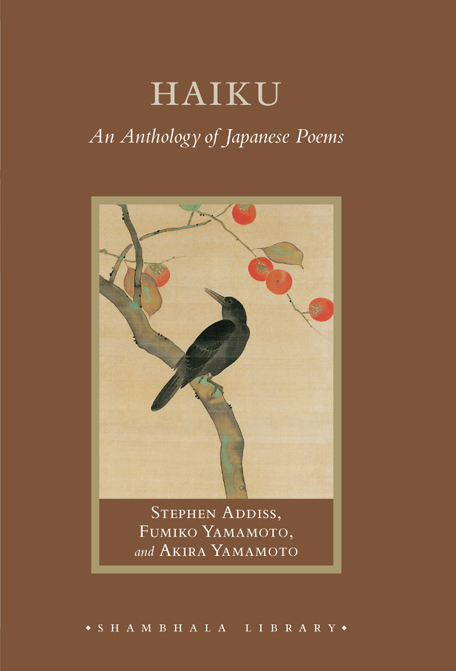
\includegraphics[width=\textwidth]{anthology}
\end{figure}

\chapter{Introduction}

\begin{figure}
    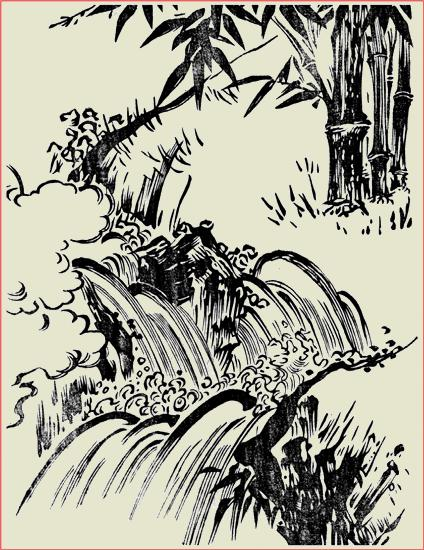
\includegraphics[width=\textwidth]{anthology-01}
\end{figure}

\setcounter{haikucounter}{0}

\begin{haiku}
    {\FH 夜の蘭香にかくれてや花白し}\hfill{\FH 蕪村}

    \vin{} Evening orchid ---
    \vin{} \vin{} is it hidden in its scent?
    \vin{} \vin{} \vin{} the white of its flower

\end{haiku}

\begin{haiku}
    {\FH まよひ子のをの\ruby{か}{が}太鼓\ruby{て}{で}\ruby{尋}{たずね}られ}\hfill{\FH 無名氏}

    \vin{} The lost child
    \vin{} \vin{} with his own drum
    \vin{} \vin{} \vin{} is searched for
\end{haiku}

\chapter{The Pulse of Nature}

\begin{figure}
    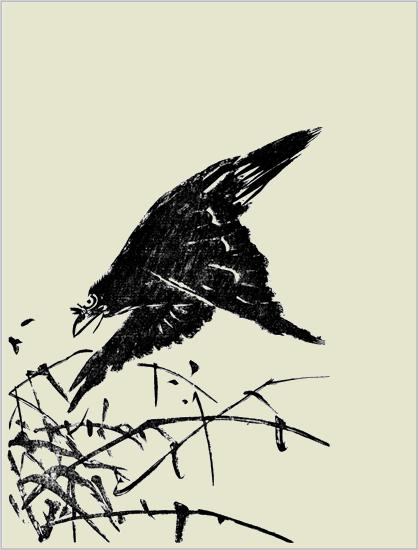
\includegraphics[width=\textwidth]{anthology-02}
\end{figure}

\begin{haiku}
    {\FH 打解けて氷と水の仲なほり}\hfill{\FH 貞室}

    \vin{} Opening their hearts
    \vin{} \vin{} ice and water become
    \vin{} \vin{} \vin{} friends again
    \hspace*{\fill} TEISHITSU
\end{haiku}

\begin{haiku}
    {\FH 春の日の\ruby{威光}{いこう}をみする雪間哉}\hfill{\FH 重頼}

    \vin{} The spring sun
    \vin{} \vin{} shows its power
    \vin{} \vin{} \vin{} between snowfalls \hspace{\fill} SHIGEYORI
\end{haiku}

\begin{haiku}
    {\FH ひたすらに咲うでもなし門の梅}\hfill{\FH 一茶}

    \vin{} Not in a hurry
    \vin{} \vin{} to blossom ---
    \vin{} \vin{} \vin{} plum tree at my gate \hspace{\fill} ISSA
\end{haiku}

\begin{haiku}
    {\FH しら梅の枯木にもどる月夜哉}\hfill{\FH 蕪村}

    \vin{} White plum blossoms
    \vin{} \vin{} return to the withered tree ---
    \vin{} \vin{} \vin{} moonlit night \hspace{\fill} BUSON
\end{haiku}

\begin{haiku}
    {\FH 鶯や泥足ぬぐふ梅の花}\hfill{\FH 一茶}

    \vin{} The warbler
    \vin{} \vin{} wipes its muddy feet
    \vin{} \vin{} \vin{} on plum blossoms \hspace{\fill} ISSA
\end{haiku}

\begin{haiku}
    {\FH 散るたびに老ゆく梅の木末かな}\hfill{\FH 蕪村}

    \vin{} With each falling petal
    \vin{} \vin{} they grow older ---
    \vin{} \vin{} \vin{} plum branches \hspace{\fill} BUSON
\end{haiku}

\begin{haiku}
    {\FH 枯芝ややゝ\ruby{陽炎}{かげろふ}の一二寸}\hfill{\FH 芭蕉}

    \vin{} Dried grasses ---
    \vin{} \vin{} and just a few heat waves
    \vin{} \vin{} \vin{} rising an inch or two \hspace{\fill} BASH\={O}
\end{haiku}

\begin{haiku}
    {\FH 愛あまる猫は傾婦の\ruby{媚}{こび}を仮る}\hfill{\FH 才麿}

    \vin{} Overflowing with love
    \vin{} \vin{} the cat as coquettish
    \vin{} \vin{} \vin{} as a courtesan \hspace{\fill} SAIMARO
\end{haiku}

\begin{haiku}
    {\FH 両方に髭があるなり猫の恋}\hfill{\FH 来山}

    \vin{} Both partners
    \vin{} \vin{} sport whiskers ---
    \vin{} \vin{} \vin{} cats' love \hspace{\fill} RAIZAN
\end{haiku}

\begin{haiku}
    {\FH 春の日や水さへあれば暮残り}\hfill{\FH 一茶}

    \vin{} Spring sun
    \vin{} \vin{} in every pool of water ---
    \vin{} \vin{} \vin{} lingering \hspace{\fill} ISSA
\end{haiku}

\begin{haiku}
    {\FH 曉も埋めたまゝや朧月}\hfill{\FH 鳥酔}

    \vin{} Is the dawn, too,
    \vin{} \vin{} still embraced by
    \vin{} \vin{} \vin{} hazy moon? \hspace{\fill} CH\={O}SUI
\end{haiku}

\begin{haiku}
    {\FH 陽炎に何やら猫の寝言哉}\hfill{\FH 一茶}

    \vin{} In the shimmering haze
    \vin{} \vin{} the cat mumbles something
    \vin{} \vin{} \vin{} in its sleep \hspace{\fill} ISSA
\end{haiku}

\begin{haiku}
    {\FH 春雨や小磯の小貝ぬるるほど}\hfill{\FH 蕪村}

    \vin{} Spring rain ---
    \vin{} \vin{} just enough to wet tiny shells
    \vin{} \vin{} \vin{} on the tiny beach \hspace{\fill} BUSON
\end{haiku}

\begin{figure}
    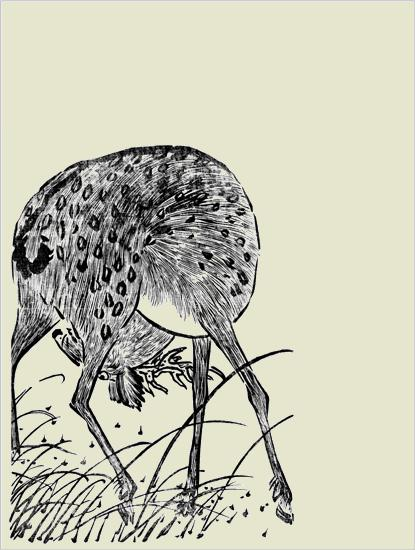
\includegraphics[width=\textwidth]{anthology-03}
\end{figure}

\begin{haiku}
    {\FH \ruby{植木}{うえき}屋のおいて行たる胡蝶かな}\hfill{\FH 蓼太}

    \vin{} The nurseryman
    \vin{} \vin{} left behind
    \vin{} \vin{} \vin{} a butterfly \hspace{\fill} RY\={O}TA
\end{haiku}

\begin{haiku}
    {\FH くりかへし麦の\ruby{畝}{うね}ぬふ小蝶かな}\hfill{\FH 曾良}

    \vin{} Again and again
    \vin{} \vin{} stitching the rows of barley ---
    \vin{} \vin{} \vin{} a butterfly \hspace{\fill} SORA
\end{haiku}

\begin{haiku}
    {\FH 雉の尾のやさしくさはる菫かな}\hfill{\FH 秋色女}

    \vin{} A pheasant's tail
    \vin{} \vin{} very gently brushes
    \vin{} \vin{} \vin{} the violets \hspace{\fill} SH\={U}SHIKI-JO
\end{haiku}

\begin{haiku}
    {\FH 菫越して小さき風の渡りけり}\hfill{\FH 温亭}

    \vin{} Over the violets
    \vin{} \vin{} a small breeze
    \vin{} \vin{} \vin{} passes by \hspace{\fill} ONTEI
\end{haiku}

\begin{haiku}
    {\FH 吹くたびに蝶のゐなほる柳かな}\hfill{\FH 芭蕉}

    \vin{} Each time the wind blows
    \vin{} \vin{} the butterfly sits anew
    \vin{} \vin{} \vin{} on the willow \hspace{\fill} BASH\={O}
\end{haiku}

\begin{haiku}
    {\FH 春寒し水田の上の根さし雲}\hfill{\FH 碧梧桐}

    \vin{} Spring chill ---
    \vin{} \vin{} above the rice paddies
    \vin{} \vin{} \vin{} rootless clouds \hspace{\fill} HEKIGOD\={O}
\end{haiku}

\begin{haiku}
    {\FH あけぼのや白魚白きこと一寸}\hfill{\FH 芭蕉}

    \vin{} Daybreak ---
    \vin{} \vin{} the whitefish whiten
    \vin{} \vin{} \vin{} only one inch \hspace{\fill} BASH\={O}
\end{haiku}

\begin{haiku}
    {---}\hfill{---}

    \vin{} Domestic ducks
    \vin{} \vin{} stretch their necks
    \vin{} \vin{} \vin{} hoping to see the world \hspace{\fill} K\={O}JI
\end{haiku}

\begin{haiku}
    {\FH 鶯の笠\ruby{落}{おと}したる椿かな}\hfill{\FH 芭蕉}

    \vin{} The warbler
    \vin{} \vin{} dropped his hat ---
    \vin{} \vin{} \vin{} a camellia \hspace{\fill} BASH\={O}
\end{haiku}

\begin{haiku}
    {\FH 花に狂ひ月に驚く胡蝶かな}\hfill{\FH 樗良}

    \vin{} Crazed by flowers
    \vin{} \vin{} surprised by the moon ---
    \vin{} \vin{} \vin{} a butterfly \hspace{\fill} CHORA
\end{haiku}

\begin{haiku}
    {\FH 白椿落つる音のみ月夜かな}\hfill{\FH 闌更}

    \vin{} White camellias ---
    \vin{} \vin{} only the sound of their falling
    \vin{} \vin{} \vin{} moonlit night \hspace{\fill} RANK\={O}
\end{haiku}

\begin{haiku}
    {\FH 雀子と声鳴きかはす鼠の巣}\hfill{\FH 芭蕉}

    \vin{} Squeaking in response
    \vin{} \vin{} to baby sparrows ---
    \vin{} \vin{} \vin{} a nest of mice \hspace{\fill} BASH\={O}
\end{haiku}

\begin{figure}
    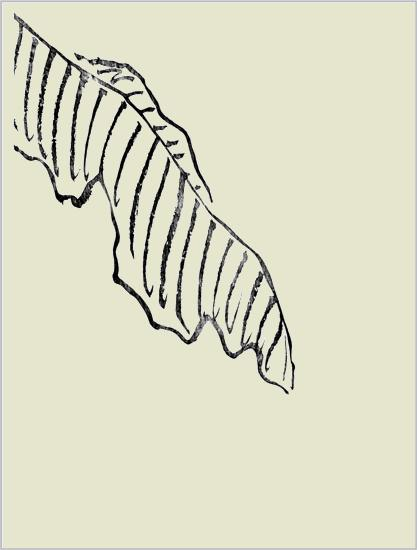
\includegraphics[width=\textwidth]{anthology-04}
\end{figure}

\begin{haiku}
    {\FH \ruby{闇}{くらき}より闇に入るや猫の恋}\hfill{\FH 一茶}

    \vin{} Out from the darkness
    \vin{} \vin{} back into the darkness ---
    \vin{} \vin{} \vin{} affairs of the cat \hspace{\fill} ISSA
\end{haiku}

\begin{haiku}
    {\FH 夜はうれしく昼は静なり春の雨}\hfill{\FH 樗良}

    \vin{} Joyful at night
    \vin{} \vin{} tranquil during the day ---
    \vin{} \vin{} \vin{} spring rain \hspace{\fill} CHORA
\end{haiku}

\begin{haiku}
    {\FH 椿落て昨日の雨をこぼしけり}\hfill{\FH 蕪村}

    \vin{} A camellia falls
    \vin{} \vin{} spilling out
    \vin{} \vin{} \vin{} yesterday's rain \hspace{\fill} BUSON
\end{haiku}

\begin{haiku}
    {\FH 茨\ruby{垣}{かき}犬の上手に\ruby{潜}{くぐ}りけり}\hfill{\FH 一茶}

    \vin{} A hedge of thorns ---
    \vin{} \vin{} how skillfully the dog
    \vin{} \vin{} \vin{} wriggled under it! \hspace{\fill} ISSA
\end{haiku}

\begin{haiku}
    {\FH かすむ日の咄するやらのべの馬}\hfill{\FH 一茶}

    \vin{} Misty day ---
    \vin{} \vin{} they might be gossiping
    \vin{} \vin{} \vin{} horses in the field \hspace{\fill} ISSA
\end{haiku}

\begin{haiku}
    {\FH 古井戸の暗きに落る椿かな}\hfill{\FH 蕪村}

    \vin{} An old well ---
    \vin{} \vin{} falling into its darkness
    \vin{} \vin{} \vin{} a camellia \hspace{\fill} BUSON
\end{haiku}

\begin{haiku}
    {\FH 雲をふみ霞を吸うやあげ雲雀}\hfill{\FH 子規}

    \vin{} Trampling on clouds,
    \vin{} \vin{} inhaling the mist,
    \vin{} \vin{} \vin{} the skylark soars \hspace{\fill} SHIKI
\end{haiku}

\begin{haiku}
    {\FH \ruby{踞}{うずく}\ruby{ふ}{ば}て雲を\ruby{伺}{うかが}ふ蛙かな}\hfill{\FH 千代女}

    \vin{} Crouching,
    \vin{} \vin{} studying the clouds ---
    \vin{} \vin{} \vin{} a frog \hspace{\fill} CHIYO-JO
\end{haiku}

\begin{haiku}
    {\FH 釣鐘にとまりて眠る胡蝶かな}\hfill{\FH 蕪村}

    \vin{} On the temple bell
    \vin{} \vin{} perching and sleeping ---
    \vin{} \vin{} \vin{} a butterfly \hspace{\fill} BUSON
\end{haiku}

\begin{haiku}
    {\FH \ruby{釋教}{しゃっきょう}の歌か寺井に鳴くかへる}\hfill{\FH 閑節}

    \vin{} Could they be sutras?
    \vin{} \vin{} in the temple well
    \vin{} \vin{} \vin{} frogs chant \hspace{\fill} KANSETSU
\end{haiku}

\begin{haiku}
    {\FH 長く鳴く蛙の歌や文字\ruby{余}{あま}り}\hfill{\FH 永治}

    \vin{} Recited on and on,
    \vin{} \vin{} the poems of the frogs
    \vin{} \vin{} \vin{} have too many syllables \hspace{\fill} EIJI
\end{haiku}

\begin{haiku}
    {\FH 手をついて歌申しあぐる蛙かな}\hfill{\FH 宗鑑}

    \vin{} Bracing his feet
    \vin{} \vin{} and offering up a song ---
    \vin{} \vin{} \vin{} the frog \hspace{\fill} S\={O}KAN
\end{haiku}

\begin{haiku}
    {\FH 大仏の鼻から出たる\ruby{乙鳥}{つばめ}哉}\hfill{\FH 一茶}

    \vin{} From the nostril
    \vin{} \vin{} of the Great Buddha comes
    \vin{} \vin{} \vin{} a swallow \hspace{\fill} ISSA
\end{haiku}

\begin{figure}
    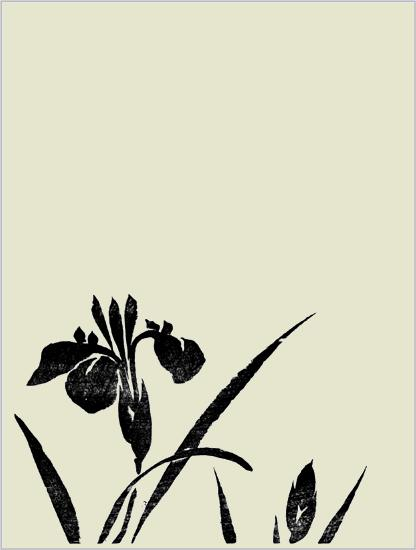
\includegraphics[width=\textwidth]{anthology-05}
\end{figure}

\begin{haiku}
    {\FH \ruby{柴門}{しばのと}や錠のかはりのかたつぶり}\hfill{\FH 一茶}

    \vin{} On the brushwood gate
    \vin{} \vin{} in place of a lock ---
    \vin{} \vin{} \vin{} one snail \hspace{\fill} ISSA
\end{haiku}

\begin{haiku}
    {\FH 日の影や眠れる蝶に\ruby{透}{す}き通り}\hfill{\FH 闌更}

    \vin{} Sunlight
    \vin{} \vin{} passes through a butterfly
    \vin{} \vin{} \vin{} asleep \hspace{\fill} RANK\={O}
\end{haiku}

\begin{haiku}
    {\FH 取りつかぬ心で\ruby{浮}{う}かむ蛙かな}\hfill{\FH 丈草}

    \vin{} With the power of non-attachment
    \vin{} \vin{} floating on the water ---
    \vin{} \vin{} \vin{} a frog \hspace{\fill} J\={O}S\={O}
\end{haiku}

\begin{haiku}
    {\FH 花を照らし月また花にくもる哉}\hfill{\FH 樗良}

    \vin{} Highlighting the blossoms,
    \vin{} \vin{} clouded by blossoms ---
    \vin{} \vin{} \vin{} the moon \hspace{\fill} CHORA
\end{haiku}

\begin{haiku}
    {\FH 花びらの山を動かす桜かな}\hfill{\FH 抱一}

    \vin{} Flower petals
    \vin{} \vin{} set the mountain in motion ---
    \vin{} \vin{} \vin{} cherry blossoms \hspace{\fill} H\={O}ITSU
\end{haiku}

\begin{haiku}
    {\FH 一めんの\ruby{落花}{らっか}の水に蛙の眼}\hfill{\FH 風生}

    \vin{} On the surface
    \vin{} \vin{} of petal-covered water ---
    \vin{} \vin{} \vin{} frogs' eyes \hspace{\fill} F\={U}SEI
\end{haiku}

\begin{haiku}
    {\FH 行く春のうしろ姿や藤の花}\hfill{\FH 可南女}

    \vin{} The retreating shapes
    \vin{} \vin{} of the passing spring ---
    \vin{} \vin{} \vin{} wisteria \hspace{\fill} KANA-JO
\end{haiku}

\begin{haiku}
    {\FH 行春や\ruby{逡}{しゆん}\ruby{巡}{じゆん}として遅ざくら}\hfill{\FH 蕪村}

    \vin{} Spring passes ---
    \vin{} \vin{} the last reluctant
    \vin{} \vin{} \vin{} cherry blossoms \hspace{\fill} BUSON
\end{haiku}

\begin{figure}
    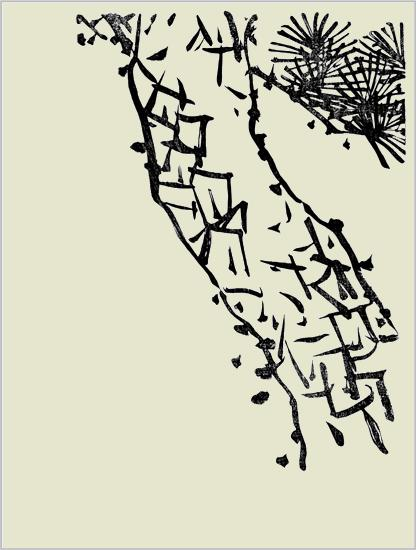
\includegraphics[width=\textwidth]{anthology-06}
\end{figure}

\begin{haiku}
    {\FH 浅河の西し東シす若葉哉}\hfill{\FH 蕪村}

    \vin{} Shallow river
    \vin{} \vin{} twisting west and twisting east ---
    \vin{} \vin{} \vin{} young leaves \hspace{\fill} BUSON
\end{haiku}

\begin{haiku}
    {\FH \ruby{連翹}{れんぎょう}のまぶしき春の\ruby{憂}{うれ}ひかな}\hfill{\FH 万太郎}

    \vin{} Forsythia ---
    \vin{} \vin{} and radiant spring's
    \vin{} \vin{} \vin{} melancholy \hspace{\fill} MANTAR\={O}
\end{haiku}

\begin{haiku}
    {\FH 日は日くれよ夜は夜明ケよと啼蛙}\hfill{\FH 蕪村}

    \vin{} In daytime ``darken the day''
    \vin{} \vin{} at night ``brighten the night''
    \vin{} \vin{} \vin{} frogs chant \hspace{\fill} BUSON
\end{haiku}

\begin{haiku}
    {\FH 海越て霞の網に入日哉}\hfill{\FH 蕪村}

    \vin{} Crossing the sea
    \vin{} \vin{} into a net of mist ---
    \vin{} \vin{} \vin{} the setting sun \hspace{\fill} BUSON
\end{haiku}

\begin{haiku}
    {\FH 草霞み水に声なき日ぐれ哉}\hfill{\FH 蕪村}

    \vin{} Misty grasses ---
    \vin{} \vin{} water without voices
    \vin{} \vin{} \vin{} in the dusk \hspace{\fill} BUSON
\end{haiku}

\begin{haiku}
    {\FH 行く春や海を見て居る鴉の子}\hfill{\FH 諸九}

    \vin{} Spring passing ---
    \vin{} \vin{} looking at the sea,
    \vin{} \vin{} \vin{} a baby crow \hspace{\fill} SHOKY\={U}
\end{haiku}

\begin{haiku}
    {\FH \ruby{郭公}{ほととぎす}一声夏をさだめけり}\hfill{\FH 蓼太}

    \vin{} The cuckoo
    \vin{} \vin{} with a single song
    \vin{} \vin{} \vin{} has established summer \hspace{\fill} RY\={O}TA
\end{haiku}

\begin{haiku}
    {\FH ほととぎす声や横たふ水の上}\hfill{\FH 芭蕉}

    \vin{} The voice of the cuckoo
    \vin{} \vin{} slants
    \vin{} \vin{} \vin{} over the water \hspace{\fill} BASH\={O}
\end{haiku}

\begin{haiku}
    {\FH 郭公鳴くや湖水のささにごり}\hfill{\FH 丈草}

    \vin{} The cuckoo calls ---
    \vin{} \vin{} and the waters of the lake
    \vin{} \vin{} \vin{} cloud over a little \hspace{\fill} J\={O}S\={O}
\end{haiku}

\begin{haiku}
    {\FH 時鳥蝿虫めらもよっく聞け}\hfill{\FH 一茶}

    \vin{} The cuckoo ---
    \vin{} \vin{} flies and insects,
    \vin{} \vin{} \vin{} listen well! \hspace{\fill} ISSA
\end{haiku}

\begin{haiku}
    {\FH 五月雨や梅の葉寒き風の色}\hfill{\FH 才麿}

    \vin{} Summer rains ---
    \vin{} \vin{} leaves of the plum
    \vin{} \vin{} \vin{} the color of cold wind \hspace{\fill} SAIMARO
\end{haiku}

\begin{haiku}
    {\FH 五月雨や滄海を衝く濁水}\hfill{\FH 蕪村}

    \vin{} Early summer rains ---
    \vin{} \vin{} lunging at the blue sea
    \vin{} \vin{} \vin{} muddy waters \hspace{\fill} BUSON
\end{haiku}

\begin{figure}
    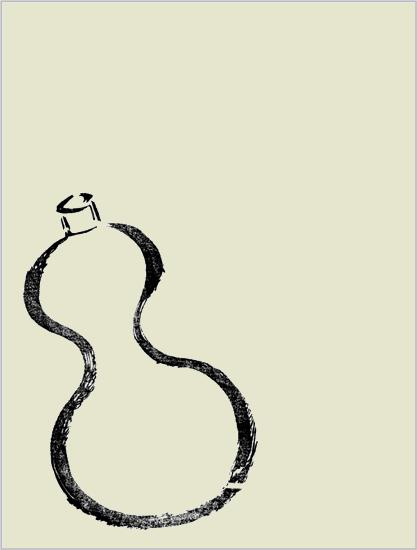
\includegraphics[width=\textwidth]{anthology-07}
\end{figure}

\begin{haiku}
    {\FH 五月雨の名もなき川のおそろしき}\hfill{\FH 蕪村}

    \vin{} Early summer rains ---
    \vin{} \vin{} even nameless rivers
    \vin{} \vin{} \vin{} are fearsome \hspace{\fill} BUSON
\end{haiku}

\begin{haiku}
    {\FH 涼しさや青田の中の一つ松}\hfill{\FH 子規}

    \vin{} Summer cool ---
    \vin{} \vin{} in the green rice fields
    \vin{} \vin{} \vin{} a single pine \hspace{\fill} SHIKI
\end{haiku}

\begin{haiku}
    {\FH 不二ひとつ埋み残して若葉かな}\hfill{\FH 蕪村}

    \vin{} Only Fuji
    \vin{} \vin{} remains unburied ---
    \vin{} \vin{} \vin{} young leaves \hspace{\fill} BUSON
\end{haiku}

\begin{haiku}
    {\FH 紫陽花におもたき朝日夕日哉}\hfill{\FH 乙由}

    \vin{} On the hydrangeas
    \vin{} \vin{} the weight of the morning sun,
    \vin{} \vin{} \vin{} the evening sun \hspace{\fill} OTSUY\={U}
\end{haiku}

\begin{haiku}
    {\FH 山蟻のあからさま也白牡丹}\hfill{\FH 蕪村}

    \vin{} Mountain ant ---
    \vin{} \vin{} seen so clearly
    \vin{} \vin{} \vin{} on the white peony \hspace{\fill} BUSON
\end{haiku}

\begin{haiku}
    {\FH ひとりひつそり竹の子竹になる}\hfill{\FH 山頭火}

    \vin{} Alone, silently ---
    \vin{} \vin{} the bamboo shoot
    \vin{} \vin{} \vin{} becomes a bamboo \hspace{\fill} SANT\={O}KA
\end{haiku}

\begin{haiku}
    {\FH 鶯や竹の子薮に老を鳴く}\hfill{\FH 芭蕉}

    \vin{} The warbler
    \vin{} \vin{} amid the bamboo shoots
    \vin{} \vin{} \vin{} sings of old age \hspace{\fill} BASH\={O}
\end{haiku}

\begin{haiku}
    {\FH 三角のいとま\ruby{蜥蜴}{とかげ}の顔の少し延ぶか}\hfill{\FH 虚子}

    \vin{} A triangle ---
    \vin{} \vin{} is the lizard's head getting
    \vin{} \vin{} \vin{} a little longer? \hspace{\fill} KYOSHI
\end{haiku}

\begin{haiku}
    {\FH 我宿や鼠と仲のよい蛍}\hfill{\FH 一茶}

    \vin{} In my dwelling
    \vin{} \vin{} friendly with the mice ---
    \vin{} \vin{} \vin{} fireflies \hspace{\fill} ISSA
\end{haiku}

\begin{haiku}
    {\FH おもしろや左右の使の飛ぶほたる}\hfill{\FH 介我}

    \vin{} How interesting ---
    \vin{} \vin{} running errands right and left
    \vin{} \vin{} \vin{} fireflies \hspace{\fill} KAIGA
\end{haiku}

\begin{haiku}
    {\FH 追れては月にかくるるほたる哉}\hfill{\FH 蓼太}

    \vin{} Pursued,
    \vin{} \vin{} it hides in the moon ---
    \vin{} \vin{} \vin{} the firefly \hspace{\fill} RY\={O}TA
\end{haiku}

\begin{haiku}
    {\FH もえやすく又消やすき蛍哉}\hfill{\FH 千子女}

    \vin{} Burning so easily,
    \vin{} \vin{} extinguishing so easily ---
    \vin{} \vin{} \vin{} the firefly \hspace{\fill} CHINE-JO
\end{haiku}

\begin{haiku}
    {\FH 朝風に毛を\ruby{吹}{ふか}れ居る毛むし哉}\hfill{\FH 蕪村}

    \vin{} The morning breeze
    \vin{} \vin{} ripples the fur
    \vin{} \vin{} \vin{} of the caterpillar \hspace{\fill} BUSON
\end{haiku}

\begin{figure}
    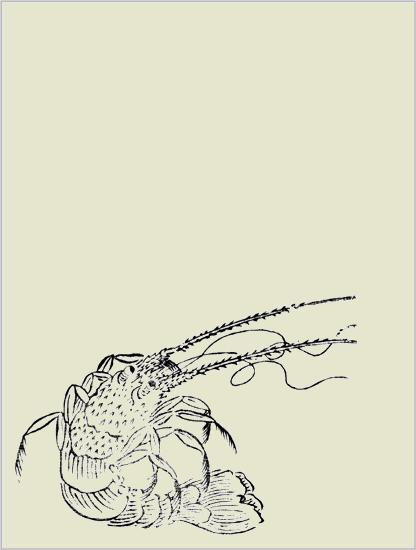
\includegraphics[width=\textwidth]{anthology-08}
\end{figure}

\begin{haiku}
    {\FH 湖に尻を吹かせて蝉の鳴}\hfill{\FH 一茶}

    \vin{} As the lake breeze
    \vin{} \vin{} cools his bottom
    \vin{} \vin{} \vin{} the cicada cries \hspace{\fill} ISSA
\end{haiku}

\begin{haiku}
    {\FH 稲妻につむりなでけり\ruby{引蟇}{ひきがえる}}\hfill{\FH 一茶}

    \vin{} As lightning flashes
    \vin{} \vin{} he strokes his head ---
    \vin{} \vin{} \vin{} the toad \hspace{\fill} ISSA
\end{haiku}

\begin{haiku}
    {\FH 蛇逃げて我を見し眼の草に残る}\hfill{\FH 虚子}

    \vin{} The snake flees ---
    \vin{} \vin{} but the eyes that peered at me
    \vin{} \vin{} \vin{} remain in the weeds \hspace{\fill} KYOSHI
\end{haiku}

\begin{haiku}
    {\FH さはさはと蓮うごかす池の亀}\hfill{\FH 鬼貫}

    \vin{} Rustling, rustling,
    \vin{} \vin{} the lotus leaves sway ---
    \vin{} \vin{} \vin{} a tortoise in the pond \hspace{\fill} ONITSURA
\end{haiku}

\begin{haiku}
    {\FH けふの日も棒ふり虫よ翌も又}\hfill{\FH 一茶}

    \vin{} Today too
    \vin{} \vin{} mosquito larvae ---
    \vin{} \vin{} \vin{} and tomorrow again \hspace{\fill} ISSA
\end{haiku}

\begin{haiku}
    {---}\hfill{\FH 無名氏}

    \vin{} As flies retreat
    \vin{} \vin{} mosquitoes start
    \vin{} \vin{} \vin{} their battle cry \hspace{\fill} ANONYMOUS
\end{haiku}

\begin{haiku}
    {---}\hfill{\FH 無名氏}

    \vin{} Dashing into one another
    \vin{} \vin{} whispering, parting ---
    \vin{} \vin{} \vin{} ants \hspace{\fill} ANONYMOUS
\end{haiku}

\begin{haiku}
    {雲を吐き雲を吸い込む峰の松}\hfill{\FH 無名氏}

    \vin{} Inhaling clouds
    \vin{} \vin{} exhaling clouds ---
    \vin{} \vin{} \vin{} mountaintop pines \hspace{\fill} ANONYMOUS
\end{haiku}

\begin{figure}
    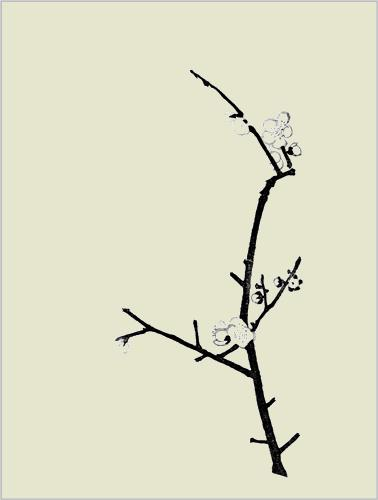
\includegraphics[width=\textwidth]{anthology-09}
\end{figure}

\begin{haiku}
    {\FH 蚊\ruby{柱}{ばしら}に夢の浮橋かかるなり}\hfill{\FH 其角}

    \vin{} Across a pillar of mosquitoes
    \vin{} \vin{} hangs the bridge
    \vin{} \vin{} \vin{} of dreams \hspace{\fill} KIKAKU
\end{haiku}

\begin{haiku}
    {\FH 蛤の口しめてゐる暑さかな}\hfill{\FH 芭蕉}

    \vin{} Even the clams
    \vin{} \vin{} keep their mouths shut
    \vin{} \vin{} \vin{} in this heat \hspace{\fill} BASH\={O}
\end{haiku}

\begin{haiku}
    {\FH 古壁の隅に動かずはらみ蜘}\hfill{\FH 子規}

    \vin{} Motionless
    \vin{} \vin{} in a crevice of an old wall ---
    \vin{} \vin{} \vin{} a pregnant spider \hspace{\fill} SHIKI
\end{haiku}

\begin{haiku}
    {\FH \ruby{濤}{なみ}暑し石に\ruby{怒}{いか}れるひびきあり}\hfill{\FH 暁台}

    \vin{} Heat in waves ---
    \vin{} \vin{} in the stones
    \vin{} \vin{} \vin{} angry reverberations \hspace{\fill} KY\={O}TAI
\end{haiku}

\begin{haiku}
    {\FH ゆふ立やよみがへりたる\ruby{斃}{たおれ}馬}\hfill{\FH 几董}

    \vin{} Sudden shower ---
    \vin{} \vin{} and rising from the heat,
    \vin{} \vin{} \vin{} the broken-down horse \hspace{\fill} KIT\={O}
\end{haiku}

\begin{haiku}
    ---\hfill{---}

    \vin{} Lightning!
    \vin{} \vin{} fleeing up the wall,
    \vin{} \vin{} \vin{} the legs of a spider \hspace{\fill} KICH\={O}
\end{haiku}

\begin{haiku}
    {\FH 夕立や草葉をつかむむら雀}\hfill{\FH 蕪村}

    \vin{} Sudden shower ---
    \vin{} \vin{} clutching the blades of grass
    \vin{} \vin{} \vin{} a flock of sparrows \hspace{\fill} BUSON
\end{haiku}

\begin{haiku}
    {\FH 桐の木や雨のながるる蝉の腹}\hfill{\FH 梅室}

    \vin{} Down a paulownia tree
    \vin{} \vin{} the rain comes trickling
    \vin{} \vin{} \vin{} across a cicada's belly \hspace{\fill} BAISHITSU
\end{haiku}

\begin{haiku}
    {\FH \ruby{雨蛙}{あまがえる}芭蕉にのりてそよぎけり}\hfill{\FH 其角}

    \vin{} The tree frog
    \vin{} \vin{} riding the plantain leaf
    \vin{} \vin{} \vin{} sways \hspace{\fill} KIKAKU
\end{haiku}

\begin{haiku}
    {\FH ばか長い日やと口明く烏哉}\hfill{\FH 一茶}

    \vin{} ``It's much too long a day'',
    \vin{} \vin{} opening its mouth
    \vin{} \vin{} \vin{} a crow \hspace{\fill} ISSA
\end{haiku}

\begin{haiku}
    {\FH 魚どもは桶としらでや夕涼}\hfill{\FH 一茶}

    \vin{} The fish
    \vin{} \vin{} not knowing they're in a bucket
    \vin{} \vin{} \vin{} cool by the gate \hspace{\fill} ISSA
\end{haiku}

\begin{haiku}
    {\FH 夕立にうたるゝ鯉のかしらかな}\hfill{\FH 子規}

    \vin{} A sudden shower
    \vin{} \vin{} drums down upon
    \vin{} \vin{} \vin{} the heads of the carp \hspace{\fill} SHIKI
\end{haiku}

\begin{haiku}
    {\FH いなづまやきのふは東けふは西}\hfill{\FH 其角}

    \vin{} Lightning ---
    \vin{} \vin{} yesterday to the east
    \vin{} \vin{} \vin{} today to the west \hspace{\fill} KIKAKU
\end{haiku}

\begin{haiku}
    {\FH 一本の草も涼風やどりけり}\hfill{\FH 一茶}

    \vin{} Even in a single blade of grass
    \vin{} \vin{} the cool breeze
    \vin{} \vin{} \vin{} finds a home \hspace{\fill} ISSA
\end{haiku}

\begin{haiku}
    {\FH 飛ぶ鮎の底に雲ゆく流かな}\hfill{\FH 鬼貫}

    \vin{} The trout leaps up ---
    \vin{} \vin{} and below him in a stream
    \vin{} \vin{} \vin{} clouds float by \hspace{\fill} ONITSURA
\end{haiku}

\begin{haiku}
    {\FH しづかさや湖水の底の雲のみね}\hfill{\FH 一茶}

    \vin{} How quiet ---
    \vin{} \vin{} at the bottom of the lake
    \vin{} \vin{} \vin{} peaks of clouds \hspace{\fill} ISSA
\end{haiku}

\begin{haiku}
    {\FH 海の音にひまわり黒き瞳をひらく}\hfill{\FH 夕爾}

    \vin{} At the sound of the sea
    \vin{} \vin{} the sunflowers open
    \vin{} \vin{} \vin{} their black eyes \hspace{\fill} Y\={U}JI
\end{haiku}

\begin{haiku}
    {\FH 蛸壺やはかなき夢を夏の月}\hfill{\FH 芭蕉}

    \vin{} Octopus pot ---
    \vin{} \vin{} evanescent dreams
    \vin{} \vin{} \vin{} of the summer moon \hspace{\fill} BASH\={O}
\end{haiku}

\begin{haiku}
    {\FH 短夜や\ruby{芦}{あし}間流るる蟹の\ruby{泡}{あわ}}\hfill{\FH 蕪村}

    \vin{} Short summer night ---
    \vin{} \vin{} flowing through reeds
    \vin{} \vin{} \vin{} bubbles from crabs \hspace{\fill} BUSON
\end{haiku}

\begin{haiku}
    {\FH 閑さや岩にしみ入る蝉の声}\hfill{\FH 芭蕉}

    \vin{} Stillness ---
    \vin{} \vin{} seeping into the rocks
    \vin{} \vin{} \vin{} the cicada's voice \hspace{\fill} BASH\={O}
\end{haiku}

\begin{haiku}
    {\FH うつくしく牛の痩せたる夏野哉}\hfill{\FH 凡兆}

    \vin{} How beautifully
    \vin{} \vin{} the cow has slimmed down
    \vin{} \vin{} \vin{} in the summer fields \hspace{\fill} BONCH\={O}
\end{haiku}

\begin{haiku}
    {\FH 朝露や撫でて涼しき瓜の土}\hfill{\FH 芭蕉}

    \vin{} In the morning dew
    \vin{} \vin{} soiled and cooled ---
    \vin{} \vin{} \vin{} dirt on the melon \hspace{\fill} BASH\={O}
\end{haiku}

\begin{figure}
    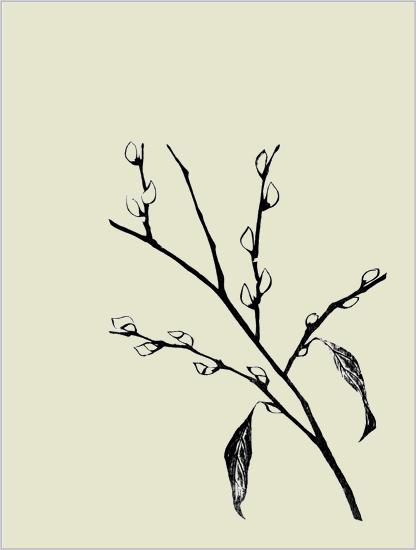
\includegraphics[width=\textwidth]{anthology-10}
\end{figure}

\begin{haiku}
    {\FH 涼しさや\ruby{行燈}{あん}どん消えて水の音}\hfill{\FH 子規}

    \vin{} Summer coolness ---
    \vin{} \vin{} lantern out,
    \vin{} \vin{} \vin{} the sound of water \hspace{\fill} SHIKI
\end{haiku}

\begin{haiku}
    {\FH 五月雨やある夜ひそかに松の月}\hfill{\FH 蓼太}

    \vin{} Summer rains ---
    \vin{} \vin{} secretly one evening
    \vin{} \vin{} \vin{} moon in the pines \hspace{\fill} RY\={O}TA
\end{haiku}

\begin{haiku}
    {\FH かはほりのかくれ住けり破れ傘}\hfill{\FH 蕪村}

    \vin{} The bat's
    \vin{} \vin{} secret home ---
    \vin{} \vin{} \vin{} a tattered hat \hspace{\fill} BUSON
\end{haiku}

\begin{haiku}
    {\FH 夕顔の花\ruby{噛}{か}む猫や余所ごころ}\hfill{\FH 蕪村}

    \vin{} Evening glories ---
    \vin{} \vin{} the cat chewing the flower
    \vin{} \vin{} \vin{} has its mind elsewhere \hspace{\fill} BUSON
\end{haiku}

\begin{haiku}
    {\FH 麦のほに尾を隠さばや老狐}\hfill{\FH 轍士}

    \vin{} Among the ears of barley
    \vin{} \vin{} are you hiding your tail?
    \vin{} \vin{} \vin{} old fox \hspace{\fill} TESSHI
\end{haiku}

\begin{haiku}
    {\FH 秋の季の赤とんぼうに\ruby{定}{さだ}まりぬ}\hfill{\FH 白雄}

    \vin{} The coming of autumn
    \vin{} \vin{} determined
    \vin{} \vin{} \vin{} by a red dragonfly \hspace{\fill} SHIRAO
\end{haiku}

\begin{haiku}
    {---}\hfill{\FH 紅葉}

    \vin{} The stars
    \vin{} \vin{} have already opened
    \vin{} \vin{} \vin{} their autumn eyes \hspace{\fill} K\={O}Y\={O}
\end{haiku}

\begin{haiku}
    {\FH 初秋や夕立長引く夜の雨}\hfill{\FH 太祇}

    \vin{} Early autumn ---
    \vin{} \vin{} the evening shower becomes
    \vin{} \vin{} \vin{} a night of rain \hspace{\fill} TAIGI
\end{haiku}

\begin{haiku}
    {\FH 初秋や海も青田も一みどり}\hfill{\FH 芭蕉}

    \vin{} Autumn begins ---
    \vin{} \vin{} ocean and fields
    \vin{} \vin{} \vin{} all one green \hspace{\fill} BASH\={O}
\end{haiku}

\begin{haiku}
    {\FH はや秋の柳をすかす朝日かな}\hfill{\FH 成美}

    \vin{} Early autumn ---
    \vin{} \vin{} peering through willows
    \vin{} \vin{} \vin{} the morning sun \hspace{\fill} SEIBI
\end{haiku}

\begin{haiku}
    {\FH 朝顔や吹倒されたなりに咲}\hfill{\FH 一茶}

    \vin{} Morning glories ---
    \vin{} \vin{} blown to the ground
    \vin{} \vin{} \vin{} bloom as they are \hspace{\fill} ISSA
\end{haiku}

\begin{haiku}
    {\FH 露ほろりほろと鳩の念仏哉}\hfill{\FH 一茶}

    \vin{} As dew drips
    \vin{} \vin{} gently, gently, the dove
    \vin{} \vin{} \vin{} murmurs its chant \hspace{\fill} ISSA
\end{haiku}

\begin{haiku}
    {\FH 草も木も月待つ露の夕かな}\hfill{\FH 宗祇}

    \vin{} Grasses and trees all
    \vin{} \vin{} waiting for the moon ---
    \vin{} \vin{} \vin{} dewy evening \hspace{\fill} S\={O}GI
\end{haiku}

\begin{figure}
    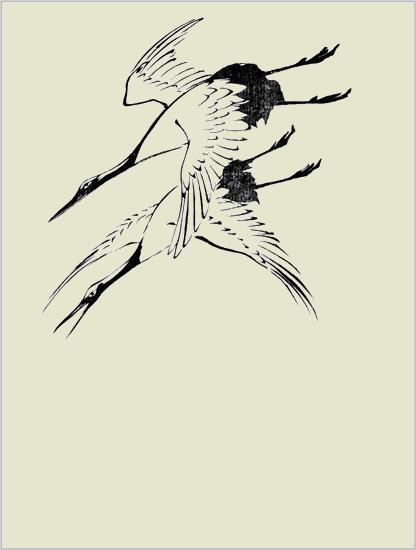
\includegraphics[width=\textwidth]{anthology-11}
\end{figure}

\begin{haiku}
    {\FH 白露や茨のとげにひとつずつ}\hfill{\FH 蕪村}

    \vin{} White dew
    \vin{} \vin{} on brambles and thorns ---
    \vin{} \vin{} \vin{} one drop each \hspace{\fill} BUSON
\end{haiku}

\begin{haiku}
    {\FH \ruby{艸}{くさ}の葉を遊びありけよ露の玉}\hfill{\FH 嵐雪}

    \vin{} On blades of grass
    \vin{} \vin{} frolic and roll on ---
    \vin{} \vin{} \vin{} pearls of dew \hspace{\fill} RANSETSU
\end{haiku}

\begin{haiku}
    {\FH 露凉し形あるもの皆生ける}\hfill{\FH 鬼城}

    \vin{} Dew cooling ---
    \vin{} \vin{} things with shapes
    \vin{} \vin{} \vin{} all alive \hspace{\fill} KIJ\={O}
\end{haiku}

\begin{haiku}
    {---}\hfill{\FH 無名氏}

    \vin{} Its face
    \vin{} \vin{} looks like a horse ---
    \vin{} \vin{} \vin{} the grasshopper \hspace{\fill} ANONYMOUS
\end{haiku}

\begin{haiku}
    {\FH 石にとんぼはまひるのゆめみる}\hfill{\FH 山頭火}

    \vin{} Dragonfly on a rock
    \vin{} \vin{} absorbed in
    \vin{} \vin{} \vin{} a daydream \hspace{\fill} SANT\={O}KA
\end{haiku}

\begin{haiku}
    {\FH 蜻蜒や取りつきかねし草の上}\hfill{\FH 芭蕉}

    \vin{} The dragonfly
    \vin{} \vin{} cannot come to rest
    \vin{} \vin{} \vin{} on the blades of grass \hspace{\fill} BASH\={O}
\end{haiku}

\begin{haiku}
    {\FH 猫の子のかくれんぼする萩の花}\hfill{\FH 一茶}

    \vin{} Kittens
    \vin{} \vin{} playing hide-and-seek
    \vin{} \vin{} \vin{} in the bush clover \hspace{\fill} ISSA
\end{haiku}

\begin{haiku}
    {\FH 蜻蛉やくるひ静まる三日の月}\hfill{\FH 其角}

    \vin{} Dragonflies
    \vin{} \vin{} quiet their mad darting ---
    \vin{} \vin{} \vin{} crescent moon \hspace{\fill} KIKAKU
\end{haiku}

\begin{figure}
    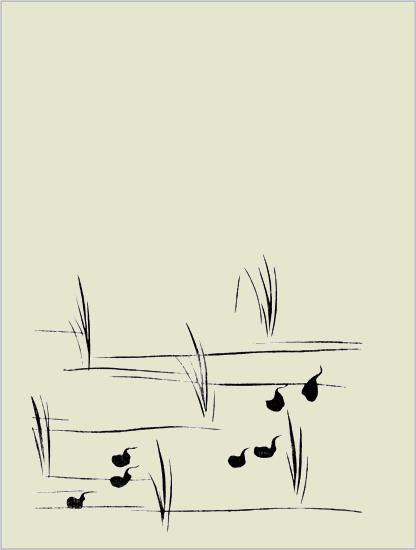
\includegraphics[width=\textwidth]{anthology-12}
\end{figure}

\begin{haiku}
    {\FH かはほりや月のあたりを立ちさらず}\hfill{\FH 暁台}

    \vin{} The bat
    \vin{} \vin{} circling the moon
    \vin{} \vin{} \vin{} would not leave it \hspace{\fill} KY\={O}TAI
\end{haiku}

\begin{haiku}
    {\FH 夢返せ烏の\ruby{覚}{さま}す霧の月}\hfill{\FH 鬼貫}

    \vin{} Give me back my dream!
    \vin{} \vin{} a crow has wakened me
    \vin{} \vin{} \vin{} to misty moonlight \hspace{\fill} ONITSURA
\end{haiku}

\begin{haiku}
    {\FH おのがみに秋を染め抜く蜻蛉かな}\hfill{\FH 麦水}

    \vin{} Dyeing his body
    \vin{} \vin{} autumn ---
    \vin{} \vin{} \vin{} the dragonfly \hspace{\fill} BAKUSUI
\end{haiku}

\begin{haiku}
    {\FH 遠山が目玉にうつるとんぼかな}\hfill{\FH 一茶}

    \vin{} Distant mountains
    \vin{} \vin{} reflecting in its eyes ---
    \vin{} \vin{} \vin{} a dragonfly \hspace{\fill} ISSA
\end{haiku}

\begin{haiku}
    {---}\hfill{\FH 無名氏}

    \vin{} A floating sandal ---
    \vin{} \vin{} an object of scorn
    \vin{} \vin{} \vin{} to the plovers \hspace{\fill} ANONYMOUS
\end{haiku}

\begin{haiku}
    {\FH 松風や軒をめぐって秋暮れぬ }\hfill{\FH 芭蕉}

    \vin{} The pine wind
    \vin{} \vin{} circling around the eaves ---
    \vin{} \vin{} \vin{} autumn deepens \hspace{\fill} BASH\={O}
\end{haiku}

\begin{haiku}
    {\FH 涼風や虚空にみちて松の声}\hfill{\FH 鬼貫}

    \vin{} Cool breeze
    \vin{} \vin{} filling the empty sky ---
    \vin{} \vin{} \vin{} pine voices \hspace{\fill} ONITSURA
\end{haiku}

\begin{haiku}
    {\FH 山のしづかさへしづかなる雨}\hfill{\FH 山頭火}

    \vin{} To the mountain quietude
    \vin{} \vin{} the quiet
    \vin{} \vin{} \vin{} rain \hspace{\fill} SANT\={O}KA
\end{haiku}

\begin{haiku}
    {\FH 古犬が先に立也はか参り}\hfill{\FH 一茶}

    \vin{} The old dog
    \vin{} \vin{} is leading the way ---
    \vin{} \vin{} \vin{} visiting family graves \hspace{\fill} ISSA
\end{haiku}

\begin{haiku}
    {\FH 野分やんで鼠のわたる流かな}\hfill{\FH 蕪村}

    \vin{} Typhoons ended,
    \vin{} \vin{} the rat swims across
    \vin{} \vin{} \vin{} flowing waters \hspace{\fill} BUSON
\end{haiku}

\begin{haiku}
    {\FH \ruby{三度}{みたび}啼て聞えずなりぬ鹿の声}\hfill{\FH 蕪村}

    \vin{} Calling three times,
    \vin{} \vin{} then no more to be heard ---
    \vin{} \vin{} \vin{} the deer in the rain \hspace{\fill} BUSON
\end{haiku}

\begin{haiku}
    {---}\hfill{\FH 高政}

    \vin{} Running across the shelf
    \vin{} \vin{} hoisting a chrysanthemum ---
    \vin{} \vin{} \vin{} a temple mouse \hspace{\fill} TAKAMASA
\end{haiku}

\begin{haiku}
    ---\hfill{---}

    \vin{} On a withered branch
    \vin{} \vin{} lingers the evanescent memory
    \vin{} \vin{} \vin{} of a cicada's voice \hspace{\fill} KAGAI
\end{haiku}

\begin{haiku}
    {\FH 鳴ながら虫の流るる浮木かな}\hfill{\FH 一茶}

    \vin{} Singing as it goes,
    \vin{} \vin{} an insect floats down the stream
    \vin{} \vin{} \vin{} on a broken bough \hspace{\fill} ISSA
\end{haiku}

\begin{haiku}
    {\FH 鷹の目も今や暮れぬと鳴く鶉}\hfill{\FH 芭蕉}

    \vin{} ``The eyes of the hawks
    \vin{} \vin{} are now dimmed'',
    \vin{} \vin{} \vin{} quails sing \hspace{\fill} BASH\={O}
\end{haiku}

\begin{haiku}
    {\FH きりきりす鳴や案山子の袖の内}\hfill{\FH 智月}

    \vin{} A grasshopper
    \vin{} \vin{} chirps in the sleeve
    \vin{} \vin{} \vin{} of the scarecrow \hspace{\fill} CHIGETSU
\end{haiku}

\begin{haiku}
    {\FH 野は枯てのばす物なし鶴の首}\hfill{\FH 支考}

    \vin{} The fields have withered ---
    \vin{} \vin{} no need for the crane
    \vin{} \vin{} \vin{} to stretch out its neck \hspace{\fill} SHIK\={O}
\end{haiku}

\begin{haiku}
    {\FH 初雁のおのが空問う夕暮れや}\hfill{\FH 士朗}

    \vin{} The first goose
    \vin{} \vin{} seeking its own sky
    \vin{} \vin{} \vin{} in the dusk \hspace{\fill} SHIR\={O}
\end{haiku}

\begin{haiku}
    {\FH 倒るれば倒るるままの庭の草}\hfill{\FH 良寛}

    \vin{} When they fall,
    \vin{} \vin{} just as they fall ---
    \vin{} \vin{} \vin{} garden grasses \hspace{\fill} RY\={O}KAN
\end{haiku}

\begin{haiku}
    {\FH 山暮れて紅葉の朱を奪ひけり}\hfill{\FH 蕪村}

    \vin{} Mountains darken ---
    \vin{} \vin{} robbing the scarlet
    \vin{} \vin{} \vin{} from maple leaves \hspace{\fill} BUSON
\end{haiku}

\begin{haiku}
    {\FH 月はやし梢は雨を持ちながら}\hfill{\FH 芭蕉}

    \vin{} The moon speeds on ---
    \vin{} \vin{} the treetops
    \vin{} \vin{} \vin{} still holding rain \hspace{\fill} BASH\={O}
\end{haiku}

\begin{haiku}
    {\FH \ruby{巌}{いわ}月に\ruby{大坐}{おおま}する}\hfill{\FH 井泉水}

    \vin{} A rock
    \vin{} \vin{} against the moon
    \vin{} \vin{} \vin{} sits big \hspace{\fill} SEISENSUI
\end{haiku}

\begin{haiku}
    {\FH 名月や山のかがしの袂から}\hfill{\FH 一茶}

    \vin{} The bright moon ---
    \vin{} \vin{} out from the sleeve
    \vin{} \vin{} \vin{} of the scarecrow \hspace{\fill} ISSA
\end{haiku}

\begin{haiku}
    {\FH 落葉おちかさなりて雨雨をうつ}\hfill{\FH 暁台}

    \vin{} Fallen leaves
    \vin{} \vin{} fall on each other ---
    \vin{} \vin{} \vin{} rain beats on the rain \hspace{\fill} KY\={O}TAI
\end{haiku}

\begin{haiku}
    {\FH 西吹けば東にたまる落ち葉かな}\hfill{\FH 蕪村}

    \vin{} Blown from the west
    \vin{} \vin{} collecting in the east ---
    \vin{} \vin{} \vin{} falling leaves \hspace{\fill} BUSON
\end{haiku}

\begin{haiku}
    {\FH 古池の蛙老ゆく落葉哉}\hfill{\FH 蕪村}

    \vin{} The old pond's
    \vin{} \vin{} frog also growing old ---
    \vin{} \vin{} \vin{} fallen leaves \hspace{\fill} BUSON
\end{haiku}

\begin{haiku}
    {\FH 掃けるが終には掃ず落葉かな}\hfill{\FH 太祇}

    \vin{} Sweeping
    \vin{} \vin{} and then not sweeping
    \vin{} \vin{} \vin{} the fallen leaves \hspace{\fill} TAIGI
\end{haiku}

\begin{haiku}
    {\FH どっしりと尻を\ruby{据}{す}えたる\ruby{南瓜}{なんか}かな}\hfill{\FH 漱石}

    \vin{} Very squarely
    \vin{} \vin{} setting its buttocks down ---
    \vin{} \vin{} \vin{} the pumpkin \hspace{\fill} S\={O}SEKI
\end{haiku}

\begin{haiku}
    {\FH 秋風の姿なりけりむらすすき}\hfill{\FH 季吟}

    \vin{} The autumn wind
    \vin{} \vin{} takes the shape
    \vin{} \vin{} \vin{} of pampas grass \hspace{\fill} KIGIN
\end{haiku}

\begin{haiku}
    {\FH 行秋の草にかくるゝ流かな}\hfill{\FH 白雄}

    \vin{} To passing autumn
    \vin{} \vin{} the pampas grass waves
    \vin{} \vin{} \vin{} goodbye goodbye \hspace{\fill} SHIRAO
\end{haiku}

\begin{haiku}
    {\FH 秋雨や蜘蛛とぢて伏す枯れ葎}\hfill{\FH 石鼎}

    \vin{} Autumn rains ---
    \vin{} \vin{} a spider encased in
    \vin{} \vin{} \vin{} a clump of fallen grass \hspace{\fill} SEKITEI
\end{haiku}

\begin{haiku}
    {\FH 夕霧や馬の\ruby{覚}{おぼえ}し橋の穴}\hfill{\FH 一茶}

    \vin{} Evening fog ---
    \vin{} \vin{} my horse has learned
    \vin{} \vin{} \vin{} the holes on the bridge \hspace{\fill} ISSA
\end{haiku}

\begin{haiku}
    {\FH 雨だれの音も年とった}\hfill{\FH 山頭火}

    \vin{} The sound
    \vin{} \vin{} of the raindrops
    \vin{} \vin{} \vin{} also grown older \hspace{\fill} SANT\={O}KA
\end{haiku}

\begin{haiku}
    {\FH 名月にけろりと立しかがし哉}\hfill{\FH 一茶}

    \vin{} In the harvest moonlight
    \vin{} \vin{} standing nonchalantly ---
    \vin{} \vin{} \vin{} the scarecrow \hspace{\fill} ISSA
\end{haiku}

\begin{haiku}
    {\FH 笠とれて面目もなきかがしかな}\hfill{\FH 蕪村}

    \vin{} Its hat fallen off
    \vin{} \vin{} and embarrassed ---
    \vin{} \vin{} \vin{} the scarecrow \hspace{\fill} BUSON
\end{haiku}

\begin{haiku}
    {\FH 朱を注ぐ入り日のあとは秋の暮}\hfill{\FH 几董}

    \vin{} A rinse of vermilion poured
    \vin{} \vin{} from the setting sun, and then
    \vin{} \vin{} \vin{} autumn dusk \hspace{\fill} KIT\=O
\end{haiku}

\begin{haiku}
    {\FH しぶ柿の閑に秋を送りけり}\hfill{\FH 吏登}

    \vin{} The bitter persimmons
    \vin{} \vin{} spending their autumn
    \vin{} \vin{} \vin{} quietly \hspace{\fill} RIT\={O}
\end{haiku}

\begin{haiku}
    {---}\hfill{\FH 破笠}

    \vin{} Garden gate
    \vin{} \vin{} slamming and thwacking ---
    \vin{} \vin{} \vin{} autumn wind \hspace{\fill} HARITSU
\end{haiku}

\begin{haiku}
    {\FH 人に似て猿も手を組む秋の風}\hfill{\FH 洒堂}

    \vin{} Just like people
    \vin{} \vin{} the monkey clasps its hands ---
    \vin{} \vin{} \vin{} autumn wind \hspace{\fill} SHAD\={O}
\end{haiku}

\begin{haiku}
    {\FH 片端は山にかゝるや天の川}\hfill{\FH 子規}

    \vin{} One edge
    \vin{} \vin{} hanging over the mountain ---
    \vin{} \vin{} \vin{} the Milky Way \hspace{\fill} SHIKI
\end{haiku}

\begin{haiku}
    {---}\hfill{\FH 佐野良太}

    \vin{} The moon in the water
    \vin{} \vin{} turns somersaults
    \vin{} \vin{} \vin{} and flows away \hspace{\fill} SANO RY\={O}TA
\end{haiku}

\begin{haiku}
    {\FH 石山の石より白し秋の風}\hfill{\FH 芭蕉}

    \vin{} Whiter than
    \vin{} \vin{} the stones of Stone Mountain ---
    \vin{} \vin{} \vin{} the autumn wind \hspace{\fill} BASH\={O}
\end{haiku}

\begin{haiku}
    {\FH 秋風の\ruby{鑓戸}{やりど}の口やとがり声 }\hfill{\FH 芭蕉}

    \vin{} The autumn wind
    \vin{} \vin{} at the sliding door ---
    \vin{} \vin{} \vin{} a piercing voice \hspace{\fill} BASH\={O}
\end{haiku}

\begin{haiku}
    {---}\hfill{\FH 虚子}

    \vin{} The huge setting sun ---
    \vin{} \vin{} little remains of
    \vin{} \vin{} \vin{} its power \hspace{\fill} KYOSHI
\end{haiku}

\begin{haiku}
    {\FH 凪ぎわたる地はうす眼して冬に入る}\hfill{\FH 蛇笏}

    \vin{} All in calmness ---
    \vin{} \vin{} the earth with half-opened eyes
    \vin{} \vin{} \vin{} moves into winter \hspace{\fill} DAKOTSU
\end{haiku}

\begin{haiku}
    {\FH 新庭や石も落ちつく初時雨}\hfill{\FH 洒堂}

    \vin{} New garden
    \vin{} \vin{} stones settling down ---
    \vin{} \vin{} \vin{} first winter rain \hspace{\fill} SHAD\={O}
\end{haiku}

\begin{haiku}
    {\FH 赤き實の一つこぼれぬ霜の庭}\hfill{\FH 子規}

    \vin{} Red berries ---
    \vin{} \vin{} just one has fallen
    \vin{} \vin{} \vin{} frosty garden \hspace{\fill} SHIKI
\end{haiku}

\begin{haiku}
    {\FH 連もなく野に捨てられし冬の月}\hfill{\FH 露石}

    \vin{} Without a companion,
    \vin{} \vin{} abandoned in the fields
    \vin{} \vin{} \vin{} winter moon \hspace{\fill} ROSEKI
\end{haiku}

\begin{haiku}
    {\FH 楠の根を静かにぬらす時雨かな}\hfill{\FH 蕪村}

    \vin{} Camphor-tree roots
    \vin{} \vin{} silently soak in
    \vin{} \vin{} \vin{} the early winter rain \hspace{\fill} BUSON
\end{haiku}

\begin{haiku}
    {\FH 面白し雪にやならん冬の雨}\hfill{\FH 芭蕉}

    \vin{} How amusing,
    \vin{} \vin{} it may change into snow ---
    \vin{} \vin{} \vin{} the winter rain \hspace{\fill} BASH\={O}
\end{haiku}

\begin{haiku}
    {\FH 三ヶ月はそるぞ寒は冴かへる}\hfill{\FH 一茶}

    \vin{} Crescent moon warped
    \vin{} \vin{} coldness
    \vin{} \vin{} \vin{} keen and clear \hspace{\fill} ISSA
\end{haiku}

\begin{haiku}
    {\FH 初雪や水仙の葉のたわむまで}\hfill{\FH 芭蕉}

    \vin{} First snow ---
    \vin{} \vin{} just enough to bend
    \vin{} \vin{} \vin{} the narcissus leaves \hspace{\fill} BASH\={O}
\end{haiku}

\begin{haiku}
    {\FH 鴛鴦の羽に薄雪つもる靜さよ}\hfill{\FH 子規}

    \vin{} On the mandarin duck's wings
    \vin{} \vin{} a dust of snow ---
    \vin{} \vin{} \vin{} such stillness! \hspace{\fill} SHIKI
\end{haiku}

\begin{haiku}
    {\FH 寒月や門なき寺の天高し}\hfill{\FH 蕪村}

    \vin{} Cold moon ---
    \vin{} \vin{} the gateless temple's
    \vin{} \vin{} \vin{} endless sky \hspace{\fill} BUSON
\end{haiku}

\begin{haiku}
    {\FH つゝみかねて月とり落す\ruby{霽}{しぐれ}かな }\hfill{\FH 杜国}

    \vin{} Unable to wrap it
    \vin{} \vin{} and dropping the moon ---
    \vin{} \vin{} \vin{} the winter rain \hspace{\fill} TOKOKU
\end{haiku}

\begin{haiku}
    {\FH 暖かや枯木の影が手をひろぐ}\hfill{\FH 汀女}

    \vin{} How warm ---
    \vin{} \vin{} the shadows of withered trees
    \vin{} \vin{} \vin{} stretching out their arms \hspace{\fill} TEI-JO
\end{haiku}

\begin{haiku}
    {\FH 何もかも知ってをるなり\ruby{竈}{かまど}猫}\hfill{\FH 風生}

    \vin{} There's nothing
    \vin{} \vin{} he doesn't know ---
    \vin{} \vin{} \vin{} the cat on the stove \hspace{\fill} F\={U}SEI
\end{haiku}

\begin{haiku}
    {\FH 鴛鴦に美をつくしてや冬木立}\hfill{\FH 蕪村}

    \vin{} On a mandarin duck
    \vin{} \vin{} its beauty is exhausted ---
    \vin{} \vin{} \vin{} winter grove \hspace{\fill} BUSON
\end{haiku}

\begin{haiku}
    {\FH 海くれて鴨の声ほのかに白し}\hfill{\FH 芭蕉}

    \vin{} The sea grows dark
    \vin{} \vin{} the voice of the duck
    \vin{} \vin{} \vin{} faintly whitens \hspace{\fill} BASH\={O}
\end{haiku}

\begin{haiku}
    {\FH 寒月や枯木の中の竹三竿}\hfill{\FH 蕪村}

    \vin{} Cold moon ---
    \vin{} \vin{} among the withered trees
    \vin{} \vin{} \vin{} three stalks of bamboo \hspace{\fill} BUSON
\end{haiku}

\begin{haiku}
    {\FH 鞍とれば寒き姿や馬の尻}\hfill{\FH 碧梧桐}

    \vin{} Its saddle taken off
    \vin{} \vin{} how cold it looks ---
    \vin{} \vin{} \vin{} the horse's rump \hspace{\fill} HEKIGOD\={O}
\end{haiku}

\begin{haiku}
    {\FH 雪へ雪ふるしづけさにをる}\hfill{\FH 山頭火}

    \vin{} Snow
    \vin{} \vin{} falls on snow ---
    \vin{} \vin{} \vin{} and remains silent \hspace{\fill} SANT\={O}KA
\end{haiku}

\begin{haiku}
    {\FH 狼の声そろふなり雪のくれ}\hfill{\FH 丈草}

    \vin{} Wolves
    \vin{} \vin{} are keening in harmony ---
    \vin{} \vin{} \vin{} snowy evening \hspace{\fill} J\={O}S\={O}
\end{haiku}

\begin{haiku}
    {\FH 声なくば鷺うしなはむ今朝の雪}\hfill{\FH 千代女}

    \vin{} If it had no voice
    \vin{} \vin{} the heron might disappear ---
    \vin{} \vin{} \vin{} this morning's snow \hspace{\fill} CHIYO-JO
\end{haiku}

\begin{haiku}
    {\FH 曙やあらしは雪に埋れて}\hfill{\FH 士朗}

    \vin{} Dawn ---
    \vin{} \vin{} the storm is buried
    \vin{} \vin{} \vin{} in snow \hspace{\fill} SHIR\={O}
\end{haiku}

\begin{haiku}
    {\FH 冬枯や世は一色の風のおと}\hfill{\FH 芭蕉}

    \vin{} Withered by winter
    \vin{} \vin{} one-colored world ---
    \vin{} \vin{} \vin{} the sound of wind \hspace{\fill} BASH\={O}
\end{haiku}

\begin{haiku}
    {\FH 寒の月白炎\ruby{曳}{ひ}いて山をいづ}\hfill{\FH 蛇笏}

    \vin{} The winter moon
    \vin{} \vin{} trailing its white glow
    \vin{} \vin{} \vin{} leaves the mountain \hspace{\fill} DAKOTSU
\end{haiku}

\begin{haiku}
    {\FH 塩鯛の歯ぐきも寒し魚の店}\hfill{\FH 芭蕉}

    \vin{} The salted sea bream's
    \vin{} \vin{} teeth are also chilly ---
    \vin{} \vin{} \vin{} fish-market shelf \hspace{\fill} BASH\={O}
\end{haiku}

\begin{haiku}
    {\FH 蕭条として石に日の入る枯野かな}\hfill{\FH 蕪村}

    \vin{} Bleakly, bleakly
    \vin{} \vin{} the sun enters into the rocks ---
    \vin{} \vin{} \vin{} a withered field \hspace{\fill} BUSON
\end{haiku}

\begin{haiku}
    {\FH こがらしや岩に\ruby{裂}{さ}け行く水の声}\hfill{\FH 蕪村}

    \vin{} Blistering wind ---
    \vin{} \vin{} splintered by rocks
    \vin{} \vin{} \vin{} the voice of the water \hspace{\fill} BUSON
\end{haiku}

\begin{haiku}
    {\FH 今日も暮るる吹雪の底の大日輪}\hfill{\FH 亞浪}

    \vin{} Today is also ending ---
    \vin{} \vin{} at the bottom of the snowstorm
    \vin{} \vin{} \vin{} a gigantic sun \hspace{\fill} AR\={O}
\end{haiku}

\begin{haiku}
    {\FH 凩や海に夕日を吹き落す}\hfill{\FH 漱石}

    \vin{} Wintry blasts ---
    \vin{} \vin{} blown off into the ocean
    \vin{} \vin{} \vin{} the evening sun \hspace{\fill} S\={O}SEKI
\end{haiku}

\begin{haiku}
    {\FH 憂きことを\ruby{海月}{くらげ}に語る\ruby{海鼠}{なまこ}かな}\hfill{\FH 召波}

    \vin{} Sad stories
    \vin{} \vin{} whispered to the jellyfish
    \vin{} \vin{} \vin{} by the sea slug \hspace{\fill} SH\={O}HA
\end{haiku}

\begin{haiku}
    {\FH 凍りあふて何を夢みる海鼠哉}\hfill{\FH 青々}

    \vin{} Frozen together,
    \vin{} \vin{} what are they dreaming?
    \vin{} \vin{} \vin{} sea slugs \hspace{\fill} SEISEI
\end{haiku}

\begin{haiku}
    {\FH 鷹の目の枯野にすわるあらしかな}\hfill{\FH 丈草}

    \vin{} In the eyes of the hawk
    \vin{} \vin{} over the withered fields
    \vin{} \vin{} \vin{} sits the winter storm \hspace{\fill} J\={O}S\={O}
\end{haiku}

\begin{haiku}
    {\FH 海に出て木枯らし帰る所なし}\hfill{\FH 誓子}

    \vin{} Coming to the sea
    \vin{} \vin{} the winter wind has no place
    \vin{} \vin{} \vin{} to return \hspace{\fill} SEISHI
\end{haiku}

\begin{haiku}
    {\FH 捨舟の中にたばしる霰かな}\hfill{\FH 子規}

    \vin{} In the abandoned boat
    \vin{} \vin{} dashing and sliding ---
    \vin{} \vin{} \vin{} hail \hspace{\fill} SHIKI
\end{haiku}

\begin{haiku}
    {\FH 流れ来て氷を\ruby{砕}{くだ}く氷かな}\hfill{\FH 五明}

    \vin{} Flowing down
    \vin{} \vin{} ice crushes
    \vin{} \vin{} \vin{} ice \hspace{\fill} GOMEI
\end{haiku}

\begin{haiku}
    {\FH 木枯しや竹に隠れてしづまりぬ}\hfill{\FH 芭蕉}

    \vin{} The winter storm
    \vin{} \vin{} hides in the bamboo
    \vin{} \vin{} \vin{} and becomes silent \hspace{\fill} BASH\={O}
\end{haiku}

\begin{haiku}
    {\FH ほれぼれと日を抱く庭の落葉哉}\hfill{\FH 吏登}

    \vin{} Dearly, dearly
    \vin{} \vin{} embracing the sun ---
    \vin{} \vin{} \vin{} the fallen garden leaves \hspace{\fill} RIT\={O}
\end{haiku}

\begin{haiku}
    {\FH むめ一輪一りんほどのあたたかさ}\hfill{\FH 嵐雪}

    \vin{} Each plum blossom
    \vin{} \vin{} brings a single blossom's
    \vin{} \vin{} \vin{} warmth \hspace{\fill} RANSETSU
\end{haiku}

\begin{haiku}
    {\FH 鶯の身を逆さまに初音かな}\hfill{\FH 其角}

    \vin{} The warbler
    \vin{} \vin{} sings upside-down
    \vin{} \vin{} \vin{} his first note \hspace{\fill} KIKAKU
\end{haiku}

\chapter{Human Voices}

\begin{figure}
    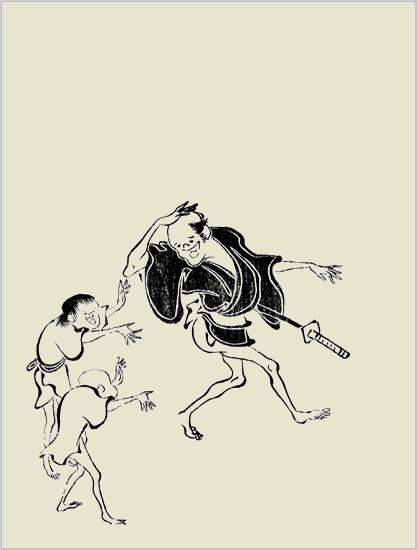
\includegraphics[width=\textwidth]{anthology-13}
\end{figure}

\begin{haiku}
    {\FH おさな子や花を見せても口を明く}\hfill{\FH 星布女}

    \vin{} The tiny child ---
    \vin{} \vin{} shown even a flower
    \vin{} \vin{} \vin{} opens its mouth \hspace{\fill} SEIFU-JO
\end{haiku}

\begin{haiku}
    {\FH 蚤の跡かぞへながらに添乳哉}\hfill{\FH 一茶}

    \vin{} Flea bites ---
    \vin{} \vin{} while counting them, she nurses
    \vin{} \vin{} \vin{} her baby \hspace{\fill} ISSA
\end{haiku}

\begin{haiku}
    {\FH \ruby{乳呑}{ちのみ}子の風よけに立かがし哉}\hfill{\FH 一茶}

    \vin{} Shielding an infant
    \vin{} \vin{} from the wind ---
    \vin{} \vin{} \vin{} a scarecrow \hspace{\fill} ISSA
\end{haiku}

\begin{haiku}
    {\FH 蝶とぶや児這ひつけばつけば又}\hfill{\FH 一茶}

    \vin{} Garden butterfly ---
    \vin{} \vin{} as the baby crawls, it flies
    \vin{} \vin{} \vin{} crawls --- flies --- \hspace{\fill} ISSA
\end{haiku}

\begin{haiku}
    {\FH 負ふた子に\ruby{蕨}{わらび}をりては持せける}\hfill{\FH 暁台}

    \vin{} A child on my back
    \vin{} \vin{} I picked a bracken shoot
    \vin{} \vin{} \vin{} and let him hold it \hspace{\fill} KY\={O}TAI
\end{haiku}

\begin{haiku}
    {\FH 渋い所母が喰けり山の柿}\hfill{\FH 一茶}

    \vin{} Her mother eats
    \vin{} \vin{} the bitter parts ---
    \vin{} \vin{} \vin{} mountain persimmons \hspace{\fill} ISSA
\end{haiku}

\begin{haiku}
    {\FH 名月を取ってくれろと泣く子哉}\hfill{\FH 一茶}

    \vin{} The harvest moon ---
    \vin{} \vin{} ``Get it for me!''
    \vin{} \vin{} \vin{} cries the child \hspace{\fill} ISSA
\end{haiku}

\begin{haiku}
    {\FH 是程のぼたんと仕かたする子哉}\hfill{\FH 一茶}

    \vin{} ``It's this big!''
    \vin{} \vin{} forming a peony with her arms ---
    \vin{} \vin{} \vin{} a child \hspace{\fill} ISSA
\end{haiku}

\begin{haiku}
    {\FH けふもけふも凧引かかる榎哉}\hfill{\FH 一茶}

    \vin{} Today too!
    \vin{} \vin{} today too! kites caught
    \vin{} \vin{} \vin{} by the nettle tree \hspace{\fill} ISSA
\end{haiku}

\begin{haiku}
    {\FH 春雨や猫におどりをおしえる子}\hfill{\FH 一茶}

    \vin{} Spring rains ---
    \vin{} \vin{} a child teaches the cat
    \vin{} \vin{} \vin{} a dance \hspace{\fill} ISSA
\end{haiku}

\begin{haiku}
    {---}\hfill{\FH 無名氏}

    \vin{} Worse than tears ---
    \vin{} \vin{} the smile of the
    \vin{} \vin{} \vin{} abandoned child \hspace{\fill} ANONYMOUS
\end{haiku}

\begin{haiku}
    {\FH 初瓜を引とらまへて寝た子哉}\hfill{\FH 一茶}

    \vin{} The season's first melon
    \vin{} \vin{} clutched in its arms
    \vin{} \vin{} \vin{} sleeps the child \hspace{\fill} ISSA
\end{haiku}

\begin{haiku}
    ---\hfill{---}

    \vin{} Blazing sun ---
    \vin{} \vin{} whose barefoot child
    \vin{} \vin{} \vin{} is running free? \hspace{\fill} K\={O}Y\={O}
\end{haiku}

\begin{haiku}
    ---\hfill{---}

    \vin{} At the ticket window
    \vin{} \vin{} our child becomes
    \vin{} \vin{} \vin{} one year younger \hspace{\fill} SEIUN
\end{haiku}

\begin{haiku}
    {---}\hfill{\FH 蕪村}

    \vin{} The youngest child
    \vin{} \vin{} visiting family graves
    \vin{} \vin{} \vin{} carries the broom \hspace{\fill} BUSON
\end{haiku}

\begin{haiku}
    {\FH 初恋や燈籠によする顔と顔}\hfill{\FH 太祇}

    \vin{} First love ---
    \vin{} \vin{} coming close to a lantern
    \vin{} \vin{} \vin{} face-to-face \hspace{\fill} TAIGI
\end{haiku}

\begin{haiku}
    {---}\hfill{\FH 無名氏}

    \vin{} Secret night rendezvous ---
    \vin{} \vin{} a mosquito was swatted
    \vin{} \vin{} \vin{} and died quietly \hspace{\fill} ANONYMOUS
\end{haiku}

\begin{haiku}
    {---}\hfill{\FH 而笑子}

    \vin{} Heaven knows,
    \vin{} \vin{} earth knows, every neighbor knows ---
    \vin{} \vin{} \vin{} parents don't know \hspace{\fill} JISH\={O}SHI
\end{haiku}

\begin{haiku}
    ---\hfill{---}

    \vin{} Sharing one umbrella ---
    \vin{} \vin{} the person more in love
    \vin{} \vin{} \vin{} gets wet \hspace{\fill} KEISANJIN
\end{haiku}

\begin{haiku}
    {---}\hfill{\FH 無名氏}

    \vin{} Catching up
    \vin{} \vin{} and looking at her ---
    \vin{} \vin{} \vin{} nothing special \hspace{\fill} ANONYMOUS
\end{haiku}

\begin{haiku}
    {---}\hfill{\FH 無名氏}

    \vin{} Hearing footsteps
    \vin{} \vin{} splitting in two
    \vin{} \vin{} \vin{} the shadow \hspace{\fill} ANONYMOUS
\end{haiku}

\begin{haiku}
    {\FH 笠でするさらばさらばや薄がすみ}\hfill{\FH 一茶}

    \vin{} Waving umbrellas
    \vin{} \vin{} ``goodbye''\ldots``goodbye''\ldots
    \vin{} \vin{} \vin{} gossamer haze \hspace{\fill} ISSA
\end{haiku}

\begin{haiku}
    {---}\hfill{\FH 無名氏}

    \vin{} Having children,
    \vin{} \vin{} you understand ---
    \vin{} \vin{} \vin{} but too late \hspace{\fill} ANONYMOUS
\end{haiku}

\begin{figure}
    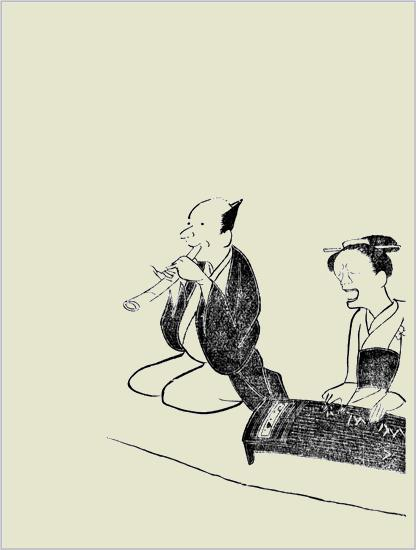
\includegraphics[width=\textwidth]{anthology-14}
\end{figure}

\begin{haiku}
    {\FH 梨の花月に\ruby{書}{ふ}ミよむ女あり}\hfill{\FH 蕪村}

    \vin{} Pear blossoms ---
    \vin{} \vin{} a woman reads a letter
    \vin{} \vin{} \vin{} by moonlight \hspace{\fill} BUSON
\end{haiku}

\begin{haiku}
    {\FH 大根引大根で道を教へけり}\hfill{\FH 一茶}

    \vin{} Harvesting radishes,
    \vin{} \vin{} he points the way
    \vin{} \vin{} \vin{} with a radish \hspace{\fill} ISSA
\end{haiku}

\begin{haiku}
    ---\hfill{---}

    \vin{} Workers ---
    \vin{} \vin{} they laugh
    \vin{} \vin{} \vin{} in a single color \hspace{\fill} HAKUSHI
\end{haiku}

\begin{haiku}
    {---}\hfill{\FH 無名氏}

    \vin{} Selling ladles,
    \vin{} \vin{} he shows how to scoop up
    \vin{} \vin{} \vin{} nothing at all \hspace{\fill} ANONYMOUS
\end{haiku}

\begin{haiku}
    {法華経の唇ばかり忙しき}\hfill{\FH 無名氏}

    \vin{} Chanting the Lotus Sutra ---
    \vin{} \vin{} only his lips
    \vin{} \vin{} \vin{} are busy \hspace{\fill} ANONYMOUS
\end{haiku}

\begin{haiku}
    {---}\hfill{\FH 無名氏}

    \vin{} With both hands
    \vin{} \vin{} thrust up mightily ---
    \vin{} \vin{} \vin{} my yawn \hspace{\fill} ANONYMOUS
\end{haiku}

\begin{haiku}
    ---\hfill{---}

    \vin{} Trout fishing ---
    \vin{} \vin{} more fishermen
    \vin{} \vin{} \vin{} than trout \hspace{\fill} KENJIN
\end{haiku}

\begin{haiku}
    {---}\hfill{\FH 無名氏}

    \vin{} Very secretly
    \vin{} \vin{} the medicine peddler
    \vin{} \vin{} \vin{} is sick \hspace{\fill} ANONYMOUS
\end{haiku}

\begin{haiku}
    {---}\hfill{\FH 無名氏}

    \vin{} The convalescent ---
    \vin{} \vin{} indulging in his mother's care
    \vin{} \vin{} \vin{} has become a habit \hspace{\fill} ANONYMOUS
\end{haiku}

\begin{haiku}
    {---}\hfill{\FH 無名氏}

    \vin{} Losing,
    \vin{} \vin{} he straightens in his seat
    \vin{} \vin{} \vin{} and loses again \hspace{\fill} ANONYMOUS
\end{haiku}

\begin{haiku}
    ---\hfill{---}

    \vin{} Having given my opinion
    \vin{} \vin{} I return home to
    \vin{} \vin{} \vin{} my wife's opinion \hspace{\fill} YACH\={O}
\end{haiku}

\begin{haiku}
    {---}\hfill{\FH 無名氏}

    \vin{} Priding himself
    \vin{} \vin{} on scolding
    \vin{} \vin{} \vin{} his beautiful wife \hspace{\fill} ANONYMOUS
\end{haiku}

\begin{figure}
    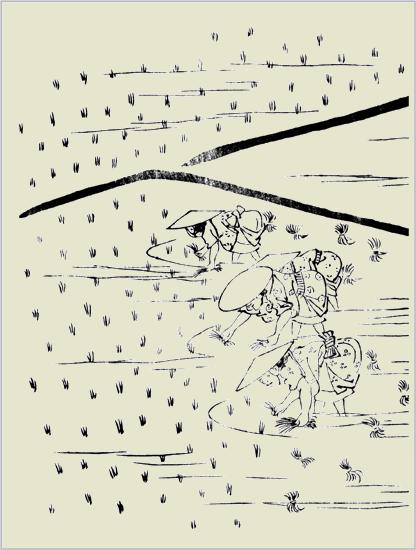
\includegraphics[width=\textwidth]{anthology-15}
\end{figure}

\begin{haiku}
    {---}\hfill{\FH 無名氏}

    \vin{} ``Every woman\ldots''
    \vin{} \vin{} he starts to say,
    \vin{} \vin{} \vin{} then looks around \hspace{\fill} ANONYMOUS
\end{haiku}

\begin{haiku}
    {---}\hfill{\FH 無名氏}

    \vin{} ``After you die
    \vin{} \vin{} they'll be valuable''
    \vin{} \vin{} \vin{} he tells the painter \hspace{\fill} ANONYMOUS
\end{haiku}

\begin{haiku}
    {\FH \ruby{骸骨}{がいこつ}の上を\ruby{装}{よそ}ふて花見かな}\hfill{\FH 鬼貫}

    \vin{} Skeletons
    \vin{} \vin{} covered with adornment ---
    \vin{} \vin{} \vin{} flower viewing \hspace{\fill} ONITSURA
\end{haiku}

\begin{haiku}
    ---\hfill{---}

    \vin{} Wanting to be logical
    \vin{} \vin{} he tries so hard ---
    \vin{} \vin{} \vin{} the drunkard \hspace{\fill} MEITEI
\end{haiku}

\begin{haiku}
    {---}\hfill{\FH 無名氏}

    \vin{} ``Let's pull them all''
    \vin{} \vin{} says the dentist
    \vin{} \vin{} \vin{} generously \hspace{\fill} ANONYMOUS
\end{haiku}

\begin{haiku}
    {\FH 負まじき角力を寝ものがたり哉}\hfill{\FH 蕪村}

    \vin{} ``I'd never lose
    \vin{} \vin{} in a sumo match'' ---
    \vin{} \vin{} \vin{} pillow talk \hspace{\fill} BUSON
\end{haiku}

\begin{haiku}
    {\FH のふなしはつみも又なし冬ごもり}\hfill{\FH 一茶}

    \vin{} No talents
    \vin{} \vin{} also no sins ---
    \vin{} \vin{} \vin{} winter seclusion \hspace{\fill} ISSA
\end{haiku}

\begin{haiku}
    {\FH 冬ごもり妻にも子にもかくれん坊}\hfill{\FH 蕪村}

    \vin{} Winter seclusion ---
    \vin{} \vin{} from my wife and children
    \vin{} \vin{} \vin{} I too play hide-and-seek \hspace{\fill} BUSON
\end{haiku}

\begin{haiku}
    ---\hfill{---}

    \vin{} New Year's cards
    \vin{} \vin{} with women's handwriting
    \vin{} \vin{} \vin{} get looked at first \hspace{\fill} BIRIKEN
\end{haiku}

\begin{haiku}
    {口聞かぬ膝へ口きく膝を乗せ}\hfill{\FH 無名氏}

    \vin{} She lowers
    \vin{} \vin{} her eloquent lap
    \vin{} \vin{} \vin{} onto his silent lap \hspace{\fill} ANONYMOUS
\end{haiku}

\begin{haiku}
    {\FH \ruby{花衣}{はなごろも}ぬぐやまつはる紐{ひも}いろいろ}\hfill{\FH 久女}

    \vin{} The kimono for flower-viewing ---
    \vin{} \vin{} disrobing, I'm entwined in
    \vin{} \vin{} \vin{} a myriad of sashes \hspace{\fill} HISA-JO
\end{haiku}

\begin{haiku}
    {\FH 物言わず客と亭主と白菊と}\hfill{\FH 蓼太}

    \vin{} Without a word
    \vin{} \vin{} the guest, the host,
    \vin{} \vin{} \vin{} white chrysanthemums \hspace{\fill} RY\={O}TA
\end{haiku}

\begin{haiku}
    {\FH 門を\ruby{出}{いず}ればわれも行人秋のくれ}\hfill{\FH 蕪村}

    \vin{} Out from the gate,
    \vin{} \vin{} I too become a traveler ---
    \vin{} \vin{} \vin{} autumn dusk \hspace{\fill} BUSON
\end{haiku}

\begin{haiku}
    {\FH 川に沿ふて行けど橋なし日の永き}\hfill{\FH 子規}

    \vin{} Walking along the river
    \vin{} \vin{} with no bridge to cross ---
    \vin{} \vin{} \vin{} the day is long \hspace{\fill} SHIKI
\end{haiku}

\begin{haiku}
    {\FH 寒月や小石のさはる\ruby{沓}{くつ}の底}\hfill{\FH 蕪村}

    \vin{} Cold moon ---
    \vin{} \vin{} feeling the pebbles
    \vin{} \vin{} \vin{} under my shoes \hspace{\fill} BUSON
\end{haiku}

\begin{haiku}
    {\FH 一人来て一人を\ruby{訪}{と}ふや秋のくれ}\hfill{\FH 蕪村}

    \vin{} A single guest
    \vin{} \vin{} visits a single host ---
    \vin{} \vin{} \vin{} autumn evening \hspace{\fill} BUSON
\end{haiku}

\begin{haiku}
    {\FH 応々と言へど\ruby{叩}{たた}くや雪の門}\hfill{\FH 去来}

    \vin{} ``Coming, coming'',
    \vin{} \vin{} but someone still knocks ---
    \vin{} \vin{} \vin{} snowy gate \hspace{\fill} KYORAI
\end{haiku}

\begin{figure}
    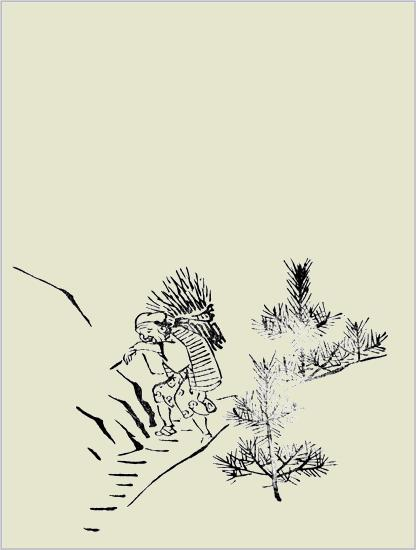
\includegraphics[width=\textwidth]{anthology-16}
\end{figure}

\begin{haiku}
    {---}\hfill{\FH 無名氏}

    \vin{} My go rival ---
    \vin{} \vin{} how vexing
    \vin{} \vin{} \vin{} and how dear \hspace{\fill} ANONYMOUS
\end{haiku}

\begin{haiku}
    {---}\hfill{\FH 宗長}

    \vin{} Getting old ---
    \vin{} \vin{} I slip on a watermelon rind
    \vin{} \vin{} \vin{} as I dance \hspace{\fill} S\={O}CH\={O}
\end{haiku}

\begin{haiku}
    {\FH はなたれて独り碁をうつ夜寒かな}\hfill{\FH 蕪村}

    \vin{} My nose running
    \vin{} \vin{} I play a solitary go-game ---
    \vin{} \vin{} \vin{} night chill \hspace{\fill} BUSON
\end{haiku}

\begin{haiku}
    ---\hfill{---}

    \vin{} Just asking them to fight,
    \vin{} \vin{} he saved tons of money
    \vin{} \vin{} \vin{} and died \hspace{\fill} HAKUCH\={O}
\end{haiku}

\begin{haiku}
    {\FH 肉がやせてくる太い骨である}\hfill{\FH 放哉}

    \vin{} Flesh getting thin ---
    \vin{} \vin{} these are thick bones \hspace{\fill} H\={O}SAI
\end{haiku}

\begin{haiku}
    {\FH 我骨のふとんにさはる霜夜哉}\hfill{\FH 蕪村}

    \vin{} Feeling my bones
    \vin{} \vin{} on the quilting ---
    \vin{} \vin{} \vin{} frosty night \hspace{\fill} BUSON
\end{haiku}

\begin{haiku}
    {\FH \ruby{炭}{すみ}の火や\ruby{齢}{よわい}のへるもあの通り}\hfill{\FH 一茶}

    \vin{} Charcoal fire ---
    \vin{} \vin{} my years dwindle down
    \vin{} \vin{} \vin{} just like that \hspace{\fill} ISSA
\end{haiku}

\begin{haiku}
    {\FH 行く我にとどまる汝に秋二つ}\hfill{\FH 子規}

    \vin{} For me leaving
    \vin{} \vin{} for you staying
    \vin{} \vin{} \vin{} two autumns \hspace{\fill} SHIKI
\end{haiku}

\begin{haiku}
    {\FH 何もないが心安さよ涼しさよ}\hfill{\FH 一茶}

    \vin{} Owning nothing ---
    \vin{} \vin{} such peace,
    \vin{} \vin{} \vin{} such coolness! \hspace{\fill} ISSA
\end{haiku}

\begin{haiku}
    {\FH 生残り生残りたる寒かな}\hfill{\FH 一茶}

    \vin{} Left to live on
    \vin{} \vin{} left to live on and on ---
    \vin{} \vin{} \vin{} this cold \hspace{\fill} ISSA
\end{haiku}

\begin{haiku}
    {\FH さびしさのうれしくもあり秋の暮}\hfill{\FH 蕪村}

    \vin{} Loneliness
    \vin{} \vin{} also has its pleasure ---
    \vin{} \vin{} \vin{} autumn dusk \hspace{\fill} BUSON
\end{haiku}

\begin{haiku}
    {\FH 身の秋や月は無きずの月ながら}\hfill{\FH 一茶}

    \vin{} Autumn of my years ---
    \vin{} \vin{} the moon is perfect
    \vin{} \vin{} \vin{} and yet --- \hspace{\fill} ISSA
\end{haiku}

\begin{haiku}
    ---\hfill{---}

    \vin{} Walking the dog
    \vin{} \vin{} you meet
    \vin{} \vin{} \vin{} lots of dogs \hspace{\fill} S\={O}SHI
\end{haiku}

\begin{haiku}
    {\FH \ruby{居眠}{いねぶ}りて我にかくれん冬ごもり}\hfill{\FH 蕪村}

    \vin{} Taking a nap
    \vin{} \vin{} I hide within myself ---
    \vin{} \vin{} \vin{} winter seclusion \hspace{\fill} BUSON
\end{haiku}

\begin{haiku}
    {\FH がつくりと抜け\ruby{初}{そめ}る歯や秋の風}\hfill{\FH 杉風}

    \vin{} All of a sudden
    \vin{} \vin{} my first fallen tooth ---
    \vin{} \vin{} \vin{} autumn wind \hspace{\fill} SANP\={U}
\end{haiku}

\begin{haiku}
    {\FH しぐるるや死なないでいる}\hfill{\FH 山頭火}

    \vin{} Winter rain ---
    \vin{} \vin{} I'm not dead yet \hspace{\fill} SANT\={O}KA
\end{haiku}

\begin{haiku}
    {\FH 家はみな杖に\ruby{白髪}{しらが}の墓参り}\hfill{\FH 芭蕉}

    \vin{} A whole family
    \vin{} \vin{} all gray-haired with canes
    \vin{} \vin{} \vin{} visits graves \hspace{\fill} BASH\={O}
\end{haiku}

\begin{haiku}
    {\FH この秋はひざに子のない月見かな}\hfill{\FH 鬼貫}

    \vin{} This autumn
    \vin{} \vin{} no child in my lap ---
    \vin{} \vin{} \vin{} moon-viewing \hspace{\fill} ONITSURA
\end{haiku}

\begin{haiku}
    {---}\hfill{\FH 無名氏}

    \vin{} Are my youthful dreams
    \vin{} \vin{} still unfinished?
    \vin{} \vin{} \vin{} this morning's frost \hspace{\fill} ANONYMOUS
\end{haiku}

\begin{haiku}
    {\FH \ruby{目出度}{めでた}さも\ruby{中}{ちう}\ruby{位也}{くらい}おらが春}\hfill{\FH 一茶}

    \vin{} The auspiciousness
    \vin{} \vin{} is just about medium ---
    \vin{} \vin{} \vin{} my spring \hspace{\fill} ISSA
\end{haiku}

\begin{haiku}
    {---}\hfill{\FH 無名氏}

    \vin{} On New Year's Day
    \vin{} \vin{} the morning in town
    \vin{} \vin{} \vin{} comes irregularly \hspace{\fill} ANONYMOUS
\end{haiku}

\begin{haiku}
    {\FH 早立のかぶせてくれし衾哉}\hfill{\FH 一茶}

    \vin{} First winter kimono ---
    \vin{} \vin{} may you quickly grow to
    \vin{} \vin{} \vin{} a naughty age \hspace{\fill} ISSA
\end{haiku}

\begin{haiku}
    {\FH 雪とけて村一ぱいの子ども哉}\hfill{\FH 一茶}

    \vin{} Snow has melted ---
    \vin{} \vin{} the village is full
    \vin{} \vin{} \vin{} of children \hspace{\fill} ISSA
\end{haiku}

\chapter{Resonance and Reverberation}

\begin{figure}
    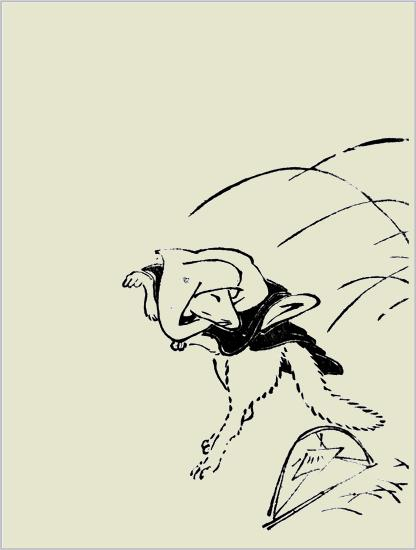
\includegraphics[width=\textwidth]{anthology-17}
\end{figure}

\begin{haiku}
    {\FH な折りそと折りてくれけり園の梅}\hfill{\FH 太祇}

    \vin{} ``Don't dare break it!''
    \vin{} \vin{} but he broke off and gave me
    \vin{} \vin{} \vin{} a branch of garden plum \hspace{\fill} TAIGI
\end{haiku}

\begin{haiku}
    {---}\hfill{\FH 破笠}

    \vin{} Spring river ---
    \vin{} \vin{} a tiny wooden clog
    \vin{} \vin{} \vin{} floats by \hspace{\fill} HARITSU
\end{haiku}

\begin{haiku}
    {\FH 春雨や薮に吹るる捨手紙}\hfill{\FH 一茶}

    \vin{} Spring rain ---
    \vin{} \vin{} blown onto the bush
    \vin{} \vin{} \vin{} a discarded letter \hspace{\fill} ISSA
\end{haiku}

\begin{haiku}
    {\FH 摘むもをしつまぬもをしき菫かな}\hfill{\FH 直女}

    \vin{} A shame to pick it
    \vin{} \vin{} a shame to leave it ---
    \vin{} \vin{} \vin{} the violet \hspace{\fill} NAO-JO
\end{haiku}

\begin{haiku}
    {\FH 追はれても急がぬふりの蝶々哉}\hfill{\FH 我樂}

    \vin{} Even when chased
    \vin{} \vin{} it pretends not to hurry ---
    \vin{} \vin{} \vin{} the butterfly \hspace{\fill} GARAKU
\end{haiku}

\begin{haiku}
    {\FH くさめして見失うたる雲雀かな}\hfill{\FH 也有}

    \vin{} One sneeze ---
    \vin{} \vin{} and I lost sight of
    \vin{} \vin{} \vin{} the skylark \hspace{\fill} YAY\={U}
\end{haiku}

\begin{haiku}
    {\FH こころ疲れて山が海が美しすぎる}\hfill{\FH 山頭火}

    \vin{} Tired heart ---
    \vin{} \vin{} mountains and ocean
    \vin{} \vin{} \vin{} too much beauty \hspace{\fill} SANT\={O}KA
\end{haiku}

\begin{haiku}
    {---}\hfill{\FH 曰人}

    \vin{} Lead him slowly!
    \vin{} \vin{} the horse is carrying
    \vin{} \vin{} \vin{} the spring moon \hspace{\fill} ATSUJIN
\end{haiku}

\begin{haiku}
    {\FH \ruby{外}{と}にも出よ触るるばかりに春の月}\hfill{\FH 汀女}

    \vin{} Come out!
    \vin{} \vin{} you can almost touch
    \vin{} \vin{} \vin{} the spring moon \hspace{\fill} TEI-JO
\end{haiku}

\begin{haiku}
    {\FH 春の月さはらば雫たりぬべし}\hfill{\FH 一茶}

    \vin{} Spring moon ---
    \vin{} \vin{} if I touch it, it would
    \vin{} \vin{} \vin{} drip \hspace{\fill} ISSA
\end{haiku}

\begin{haiku}
    {\FH 春雨や\ruby{欠}{あくび}をうつる門の犬}\hfill{\FH 一茶}

    \vin{} Spring rain ---
    \vin{} \vin{} I gave my yawn
    \vin{} \vin{} \vin{} to the dog at the gate \hspace{\fill} ISSA
\end{haiku}

\begin{haiku}
    {もの思う向こうを通るかたつむり}\hfill{\FH 無名氏}

    \vin{} While I ponder
    \vin{} \vin{} a snail
    \vin{} \vin{} \vin{} passes me by \hspace{\fill} ANONYMOUS
\end{haiku}

\begin{haiku}
    ---\hfill{---}

    \vin{} Frogs grow silent ---
    \vin{} \vin{} noble humans
    \vin{} \vin{} \vin{} are passing by \hspace{\fill} RAKUKYO
\end{haiku}

\begin{haiku}
    {---}\hfill{\FH 破笠}

    \vin{} Early summer rain ---
    \vin{} \vin{} a letter from home
    \vin{} \vin{} \vin{} arrives wet \hspace{\fill} HARITSU
\end{haiku}

\begin{haiku}
    {\FH 夕立や裸で乗しはだか馬}\hfill{\FH 一茶}

    \vin{} Sudden shower ---
    \vin{} \vin{} riding naked
    \vin{} \vin{} \vin{} on a naked horse \hspace{\fill} ISSA
\end{haiku}

\begin{haiku}
    {\FH 石も木も\ruby{眼}{まなこ}に光る暑さかな}\hfill{\FH 去来}

    \vin{} Rocks and trees
    \vin{} \vin{} glisten in my eyes ---
    \vin{} \vin{} \vin{} such heat \hspace{\fill} KYORAI
\end{haiku}

\begin{haiku}
    {\FH 石工の鑿冷したる清水かな}\hfill{\FH 蕪村}

    \vin{} The stone-carver
    \vin{} \vin{} cools his chisel
    \vin{} \vin{} \vin{} in the clear stream \hspace{\fill} BUSON
\end{haiku}

\begin{haiku}
    {\FH \ruby{鍬}{くわ}立てゝあたり人なき熱さ哉}\hfill{\FH 子規}

    \vin{} A hoe standing
    \vin{} \vin{} with no one around ---
    \vin{} \vin{} \vin{} the heat! \hspace{\fill} SHIKI
\end{haiku}

\begin{figure}
    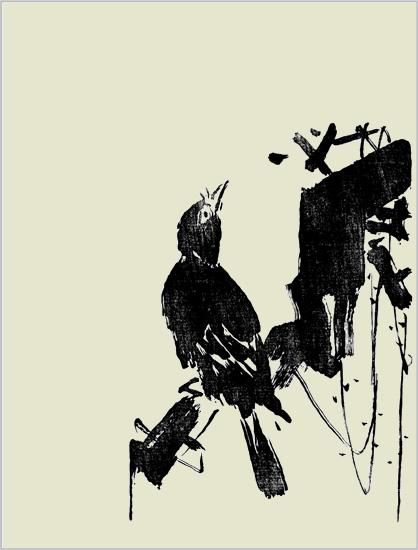
\includegraphics[width=\textwidth]{anthology-18}
\end{figure}

\begin{haiku}
    {\FH 牛に成る合点ぞ\ruby{朝寐}{あさね}夕すゞみ}\hfill{\FH 支考}

    \vin{} Becoming a cow
    \vin{} \vin{} would be fine --- morning naps
    \vin{} \vin{} \vin{} and the evening cool \hspace{\fill} SHIK\={O}
\end{haiku}

\begin{haiku}
    {---}\hfill{\FH 野水}

    \vin{} After my sneeze
    \vin{} \vin{} all is quiet ---
    \vin{} \vin{} \vin{} summer mountains \hspace{\fill} YASUI
\end{haiku}

\begin{haiku}
    {\FH 月と我ばかり残りぬ橋涼み}\hfill{\FH 菊舎}

    \vin{} Only the moon and I
    \vin{} \vin{} remain on the bridge
    \vin{} \vin{} \vin{} cooling off \hspace{\fill} KIKUSHA
\end{haiku}

\begin{haiku}
    {\FH 人一人蝿も一つや大座敷}\hfill{\FH 一茶}

    \vin{} One person
    \vin{} \vin{} and one fly
    \vin{} \vin{} \vin{} in the large room \hspace{\fill} ISSA
\end{haiku}

\begin{haiku}
    {\FH 縁の蝿手をする所を打れけり}\hfill{\FH 一茶}

    \vin{} The fly on the porch
    \vin{} \vin{} while rubbing its hands ---
    \vin{} \vin{} \vin{} swat! \hspace{\fill} ISSA
\end{haiku}

\begin{haiku}
    {\FH 蝿一つ打てはなむあみだ仏哉}\hfill{\FH 一茶}

    \vin{} Each time
    \vin{} \vin{} I swat a fly, I chant
    \vin{} \vin{} \vin{} ``Namu Amida Butsu'' \hspace{\fill} ISSA
\end{haiku}

\begin{haiku}
    {\FH ぼうふりも御経の\ruby{拍子}{ひょうし}とりにけり}\hfill{\FH 一茶}

    \vin{} Mosquito larvae,
    \vin{} \vin{} dancing a Buddhist chant
    \vin{} \vin{} \vin{} in the water by the grave \hspace{\fill} ISSA
\end{haiku}

\begin{haiku}
    {\FH 叩かれて昼の蚊を吐く木魚哉}\hfill{\FH 漱石}

    \vin{} Being hit
    \vin{} \vin{} the gong spits out
    \vin{} \vin{} \vin{} a noontime mosquito \hspace{\fill} S\={O}SEKI
\end{haiku}

\begin{haiku}
    {\FH 血を分けし身とは思はず蚊の憎き}\hfill{\FH 丈草}

    \vin{} Sharing the same blood
    \vin{} \vin{} but we're not related ---
    \vin{} \vin{} \vin{} the hateful mosquito! \hspace{\fill} J\={O}S\={O}
\end{haiku}

\begin{haiku}
    {---}\hfill{\FH 許六}

    \vin{} The flute player
    \vin{} \vin{} bitten by a mosquito
    \vin{} \vin{} \vin{} on the edge of his lips \hspace{\fill} KYOROKU
\end{haiku}

\begin{haiku}
    {\FH 蚊柱や是もなければ小淋しき}\hfill{\FH 一茶}

    \vin{} Swarms of mosquitoes ---
    \vin{} \vin{} but without them,
    \vin{} \vin{} \vin{} it's a little lonely \hspace{\fill} ISSA
\end{haiku}

\begin{haiku}
    {\FH 昼の蚊を後ろにかくす仏かな}\hfill{\FH 一茶}

    \vin{} During the day
    \vin{} \vin{} the Buddha shelters behind
    \vin{} \vin{} \vin{} mosquitoes \hspace{\fill} ISSA
\end{haiku}

\begin{figure}
    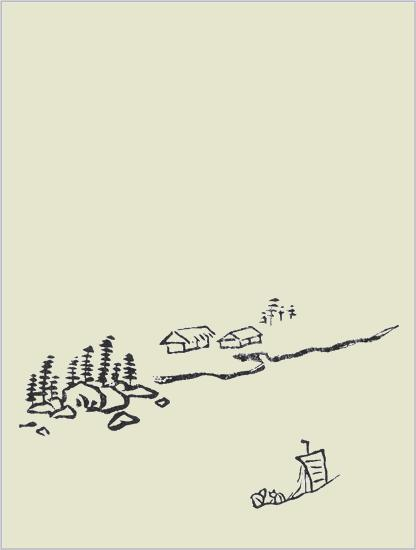
\includegraphics[width=\textwidth]{anthology-19}
\end{figure}

\begin{haiku}
    {\FH 乞食かな天地を着たる夏衣}\hfill{\FH 其角}

    \vin{} The beggar
    \vin{} \vin{} wears heaven and earth
    \vin{} \vin{} \vin{} as summer clothes \hspace{\fill} KIKAKU
\end{haiku}

\begin{haiku}
    {\FH 人有れば蝿あり仏ありにけり}\hfill{\FH 一茶}

    \vin{} Where there are people
    \vin{} \vin{} there are flies, and
    \vin{} \vin{} \vin{} there are Buddhas \hspace{\fill} ISSA
\end{haiku}

\begin{haiku}
    {\FH 長生の蝿よ蚤蚊よ貧乏村}\hfill{\FH 一茶}

    \vin{} They live long ---
    \vin{} \vin{} the flies, fleas, and mosquitoes
    \vin{} \vin{} \vin{} in this poor village \hspace{\fill} ISSA
\end{haiku}

\begin{haiku}
    {---}\hfill{\FH 無名氏}

    \vin{} Two old bent backs
    \vin{} \vin{} sitting close, wrapped in
    \vin{} \vin{} \vin{} a shower of cicada songs \hspace{\fill} ANONYMOUS
\end{haiku}

\begin{haiku}
    {\FH 手のうへにかなしく消る蛍かな}\hfill{\FH 去来}

    \vin{} In my hand
    \vin{} \vin{} its fleeting light vanishes ---
    \vin{} \vin{} \vin{} the firefly \hspace{\fill} KYORAI
\end{haiku}

\begin{haiku}
    {---}\hfill{\FH 破笠}

    \vin{} How delightful
    \vin{} \vin{} walking on dewy grasses ---
    \vin{} \vin{} \vin{} straw sandals \hspace{\fill} HARITSU
\end{haiku}

\begin{haiku}
    {\FH 蜘殺すあとの淋しき夜寒哉}\hfill{\FH 子規}

    \vin{} Killing the spider
    \vin{} \vin{} then so lonesome ---
    \vin{} \vin{} \vin{} evening cold \hspace{\fill} SHIKI
\end{haiku}

\begin{haiku}
    {\FH 年寄と見るや鳴蚊も耳の際}\hfill{\FH 一茶}

    \vin{} Seeing that I'm old
    \vin{} \vin{} even the mosquito whispers
    \vin{} \vin{} \vin{} closer to my ear \hspace{\fill} ISSA
\end{haiku}

\begin{haiku}
    {\FH 秋の蚊や死ぬる覺期でわれを刺す}\hfill{\FH 子規}

    \vin{} An autumn mosquito
    \vin{} \vin{} determined to die
    \vin{} \vin{} \vin{} bites me \hspace{\fill} SHIKI
\end{haiku}

\begin{haiku}
    {\FH 白菊にしばしたゆたふはさみかな}\hfill{\FH 蕪村}

    \vin{} Before the white chrysanthemums
    \vin{} \vin{} hesitating for a while ---
    \vin{} \vin{} \vin{} the scissors \hspace{\fill} BUSON
\end{haiku}

\begin{haiku}
    {\FH 秋来ぬと合点させたる\ruby{嚔}{くしゃみ}かな}\hfill{\FH 蕪村}

    \vin{} Truly the autumn has come ---
    \vin{} \vin{} I was convinced
    \vin{} \vin{} \vin{} by my sneeze \hspace{\fill} BUSON
\end{haiku}

\begin{haiku}
    {---}\hfill{\FH 破笠}

    \vin{} Planting my buttocks
    \vin{} \vin{} on a huge taro leaf ---
    \vin{} \vin{} \vin{} moon-viewing \hspace{\fill} HARITSU
\end{haiku}

\begin{haiku}
    {\FH 何着てもうつくしうなる月見かな}\hfill{\FH 千代女}

    \vin{} Whatever they wear
    \vin{} \vin{} they become beautiful
    \vin{} \vin{} \vin{} moon-viewing \hspace{\fill} CHIYO-JO
\end{haiku}

\begin{figure}
    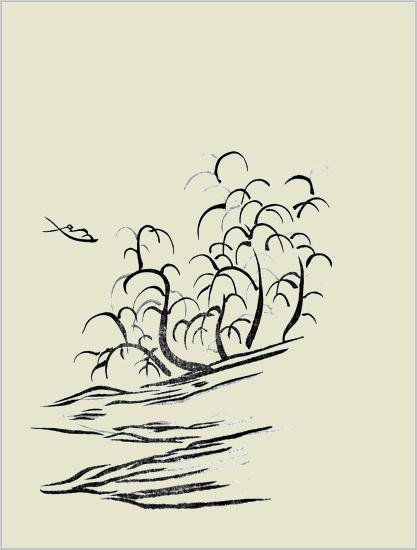
\includegraphics[width=\textwidth]{anthology-20}
\end{figure}

\begin{haiku}
    {\FH われをつれて我影帰る月見かな}\hfill{\FH 素堂}

    \vin{} Taking me along
    \vin{} \vin{} my shadow comes home
    \vin{} \vin{} \vin{} from moon-viewing \hspace{\fill} SOD\={O}
\end{haiku}

\begin{haiku}
    {\FH 婆々どのが酒呑に行く月よ哉}\hfill{\FH 一茶}

    \vin{} Even grandma
    \vin{} \vin{} goes out drinking ---
    \vin{} \vin{} \vin{} moonlit night \hspace{\fill} ISSA
\end{haiku}

\begin{haiku}
    {\FH 雁わやわやおれが噂を\ruby{致}{いた}す哉}\hfill{\FH 一茶}

    \vin{} Wild geese muttering, muttering ---
    \vin{} \vin{} are they spreading
    \vin{} \vin{} \vin{} rumors about me? \hspace{\fill} ISSA
\end{haiku}

\begin{haiku}
    {\FH 鳴な雁どつこも同じうき世ぞや}\hfill{\FH 一茶}

    \vin{} Don't cry, wild geese,
    \vin{} \vin{} it's the same everywhere ---
    \vin{} \vin{} \vin{} this floating world \hspace{\fill} ISSA
\end{haiku}

\begin{haiku}
    {---}\hfill{\FH 無名氏}

    \vin{} A man raking ---
    \vin{} \vin{} the leaves keep
    \vin{} \vin{} \vin{} calling him back \hspace{\fill} ANONYMOUS
\end{haiku}

\begin{haiku}
    {\FH 夕暮や土とかたればちる木の葉}\hfill{\FH 一茶}

    \vin{} Dusk ---
    \vin{} \vin{} while the earth and I talk
    \vin{} \vin{} \vin{} leaves fall \hspace{\fill} ISSA
\end{haiku}

\begin{haiku}
    {\FH 喜べばしきりに落つる木の実かな}\hfill{\FH 風生}

    \vin{} When I show my delight
    \vin{} \vin{} they fall down faster ---
    \vin{} \vin{} \vin{} acorns \hspace{\fill} F\={U}SEI
\end{haiku}

\begin{haiku}
    {\FH \ruby{冷冷}{ひえびえ}と袖に入る日や秋の山}\hfill{\FH 一茶}

    \vin{} Coldly, coldly
    \vin{} \vin{} the sun slips into my sleeve ---
    \vin{} \vin{} \vin{} autumn mountains \hspace{\fill} ISSA
\end{haiku}

\begin{haiku}
    {\FH 秋風や心の中の幾山河}\hfill{\FH 虚子}

    \vin{} Autumn wind ---
    \vin{} \vin{} in my heart, how many
    \vin{} \vin{} \vin{} mountains and rivers \hspace{\fill} KYOSHI
\end{haiku}

\begin{haiku}
    {\FH 山深し心に落つる秋の水}\hfill{\FH 心敬}

    \vin{} Deep in the mountains ---
    \vin{} \vin{} falling into my heart
    \vin{} \vin{} \vin{} autumn streams \hspace{\fill} SHINKEI
\end{haiku}

\begin{haiku}
    {\FH 去年より又さびいしひぞ秋の暮}\hfill{\FH 蕪村}

    \vin{} More than last year
    \vin{} \vin{} it is lonely ---
    \vin{} \vin{} \vin{} the autumn dusk \hspace{\fill} BUSON
\end{haiku}

\begin{haiku}
    {\FH 肩に来て人なつかしき赤とんぼ}\hfill{\FH 漱石}

    \vin{} On my shoulder
    \vin{} \vin{} is it longing for a companion?
    \vin{} \vin{} \vin{} a red dragonfly \hspace{\fill} S\={O}SEKI
\end{haiku}

\begin{haiku}
    {\FH 老が恋わすれんとすればしぐれかな}\hfill{\FH 蕪村}

    \vin{} Love in my old age ---
    \vin{} \vin{} as I try to forget,
    \vin{} \vin{} \vin{} late autumn rain \hspace{\fill} BUSON
\end{haiku}

\begin{haiku}
    {\FH 死んでしまへば雑草雨ふる}\hfill{\FH 山頭火}

    \vin{} When I finally die ---
    \vin{} \vin{} weeds
    \vin{} \vin{} \vin{} falling rain \hspace{\fill} SANT\={O}KA
\end{haiku}

\begin{haiku}
    {\FH 野仏の御鼻の先の氷柱哉}\hfill{\FH 一茶}

    \vin{} From the nose
    \vin{} \vin{} of the Buddha in the fields ---
    \vin{} \vin{} \vin{} icicles \hspace{\fill} ISSA
\end{haiku}

\begin{haiku}
    {\FH 来る人が道つくるなり門の雪}\hfill{\FH 一茶}

    \vin{} Visitors
    \vin{} \vin{} kindly create a path
    \vin{} \vin{} \vin{} through the snow at my gate \hspace{\fill} ISSA
\end{haiku}

\begin{haiku}
    {---}\hfill{\FH 無名氏}

    \vin{} The black dog
    \vin{} \vin{} becomes a lantern ---
    \vin{} \vin{} \vin{} snowy road \hspace{\fill} ANONYMOUS
\end{haiku}

\begin{haiku}
    {\FH 冬の日や馬上に凍る影法師}\hfill{\FH 芭蕉}

    \vin{} Winter sun ---
    \vin{} \vin{} frozen on horseback
    \vin{} \vin{} \vin{} is my shadow \hspace{\fill} BASH\={O}
\end{haiku}

\begin{haiku}
    {\FH つめたさに箒捨けり松の下}\hfill{\FH 太祇}

    \vin{} Piercing cold ---
    \vin{} \vin{} I dropped my broom
    \vin{} \vin{} \vin{} under the pines \hspace{\fill} TAIGI
\end{haiku}

\begin{haiku}
    {\FH 雪よりも寒し白髪に冬の月}\hfill{\FH 丈草}

    \vin{} Colder than snow
    \vin{} \vin{} on my white hair ---
    \vin{} \vin{} \vin{} the winter moon \hspace{\fill} J\={O}S\={O}
\end{haiku}

\begin{haiku}
    {\FH 霜百里舟中に我月を領す}\hfill{\FH 蕪村}

    \vin{} A hundred miles of frost ---
    \vin{} \vin{} in a boat, I own
    \vin{} \vin{} \vin{} the moon \hspace{\fill} BUSON
\end{haiku}

\begin{haiku}
    {\FH 安か安か寒か寒か雪雪}\hfill{\FH 山頭火}

    \vin{} Peaceful, peaceful
    \vin{} \vin{} chilly, chilly
    \vin{} \vin{} \vin{} snow, snow \hspace{\fill} SANT\={O}KA
\end{haiku}

\begin{haiku}
    {\FH ねこに来る賀状や猫のくすしより}\hfill{\FH より江}

    \vin{} To my cat
    \vin{} \vin{} a New Year's card
    \vin{} \vin{} \vin{} from its vet \hspace{\fill} YORIE
\end{haiku}

\begin{haiku}
    {\FH 膝の児の\ruby{指}{ゆびさし}始梅の花}\hfill{\FH 一茶}

    \vin{} The child on my lap
    \vin{} \vin{} begins to point at
    \vin{} \vin{} \vin{} plum blossoms \hspace{\fill} ISSA
\end{haiku}

\begin{haiku}
    {\FH 梅の花ここを盗めとさす月よ}\hfill{\FH 一茶}

    \vin{} Plum blossoms ---
    \vin{} \vin{} ``Steal this one here!''
    \vin{} \vin{} \vin{} points the moon \hspace{\fill} ISSA
\end{haiku}

\begin{haiku}
    {\FH 木のもとに汁も膾も桜かな}\hfill{\FH 芭蕉}

    \vin{} Under the trees
    \vin{} \vin{} into the salad, into the soup ---
    \vin{} \vin{} \vin{} cherry blossoms \hspace{\fill} BASH\={O}
\end{haiku}

%!TEX root = haiku.tex
\book{\LARGE \FK 杂选}

\newpage

\chapter{\FK 一}
\setcounter{haikucounter}{0}

\begin{haiku}
    {\FH 春の風草深くても\ruby[g]{古郷}{こきょう}\ruby[g]{也}{なり}}\hfill{\FH 一茶}

    {\FK 春风呵,虽然草长得深,还是故乡呵。}
\end{haiku}

\begin{haiku}
    {\FH 世の中は地獄の上の花見哉}\hfill{\FH 一茶}

    {\FK 我们在世上,边看繁花,边朝地狱行去。}
\end{haiku}

\begin{haiku}
    {\FH ままっ子や涼み仕事にわらたたき}\hfill{\FH 一茶}

    {\FK 继子呵,乘凉时候的执事是敲稻草。}
\end{haiku}

\begin{haiku}
    {\FH 正月やえたの玄関も梅の花}\hfill{\FH 一茶}

    {\FK 秽多玄关外,正月梅花开。}
\end{haiku}

\begin{haiku}
    {\FH 門の木も\ruby[g]{先}{まづ}つつがなし\ruby[g]{夕涼}{ゆうすずみ}}\hfill{\FH 一茶}

    {\FK 门前树依然无恙,好纳晚凉。}
\end{haiku}

\begin{haiku}
    {\FH わが春やたどん一つにい\ruby[g]{小菜}{こな}\ruby[g]{一把}{いちわ}}\hfill{\FH 一茶}

    {\FK 一把小菜一块煤,此乃我春天。}
\end{haiku}

\begin{haiku}
    {\FH \ruby[g]{一抱}{ひとかか}えあれど柳は柳かな}\hfill{\FH 千代女}

    {\FK 虽有一抱之粗,但柳树仍是柳树。}
\end{haiku}

\begin{haiku}
    {\FH 音\ruby[g]{添}{そ}ふて雨にしづまる\ruby[g]{碪}{きぬた}かな}\hfill{\FH 千代女}

    {\FK 秋夜里的捶衣板声,消失在雨声中。}
\end{haiku}

\begin{haiku}
    {\FH \ruby[g]{百生}{ひゃくなり}や\ruby[g]{蔓}{つる}\ruby[g]{一筋}{ひとすじ}の心より}\hfill{\FH 千代女}

    {\FK 百瓜一藤,百念皆由心生。}
\end{haiku}

\begin{haiku}
    {\FH 筆取て千艸の花におくるゝな}\hfill{\FH 闌更}

    {\FK 援笔默逊百花艳。}
\end{haiku}

\begin{haiku}
    {\FH \ruby[g]{枯蘆}{かれあし}の日に日に折れて流れけり}\hfill{\FH 闌更}

    {\FK 枯芦苇,日日折断随流去。}
\end{haiku}

\begin{haiku}
    {\FH 翡翠の影こんこんと\ruby[g]{遡}{さかのぼ}り}\hfill{\FH 茅舎}

    {\FK 翡翠鸟影,滚滚溯流上。}
\end{haiku}

\begin{haiku}
    {\FH 父が待ちし我が待ちし朴咲きにけり}\hfill{\FH 茅舎}

    {\FK 父亲等待我等待,朴树花盛开。}
\end{haiku}

\begin{haiku}
    {\FH \ruby[g]{朴散華}{ほおさんげ}\ruby[g]{即}{すなわ}ちしれぬ\ruby[g]{行方}{ゆくへ}かな}\hfill{\FH 茅舎}

    {\FK 朴树散花,不知去向。}
\end{haiku}

\begin{haiku}
    {\FH さびしさや\ruby[g]{一尺}{いちしゃく}消えてゆく蛍}\hfill{\FH 北枝}

    {\FK 流萤断续光,一明一灭一尺间,寂寞何以堪。}
\end{haiku}

\begin{haiku}
    {\FH ちぎりきな\ruby[g]{互}{かた}みに\ruby[g]{渋}{しぶ}き柿二つ}\hfill{\FH 大江丸}

    {\FK 两个涩柿子,互相摘一个。}
\end{haiku}

\begin{haiku}
    {\FH 枯野哉つばなの時の女櫛}\hfill{\FH 西鶴}

    {\FK 荒野草木枯,何人来撷茅草花,遗落小木梳。}
\end{haiku}

\begin{haiku}
    {\FH もりもり盛りあがる雲へあゆむ}\hfill{\FH 山頭火}

    {\FK 风起云涌,云涌云涌,步上白云。}
\end{haiku}

\begin{haiku}
    {\FH ひとり山越えてまた山}\hfill{\FH 山頭火}

    {\FK 不断地翻越,不断地翻越,依旧是青山。}
\end{haiku}

\begin{haiku}
    {\FH しみじみ食べる飯ばかりの飯である}\hfill{\FH 山頭火}

    {\FK 细细品味只有饭的饭。}
\end{haiku}

\begin{haiku}
    {\FH けふも\ruby[g]{托鉢}{たくはつ}こゝもかしこも花ざかり}\hfill{\FH 山頭火}

    {\FK 日日托钵,处处百花盛开。}
\end{haiku}

\begin{haiku}
    {\FH 親馬仔馬みんな戻ってくるあたゝかし}\hfill{\FH 山頭火}

    {\FK 大马小马,温暖齐归。}
\end{haiku}

\begin{haiku}
    {\FH 行く\ruby[g]{我}{われ}もにほへ花野を来る一人}\hfill{\FH 言水}

    {\FK 一人打自花野来,我亦染香花野去。}
\end{haiku}

\begin{haiku}
    {\FH 桜散る日さへ夕と成にけり}\hfill{\FH 樗良}

    {\FK 樱花飘散,朝开夕落。}
\end{haiku}

\begin{haiku}
    {\FH 子に\ruby[g]{飽}{あ}くと申す人には花もなし}\hfill{\FH 芭蕉}

    {\FK 有人不爱子,花不为伊开。}
\end{haiku}

\begin{haiku}
    {\FH 目には青葉山ほととぎす\ruby[g]{初鰹}{はつがつお}}\hfill{\FH 素堂}

    {\FK 青山绿叶杜鹃啼,更有鲣鱼初上市。}
\end{haiku}

\begin{haiku}
    {\FH かげろふやほろほろ落つる岸の砂}\hfill{\FH 土芳}

    {\FK 阳炎袅袅升,干沙簌簌落。}
\end{haiku}

\begin{haiku}
    {\FH 大原や蝶の出て舞う朧月}\hfill{\FH 丈草}

    {\FK 大原月朦胧,孤蝶翩来飞。}
\end{haiku}

\begin{haiku}
    {\FH 草霞み水に声なき日ぐれ哉}\hfill{\FH 蕪村}

    {\FK 晚霞草迷蒙,流水自无声。}
\end{haiku}

\begin{haiku}
    {\FH 風おもく人甘くなりて春くれぬ}\hfill{\FH 暁台}

    {\FK 风重人娇春将归。}
\end{haiku}

\begin{haiku}
    {\FH 萩芒来年\ruby{逢}{あは}んさりながら}\hfill{\FH 子規}

    {\FK 胡枝子和芒草,明年也想见到啊,可是啊可是。\footnote{\FT 这是子规于漱石去英国留学前,于病榻上为他写下的句子。漱石返日后,子规已病故。​​​}}
\end{haiku}

\begin{haiku}
    {\FH 春雨のわれまぼろしに近き身ぞ}\hfill{\FH 子規}

    {\FK 春雨细蒙蒙,我身近幻影。}
\end{haiku}

\begin{haiku}
    {\FH 鶯の脛の寒さよ竹の中}\hfill{\FH 紅葉}

    {\FK 竹里黄莺足胫寒。}
\end{haiku}

\begin{haiku}
    {\FH 蝶々のもの食ふ音の静かさよ}\hfill{\FH 虚子}

    {\FK 蝴蝶啮物声悄静。}
\end{haiku}

\begin{haiku}
    {\FH 日盛りに蝶のふれ合ふ音すなり}\hfill{\FH 青青}

    {\FK 盛夏阳光里,听见蝴蝶相触声。}
\end{haiku}

\begin{haiku}
    {\FH 死火山の膚つめたくて草いちご}\hfill{\FH 蛇笏}

    {\FK 死火山,冰冷山肌缀草莓。}
\end{haiku}

\begin{haiku}
    {\FH ふりかねてこよひになりぬ月の雨}\hfill{\FH 尚白}

    {\FK 忍到今宵偏月雨。}
\end{haiku}

\begin{haiku}
    {\FH 魚くふて口なまぐさし昼の雪}\hfill{\FH 成美}

    {\FK 吃鱼嘴腥味,闲看午后雪。}
\end{haiku}

\begin{haiku}
    {\FH 月さすや谷をさまよふ蛍どち}\hfill{\FH 石鼎}

    {\FK 山谷明月光,流萤皆彷徨。}
\end{haiku}

\begin{haiku}
    {\FH 花影婆娑と踏むべくありぬ岨の月}\hfill{\FH 石鼎}

    {\FK 花影婆娑欲踏踩,悬崖樱树月色明。}
\end{haiku}

\begin{haiku}
    {\FH 木より木に通へる風の春浅き}\hfill{\FH 亜浪}

    {\FK 风穿树间春初浅。}
\end{haiku}

\begin{haiku}
    {\FH ふりむけば灯とぼす関や夕霞}\hfill{\FH 太祇}

    {\FK 过得城关后,回收初看灯火瘦,天际晚霞秀。}
\end{haiku}

\begin{haiku}
    {\FH \ruby[g]{十団子}{とおだご}も\ruby[g]{小粒}{こつぶ}になりぬ秋の風}\hfill{\FH 許六}

    {\FK 萧瑟秋风起,江米团子亦变小。}
\end{haiku}

\begin{haiku}
    {\FH 蝶老いてたましひ菊にあそぶ哉}\hfill{\FH 星布女}

    {\FK 可怜蝶已老,游魂戏晚菊。}
\end{haiku}

\chapter{\FK 二}
\setcounter{haikucounter}{0}

\begin{haiku}
    {\FH あさがほに我は飯くふおとこ哉}\hfill{\FH 芭蕉}

    \vin{} Gazing at the flowers
    \vin{} \vin{} Of the morning glory,
    \vin{} \vin{} \vin{} I eat my breakfast.
\end{haiku}

\begin{haiku}
    {\FH いざ子供走りありかん玉霰}\hfill{\FH 芭蕉}

    \vin{} Look, children,
    \vin{} \vin{} Hail-stones!
    \vin{} \vin{} \vin{} Let's rush out!
\end{haiku}

\begin{haiku}
    {\FH いざ行かん雪見にころぶ所まで}\hfill{\FH 芭蕉}

    \vin{} Now let's be off!
    \vin{} \vin{} Let's go snow-viewing till
    \vin{} \vin{} \vin{} We tumble down!
\end{haiku}

\begin{haiku}
    {\FH きみ火をたけよき物見せん雪丸げ}\hfill{\FH 芭蕉}

    \vin{} You light the fire
    \vin{} \vin{} And I'll show you something nice ---
    \vin{} \vin{} \vin{} A ball of snow!
\end{haiku}

\begin{haiku}
    {\FH さびしさを問てくれぬか桐一葉}\hfill{\FH 芭蕉}

    \vin{} A paulonia leaf has fallen:
    \vin{} \vin{} Will you not come to me
    \vin{} \vin{} \vin{} In my loneliness?
\end{haiku}

\begin{haiku}
    {\FH ほととぎす大竹藪を漏る月夜}\hfill{\FH 芭蕉}

    \vin{} A cuckoo cried!
    \vin{} \vin{} The moon filters through
    \vin{} \vin{} \vin{} The vast bamboo grove.
\end{haiku}

\begin{haiku}
    {\FH ほととぎす鳴くや五尺のあやめ草}\hfill{\FH 芭蕉}

    \vin{} The voice of the cuckoo!
    \vin{} \vin{} And the tall
    \vin{} \vin{} \vin{} Irises.
\end{haiku}

\begin{haiku}
    {\FH 五月雨にかくれぬものや瀬田の橋}\hfill{\FH 芭蕉}

    \vin{} The summer rains:
    \vin{} \vin{} All things hidden
    \vin{} \vin{} \vin{} But the long bridge of Seta.
\end{haiku}

\begin{haiku}
    {\FH 何の木の花とは知らず匂ひ哉}\hfill{\FH 芭蕉}

    \vin{} The fragrance of some
    \vin{} \vin{} Unknown blossoming tree
    \vin{} \vin{} \vin{} Filled all my soul!
\end{haiku}

\begin{haiku}
    {\FH 名月や座に美しき顔もなし}\hfill{\FH 芭蕉}

    \vin{} The harvest moon!
    \vin{} \vin{} Among us, none
    \vin{} \vin{} \vin{} Has a face of beauty.
\end{haiku}

\begin{haiku}
    {\FH 命二つの中に生たる櫻かな}\hfill{\FH 芭蕉}

    \vin{} Our two lives:
    \vin{} \vin{} Between them is the life
    \vin{} \vin{} \vin{} Of the cherry flowers.
\end{haiku}

\begin{haiku}
    {\FH 手鼻かむ音さへ梅の匂ひ哉}\hfill{\FH 芭蕉}

    \vin{} The sound of someone
    \vin{} \vin{} Blowing his nose with his hand;
    \vin{} \vin{} \vin{} The scent of the plum flowers!
\end{haiku}

\begin{haiku}
    {\FH 日頃にくき烏も雪のあしたかな}\hfill{\FH 芭蕉}

    \vin{} How beautiful
    \vin{} \vin{} The usually hateful crow,
    \vin{} \vin{} \vin{} This snowy morning!
\end{haiku}

\begin{haiku}
    {\FH 晝見れば首筋赤き螢かな}\hfill{\FH 芭蕉}

    \vin{} By day-light
    \vin{} \vin{} The firefly has
    \vin{} \vin{} \vin{} A neck of red.
\end{haiku}

\begin{haiku}
    {\FH 朝顔やこれもまた我友ならず}\hfill{\FH 芭蕉}

    \vin{} The morning glory too
    \vin{} \vin{} Can never be
    \vin{} \vin{} \vin{} My friend.
\end{haiku}

\begin{haiku}
    {\FH 松茸やしらぬ木の葉のへばりつく}\hfill{\FH 芭蕉}

    \vin{} On the mushroom
    \vin{} \vin{} Is stuck the leaf
    \vin{} \vin{} \vin{} Of some unknown tree.
\end{haiku}

\begin{haiku}
    {\FH 棧や命をからむ蔦かつら}\hfill{\FH 芭蕉}

    \vin{} Ah, hanging bridge!
    \vin{} \vin{} Ivy-ropes
    \vin{} \vin{} \vin{} Entwine existence!
\end{haiku}

\begin{haiku}
    {\FH 石山の石にたばしるあられかな}\hfill{\FH 芭蕉}

    \vin{} The hail-stones
    \vin{} \vin{} Glance off the rocks
    \vin{} \vin{} \vin{} Of the Stony Mountain.
\end{haiku}

\begin{haiku}
    {\FH 稲妻に悟らぬ人の貴さよ}\hfill{\FH 芭蕉}

    \vin{} How admirable,
    \vin{} \vin{} He who thinks not, ``Life is fleeting''
    \vin{} \vin{} \vin{} When he sees the lightning-flash!
\end{haiku}

\begin{haiku}
    {\FH 聲にみな鳴きしまふてや蝉の殻}\hfill{\FH 芭蕉}

    \vin{} The shell of a cicada:
    \vin{} \vin{} It sang itself
    \vin{} \vin{} \vin{} Utterly away.
\end{haiku}

\begin{haiku}
    {\FH 葱白く洗ひたてたるさむさ哉}\hfill{\FH 芭蕉}

    \vin{} Just washed,
    \vin{} \vin{} How chill
    \vin{} \vin{} \vin{} The white leeks!
\end{haiku}

\begin{haiku}
    {\FH 蛇くふと聞けばおそろし雉子の聲}\hfill{\FH 芭蕉}

    \vin{} They say the pheasant
    \vin{} \vin{} Eats the snake;
    \vin{} \vin{} \vin{} How fearful now, its voice!
\end{haiku}

\begin{haiku}
    {\FH 馬ほくほく我を繪に見る夏野哉}\hfill{\FH 芭蕉}

    \vin{} The cob ambles slowly
    \vin{} \vin{} Across the summer moor;
    \vin{} \vin{} \vin{} I find myself in a picture.
\end{haiku}

\begin{haiku}
    {\FH 馬をさへ眺むる雪の朝かな}\hfill{\FH 芭蕉}

    \vin{} We gaze
    \vin{} \vin{} Even at horses,
    \vin{} \vin{} \vin{} This morn of snow!
\end{haiku}

\begin{haiku}
    {\FH 魂祭りけふも焼場のけぶりかな}\hfill{\FH 芭蕉}

    \vin{} The Festival of the Dead:
    \vin{} \vin{} But from the Burning-ground arises smoke,
    \vin{} \vin{} \vin{} Even today.
\end{haiku}

\begin{haiku}
    {\FH 鶯や餅に糞する椽の先}\hfill{\FH 芭蕉}

    \vin{} Look! the dried rice cakes
    \vin{} \vin{} At the end of the verandah ---
    \vin{} \vin{} \vin{} The uguisu is pooping on them!
\end{haiku}

\begin{haiku}
    {\FH 大名を馬からおろす櫻かな}\hfill{\FH 一茶}

    \vin{} The cherry blossoms!
    \vin{} \vin{} They have made a daimy\^o
    \vin{} \vin{} \vin{} Dismount from his horse.
\end{haiku}

\begin{haiku}
    {\FH 山水に米を搗かせて晝寝かな}\hfill{\FH 一茶}

    \vin{} I take a nap,
    \vin{} \vin{} Making the mountain water
    \vin{} \vin{} \vin{} Pound the rice.
\end{haiku}

\begin{haiku}
    {\FH 年玉や懐の子も手ゝをして}\hfill{\FH 一茶}

    \vin{} New Year's Presents:
    \vin{} \vin{} The baby also
    \vin{} \vin{} \vin{} Holds out its tiny hands.
\end{haiku}

\begin{haiku}
    {\FH 我味の柘榴に這す虱かな}\hfill{\FH 一茶}

    \vin{} Poor louse! I made it creep
    \vin{} \vin{} Upon the pomegranate that tastes
    \vin{} \vin{} \vin{} Of my sweet flesh.
\end{haiku}

\begin{haiku}
    {\FH 正月の子供に成って見たきかな}\hfill{\FH 一茶}

    \vin{} Ah! to be
    \vin{} \vin{} A child ---
    \vin{} \vin{} \vin{} On New Year's Day!
\end{haiku}

\begin{haiku}
    {\FH 狭くともいざ飛習へ庵の蚤}\hfill{\FH 一茶}

    \vin{} I'm sorry my house is so small,
    \vin{} \vin{} But practise your jumping,
    \vin{} \vin{} \vin{} Please, Mr.\ Flea!
\end{haiku}

\begin{haiku}
    {\FH 花の陰あかの他人はなかりけり}\hfill{\FH 一茶}

    \vin{} Beneath the cherry blossoms
    \vin{} \vin{} There are no
    \vin{} \vin{} \vin{} Strangers.
\end{haiku}

\begin{haiku}
    {\FH 鳴く猫に赤ん目をして手まりかな}\hfill{\FH 一茶}

    \vin{} The kitten is mewing;
    \vin{} \vin{} But the little girl is playing ball,
    \vin{} \vin{} \vin{} And only makes a face at him.
\end{haiku}

\begin{haiku}
    {\FH 鶯や御前へ出ても同じ聲}\hfill{\FH 一茶}

    \vin{} The nightingale!
    \vin{} \vin{} Even before His Lordship,
    \vin{} \vin{} \vin{} That same voice!
\end{haiku}

\begin{haiku}
    {\FH かたつぶり酒の肴に這はせけり}\hfill{\FH 其角}

    \vin{} Creep forward, O snail,
    \vin{} \vin{} That we may gaze on you
    \vin{} \vin{} \vin{} As relish to our wine!
\end{haiku}

\begin{haiku}
    {\FH 夕だちや家をめぐりて啼く家鴨}\hfill{\FH 其角}

    \vin{} A sudden summer shower;
    \vin{} \vin{} The ducks run round the house,
    \vin{} \vin{} \vin{} Quacking.
\end{haiku}

\begin{haiku}
    {\FH 黄菊白菊その外の名はなくもがな}\hfill{\FH 其角}

    \vin{} White chrysanthemums,
    \vin{} \vin{} Yellow chrysanthemums, ---
    \vin{} \vin{} \vin{} Would there were no other names!
\end{haiku}

\begin{haiku}
    {\FH うさくさをうしろに捨てて夏の月}\hfill{\FH 子規}

    \vin{} Behind me
    \vin{} \vin{} I cast all my care ---
    \vin{} \vin{} \vin{} The summer moon!
\end{haiku}

\begin{haiku}
    {\FH 工夫して花にランプを吊しけり}\hfill{\FH 子規}

    \vin{} Hanging a lantern on
    \vin{} \vin{} A blossoming bough ---
    \vin{} \vin{} \vin{} What pains I took!
\end{haiku}

\begin{haiku}
    {\FH 蜘蛛の巣に胡蝶のからのあはれかな}\hfill{\FH 子規}

    \vin{} In the spider's web
    \vin{} \vin{} Hang butterflies dead ---
    \vin{} \vin{} \vin{} A grievous sight!
\end{haiku}

\begin{haiku}
    {\FH 五月雨はただ降るものと覚えけり}\hfill{\FH 鬼貫}

    \vin{} I know well
    \vin{} \vin{} That the June rains
    \vin{} \vin{} \vin{} Just fall.
\end{haiku}

\begin{haiku}
    {\FH たふるればたふるるままの庭の草}\hfill{\FH 良寛}

    \vin{} The garden grasses:
    \vin{} \vin{} They fall,
    \vin{} \vin{} \vin{} And lie as they fall.
\end{haiku}

\begin{haiku}
    {\FH 盗人に取り残されし窓の月}\hfill{\FH 良寛}

    \vin{} The thief
    \vin{} \vin{} Left it behind ---
    \vin{} \vin{} \vin{} The moon at the window.
\end{haiku}

\begin{haiku}
    {\FH 鍋磨く音にまぎるる雨蛙}\hfill{\FH 良寛}

    \vin{} The sound
    \vin{} \vin{} Of the scouring of the saucepan
    \vin{} \vin{} \vin{} Blends with the green-frog's voice.
\end{haiku}

\begin{haiku}
    {\FH 雨の降る日はあはれなり良寛坊}\hfill{\FH 良寛}

    \vin{} On rainy days,
    \vin{} \vin{} The monk Ry\^okan
    \vin{} \vin{} \vin{} Feels sorry for himself.
\end{haiku}

\begin{haiku}
    {\FH 去年まで叱った瓜を手向けけり}\hfill{\FH 大江丸}

    \vin{} The melons, which last year
    \vin{} \vin{} I scolded him for eating,
    \vin{} \vin{} \vin{} I now offer to his spirit.
\end{haiku}

\begin{haiku}
    {\FH ふぐくはぬ人にはいはじ鰒の味}\hfill{\FH 大梅}

    \vin{} To a man who has not eaten
    \vin{} \vin{} A globe-fish,
    \vin{} \vin{} \vin{} We cannot speak of its flavour.
\end{haiku}

\begin{haiku}
    {\FH 名月や草木に劣る人の影}\hfill{\FH 梅室}

    \vin{} The full moon, and under the trees
    \vin{} \vin{} Their shadows --- how beautiful
    \vin{} \vin{} \vin{} Compared to mine!
\end{haiku}

\begin{haiku}
    {\FH 宿の春何もなきこそ何もあれ}\hfill{\FH 素堂}

    \vin{} In my hut this spring
    \vin{} \vin{} There is nothing ---
    \vin{} \vin{} \vin{} There is everything.
\end{haiku}

\begin{haiku}
    {\FH 廣き野をただ一のみや雉子の聲}\hfill{\FH 野明}

    \vin{} In one shrill cry
    \vin{} \vin{} The pheasant has swallowed
    \vin{} \vin{} \vin{} The broad field.
\end{haiku}

\begin{haiku}
    {\FH 御幸にも編笠ぬがぬ案山子かな}\hfill{\FH 団水}

    \vin{} Even before His Majesty,
    \vin{} \vin{} The scarecrow does not remove
    \vin{} \vin{} \vin{} Its plaited hat.
\end{haiku}

\begin{haiku}
    {\FH 月を松に懸けたり外しても見たり}\hfill{\FH 北枝}

    \vin{} I kept hanging the moon
    \vin{} \vin{} On the pine-tree and taking it off,
    \vin{} \vin{} \vin{} Gazing at it the while.
\end{haiku}

\begin{haiku}
    {\FH 流木やたぶりたぶりと春の川}\hfill{\FH 鳴雪}

    \vin{} A piece of wood ---
    \vin{} \vin{} Bobbity, bobbity it floats down
    \vin{} \vin{} \vin{} The spring river.
\end{haiku}

\begin{haiku}
    {\FH 犬を打つ石のさてなし冬の月}\hfill{\FH 太祇}

    \vin{} Not a single stone
    \vin{} \vin{} To throw at the dog, ---
    \vin{} \vin{} \vin{} wintry moon!
\end{haiku}

\begin{haiku}
    {\FH 蝶消えて魂我に返りけり}\hfill{\FH 和風}

    \vin{} The butterfly having disappeared,
    \vin{} \vin{} My spirit
    \vin{} \vin{} \vin{} Came back to me.
\end{haiku}

\begin{haiku}
    {\FH 陰に居て月に座敷をゆづりけり}\hfill{\FH 成美}

    \vin{} I sat in the shadows,
    \vin{} \vin{} And bequeathed the chamber
    \vin{} \vin{} \vin{} To the bright full moon.
\end{haiku}

\begin{haiku}
    {\FH 猫の子に嗅れてゐるや蝸牛}\hfill{\FH 才麿}

    \vin{} By a little kitten
    \vin{} \vin{} Sniffed at,
    \vin{} \vin{} \vin{} Creeps the slug unconcerned.
\end{haiku}

\begin{haiku}
    {\FH ながながと川ひとすぢや雪の原}\hfill{\FH 凡兆}

    \vin{} One long line of river
    \vin{} \vin{} Winds across
    \vin{} \vin{} \vin{} The snowy moor.
\end{haiku}

\end{document}
